%
%   $Id$
%   This file is part of the FPC documentation.
%   Copyright (C) 1997, by Michael Van Canneyt
%
%   The FPC documentation is free text; you can redistribute it and/or
%   modify it under the terms of the GNU Library General Public License as
%   published by the Free Software Foundation; either version 2 of the
%   License, or (at your option) any later version.
%
%   The FPC Documentation is distributed in the hope that it will be useful,
%   but WITHOUT ANY WARRANTY; without even the implied warranty of
%   MERCHANTABILITY or FITNESS FOR A PARTICULAR PURPOSE.  See the GNU
%   Library General Public License for more details.
%
%   You should have received a copy of the GNU Library General Public
%   License along with the FPC documentation; see the file COPYING.LIB.  If not,
%   write to the Free Software Foundation, Inc., 59 Temple Place - Suite 330,
%   Boston, MA 02111-1307, USA. 
%
\documentclass{report}
\usepackage{a4}
\usepackage{makeidx}
\usepackage{html}
\usepackage{fpc}
\usepackage{listings}
\lstset{language=delphi}
\begin{document}
%%
%   $Id$
%   This file is part of the FPC documentation.
%   Copyright (C) 1997, by Michael Van Canneyt
%
%   The FPC documentation is free text; you can redistribute it and/or
%   modify it under the terms of the GNU Library General Public License as
%   published by the Free Software Foundation; either version 2 of the
%   License, or (at your option) any later version.
%
%   The FPC Documentation is distributed in the hope that it will be useful,
%   but WITHOUT ANY WARRANTY; without even the implied warranty of
%   MERCHANTABILITY or FITNESS FOR A PARTICULAR PURPOSE.  See the GNU
%   Library General Public License for more details.
%
%   You should have received a copy of the GNU Library General Public
%   License along with the FPC documentation; see the file COPYING.LIB.  If not,
%   write to the Free Software Foundation, Inc., 59 Temple Place - Suite 330,
%   Boston, MA 02111-1307, USA. 
%
\chapter{The CRT unit.}
This chapter describes the \var{CRT} unit for Free Pascal, both under \dos
and \linux. The unit was first written for \dos by Florian kl\"ampfl. 

The unit was ported to \linux by Mark May\footnote{Current
e-mail address \textsf{mmay@dnaco.net}}, and enhanced by Micha\"el Van Canneyt
It works on the \linux console, and in xterm and rxvt windows under
X-Windows. The functionality for both is the same, except that under \linux
the use of an early implementation (versions 0.9.1 an earlier of the
compiler) the crt unit automatically cleared the screen at program startup.

This chapter is divided in two sections. 
\begin{itemize}
\item The first section lists the pre-defined constants, types and variables. 
\item The second section describes the functions which appear in the
interface part of the CRT unit.
\end{itemize}

\section{Types, Variables, Constants}
Color definitions :
\begin{verbatim}
  Black = 0;
  Blue = 1;
  Green = 2;
  Cyan = 3;
  Red = 4;
  Magenta = 5;
  Brown = 6;
  LightGray = 7;
  DarkGray = 8;
  LightBlue = 9;
  LightGreen = 10;
  LightCyan = 11;
  LightRed = 12;
  LightMagenta = 13;
  Yellow = 14;
  White = 15;
  Blink = 128;
\end{verbatim}
Miscellaneous constants
\begin{verbatim}
  TextAttr: Byte = $07;
  TextChar: Char = ' ';
  CheckBreak: Boolean = True;
  CheckEOF: Boolean = False;
  CheckSnow: Boolean = False;
  DirectVideo: Boolean = False;
  LastMode: Word = 3;
  WindMin: Word = $0;
  WindMax: Word = $184f;
  ScreenWidth = 80;
  ScreenHeight = 25;
\end{verbatim}
Some variables for compatibility with Turbo Pascal. However, they're not
used by \fpk.
\begin{verbatim}
var
  checkbreak : boolean;
  checkeof : boolean;
  checksnow : boolean;
\end{verbatim}
The following constants define screen modes on a \dos system:
\begin{verbatim}
Const
  bw40 = 0;
  co40 = 1;
  bw80 = 2;
  co80 = 3;
  mono = 7;
\end{verbatim}
The \var{TextAttr} variable controls the attributes with which characters
are written to screen.
\begin{verbatim}
var TextAttr : byte;
\end{verbatim}
The \var{DirectVideo} variable controls the writing to the screen. If it is
\var{True}, the the cursor is set via direct port access. If \var{False},
then the BIOS is used. This is defined under \dos only.
\begin{verbatim}
var DirectVideo : Boolean;
\end{verbatim}
The \var{Lastmode} variable tells you which mode was last selected for the
screen. It is defined on \dos only.
\begin{verbatim}
var lastmode : Word;
\end{verbatim}

\section{Procedures and Functions}
\procedure{AssignCrt}{(Var F: Text)}
{
Assigns a file F to the console. Everything written to the file F goes to
the console instead. If the console contains a window, everything is written
to the window instead.
}
{None.}{\seep{Window}}

\input{crtex/ex1.tex}

\procedure{Delay}{(DTime: Word)}
{Delay waits a specified number of milliseconds. The number of specified
seconds is a approximation, and may be off a lot, if system load is high.}
{None}{\seep{Sound}, \seep{NoSound}}

\input{crtex/ex15.tex}

\procedure {TextColor}{(CL: Byte)}
{
TextColor sets the foreground color to \var{CL}. \var{CL} can be one of the
predefined color constants.
}
{None.}{ \seep{TextBackground}, \seep{HighVideo}, \seep{LowVideo},
\seep{NormVideo}}

\input{crtex/ex12.tex}

\procedure {TextBackground}{(CL: Byte)}
{
TextBackground sets the background color to \var{CL}. \var{CL} can be one of the
predefined color constants.
}
{None.}{ \seep{TextColor}, \seep{HighVideo}, \seep{LowVideo},
\seep{NormVideo}}

\input{crtex/ex13.tex}

\procedure {HighVideo}{}
{ HighVideo switches the output to highlighted text. (It sets the high
intensity bit of the video attribute)
}
{None.}{ \seep{TextColor}, \seep{TextBackground}, \seep{LowVideo},
\seep{NormVideo}}

\input{crtex/ex14.tex}

\Procedure {LowVideo}
{ LowVideo switches the output to non-highlighted text. (It clears the high
intensity bit of the video attribute)
}
{None.}{ \seep{TextColor}, \seep{TextBackground}, \seep{HighVideo},
\seep{NormVideo}}

For an example, see \seep{HighVideo}

\Procedure {NormVideo}
{ NormVideo switches the output to the defaults, read at startup. (The
defaults are read from the cursor position at startup)
}
{None.}{ \seep{TextColor}, \seep{TextBackground}, \seep{LowVideo},
\seep{HighVideo}}

For an example, see \seep{HighVideo}

\Procedure{BigCursor}{Makes the cursor a big rectangle. 

Not implemented on \linux.}
{None.}{\seep{CursorOn}, \seep{CursorOff}}

\Procedure{CursorOn}{Switches the cursor on. 

Not implemented on \linux.}
{None.}{\seep{BigCursor}, \seep{CursorOff}}

\Procedure{CursorOff}{Switches the cursor off (i.e. the cursor is no
longer visible). 

Not implemented on \linux.}
{None.}{\seep{CursorOn}, \seep{BigCursor}}

\procedure {GotoXY}{(X: Byte; Y: Byte)}
{ Positions the cursor at \var{(X,Y)}, \var{X} in horizontal, \var{Y} in
vertical direction relative to the origin of the current window. The origin
is located at \var{(1,1)}, the upper-left corner of the window.
}
{None.}{ \seef{WhereX}, \seef{WhereY}, \seep{Window} }

\input{crtex/ex6.tex}

\Function  {WhereX}{Byte}
{
WhereX returns the current X-coordinate of the cursor, relative to the
current window. The origin is \var{(1,1)}, in the upper-left corner of the
window.
}
{None.}{ \seep{GotoXY}, \seef{WhereY}, \seep{Window} }


\input{crtex/ex7.tex}

\Function  {WhereY}{Byte}
{
WhereY returns the current Y-coordinate of the cursor, relative to the
current window. The origin is \var{(1,1)}, in the upper-left corner of the
window.
}
{None.}{ \seep{GotoXY}, \seef{WhereX}, \seep{Window} }

\input{crtex/ex7.tex}

\procedure {Window}{(X1, Y1, X2, Y2: Byte)}
{ Window creates a window on the screen, to which output will be sent.
\var{(X1,Y1)} are the coordinates of the upper left corner of the window,
\var{(X2,Y2)} are the coordinates of the bottom right corner of the window.
These coordinates are relative to the entire screen, with the top left
corner equal to \var{(1,1)}

Further coordinate operations, except for the next Window call,
are relative to the window's top left corner.
}
{None.}{\seep{GotoXY}, \seef{WhereX}, \seef{WhereY}, \seep{ClrScr}}

\input{crtex/ex5.tex}


\procedure {ClrScr}{}
{ ClrScr clears the current window (using the current colors), 
and sets the cursor in the top left
corner of the current window.}
{None.}{ \seep{Window} }

\input{crtex/ex8.tex}


%\procedure {ScrollWindow}{(X1,Y1,X2,Y2 : Byte; Count : Longint)}
%{ ScrollWindow scrolls the contents of the window defined by the upper-left
%\var{(X1,Y1)} and lower-right \var{(X2,Y2)} corners \var{count} lines up if
%\var{count} is positive, it scrolls down if \var{count} is negative.
%The new lines are made blank using the current textcolors.
%}
%{None.}{\seep{Window}, \seep{ClrScr}}

%\function {SaveScreenRegion}{(X1,Y1,X2,Y2, var P : pointer)}{Boolean}
%{SaveScreenRegion writes the the contents of the window defined by the upper-left
%\var{(X1,Y1)} and lower-right \var{(X2,Y2)} corners to the location pointed
%to by \var{P}. If \var{P} is \var{nil} then enough memory is allocated to
%contain the contents of the window.
%
%The contents are written as follows : line per line, column per column,
%first the character on screen is written (1 byte), followed by the text 
%attribute (1 byte). The size required is therefore 
%\var{(Y2-Y1+1)*(X2-X1+1)*2} bytes.
%
%The function returns \var{False} if it couldn't allocate the required
%memory, \var{True} if the memory was allocated.}{None.}
%{\seep{RestoreScreenRegion}, \seep{Window} }

%\procedure {RestoreScreenRegion}{(X1,Y1,X2,Y2, var P : pointer)}
%{SaveScreenRegion writes the the contents of the memory location pointed to
%by \var{P}, to the window defined by the upper-left \var{(X1,Y1)} and 
%lower-right \var{(X2,Y2)} corners. 
%
%The contents of \var{P} should be arranged as if they are when written by 
%a call to the SaveScreenRegion () function.
%
%The memory pointed to by \var{P} is NOT freed.}{None}
%{\seef{SaveScreenRegion}, \seep{Window} }


\Procedure {ClrEol}
{ ClrEol clears the current line, starting from the cursor position, to the
end of the window. The cursor doesn't move}
{None.}{\seep{DelLine}, \seep{InsLine}, \seep{ClrScr}}

\input{crtex/ex9.tex}


\Procedure {DelLine}
{ DelLine removes the current line. Lines following the current line are 
scrolled 1 line up, and an empty line is inserted at the bottom of the
current window. The cursor doesn't move.}
{None.}{\seep{ClrEol}, \seep{InsLine}, \seep{ClrScr}}

\input{crtex/ex11.tex}


\procedure {InsLine}{}
{ InsLine inserts an empty line at the current cursor position. 
Lines following the current line are scrolled 1 line down, 
causing the last line to disappear from the window. 
The cursor doesn't move.}
{None.}{\seep{ClrEol}, \seep{DelLine}, \seep{ClrScr}}

\input{crtex/ex10.tex}


\Function {KeyPressed}{Boolean}
{ The Keypressed function scans the keyboard buffer and sees if a key has
been pressed. If this is the case, \var{True} is returned. If not,
\var{False} is returned. The \var{Shift, Alt, Ctrl} are not reported.
The key is not removed from the buffer, and can hence still be read after
the KeyPressed function has been called.
}
{None.}{\seef{ReadKey}}

\input{crtex/ex2.tex}


\Function  {ReadKey}{Char}
{
The ReadKey function reads 1 key from the keyboard buffer, and returns this.
If an extended or function key has been pressed, then the zero ASCII code is 
returned. You can then read the scan code of the key with a second ReadKey
call.

\textbf{Remark.} Key mappings under Linux can cause the wrong key to be
reported by ReadKey, so caution is needed when using ReadKey.  
}
{None.}{\seef{KeyPressed}}

\input{crtex/ex3.tex}


\procedure{Sound}{(hz : word)}
{ Sounds the speaker at a frequency of \var{hz}.

This is not supported in \linux}{None.}{\seep{NoSound}}
\Procedure{NoSound}{
Stops the speaker sound.

This is not supported in \linux}{None.}{\seep{Sound}}

\input{crtex/ex16.tex}


%%
%   $Id$
%   This file is part of the FPC documentation.
%   Copyright (C) 1997, by Michael Van Canneyt
%
%   The FPC documentation is free text; you can redistribute it and/or
%   modify it under the terms of the GNU Library General Public License as
%   published by the Free Software Foundation; either version 2 of the
%   License, or (at your option) any later version.
%
%   The FPC Documentation is distributed in the hope that it will be useful,
%   but WITHOUT ANY WARRANTY; without even the implied warranty of
%   MERCHANTABILITY or FITNESS FOR A PARTICULAR PURPOSE.  See the GNU
%   Library General Public License for more details.
%
%   You should have received a copy of the GNU Library General Public
%   License along with the FPC documentation; see the file COPYING.LIB.  If not,
%   write to the Free Software Foundation, Inc., 59 Temple Place - Suite 330,
%   Boston, MA 02111-1307, USA. 
%
\chapter{The DOS unit.}
\FPCexampledir{dosex}

This chapter describes the \var{DOS} unit for Free pascal. The \var{DOS}
unit gives access to some operating system calls related to files, the
file system, date and time. Except for the \palmos target, this unit is
available to all supported platforms.

The unit was first written for \dos by Florian Kl\"ampfl. It was ported to 
\linux by Mark May\footnote{Current e-mail address \textsf{mmay@dnaco.net}}, 
and enhanced by Micha\"el Van Canneyt. The \amiga version was ported by
Nils Sjoholm.

Under non-\dos systems, some of the functionality is lost, as it is either impossible 
or meaningless to implement it. Other than that, the functionality for all 
operating systems is the same.

This chapter is divided in three sections:
\begin{itemize}
\item The first section lists the pre-defined constants, types and variables. 
\item The second section gives an overview of all functions available,
grouped by category.
\item The third section describes the functions which appear in the
interface part of the DOS unit.
\end{itemize}

\section{Types, Variables, Constants}


\subsection {Constants}
The DOS unit implements the following constants:

\subsubsection{File attributes}

The File Attribute constants are used in \seep{FindFirst}, \seep{FindNext} to
determine what type of special file to search for in addition to normal files. 
These flags are also used in the \seep{SetFAttr} and \seep{GetFAttr} routines to 
set and retrieve attributes of files. For their definitions consult 
\seet{fileattributes}.

\begin{FPCltable}{lll}{Possible file attributes}{fileattributes}
\hline
Constant & Description & Value\\ \hline
\var{readonly} & Read only file & \$01\\
\var{hidden} & Hidden file & \$02 \\
\var{sysfile} & System file & \$04\\
\var{volumeid} & Volume label & \$08\\
\var{directory} & Directory & \$10\\
\var{archive} & Archive & \$20\\ 
\var{anyfile} & Any of the above special files & \$3F\\
\hline
\end{FPCltable}

\subsubsection{fmXXXX}

These constants are used in the \var{Mode} field of the \var{TextRec}
record. Gives information on the filemode of the text I/O. For their
definitions consult \seet{fmxxxconstants}.

\begin{FPCltable}{lll}{Possible mode constants}{fmxxxconstants}
\hline
Constant & Description & Value\\ \hline
\var{fmclosed} & File is closed & \$D7B0\\
\var{fminput} & File is read only & \$D7B1 \\
\var{fmoutput} & File is write only & \$D7B2\\
\var{fminout} & File is read and write & \$D7B3\\
\hline
\end{FPCltable}

\subsubsection{Other}

The following constants are not portable, and should not be used. They
are present for compatibility only.

\begin{verbatim}
  {Bitmasks for CPU Flags}
  fcarry =     $0001;
  fparity =    $0004;
  fauxiliary = $0010;
  fzero =      $0040;
  fsign =      $0080;
  foverflow  = $0800;
\end{verbatim}  
  
\subsection{Types}
The following string types are defined for easy handling of
filenames :
\begin{verbatim}
  ComStr  = String[255];   { For command-lines } 
  PathStr = String[255];   { For full path for file names }
  DirStr  = String[255];   { For Directory and (DOS) drive string }
  NameStr = String[255];   { For Name of file }
  ExtStr  = String[255];   { For Extension of file }
\end{verbatim}
\begin{verbatim}
  SearchRec = Packed Record
    Fill : array[1..21] of byte;  
    { Fill replaced with declarations below, for Linux}
    Attr : Byte; {attribute of found file}
    Time : LongInt; {last modify date of found file}
    Size : LongInt; {file size of found file}
    Reserved : Word; {future use}
    Name : String[255]; {name of found file}
    SearchSpec: String[255]; {search pattern}
    NamePos: Word; {end of path, start of name position}
    End;
\end{verbatim}
Under \linux, the \var{Fill} array is replaced with the following:
\begin{verbatim}
    SearchNum: LongInt; {to track which search this is}
    SearchPos: LongInt; {directory position}
    DirPtr: LongInt; {directory pointer for reading directory}
    SearchType: Byte;  {0=normal, 1=open will close}
    SearchAttr: Byte; {attribute we are searching for}
    Fill: Array[1..07] of Byte; {future use}
\end{verbatim}
This is because the searching meachanism on Unix systems is substantially
different from \dos's, and the calls have to be mimicked.
\begin{verbatim}
const
  filerecnamelength = 255;
type
  FileRec = Packed Record
    Handle,
    Mode,  
    RecSize   : longint;
    _private  : array[1..32] of byte;
    UserData  : array[1..16] of byte;
    name      : array[0..filerecnamelength] of char;
  End;
\end{verbatim}
\var{FileRec} is used for internal representation of typed and untyped files.
Text files are handled by the following types :
\begin{verbatim}
const
  TextRecNameLength = 256;
  TextRecBufSize    = 256;
type
  TextBuf = array[0..TextRecBufSize-1] of char;
  TextRec = Packed Record
    Handle,
    Mode,  
    bufsize,
    _private,
    bufpos,  
    bufend    : longint;
    bufptr    : ^textbuf;
    openfunc,
    inoutfunc,
    flushfunc,
    closefunc : pointer;
    UserData  : array[1..16] of byte;
    name      : array[0..textrecnamelength-1] of char;
    buffer    : textbuf;
  End;
\end{verbatim}
Remark that this is not binary compatible with the Turbo Pascal definition
of \var{TextRec}, since the sizes of the different fields are different.
\begin{verbatim}
    Registers = record
      case i : integer of
        0 : (ax,f1,bx,f2,cx,f3,dx,f4,bp,f5,si,
             f51,di,f6,ds,f7,es,f8,flags,fs,gs : word);
        1 : (al,ah,f9,f10,bl,bh,f11,f12,
             cl,ch,f13,f14,dl,dh : byte);
        2 : (eax,  ebx,  ecx,  edx,  ebp,  esi,  edi : longint);
        End;
\end{verbatim}
The  \var{registers} type is used in the \var{MSDos} call.
\begin{verbatim}
  DateTime = record
    Year: Word;
    Month: Word;
    Day: Word;
    Hour: Word;
    Min: Word;
    Sec: word;
    End;
\end{verbatim}
The \var{DateTime} type is used in \seep{PackTime} and \seep{UnPackTime} for
setting/reading file times with \seep{GetFTime} and \seep{SetFTime}.
\subsection{Variables}
\begin{verbatim}
    DosError : integer;
\end{verbatim}
The \var{DosError} variable is used by the procedures in the \dos unit to 
report errors. It can have the following values :
\begin{center}
\begin{tabular}{cl}
2 & File not found. \\
3 & path not found. \\
5 & Access denied. \\
6 & Invalid handle. \\
8 & Not enough memory. \\
10 & Invalid environment. \\
11 & Invalid format. \\
18 & No more files.
\end{tabular}
\end{center}
Other values are possible, but are not documented.
%\begin{verbatim}
%    drivestr : array [0..26] of pchar;
%\end{verbatim}
%This variable is defined in the \linux version of the \dos unit. It is used
%in the \seef{DiskFree} and \seef{DiskSize} calls.

%%%%%%%%%%%%%%%%%%%%%%%%%%%%%%%%%%%%%%%%%%%%%%%%%%%%%%%%%%%%%%%%%%%%%%%
% Functions and procedures by category
\section{Function list by category}
What follows is a listing of the available functions, grouped by category.
For each function there is a reference to the page where you can find the
function.

\subsection{File handling}
Routines to handle files on disk.
\begin{funclist}
\funcrefl{FExpand}{Dos:FExpand}{Expand filename to full path}
\procref{FindClose}{Close finfirst/findnext session}
\procref{FindFirst}{Start find of file}
\procref{FindNext}{Find next file}
\funcrefl{FSearch}{Dos:FSearch}{Search for file in a path}
\procref{FSplit}{Split filename in parts}
\procref{GetFAttr}{Return file attributes}
\procref{GetFTime}{Return file time}
\funcref{GetLongName}{Convert short filename to long filename (DOS only)}
\funcref{GetShortName}{Convert long filename to short filename (DOS only)}
\procref{SetFAttr}{Set file attributes}
\procref{SetFTime}{Set file time}
\end{funclist}

\subsection{Directory and disk handling}
Routines to handle disk information.
\begin{funclist}
\procref{AddDisk}{Add disk to list of disks (UNIX only)}
\funcref{DiskFree}{Return size of free disk space}
\funcref{DiskSize}{Return total disk size}
\end{funclist}

\subsection{Process handling}
Functions to handle process information and starting new processes.
\begin{funclist}
\funcref{DosExitCode}{Exit code of last executed program}
\funcref{EnvCount}{Return number of environment variables}
\funcref{EnvStr}{Return environment string pair}
\procref{Exec}{Execute program}
\funcrefl{GetEnv}{Dos:GetEnv}{Return specified environment string}
\end{funclist}

\subsection{System information}
Functions for retrieving and setting general system information such as date
and time.
\begin{funclist}
\funcref{DosVersion}{Get OS version}
\procref{GetCBreak}{Get setting of control-break handling flag}
\procrefl{GetDate}{Dos:GetDate}{Get system date}
\procref{GetIntVec}{Get interrupt vector status}
\procrefl{GetTime}{Dos:GetTime}{Get system time}
\procref{GetVerify}{Get verify flag}
\procref{Intr}{Execute an interrupt}
\procref{Keep}{Keep process in memory and exit}
\procref{MSDos}{Execute MS-dos function call}
\procref{PackTime}{Pack time for file time}
\procref{SetCBreak}{Set control-break handling flag}
\procref{SetDate}{Set system date}
\procref{SetIntVec}{Set interrupt vectors}
\procref{SetTime}{Set system time}
\procref{SetVerify}{Set verify flag}
\procref{SwapVectors}{Swap interrupt vectors}
\procref{UnPackTime}{Unpack file time}
\end{funclist}

%%%%%%%%%%%%%%%%%%%%%%%%%%%%%%%%%%%%%%%%%%%%%%%%%%%%%%%%%%%%%%%%%%%%%%%
% Functions and procedures
\section{Functions and Procedures}
\begin{procedure}{AddDisk}
\Declaration
Procedure AddDisk (Const S : String);
\Description
\var{AddDisk} adds a filename \var{S} to the internal list of disks. It is
implemented for systems which do not use DOS type drive letters.
 This list is used to determine which disks to use in the \seef{DiskFree}
and \seef{DiskSize} calls. 
The \seef{DiskFree} and \seef{DiskSize} functions need a file on the 
specified drive, since this is required for the \var{statfs} system call.
The names are added sequentially. The dos
initialization code presets the first three disks to:
\begin{itemize}
\item \var{'.'} for the current drive, 
\item \var{'/fd0/.'} for the first floppy-drive (linux only).
\item \var{'/fd1/.'} for the second floppy-drive (linux only).
\item \var{'/'} for the first hard disk.
\end{itemize}
The first call to \var{AddDisk} will therefore add a name for the second
harddisk, The second call for the third drive, and so on until 23 drives
have been added (corresponding to drives \var{'D:'} to \var{'Z:'})
\Errors
None
\SeeAlso
\seef{DiskFree}, \seef{DiskSize} 
\end{procedure}


\begin{function}{DiskFree}
\Declaration
Function DiskFree (Drive: byte) : int64;
\Description

\var{DiskFree} returns the number of free bytes on a disk. The parameter
\var{Drive} indicates which disk should be checked. This parameter is 1 for
floppy \var{a:}, 2 for floppy \var{b:}, etc. A value of 0 returns the free
space on the current drive. 

\textbf{For \unix only:}\\
The \var{diskfree} and \var{disksize} functions need a file on the 
specified drive, since this is required for the \var{statfs} system call.
These filenames are set in the initialization of the dos unit, and have 
been preset to :
\begin{itemize}
\item \var{'.'} for the current drive, 
\item \var{'/fd0/.'} for the first floppy-drive (linux only).
\item \var{'/fd1/.'} for the second floppy-drive (linux only).
\item \var{'/'} for the first hard disk.
\end{itemize}
There is room for 1-26 drives. You can add a drive with the
\seep{AddDisk} procedure.
These settings can be coded in \var{dos.pp}, in the initialization part.

\Errors
-1 when a failure occurs, or an invalid drive number is given.
\SeeAlso
\seef{DiskSize}, \seep{AddDisk}
\end{function}

\FPCexample{ex6}

\begin{function}{DiskSize}
\Declaration
Function DiskSize (Drive: byte) : int64;
\Description

\var{DiskSize} returns the total size (in bytes) of a disk. The parameter
\var{Drive} indicates which disk should be checked. This parameter is 1 for
floppy \var{a:}, 2 for floppy \var{b:}, etc. A value of 0 returns the size
of the current drive. 

\textbf{For \unix only:}\\
The \var{diskfree} and \var{disksize} functions need a file on the specified drive, since this
is required for the \var{statfs} system call.
  These filenames are set in the initialization of the dos unit, and have 
been preset to :
\begin{itemize}
\item \var{'.'} for the current drive, 
\item \var{'/fd0/.'} for the first floppy-drive (linux only).
\item \var{'/fd1/.'} for the second floppy-drive (linux only).
\item \var{'/'} for the first hard disk.
\end{itemize}
There is room for 1-26 drives. You can add a drive with the
\seep{AddDisk} procedure.
These settings can be coded in \var{dos.pp}, in the initialization part.

\Errors
-1 when a failure occurs, or an invalid drive number is given.
\SeeAlso
\seef{DiskFree}, \seep{AddDisk}
\end{function}
For an example, see \seef{DiskFree}.
\begin{function}{DosExitCode}
\Declaration
Function DosExitCode  : Word;
\Description

\var{DosExitCode} contains (in the low byte) the exit-code of a program 
executed with the \var{Exec} call.
\Errors
None.
\SeeAlso
\seep{Exec}
\end{function}

\FPCexample{ex5}

\begin{function}{DosVersion}
\Declaration
Function DosVersion  : Word;
\Description
\var{DosVersion} returns the operating system or kernel version. The
low byte contains the major version number, while the high byte 
contains the minor version number.
\Portability
On systems where versions consists of more then two numbers, 
only the first two numbers will be returned. For example Linux version 2.1.76 
will give you DosVersion 2.1. Some operating systems, such as \freebsd, do not
have system calls to return the kernel version, in that case a value of 0 will
be returned.
\Errors
None.
\SeeAlso

\end{function}


\FPCexample{ex1}


\begin{function}{EnvCount}
\Declaration
Function EnvCount  : longint;\Description
\var{EnvCount} returns the number of environment variables.
\Errors
None.
\SeeAlso
\seef{EnvStr}, \seef{Dos:GetEnv}
\end{function}

\begin{function}{EnvStr}
\Declaration
Function EnvStr (Index: integer) : string;\Description

\var{EnvStr} returns the \var{Index}-th \var{Name=Value} pair from the list
of environment variables. 
The index of the first pair is zero.
\Errors
The length is limited to 255 characters. 
\SeeAlso
\seef{EnvCount}, \seef{Dos:GetEnv}
\end{function}

\FPCexample{ex13}

\begin{procedure}{Exec}
\Declaration
Procedure Exec (const Path: pathstr; const ComLine: comstr);
\Description

\var{Exec} executes the program in \var{Path}, with the options given by
\var{ComLine}.
After the program has terminated, the procedure returns. The Exit value of
the program can be consulted with the \var{DosExitCode} function.

\Errors
Errors are reported in \var{DosError}.
\SeeAlso
\seef{DosExitCode}
\end{procedure}
For an example, see \seef{DosExitCode}
\begin{functionl}{FExpand}{Dos:FExpand}
\Declaration
Function FExpand (const path: pathstr) : pathstr;
\Description

\var{FExpand} takes its argument and expands it to a complete filename, i.e.
a filename starting from the root directory of the current drive, prepended
with the drive-letter or volume name (when supported).
\Portability
On case sensitive file systems (such as \unix and \linux), the resulting
name is left as it is, otherwise it is converted to uppercase.
\Errors
\seep{FSplit}
\SeeAlso
\end{functionl}

\FPCexample{ex5}

\begin{procedure}{FindClose}
\Declaration
Procedure FindClose (Var F: SearchRec);
\Description
\var{FindClose} frees any resources associated with the search record
\var{F}.

This call is needed to free any internal resources allocated by the 
\seef{FindFirst} or \seef{FindNext} calls.


The \linux implementation of the \dos unit therefore keeps a table of open
directories, and when the table is full, closes one of the directories, and
reopens another. This system is adequate but slow if you use a lot of
\var{searchrecs}.
So, to speed up the findfirst/findnext system, the \var{FindClose} call was
implemented. When you don't need a \var{searchrec} any more, you can tell
this to the \dos unit by issuing a \var{FindClose} call. The directory
which is kept open for this \var{searchrec} is then closed, and the table slot
freed.

\Portability
It is recommended to use the \linux call \var{Glob} when looking for files 
on \linux.

\Errors
Errors are reported in DosError.
\SeeAlso
\seef{Glob}.
\end{procedure}

\begin{procedure}{FindFirst}
\Declaration
Procedure FindFirst (const Path: pathstr; Attr: word; var F: SearchRec);
\Description

\var{FindFirst} searches the file specified in \var{Path}. Normal files,
as well as all special files which have the attributes specified in
\var{Attr} will be returned.

It returns a \var{SearchRec} record for further searching in \var{F}.
\var{Path} can contain the wildcard characters \var{?} (matches any single
character) and \var{*} (matches 0 ore more arbitrary characters). In this
case \var{FindFirst} will return the first file which matches the specified
criteria.
If \var{DosError} is different from zero, no file(s) matching the criteria 
was(were) found.

\Portability
On \ostwo, you cannot issue two different \var{FindFirst} calls. That is,
you must close any previous search operation with \seep{FindClose} before
starting a new one. Failure to do so will end in a Run-Time Error 6 
(Invalid file handle)

\Errors
Errors are reported in DosError.
\SeeAlso
\seep{FindNext},
\seep{FindClose}
\end{procedure}

\FPCexample{ex7}

\begin{procedure}{FindNext}
\Declaration
Procedure FindNext (var f: searchRec);
\Description

\var{FindNext} takes as an argument a \var{SearchRec} from a previous
\var{FindNext} call, or a \var{FindFirst} call, and tries to find another
file which matches the criteria, specified in the \var{FindFirst} call.
If \var{DosError} is different from zero, no more files matching the
criteria were found.
\Errors
\var{DosError} is used to report errors.
\SeeAlso
\seep{FindFirst}, \seep{FindClose}
\end{procedure}
For an example, see \seep{FindFirst}.
\begin{functionl}{FSearch}{Dos:FSearch}
\Declaration
Function FSearch (Path: pathstr; DirList: string) : pathstr;
\Description
\var{FSearch} searches the file \var{Path} in all directories listed in
\var{DirList}. The full name of the found file is returned.
\var{DirList} must be a list of directories, separated by semi-colons.
When no file is found, an empty string is returned.
\Portability
On \unix systems, \var{DirList} can also be separated by colons, as is
customary on those environments.
\Errors
None.
\SeeAlso
\seefl{FExpand}{Dos:FExpand}
\end{functionl}

\FPCexample{ex10}

 
\begin{procedure}{FSplit}
\Declaration
Procedure FSplit (path: pathstr; \\ var dir: dirstr; var name: namestr;
  var ext: extstr);
\Description

\var{FSplit} splits a full file name into 3 parts : A \var{Path}, a
\var{Name} and an extension  (in \var{ext}.) 
The extension is taken to be all letters after the {\em last} dot (.). For 
\dos, however, an exception is made when \var{LFNSupport=False}, then
the extension is defined as all characters after the {\em first} dot.

\Errors
None.
\SeeAlso
\seefl{FSearch}{Dos:FSearch}
\end{procedure}

\FPCexample{ex12}

\begin{procedure}{GetCBreak}
\Declaration
Procedure GetCBreak (var breakvalue: boolean);
\Description

\var{GetCBreak} gets the status of CTRL-Break checking under \dos and \amiga.
When \var{BreakValue} is \var{false}, then \dos only checks for the 
CTRL-Break key-press when I/O is performed. When it is set to \var{True},
then a check is done at every system call.
\Portability
Under non-\dos and non-\amiga operating systems, \var{BreakValue} always returns 
\var{True}.
\Errors 
None
\SeeAlso
\seep{SetCBreak}
\end{procedure}

\begin{procedurel}{GetDate}{Dos:GetDate}
\Declaration
Procedure GetDate (var year, month, mday, wday: word);\Description

\var{GetDate} returns the system's date. \var{Year} is a number in the range
1980..2099.\var{mday} is the day of the month,
\var{wday} is the day of the week, starting with Sunday as day 0.
\Errors
None.
\SeeAlso
\seepl{GetTime}{Dos:GetTime},\seep{SetDate}
\end{procedurel}

\FPCexample{ex2}

\begin{functionl}{GetEnv}{Dos:GetEnv}
\Declaration
Function GetEnv (EnvVar: String) : String;
\Description

\var{Getenv} returns the value of the environment variable \var{EnvVar}.
When there is no environment variable \var{EnvVar} defined, an empty
string is returned.
\Portability
Under some operating systems (such as \unix), case is important when looking
for \var{EnvVar}.
\Errors
None.
\SeeAlso
\seef{EnvCount}, \seef{EnvStr}
\end{functionl}

\FPCexample{ex14}

\begin{procedure}{GetFAttr}
\Declaration
Procedure GetFAttr (var F; var Attr: word);
\Description

\var{GetFAttr} returns the file attributes of the file-variable \var{f}.
 \var{F} can be a untyped or typed file, or of type \var{Text}. \var{f} must
have been assigned, but not opened. The attributes can be examined with the
following constants :
\begin{itemize}
\item \var{ReadOnly}
\item \var{Hidden}
\item \var{SysFile}
\item \var{VolumeId}
\item \var{Directory}
\item \var{Archive}
\end{itemize}
Under \linux, supported attributes are:
\begin{itemize}
\item \var{Directory}
\item \var{ReadOnly} if the current process doesn't have access to the file.
\item \var{Hidden} for files whose name starts with a dot \var{('.')}.
\end{itemize}

\Errors
Errors are reported in \var{DosError}
\SeeAlso
\seep{SetFAttr}
\end{procedure}

\FPCexample{ex8}

\begin{procedure}{GetFTime}
\Declaration
Procedure GetFTime (var F; var Time: longint);
\Description

\var{GetFTime} returns the modification time of a file.
This time is encoded and must be decoded with \var{UnPackTime}. 
\var{F} must be a file type, which has been assigned, and
opened.
\Errors
Errors are reported in \var{DosError}
\SeeAlso
\seep{SetFTime}, \seep{PackTime},\seep{UnPackTime}
\end{procedure}

\FPCexample{ex9}

\begin{procedure}{GetIntVec}
\Declaration
Procedure GetIntVec (IntNo: byte; var Vector: pointer);
\Description

\var{GetIntVec} returns the address of interrupt vector
\var{IntNo}.
\Portability
This call does nothing, it is present for compatibility only.
\Errors
None.
\SeeAlso
\seep{SetIntVec}
\end{procedure}

\begin{function}{GetLongName}
\Declaration
function GetLongName(var p : String) : boolean;\Description
This function is only implemented in the GO32V2 version of \fpc.

\var{GetLongName} changes the filename \var{p} to a long filename
if the \dos call to do this is successful. The resulting string
is the long  file name corresponding to the short filename \var{p}.

The function returns \var{True} if the \dos call was successful, 
\var{False} otherwise.

This function should only be necessary when using the DOS extender
under Windows 95 and higher.
\Errors
If the \dos call was not succesfull, \var{False} is returned.
\SeeAlso
\seef{GetShortName}
\end{function}

\begin{function}{GetShortName}
\Declaration
function GetShortName(var p : String) : boolean;\Description
This function is only implemented in the GO32V2 version of \fpc.

\var{GetShortName} changes the filename \var{p} to a short filename
if the \dos call to do this is successful. The resulting string
is the short file name corresponding to the long filename \var{p}.

The function returns \var{True} if the \dos call was successful, 
\var{False} otherwise.

This function should only be necessary when using the DOS extender
under Windows 95 and higher.
\Errors
If the \dos call was not successful, \var{False} is returned.
\SeeAlso
\seef{GetLongName}
\end{function}

\begin{procedurel}{GetTime}{Dos:GetTime}
\Declaration
Procedure GetTime (var hour, minute, second, sec100: word);
\Description

\var{GetTime} returns the system's time. \var{Hour} is a on a 24-hour time
scale. \var{sec100} is in hundredth of a
second.
\Portability
Certain operating systems (such as \amiga), always set the \var{sec100} field
to zero.
\Errors
None.
\SeeAlso
\seepl{GetDate}{Dos:GetDate},
\seep{SetTime}
\end{procedurel}


\FPCexample{ex3}


\begin{procedure}{GetVerify}
\Declaration
Procedure GetVerify (var verify: boolean);
\Description

\var{GetVerify} returns the status of the verify flag under \dos. When
\var{Verify} is \var{True}, then \dos checks data which are written to disk,
by reading them after writing. If \var{Verify} is \var{False}, then data
written to disk are not verified.
\Portability
Under non-\dos systems (excluding \ostwo applications running under vanilla DOS),  
Verify is always \var{True}.
\Errors
None.
\SeeAlso
\seep{SetVerify}
\end{procedure}
\begin{procedure}{Intr}
\Declaration
Procedure Intr (IntNo: byte; var Regs: registers);
\Description

\var{Intr} executes a software interrupt number \var{IntNo} (must be between
0 and 255), with processor registers set to \var{Regs}. After the interrupt call
returned, the processor registers are saved in \var{Regs}.
\Portability
Under non-\dos operating systems, this call does nothing.
\Errors
None.
\SeeAlso
\seep{MSDos}, see the \linux unit.
\end{procedure}

\begin{procedure}{Keep}
\Declaration
Procedure Keep (ExitCode: word);
\Description
\var{Keep} terminates the program, but stays in memory. This is used for TSR
(Terminate Stay Resident) programs which catch some interrupt.
\var{ExitCode} is the same parameter as the \var{Halt} function takes.
\Portability
This call does nothing, it is present for compatibility only.
\Errors
None.
\SeeAlso
\seem{Halt}{}
\end{procedure}
\begin{procedure}{MSDos}
\Declaration
Procedure MSDos (var regs: registers);
\Description

\var{MSDos} executes an operating system. This is the same as doing a
\var{Intr} call with the interrupt number for an os call.
\Portability
Under non-\dos operating systems, this call does nothing. On \dos systems,
this calls interrupt \$21.
\Errors
None.
\SeeAlso
\seep{Intr}
\end{procedure}
\begin{procedure}{PackTime}
\Declaration
Procedure PackTime (var T: datetime; var P: longint);
\Description

\var{UnPackTime} converts the date and time specified in \var{T}
to a packed-time format which can be fed to \var{SetFTime}.
\Errors
None.
\SeeAlso
\seep{SetFTime}, \seep{FindFirst}, \seep{FindNext}, \seep{UnPackTime}
\end{procedure}

\FPCexample{ex4}

\begin{procedure}{SetCBreak}
\Declaration
Procedure SetCBreak (breakvalue: boolean);
\Description

\var{SetCBreak} sets the status of CTRL-Break checking. When 
\var{BreakValue} is \var{false}, then \dos only checks for the CTRL-Break 
key-press when I/O is performed. When it is set to \var{True}, then a 
check is done at every system call.
\Portability
Under non-\dos and non-\amiga operating systems, this call does nothing.
\Errors
None.
\SeeAlso
\seep{GetCBreak}
\end{procedure}
\begin{procedure}{SetDate}
\Declaration
Procedure SetDate (year,month,day: word);
\Description

\var{SetDate} sets the system's internal date. \var{Year} is a number
between 1980 and 2099.
\Portability
On a \linux machine, there must be root privileges, otherwise this
routine will do nothing. On other \unix systems, this call currently
does nothing.
\Errors
None.
\SeeAlso
\seep{Dos:GetDate},
\seep{SetTime}
\end{procedure}

\begin{procedure}{SetFAttr}
\Declaration
Procedure SetFAttr (var F; Attr: word);
\Description

\var{SetFAttr} sets the file attributes of the file-variable \var{F}.
 \var{F} can be a untyped or typed file, or of type \var{Text}. \var{F} must
have been assigned, but not opened. The attributes can be a sum of the
following constants:
\begin{itemize}
\item \var{ReadOnly}
\item \var{Hidden}
\item \var{SysFile}
\item \var{VolumeId}
\item \var{Directory}
\item \var{Archive}
\end{itemize}

\Portability
Under \unix like systems (such as \linux and \beos) the call exists, but is not implemented, 
i.e. it does nothing.
\Errors
Errors are reported in \var{DosError}.
\SeeAlso
\seep{GetFAttr}
\end{procedure}
\begin{procedure}{SetFTime}
\Declaration
Procedure SetFTime (var F; Time: longint);
\Description

\var{SetFTime} sets the modification time of a file,
this time is encoded and must be encoded with \var{PackTime}. 
\var{F} must be a file type, which has been assigned, and
opened.
\Portability
Under \unix like systems (such as \linux and \beos) the call exists, but is not implemented, 
i.e. it does nothing.
\Errors
Errors are reported in \var{DosError}
\SeeAlso
\seep{GetFTime}, \seep{PackTime},\seep{UnPackTime}
\end{procedure}

\begin{procedure}{SetIntVec}
\Declaration
Procedure SetIntVec (IntNo: byte; Vector: pointer);
\Description
\var{SetIntVec} sets interrupt vector \var{IntNo} to \var{Vector}.
\var{Vector} should point to an interrupt procedure.
\Portability
This call does nothing, it is present for compatibility only.
\Errors
None.
\SeeAlso
\seep{GetIntVec}
\end{procedure}

\begin{procedure}{SetTime}
\Declaration
Procedure SetTime (hour,minute,second,sec100: word);
\Description
\var{SetTime} sets the system's internal clock. The \var{Hour} parameter is
on a 24-hour time scale.
\Portability
On a \linux machine, there must be root privileges, otherwise this
routine will do nothing. On other \unix systems, this call currently
does nothing.
\Errors
None.
\SeeAlso
\seep{Dos:GetTime}, \seep{SetDate}
\end{procedure}
\begin{procedure}{SetVerify}
\Declaration
Procedure SetVerify (verify: boolean);
\Description

\var{SetVerify} sets the status of the verify flag under \dos. When
\var{Verify} is \var{True}, then \dos checks data which are written to disk,
by reading them after writing. If \var{Verify} is \var{False}, then data
written to disk are not verified.
\Portability
Under non-\dos operating systems (excluding \ostwo applications running
under vanilla dos), Verify is always \var{True}.
\Errors
None.
\SeeAlso
\seep{SetVerify}
\end{procedure}
\begin{procedure}{SwapVectors}
\Declaration
Procedure SwapVectors ;
\Description

\var{SwapVectors} swaps the contents of the internal table of interrupt 
vectors with the current contents of the interrupt vectors.
This is called typically in before and after an \var{Exec} call.

\Portability
Under certain operating systems, this routine may be implemented
as an empty stub.
\Errors
None.
\SeeAlso
\seep{Exec}, \seep{SetIntVec}
\end{procedure}
\begin{procedure}{UnPackTime}
\Declaration
Procedure UnPackTime (p: longint; var T: datetime);
\Description

\var{UnPackTime} converts the file-modification time in \var{p}
to a \var{DateTime} record. The file-modification time can be 
returned by \var{GetFTime}, \var{FindFirst} or \var{FindNext} calls.
\Errors
None.
\SeeAlso
\seep{GetFTime}, \seep{FindFirst}, \seep{FindNext}, \seep{PackTime}
\end{procedure}
For an example, see \seep{PackTime}.



%%
%   $Id$
%   This file is part of the FPC documentation.
%   Copyright (C) 1997, by Michael Van Canneyt
%
%   The FPC documentation is free text; you can redistribute it and/or
%   modify it under the terms of the GNU Library General Public License as
%   published by the Free Software Foundation; either version 2 of the
%   License, or (at your option) any later version.
%
%   The FPC Documentation is distributed in the hope that it will be useful,
%   but WITHOUT ANY WARRANTY; without even the implied warranty of
%   MERCHANTABILITY or FITNESS FOR A PARTICULAR PURPOSE.  See the GNU
%   Library General Public License for more details.
%
%   You should have received a copy of the GNU Library General Public
%   License along with the FPC documentation; see the file COPYING.LIB.  If not,
%   write to the Free Software Foundation, Inc., 59 Temple Place - Suite 330,
%   Boston, MA 02111-1307, USA.
%
\chapter{The DXELOAD unit}
\section{Introduction}
The \file{dxeload} unit was implemented by Pierre M\"uller for \dos,
it allows to load a DXE file (an object file with 1 entry point)
into memory and return a pointer to the entry point.

It exists only for \dos.

\section{Constants, types and variables}
\subsection{Constants}
The following constant is the magic number, found in the header of a DXE
file.
\begin{verbatim}
DXE_MAGIC  = $31455844;
\end{verbatim}
\subsection{Types}
The following record describes the header of a DXE file. It is used to
determine the magic number of the DXE file and number of relocations that 
must be done when the object file i sloaded in memory.
\begin{verbatim}
dxe_header = record
   magic,
   symbol_offset,
   element_size,
   nrelocs       : longint;
end;
\end{verbatim}

\section{Functions and Procedures}
\begin{functionl}{dxe\_load}{dxeload}
\Declaration
function dxe\_load(filename : string) : pointer;
\Description
\var{dxe\_load} loads the contents of the file \var{filename} into memory.
It performs the necessary relocations in the object code, and returns then
a pointer to the entry point of the code.
\Errors
If an error occurs during the load or relocations, \var{Nil} is returned.
\end{functionl}
For an example, see the \file{emu387} unit in the RTL.

%%
%   $Id$
%   This file is part of the FPC documentation.
%   Copyright (C) 1997, by Michael Van Canneyt
%
%   The FPC documentation is free text; you can redistribute it and/or
%   modify it under the terms of the GNU Library General Public License as
%   published by the Free Software Foundation; either version 2 of the
%   License, or (at your option) any later version.
%
%   The FPC Documentation is distributed in the hope that it will be useful,
%   but WITHOUT ANY WARRANTY; without even the implied warranty of
%   MERCHANTABILITY or FITNESS FOR A PARTICULAR PURPOSE.  See the GNU
%   Library General Public License for more details.
%
%   You should have received a copy of the GNU Library General Public
%   License along with the FPC documentation; see the file COPYING.LIB.  If not,
%   write to the Free Software Foundation, Inc., 59 Temple Place - Suite 330,
%   Boston, MA 02111-1307, USA.
%
\chapter{The EMU387 unit}
The \file{emu387} unit was written by Pierre M\"uller for \dos. It
sets up the coprocessor emulation for FPC under \dos. It is not necessary to
use this unit on other OS platforms because they either simply do not run on 
a machine without coprocessor, or they provide the coprocessor emulation 
themselves.

It shouldn't be necessary to use the function in this unit, it should be
enough to place this unit in the \var{uses} clause of your program to
enable the coprocessor emulation under \dos. The unit initialization
code will try and load the coprocessor emulation code and initialize it.

\section{Functions and procedures}
\begin{function}{npxsetup}
\Declaration
procedure npxsetup(prog\_name : string);
\Description
\var{npxsetup} checks whether a coprocessor is found. If not, it loads the 
file \file{wmemu387.dxe} into memory and initializes the code in it.

If the environment variable \var{387} is set to \var{N}, then the emulation
will be loaded, even if there is a coprocessor present. If the variable
doesn't exist, or is set to any other value, the unit will try to detect 
the presence of a coprocessor unit.

The function searches the file \file{wmemu387.dxe} in the following way:
\begin{enumerate}
\item If the environment variable \var{EMU387} is set, then it is assumed
to point at the \file{wmemu387.dxe} file.
\item if the environment variable \var{EMU387} does not exist, then the 
function will take the path part of  \var{prog\_name} and look in that
directory for the file \file{wmemu387.dxe}.
\end{enumerate}

It should never be necessary to call this function, because the
initialization code of the unit contains a call to the function with
as an argument \var{paramstr(0)}. This means that you should deliver the
file \var{wmemu387.dxe} together with your program.
\Errors
If there is an error, an error message is printed to standard error, and
the program is halted, since any floating-point code is bound to fail anyhow.
\end{function}

%%
%   $Id$
%   This file is part of the FPC documentation.
%   Copyright (C) 1997, by Michael Van Canneyt
%
%   The FPC documentation is free text; you can redistribute it and/or
%   modify it under the terms of the GNU Library General Public License as
%   published by the Free Software Foundation; either version 2 of the
%   License, or (at your option) any later version.
%
%   The FPC Documentation is distributed in the hope that it will be useful,
%   but WITHOUT ANY WARRANTY; without even the implied warranty of
%   MERCHANTABILITY or FITNESS FOR A PARTICULAR PURPOSE.  See the GNU
%   Library General Public License for more details.
%
%   You should have received a copy of the GNU Library General Public
%   License along with the FPC documentation; see the file COPYING.LIB.  If not,
%   write to the Free Software Foundation, Inc., 59 Temple Place - Suite 330,
%   Boston, MA 02111-1307, USA. 
%
\chapter{The GETOPTS unit.}
\FPCexampledir{optex}

This document describes the GETOPTS unit for Free Pascal. It was written for
\linux\ by Micha\"el Van Canneyt. It now also works for all supported platforms.

The getopts unit provides a mechanism to handle command-line options in
a structured way, much like the GNU getopts mechanism. It allows you to
define the valid options for you program, and the unit will then parse the
command-line options for you, and inform you of any errors.

The chapter is divided in 2 sections:
\begin{itemize}
\item The first section lists types, constants and variables from the
interface part of the unit.
\item The second section describes the functions defined in the unit.
\end{itemize}
\section {Types, Constants and variables : }
\subsection{Constants}
\var{No\_Argument=0} : Specifies that a long option does not take an
argument. \\
\var{Required\_Argument=1} : Specifies that a long option needs an
argument. \\
\var{Optional\_Argument=2} : Specifies that a long option optionally takes an
argument. \\
\var{EndOfOptions=\#255}  : Returned by getopt, getlongopts to indicate that
there are no more options.
\subsection{Types}
\begin{verbatim}
TOption = record
  Name    : String;
  Has_arg : Integer;
  Flag    : PChar;
  Value   : Char;
  end;
POption = ^TOption;
\end{verbatim}
The \var{option} type is used to communicate the long options to \var{GetLongOpts}.
The \var{Name} field is the name of the option. \var{Has\_arg} specifies if the option
wants an argument, \var{Flag} is a pointer to a \var{char}, which is set to
\var{Value}, if it is non-\var{nil}. 
\var{POption} is a pointer to a
\var{Option} record. It is used as an argument to the \var{GetLongOpts}
function.
\subsection{Variables}
\var{OptArg:String} \ Is set to the argument of an option, if the option needs
one.\\
\var{Optind:Longint} \ Is the index of the current \var{paramstr()}. When
all options have been processed, \var{optind} is the index of the first
non-option parameter. This is a read-only variable. Note that it can become
equal to \var{paramcount+1}\\
\var{OptErr:Boolean} \ Indicates whether \var{getopt()} prints error
messages.\\
\var{OptOpt:Char} \  In case of an error, contains the character causing the 
error.
\section {Procedures and functions}
\begin{function}{GetLongOpts}
\Declaration
Function GetLongOpts (Shortopts : String, LongOpts : POption; var Longint
: Longint ) : Char;

\Description

Returns the next option found on the command-line, taking into account long
options as well. If no more options are
found, returns \var{EndOfOptions}. If the option requires an argument, it is
returned in the \var{OptArg} variable.
\var{ShortOptions} is a string containing all possible one-letter options.
(see \seef{Getopt} for its description and use)
\var{LongOpts} is a pointer to the first element of an array of \var{Option} 
records, the last of which needs a name of zero length.  
The function tries to match the names even partially (i.e. \var{--app} 
will match e.g. the \var{append} option), but will report an error in case of
ambiguity.
If the option needs an argument, set \var{Has\_arg} to
\var{Required\_argument}, if the option optionally has an argument, set
\var{Has\_arg} to \var{Optional\_argument}. If the option needs no argument,
set \var{Has\_arg} to zero.
Required arguments can be specified in two ways : 
\begin{enumerate}
\item \ Pasted to the option : \var{--option=value}
\item \ As a separate argument : \var {--option value}
\end{enumerate}
Optional arguments can only be specified through the first method.

\Errors
 see \seef{Getopt}, \seem{getopt}{3}
\SeeAlso
Getopt
\end{function}
\begin{function}{Getopt}
\Declaration
Function Getopt (Shortopts : String) : Char;

\Description

Returns the next option found on the command-line. If no more options are
found, returns \var{EndOfOptions}. If the option requires an argument, it is
returned in the \var{OptArg} variable.
\var{ShortOptions} is a string containing all possible one-letter options.
If a letter is followed by a colon (:), then that option needs an argument.
If a letter is followed by 2 colons, the option has an optional argument.
If the first character of \var{shortoptions} is a \var{'+'} then options following a non-option are
regarded as non-options (standard Unix behavior). If it is a \var{'-'},
then all non-options are treated as arguments of a option with character
\var{\#0}. This is useful for applications that require their options in
the exact order as they appear on the command-line.
If the first character of \var{shortoptions} is none of the above, options
and non-options are permuted, so all non-options are behind all options.
This allows options and non-options to be in random order on the command
line.

\Errors
 
Errors are reported through giving back a \var{'?'} character. \var{OptOpt}
then gives the character which caused the error. If \var{OptErr} is
\var{True} then getopt prints an error-message to \var{stdout}.

\SeeAlso
\seef{GetLongOpts}, \seem{getopt}{3}
\end{function}

\FPCexample{optex}

%\chapter{The GO32 unit}

This chapter of the documentation describe the GO32 unit for the Free Pascal
compiler under \dos.

This unit was first written for \dos by Florian Kl�mpfl.

This chapter is divided in three sections. The first section is an
introduction to the GO32 unit. The second section lists the pre-defined
constants, types and variables. The third section describes the functions
which appear in the interface part of the GO32 unit.

A lot of function descriptions were made by Thomas Schatzl, for which my
thanks.

\section{Introduction}

These docs contain information about the GO32 unit. Only the GO32V2 DPMI
mode is discussed by me here due to the fact that new applications shouldn't
be created with the older GO32V1 model. The former is much more advanced and
better. Additionally a lot of functions only work in DPMI mode anyway.

I hope the following explanations and introductions aren't too confusing at
all. If you notice an error or bug send it to the FPC mailing list or
directly to me.

So let's get started and happy and error free coding I wish you....

\hfill Thomas Schatzl, 25. August 1998


\section{Protected mode memory organization}

\subsection{What is DPMI}

The \dos Protected Mode Interface helps you with various aspects of protected
mode programming. These are roughly divided into descriptor handling, access
to \dos memory, management of interrupts and exceptions, calls to real mode
functions and other stuff. Additionally it automatically provides swapping
to disk for memory intensive applications.

A DPMI host (either a Windows \dos box or CWSDPMI.EXE) provides these
functions for your programs.

\subsection{Selectors and descriptors}

Descriptors are a bit like real mode segments; they describe (as the name
implies) a memory area in protected mode. A descriptor contains information
about segment length, its base address and the attributes of it (i.e. type,
access rights, ...).

These descriptors are stored internally in a so-called descriptor table,
which is basically an array of such descriptors.

Selectors are roughly an index into this table.

Because these 'segments' can be up to 4 GB in size, 32 bits aren't
sufficient anymore to describe a single memory location like in real mode.
48 bits are now needed to do this, a 32 bit address and a 16 bit sized
selector. The GO32 unit provides the tseginfo record to store such a
pointer.

But due to the fact that most of the time data is stored and accessed in the
\%ds selector, FPC assumes that all pointers point to a memory location of
this selector. So a single pointer is still only 32 bits in size. This value
represents the offset from the data segment base address to this memory
location.

\subsection{FPC specialities}

The \%ds and \%es selector MUST always contain the same value or some system
routines may crash when called. The \%fs selector is preloaded with the
DOSMEMSELECTOR variable at startup, and it MUST be restored after use,
because again FPC relys on this for some functions. Luckily we asm
programmers can still use the \%gs selector for our own purposes, but for how
long ?

See also:
% tseginfo, dosmemselector, \dos memory access,
 \seefl{get\_cs}{getcs}, 
 \seefl{get\_ds}{getds},
 \seefl{gett\_ss}{getss}, 
 \seefl{allocate\_ldt\_descriptors}{allocateldtdescriptors},
 \seefl{free\_ldt\_descriptor}{freeldtdescriptor},
 \seefl{segment\_to\_descriptor}{segmenttodescriptor},
 \seefl{get\_next\_selector\_increment\_value}{getnextselectorincrementvalue},
 \seefl{get\_segment\_base\_address}{getsegmentbaseaddress},
 \seefl{set\_segment\_base\_address}{setsegmentbaseaddress},
 \seefl{set\_segment\_limit}{setsegmentlimit},
 \seefl{create\_code\_segment\_alias\_descriptor}{createcodesegmentaliasdescriptor} 

\subsection{\dos memory access}


\dos memory is accessed by the predefined \var{dosmemselector} selector; 
the GO32 unit additionally provides some functions to help you with standard tasks,
like copying memory from heap to \dos memory and the likes. Because of this
it is strongly recommened to use them, but you are still free to use the
provided standard memory accessing functions which use 48 bit pointers. The
third, but only thought for compatibility purposes, is using the
\var{mem[]}-arrays. These arrays map the whole 1 Mb \dos space. They shouldn't be
used within new programs.

To convert a segment:offset real mode address to a protected mode linear
address you have to multiply the segment by 16 and add its offset. This
linear address can be used in combination with the DOSMEMSELECTOR variable.

See also: 
\seep{dosmemget},
\seepl{dosmemput}{dosmemput},
\seepl{dosmemmove}{dosmemmove},
\seepl{dosmemfillchar}{dosmemfillchar},
\seepl{dosmemfillword}{dosmemfillword},
mem[]-arrays, 
\seepl{seg\_move}{segmove},
\seepl{seg\_fillchar}{segfillchar},
\seepl{seg\_fillword}{segfillword}. 

\subsection{I/O port access}

The I/O port access is done via the various \seef{inportb}, \seep{outportb}
functions
which are available. Additionally Free Pascal supports the Turbo Pascal
PORT[]-arrays but it is by no means recommened to use them, because they're
only for compatibility purposes.

See also: \seep{outportb}, \seef{inportb}, PORT[]-arrays

\subsection{Processor access}

These are some functions to access various segment registers (\%cs, \%ds, \%ss)
which makes your work a bit easier.

See also: \seefl{get\_cs}{getcs}, \seefl{get\_ds}{getds}, 
\seefl{get\_ss}{getss} 

\subsection{Interrupt redirection}

Interrupts are program interruption requests, which in one or another way
get to the processor; there's a distinction between software and hardware
interrupts. The former are explicitely called by an 'int' instruction and
are a bit comparable to normal functions. Hardware interrupts come from
external devices like the keyboard or mouse. These functions are called
handlers.

\subsection{Handling interrupts with DPMI}

The interrupt functions are real-mode procedures; they normally can't be
called in protected mode without the risk of an protection fault. So the
DPMI host creates an interrupt descriptor table for the application.
Initially all software interrupts (except for int 31h, 2Fh and 21h function
4Ch) or external hardware interrupts are simply directed to a handler that
reflects the interrupt in real-mode, i.e. the DPMI host's default handlers
switch the CPU to real-mode, issue the interrupt and switch back to
protected mode. The contents of general registers and flags are passed to
the real mode handler and the modified registers and flags are returned to
the protected mode handler. Segment registers and stack pointer are not
passed between modes.

\subsection{Protected mode interrupts vs. Real mode interrupts}

As mentioned before, there's a distinction between real mode interrupts and
protected mode interrupts; the latter are protected mode programs, while the
former must be real mode programs. To call a protected mode interrupt
handler, an assembly 'int' call must be issued, while the other is called
via the realintr() or intr() function. Consequently, a real mode interrupt
then must either reside in \dos memory (<1MB) or the application must
allocate a real mode callback address via the get\_rm\_callback() function.

\subsection{Creating own interrupt handlers}

Interrupt redirection with FPC pascal is done via the set\_pm\_interrupt() for
protected mode interrupts or via the set\_rm\_interrupt() for real mode
interrupts.

\subsection{Disabling interrupts}

The GO32 unit provides the two procedures disable() and enable() to disable
and enable all interrupts.

\subsection{Hardware interrupts}

Hardware interrupts are generated by hardware devices when something unusual
happens; this could be a keypress or a mouse move or any other action. This
is done to minimize CPU time, else the CPU would have to check all installed
hardware for data in a big loop (this method is called 'polling') and this
would take much time.

A standard IBM-PC has two interrupt controllers, that are responsible for
these hardware interrupts: both allow up to 8 different interrupt sources
(IRQs, interrupt requests). The second controller is connected to the first
through IRQ 2 for compatibility reasons, e.g. if controller 1 gets an IRQ 2,
he hands the IRQ over to controller 2. Because of this up to 15 different
hardware interrupt sources can be handled.

IRQ 0 through IRQ 7 are mapped to interrupts 8h to Fh and the second
controller (IRQ 8 to 15) is mapped to interrupt 70h to 77h.

All of the code and data touched by these handlers MUST be locked (via the
various locking functions) to avoid page faults at interrupt time. Because
hardware interrupts are called (as in real mode) with interrupts disabled,
the handler has to enable them before it returns to normal program
execution. Additionally a hardware interrupt must send an EOI (end of
interrupt) command to the responsible controller; this is acomplished by
sending the value 20h to port 20h (for the first controller) or A0h (for the
second controller).

The following example shows how to redirect the keyboard interrupt.

\latex{\inputlisting{go32ex/keyclick.pp}}
\html{\begin{FPCList}
\item[Example]
\begin{verbatim}
Program Keyclick;

uses crt, 
     go32;

const kbdint = $9; 

var oldint9_handler : tseginfo;
    newint9_handler : tseginfo;

    clickproc : pointer; 

{$ASMMODE DIRECT}
procedure int9_handler; assembler;
asm
   cli
   pushal
   movw %cs:INT9_DS, %ax
   movw %ax, %ds
   movw %ax, %es
   movw U_GO32_DOSMEMSELECTOR, %ax
   movw %ax, %fs
   call *_CLICKPROC
   popal

   ljmp %cs:OLDHANDLER 

INT9_DS: .word 0
OLDHANDLER:
         .long 0
         .word 0
end;

procedure int9_dummy; begin end;

procedure clicker;
begin
     sound(500); delay(10); nosound;
end;

procedure clicker_dummy; begin end;

procedure install_click;
begin
     clickproc := @clicker;
     lock_data(clickproc, sizeof(clickproc));
     lock_data(dosmemselector, sizeof(dosmemselector));

     lock_code(@clicker, 
               longint(@clicker_dummy)-longint(@clicker));
     lock_code(@int9_handler, 
               longint(@int9_dummy)
                - longint(@int9_handler));
     newint9_handler.offset := @int9_handler;
     newint9_handler.segment := get_cs;
     get_pm_interrupt(kbdint, oldint9_handler);
     asm
        movw %ds, %ax
        movw %ax, INT9_DS
        movl _OLDINT9_HANDLER, %eax
        movl %eax, OLDHANDLER
        movw 4+_OLDINT9_HANDLER, %ax
        movw %ax, 4+OLDHANDLER
     end;
     set_pm_interrupt(kbdint, newint9_handler);
end;

procedure remove_click;
begin
     set_pm_interrupt(kbdint, oldint9_handler);
     unlock_data(dosmemselector, sizeof(dosmemselector));
     unlock_data(clickproc, sizeof(clickproc));
     unlock_code(@clicker, 
                 longint(@clicker_dummy)
                  - longint(@clicker));
     unlock_code(@int9_handler, 
                 longint(@int9_dummy)
                  - longint(@int9_handler));
end;

var ch : char;

begin
     install_click;
     Writeln('Enter any message.',
             ' Press return when finished');
     while (ch <> #13) do begin
           ch := readkey; write(ch);
     end;
     remove_click;
end.
\end{verbatim}
\end{FPCList}}

\subsection{Software interrupts}

Ordinarily, a handler installed with
\seefl{set\_pm\_interrupt}{setpminterrupt} only services software
interrupts that are executed in protected mode; real mode software
interrupts can be redirected by \seefl{set\_rm\_interrupt}{setrminterrupt}.

See also \seefl{set\_rm\_interrupt}{setrminterrupt}, 
\seefl{get\_rm\_interrupt}{getrminterrupt},
\seefl{set\_pm\_interrupt}{setpminterrupt},
\seefl{get\_pm\_interrupt}{getpminterrupt}, 
\seefl{lock\_data}{lockdata}, 
\seefl{lock\_code}{lockcode}, 
\seep{enable}, 
\seep{disable},
\seepl{outportb}{outportb} 

Executing software interrupts

Simply execute a realintr() call with the desired interrupt number and the
supplied register data structure.

But some of these interrupts require you to supply them a pointer to a
buffer where they can store data to or obtain data from in memory. These
interrupts are real mode functions and so they only can access the first Mb
of linear address space, not FPC's data segment.

For this reason FPC supplies a pre-initialized \dos memory location within
the GO32 unit. This buffer is internally used for \dos functions too and so
it's contents may change when calling other procedures. It's size can be
obtained with \seefl{tb\_size}{tbsize} and it's linear address via 
\seefl{transfer\_buffer}{transferbuffer}.

Another way is to allocate a completely new \dos memory area via the
\seefl{global\_dos\_alloc}{globaldosalloc} function for your use and 
supply its real mode address.

See also:
\seefl{tb\_size}{tbsize},
\seefl{transfer\_buffer}{transferbuffer}.
\seefl{global\_dos\_alloc}{globaldosalloc},
\seefl{global\_dos\_free}{globaldosfree},
\seef{realintr}

The following examples illustrate the use of software interrupts.

\latex{\inputlisting{go32ex/softint.pp}}
\html{\input{go32ex/softint.tex}}

\latex{\inputlisting{go32ex/rmpm_int.pp}}
\html{\begin{FPCList}
\item[Example]
\begin{verbatim}
Program rmpm_int;

uses crt, go32;

{$ASMMODE DIRECT}

var r : trealregs;
    axreg : Word; 

    oldint21h : tseginfo;
    newint21h : tseginfo;

procedure int21h_handler; assembler;
asm
   cmpw $0x3001, %ax
   jne CallOld
   movw $0x3112, %ax
   iret

CallOld:
   ljmp %cs:OLDHANDLER

OLDHANDLER: .long 0
            .word 0
end;

procedure resume;
begin
     Writeln;
     Write('-- press any key to resume --'); readkey;
     gotoxy(1, wherey); clreol;
end;

begin
     clrscr;
     Writeln('Executing real mode interrupt');
     resume;
     r.ah := $30; r.al := $01;  realintr($21, r);
     Writeln('DOS v', r.al,'.',r.ah, ' detected');
     resume;
     Writeln('Executing protected mode interrupt',
             ' without our own handler');
     Writeln;
     asm
        movb $0x30, %ah
        movb $0x01, %al
        int $0x21
        movw %ax, _AXREG
     end;
     Writeln('DOS v', r.al,'.',r.ah, ' detected');
     resume;
     Writeln('As you can see the DPMI hosts',
             ' default protected mode handler');
     Writeln('simply redirects it to the real mode handler');
     resume;
     Writeln('Now exchanging the protected mode',
             'interrupt with our own handler');
     resume;

     newint21h.offset := @int21h_handler;
     newint21h.segment := get_cs;
     get_pm_interrupt($21, oldint21h);
     asm
        movl _OLDINT21H, %eax
        movl %eax, OLDHANDLER
        movw 4+_OLDINT21H, %ax
        movw %ax, 4+OLDHANDLER
     end;
     set_pm_interrupt($21, newint21h);

     Writeln('Executing real mode interrupt again');
     resume;
     r.ah := $30; r.al := $01; realintr($21, r);
     Writeln('DOS v', r.al,'.',r.ah, ' detected');
     Writeln;
     Writeln('See, it didn''t change in any way.');
     resume;
     Writeln('Now calling protected mode interrupt');
     resume;
     asm
        movb $0x30, %ah
        movb $0x01, %al
        int $0x21
        movw %ax, _AXREG
     end;
     Writeln('DOS v', lo(axreg),'.',hi(axreg), ' detected');
     Writeln;
     Writeln('Now you can see that there''s',
             ' a distinction between the two ways of ');
     Writeln('calling interrupts...');
     set_pm_interrupt($21, oldint21h);
end.\end{verbatim}
\end{FPCList}}

\subsection{Real mode callbacks}

The callback mechanism can be thought of as the converse of calling a real
mode procedure (i.e. interrupt), which allows your program to pass
information to a real mode program, or obtain services from it in a manner
that's transparent to the real mode program.

In order to make a real mode callback available, you must first get the real
mode callback address of your procedure and the selector and offset of a
register data structure. This real mode callback address (this is a
segment:offset address) can be passed to a real mode program via a software
interrupt, a \dos memory block or any other convenient mechanism.

When the real mode program calls the callback (via a far call), the DPMI
host saves the registers contents in the supplied register data structure,
switches into protected mode, and enters the callback routine with the
following conditions:

\begin{itemize}
\item interrupts disabled
\item \var{\%CS:\%EIP} = 48 bit pointer specified in the original call to 
\seefl{get\_rm\_callback}{getrmcallback}
\item \var{\%DS:\%ESI} = 48 bit pointer to to real mode \var{SS:SP}
\item \var{\%ES:\%EDI} = 48 bit pointer of real mode register data
structure. 
\item \var{\%SS:\%ESP} = locked protected mode stack
\item  All other registers undefined
\end{itemize}

The callback procedure can then extract its parameters from the real mode
register data structure and/or copy parameters from the real mode stack to
the protected mode stack. Recall that the segment register fields of the
real mode register data structure contain segment or paragraph addresses
that are not valid in protected mode. Far pointers passed in the real mode
register data structure must be translated to virtual addresses before they
can be used with a protected mode program.

The callback procedure exits by executing an IRET with the address of the
real mode register data structure in \var{\%ES:\%EDI}, passing information back to
the real mode caller by modifying the contents of the real mode register
data structure and/or manipulating the contents of the real mode stack. The
callback procedure is responsible for setting the proper address for
resumption of real mode execution into the real mode register data
structure; typically, this is accomplished by extracting the return address
from the real mode stack and placing it into the \var{\%CS:\%EIP} fields of the real
mode register data structure. After the IRET, the DPMI host switches the CPU
back into real mode, loads ALL registers with the contents of the real mode
register data structure, and finally returns control to the real mode
program.

All variables and code touched by the callback procedure MUST be locked to
prevent page faults.

See also: \seefl{get\_rm\_callback}{getrmcallback},
\seefl{free\_rm\_callback}{freermcallback}, 
\seefl{lock\_code}{lockcode}, 
\seefl{lock\_data}{lockdata} 

\section{Types, Variables and Constants}

\subsection{Constants}

\subsubsection{Constants returned by get\_run\_mode}

Tells you under what memory environment (e.g. memory manager) the program
currently runs.
\begin{verbatim}
rm_unknown = 0; { unknown }
rm_raw     = 1; { raw (without HIMEM) } 
rm_xms     = 2; { XMS (for example with HIMEM, without EMM386) } 
rm_vcpi    = 3; { VCPI (for example HIMEM and EMM386) } 
rm_dpmi    = 4; { DPMI (for example \dos box or 386Max) }
\end{verbatim}

Note: GO32V2 {\em always} creates DPMI programs, so you need a suitable DPMI
host like \file{CWSDPMI.EXE} or a Windows \dos box. So you don't need to check it,
these constants are only useful in GO32V1 mode.

\subsubsection{Processor flags constants}

They are provided for a simple check with the flags identifier in the
trealregs type. To check a single flag, simply do an AND operation with the
flag you want to check. It's set if the result is the same as the flag
value.

\begin{verbatim}
const carryflag = $001; 
parityflag      = $004; 
auxcarryflag    = $010; 
zeroflag        = $040; 
signflag        = $080; 
trapflag        = $100; 
interruptflag   = $200;
directionflag   = $400; 
overflowflag    = $800;
\end{verbatim}

\subsection{Predefined types}

\begin{verbatim}
type tmeminfo = record
            available_memory : Longint; 
            available_pages : Longint;
            available_lockable_pages : Longint; 
            linear_space : Longint;
            unlocked_pages : Longint; 
            available_physical_pages : Longint;
            total_physical_pages : Longint; 
            free_linear_space : Longint;
            max_pages_in_paging_file : Longint; 
            reserved : array[0..2] of Longint;
   end;
\end{verbatim}
Holds information about the memory allocation, etc.

\begin{tabular}{ll}
Record entry & Description \\ \hline
\var{available\_memory} & Largest available free block in bytes. \\
\var{available\_pages} & Maximum unlocked page allocation in pages \\
\var{available\_lockable\_pages} &  Maximum locked page allocation in pages. \\
\var{linear\_space} &  Linear address space size in pages. \\
\var{unlocked\_pages} & Total number of unlocked pages. \\
\var{available\_physical\_pages} &  Total number of free pages.\\
\var{total\_physical\_pages} &  Total number of physical pages. \\
\var{free\_linear\_space} & Free linear address space in pages.\\
\var{max\_pages\_in\_paging\_file} &  Size of paging file/partition in
pages. \\
\end{tabular}

NOTE: The value of a field is -1 (0ffffffffh) if the value is unknown, it's
only guaranteed, that \var{available\_memory} contains a valid value.

The size of the pages can be determined by the get\_page\_size() function.

\begin{verbatim}
type 
trealregs = record
  case Integer of 
    1: { 32-bit } 
      (EDI, ESI, EBP, Res, EBX, EDX, ECX, EAX: Longint; 
       Flags, ES, DS, FS, GS, IP, CS, SP, SS: Word); 
    2: { 16-bit } 
      (DI, DI2, SI, SI2, BP, BP2, R1, R2: Word;
       BX, BX2, DX, DX2, CX, CX2, AX, AX2: Word);
    3: { 8-bit } 
      (stuff: array[1..4] of Longint;
       BL, BH, BL2, BH2, DL, DH, DL2, DH2, CL,
       CH, CL2, CH2, AL, AH, AL2, AH2: Byte);
    4: { Compat } 
      (RealEDI, RealESI, RealEBP, RealRES, RealEBX, 
       RealEDX, RealECX, RealEAX: Longint; 
       RealFlags, RealES, RealDS, RealFS, RealGS, 
       RealIP, RealCS, RealSP, RealSS: Word);
    end;

    registers = trealregs;
\end{verbatim}
These two types contain the data structure to pass register values to a
interrupt handler or real mode callback.

\begin{verbatim}
type tseginfo = record
             offset : Pointer; segment : Word; end;
\end{verbatim}

This record is used to store a full 48-bit pointer. This may be either a
protected mode selector:offset address or in real mode a segment:offset
address, depending on application.

See also: Selectors and descriptors, \dos memory access, Interrupt
redirection

\subsection{Variables.}

\begin{verbatim}
var dosmemselector : Word;
\end{verbatim}

Selector to the \dos memory. The whole \dos memory is automatically mapped to
this single descriptor at startup. This selector is the recommened way to
access \dos memory.

\begin{verbatim}
  var int31error : Word;
\end{verbatim}

This variable holds the result of a DPMI interrupt call. Any nonzero value
must be treated as a critical failure.

\section{Functions and Procedures}

\functionl{allocate\_ldt\_descriptors}{allocateldtdescriptors}{(count : Word)}{Word}
{Allocates a number of new descriptors.

Parameters: 
\begin{description}
\item[count:\ ] specifies the number of requested unique descriptors.
\end{description}

Return value: The base selector.

Notes: The descriptors allocated must be initialized by the application with
other function calls. This function returns descriptors with a limit and
size value set to zero. If more than one descriptor was requested, the
function returns a base selector referencing the first of a contiguous array
of descriptors. The selector values for subsequent descriptors in the array
can be calculated by adding the value returned by the
\seefl{get\_next\_selector\_increment\_value}{getnextselectorincrementvalue} 
function.
}
{ Check the \var{int31error} variable. }
{
\seefl{free\_ldt\_descriptor}{freeldtdescriptor},
\seefl{get\_next\_selector\_increment\_value}{getnextselectorincrementvalue},
\seefl{segment\_to\_descriptor}{segmenttodescriptor},
\seefl{create\_code\_segment\_alias\_descriptor}{createcodesegmentaliasdescriptor},
\seefl{set\_segment\_limit}{setsegmentlimit},
\seefl{set\_segment\_base\_address}{setsegmentbaseaddress} 
}

\latex{\inputlisting{go32ex/sel_des.pp}}
\html{\input{go32ex/sel_des.tex}}

\functionl{allocate\_memory\_block}{allocatememoryblock}{(size:Longint)}{Longint}
{Allocates a block of linear memory.

Parameters: 
\begin{description}
\item[size:\ ] Size of requested linear memory block in bytes.
\end{description}

Returned values: blockhandle - the memory handle to this memory block. Linear
address of the requested memory.

Notes: WARNING: According to my DPMI docs this function is not implemented
correctly. Normally you should also get a blockhandle to this block after
successful operation. This handle is used to free the memory block
afterwards or use this handle for other purposes. So this block can't be
deallocated and is henceforth unusuable !

This function doesn't allocate any descriptors for this block, it's the
applications resposibility to allocate and initialize for accessing this
memory.
}{ Check the \var{int31error} variable.}
{ \seefl{free\_memory\_block}{freememoryblock} }

\procedure{copyfromdos}{(var addr; len : Longint)}{
Copies data from the pre-allocated \dos memory transfer buffer to the heap.

Parameters:
\begin{description}
\item[addr:\ ] data to copy to.
\item[len:\ ] number of bytes to copy to heap.
\end{description}

Notes:
Can only be used in conjunction with the \dos memory transfer buffer.
}{Check the \var{int31error} variable.}
{\seefl{tb\_size}{tbsize}, \seefl{transfer\_buffer}{transferbuffer}, 
\seep{copytodos}}

\procedure{copytodos}{(var addr; len : Longint)}
{Copies data from heap to the pre-allocated \dos memory buffer.

Parameters:
\begin{description}
\item[addr:\ ] data to copy from.
\item[len:\ ] number of bytes to copy to \dos memory buffer.
\end{description}

Notes: This function fails if you try to copy more bytes than the transfer
buffer is in size. It can only be used in conjunction with the transfer
buffer.
}
{ Check the \var{int31error} variable.}
{\seefl{tb\_size}{tbsize}, \seefl{transfer\_buffer}{transferbuffer}, 
\seep{copyfromdos}}

\functionl{create\_code\_segment\_alias\_descriptor}
{createcodesegmentaliasdescriptor}{(seg : Word)}{Word}
{
Creates a new descriptor that has the same base and limit as the specified
descriptor.

Parameters: 
\begin{description}
\item[seg:\ ] selector.
\end{description}

Return values: The data selector (alias).

Notes: In effect, the function returns a copy of the descriptor. The
descriptor alias returned by this function will not track changes to the
original descriptor. In other words, if an alias is created with this
function, and the base or limit of the original segment is then changed, the
two descriptors will no longer map the same memory.
}
{Check the \var{int31error} variable.}
{ 
\seefl{allocate\_ldt\_descriptors}{allocateldtdescriptors},
\seefl{set\_segment\_limit}{setsegmentlimit}, 
\seefl{set\_segment\_base\_address}{setsegmentbaseaddress} }

\Procedure{disable}
{Disables all hardware interrupts by execution a CLI instruction.

Parameters: None.
}{None.}{\seep{enable}}

\procedure{dosmemfillchar}{(seg, ofs : Word; count : Longint; c : char)}
{Sets a region of \dos memory to a specific byte value.

Parameters:
\begin{description}
\item[seg:\ ] real mode segment.
\item[ofs:\ ] real mode offset. 
\item[count:\ ] number of bytes to set.
\item[c:\ ] value to set memory to.
\end{description}

Notes: No range check is performed.
}
{ None.}{ 
\seep{dosmemput},
\seep{dosmemget}, 
\seep{dosmemmove}{dosmemmove}, 
\seepl{dosmemfillword}{dosmemfillword}, 
\seepl{seg\_move}{segmove},
\seepl{seg\_fillchar}{segfillchar},
\seepl{seg\_fillword}{segfillword} }

\latex{\inputlisting{go32ex/textmess.pp}}
\html{\input{go32ex/textmess.tex}}

\procedure{dosmemfillword}{(seg,ofs : Word; count : Longint; w : Word)}
{Sets a region of \dos memory to a specific word value.

Parameters: 
\begin{description}
\item[seg:\ ] real mode segment.
\item[ofs:\ ] real mode offset. 
\item[count:\ ] number of words to set.
\item[w:\ ] value to set memory to.
\end{description}

Notes: No range check is performed.
}{ None.}{ 
\seep{dosmemput},
\seepl{dosmemget}{dosmemget}, 
\seepl{dosmemmove}{dosmemmove}, 
\seepl{dosmemfillchar}{dosmemfillchar}, 
\seepl{seg\_move}{segmove}, 
\seepl{seg\_fillchar}{segfillchar},
\seepl{seg\_fillword}{segfillword} }

\procedure{dosmemget}{(seg : Word; ofs : Word; var data; count : Longint)}
{Copies data from the \dos memory onto the heap.

Parameters:
\begin{description}
\item[seg:\ ] source real mode segment.
\item[ofs:\ ] source real mode offset.
\item[data:\ ] destination. 
\item[count:\ ] number of bytes to copy.
\end{description}

Notes: No range checking is performed.
}{ None. }
{\seep{dosmemput},
\seep{dosmemmove},
\seep{dosmemfillchar},
\seep{dosmemfillword},
\seepl{seg\_move}{segmove},
\seepl{seg\_fillchar}{segfillchar}, 
\seepl{seg\_fillword}{segfillword}  }

For an example, see \seefl{global\_dos\_alloc}{globaldosalloc}.

\procedure{dosmemmove}{(sseg, sofs, dseg, dofs : Word; count : Longint)}
{Copies count bytes of data between two \dos real mode memory locations.

Parameters:
\begin{description}
\item[sseg:\ ] source real mode segment. 
\item[sofs:\ ] source real mode offset.
\item[dseg:\ ] destination real mode segment. 
\item[dofs:\ ] destination real mode offset.
\item[count:\ ] number of bytes to copy.
\end{description}

Notes: No range check is performed in any way.
}
{ None.}
{\seep{dosmemput}, 
\seep{dosmemget},
\seep{dosmemfillchar}, 
\seep{dosmemfillword}
\seepl{seg\_move}{segmove}, 
\seepl{seg\_fillchar}{segfillchar},
\seepl{seg\_fillword}{segfillword} }

For an example, see \seepl{seg\_fillchar}{segfillchar}.

\procedure{dosmemput}{(seg : Word; ofs : Word; var data; count : Longint)}
{Copies heap data to \dos real mode memory.

Parameters:
\begin{description}
\item[seg:\ ] destination real mode segment.
\item[ofs:\ ] destination real mode offset. 
\item[data:\ ] source. 
\item[count:\ ] number of bytes to copy.
\end{description}

Notes: No range checking is performed.
}{ None. }
{\seep{dosmemget}, 
\seep{dosmemmove},
\seep{dosmemfillchar},
\seep{dosmemfillword},
\seepl{seg\_move}{segmove},
\seepl{seg\_fillchar}{segfillchar},
\seepl{seg\_fillword}{segfillword} }

For an example, see \seefl{global\_dos\_alloc}{globaldosalloc}.

\Procedure{enable}{
Enables all hardware interrupts by executing a STI instruction.

Parameters: None.
}{None.}{ \seep{disable} }



\functionl{free\_ldt\_descriptor}{freeldtdescriptor}{(des : Word)}{boolean}
{Frees a previously allocated descriptor.

Parameters:
\begin{description}
\item[des:\ ] The descriptor to be freed.
\end{description}

Return value: \var{True} if successful, \var{False} otherwise.

Notes: After this call this selector is invalid and must not be used for any
memory operations anymore. Each descriptor allocated with
\seefl{allocate\_ldt\_descriptors}{allocateldtdescriptors} must be freed 
individually with this function,
even if it was previously allocated as a part of a contiguous array of
descriptors.
}{Check the \var{int31error} variable.}{
\seefl{allocate\_ldt\_descriptors}{allocateldtdescriptors},
\seefl{get\_next\_selector\_increment\_value}{getnextselectorincrementvalue} 
}

For an example, see 
\seefl{allocate\_ldt\_descriptors}{allocateldtdescriptors}.

\functionl{free\_memory\_block}{freememoryblock}{(blockhandle :
Longint)}{boolean}
{Frees a previously allocated memory block.

Parameters: 
\begin{description}
\item{blockhandle:} the handle to the memory area to free.
\end{description}

Return value: \var{True} if successful, \var{false} otherwise.

Notes: Frees memory that was previously allocated with
\seefl{allocate\_memory\_block}{allocatememoryblock} . 
This function doesn't free any descriptors mapped to this block, 
it's the application's responsibility.
}
{ Check \var{int31error} variable.}
{\seefl{allocate\_memory\_block}{allocatememoryblock} }

\functionl{free\_rm\_callback}{freermcallback}{(var intaddr : tseginfo)}{boolean}
{
Releases a real mode callback address that was previously allocated with the
\seefl{get\_rm\_callback}{getrmcallback}  function.

Parameters: 
\begin{description}
\item[intaddr:\ ] real mode address buffer returned by 
\seefl{get\_rm\_callback}{getrmcallback} .
\end{description}

Return values: \var{True} if successful, \var{False} if not
}{ Check the \var{int31error} variable.}
{
\seefl{set\_rm\_interrupt}{setrminterrupt},
\seefl{get\_rm\_callback}{getrmcallback}
}

For an example, see \seefl{get\_rm\_callback}{getrmcallback}.

\Functionl{get\_cs}{getcs}{Word}{
Returns the cs selector.

Parameters: None.

Return values: The content of the cs segment register.
}{None.}{ \seefl{get\_ds}{getds}, \seefl{get\_ss}{getss}}

For an example, see \seefl{set\_pm\_interrupt}{setpminterrupt}.

\functionl{get\_descriptor\_access\_rights}{getdescriptoraccessrights}
{(d : Word)}{Longint}
{Gets the access rights of a descriptor.

Parameters: 
\begin{description}
\item{d} selector to descriptor.
\end{description}

Return value: Access rights bit field.
}
{Check the \var{int31error} variable.}{ 
\seefl{set\_descriptor\_access\_rights}{setdescriptoraccessrights}}


\Functionl{get\_ds}{getds}{Word}
{Returns the ds selector.

Parameters: None.

Return values: The content of the ds segment register.
}{ None.}{ \seefl{get\_cs}{getcs}, \seefl{get\_ss}{getss}}

\functionl{get\_linear\_addr}{getlinearaddr}
{(phys\_addr : Longint; size : Longint)}{Longint}
{Converts a physical address into a linear address.

Parameters: 
\begin{description}
\item [phys\_addr:\ ] physical address of device.
\item [size:\ ] Size of region to map in bytes.
\end{description}

Return value: Linear address that can be used to access the physical memory.

Notes: It's the applications resposibility to allocate and set up a
descriptor for access to the memory. This function shouldn't be used to map
real mode addresses.
}
{ Check the \var{int31error} variable.}
{ 
\seefl{allocate\_ldt\_descriptors}{allocateldtdescriptors}, \seefl{set\_segment\_limit}{setsegmentlimit},
\seefl{set\_segment\_base\_address}{setsegmentbaseaddress} }

\functionl{get\_meminfo}{getmeminfo}{(var meminfo : tmeminfo)}{boolean}
{ Returns information about the amount of available physical memory, linear
address space, and disk space for page swapping.

Parameters:
\begin{description}
\item[meminfo:\ ] buffer to fill memory information into.
\end{description}

Return values: Due to an implementation bug this function always returns
\var{False}, but it always succeeds.

Notes: Only the first field of the returned structure is guaranteed to
contain a valid value. Any fields that are not supported by the DPMI host
will be set by the host to \var{-1 (0FFFFFFFFH)} to indicate that the information
is not available. The size of the pages used by the DPMI host can be
obtained with the \seefl{get\_page\_size}{getpagesize}  function.
}
{Check the \var{int31error} variable.}
{\seefl{get\_page\_size}{getpagesize} }

\latex{\inputlisting{go32ex/meminfo.pp}}
\html{\input{go32ex/meminfo.tex}}

\Functionl{get\_next\_selector\_increment\_value}
{getnextselectorincrementvalue}{Word}
{Returns the selector increment value when allocating multiple subsequent
descriptors via \seefl{allocate\_ldt\_descriptors}{allocateldtdescriptors}.

Parameters: None.

Return value: Selector increment value.

Notes: Because \seefl{allocate\_ldt\_descriptors}{allocateldtdescriptors} only returns the selector for the
first descriptor and so the value returned by this function can be used to
calculate the selectors for subsequent descriptors in the array.
}{ Check the \var{int31error} variable.}
{ \seefl{allocate\_ldt\_descriptors}{allocateldtdescriptors}, 
\seefl{free\_ldt\_descriptor}{freeldtdescriptor} }

\Functionl{get\_page\_size}{getpagesize}{ Longint}
{ Returns the size of a single memory page.

Return value: Size of a single page in bytes.

Notes: The returned size is typically 4096 bytes.
}
{ Check the \var{int31error} variable.}
{ \seefl{get\_meminfo}{getmeminfo} }

For an example, see \seefl{get\_meminfo}{getmeminfo}.

\functionl{get\_pm\_interrupt}{getpminterrupt}
{(vector : byte; var intaddr : tseginfo)}{boolean}
{Returns the address of a current protected mode interrupt handler.

Parameters:
\begin{description}
\item[vector:\ ] interrupt handler number you want the address to.
\item[intaddr:\ ] buffer to store address.
\end{description}

Return values: \var{True} if successful, \var{False} if not.

Notes: The returned address is a protected mode selector:offset address.
}
{ Check the \var{int31error} variable.}
{ \seefl{set\_pm\_interrupt}{setpminterrupt},
\seefl{set\_rm\_interrupt}{setrminterrupt}, \seefl{get\_rm\_interrupt}{getrminterrupt} }

For an example, see \seefl{set\_pm\_interrupt}{setpminterrupt}.

\functionl{get\_rm\_callback}{getrmcallback}
{(pm\_func : pointer; const reg : trealregs; var rmcb: tseginfo)}{boolean}
{
Returns a unique real mode \var{segment:offset} address, known as a "real mode
callback," that will transfer control from real mode to a protected mode
procedure.

Parameters:
\begin{description}
\item[pm\_func:\ ]  pointer to the protected mode callback function.
\item[reg:\ ] supplied registers structure.
\item[rmcb:\ ] buffer to real mode address of callback function.
\end{description}

Return values: \var{True} if successful, otherwise \var{False}.

Notes: Callback addresses obtained with this function can be passed by a
protected mode program for example to an interrupt handler, device driver,
or TSR, so that the real mode program can call procedures within the
protected mode program or notify the protected mode program of an event. The
contents of the supplied regs structure is not valid after function call,
but only at the time of the actual callback.
}{Check the \var{int31error} variable.}
{\seefl{free\_rm\_callback}{freermcallback} }

\latex{\inputlisting{go32ex/callback.pp}}
\html{\input{go32ex/callback.tex}}

\functionl{get\_rm\_interrupt}{getrminterrupt}{(vector : byte; var intaddr :
tseginfo)}{boolean}
{Returns the contents of the current machine's real mode interrupt vector for
the specified interrupt.

Parameters:
\begin{description}
\item[vector:\ ] interrupt vector number. 
\item[intaddr:\ ] buffer to store real mode \var{segment:offset} address.
\end{description}

Return values: \var{True} if successful, \var{False} otherwise.

Notes: The returned address is a real mode segment address, which isn't
valid in protected mode.
}
{ Check the \var{int31error} variable.}
{ \seefl{set\_rm\_interrupt}{setrminterrupt}, 
\seefl{set\_pm\_interrupt}{setpminterrupt}, 
\seefl{get\_pm\_interrupt}{getpminterrupt} }

\Functionl{get\_run\_mode}{getrunmode}{Word}
{Returns the current mode your application runs with.

Return values: One of the constants used by this function.
}
{None. }
{ constants returned by \seefl{get\_run\_mode}{getrunmode}  }

\latex{\inputlisting{go32ex/getrunmd.pp}}
\html{\input{go32ex/getrunmd.tex}}

\functionl{get\_segment\_base\_address}{getsegmentbaseaddress}{ 
(d : Word)}{Longint}
{ Returns the 32-bit linear base address from the descriptor table for the
specified segment.

Parameters: 
\begin{description}
\item[d:\ ] selector of the descriptor you want the base address.
\end{description}

Return values: Linear base address of specified descriptor.
}
{ Check the \var{int31error} variable.}
{
\seefl{allocate\_ldt\_descriptors}{allocateldtdescriptors},
\seefl{set\_segment\_base\_address}{setsegmentbaseaddress}, 
\seefl{allocate\_ldt\_descriptors}{allocateldtdescriptors},
\seefl{set\_segment\_limit}{setsegmentlimit},
\seefl{get\_segment\_limit}{getsegmentlimit} 
}

For an example, see 
\seefl{allocate\_ldt\_descriptors}{allocateldtdescriptors}.

\functionl{get\_segment\_limit}{getsegmentlimit}{(d : Word)}{Longint}
{Returns a descriptors segment limit.

Parameters:
\begin{description}
\item [d:\ ] selector.
\end{description}

Return value: Limit of the descriptor in bytes.
}{ Returns zero if descriptor is invalid. }
{\seefl{allocate\_ldt\_descriptors}{allocateldtdescriptors},
\seefl{set\_segment\_limit}{setsegmentlimit}, 
\seefl{set\_segment\_base\_address}{setsegmentbaseaddress},
\seefl{get\_segment\_base\_address}{getsegmentbaseaddress}, 
}


\Functionl{get\_ss}{getss}{Word}{
Returns the ss selector.

Parameters: None.

Return values: The content of the ss segment register.
}{ None.}{ \seefl{get\_ds}{getds}, \seefl{get\_cs}{getcs}}

\functionl{global\_dos\_alloc}{globaldosalloc}{(bytes : Longint)}{Longint}
{Allocates a block of \dos real mode memory.

Parameters: 
\begin{description}
\item [bytes:\ ] size of requested real mode memory.
\end{description}

Return values: The high word of the returned value contains the selector to
the allocated \dos memory block, the low word the corresponding real mode
segment value. The offset value is always zero.

This function allocates memory from \dos memory pool, i.e. memory below the 1
MB boundary that is controlled by \dos. Such memory blocks are typically used
to exchange data with real mode programs, TSRs, or device drivers. The
function returns both the real mode segment base address of the block and
one descriptor that can be used by protected mode applications to access the
block. This function should only used for temporary buffers to get real mode
information (e.g. interrupts that need a data structure in ES:(E)DI),
because every single block needs an unique selector. The returned selector
should only be freed by a \seefl{global\_dos\_free}{globaldosfree}  call.
}{ Check the \var{int31error} variable.}
{ \seefl{global\_dos\_free}{globaldosfree} }

\latex{\inputlisting{go32ex/buffer.pp}}
\html{\input{go32ex/buffer.tex}}

\functionl{global\_dos\_free}{globaldosfree}{(selector :Word)}{boolean}
{Frees a previously allocated \dos memory block.

Parameters:
\begin{description}
\item[selector:\ ] selector to the \dos memory block.
\end{description}

Return value: \var{True} if successful, \var{False} otherwise.

Notes: The descriptor allocated for the memory block is automatically freed
and hence invalid for further use. This function should only be used for
memory allocated by \seefl{global\_dos\_alloc}{globaldosalloc}.
}
{ Check the \var{int31error} variable.}
{\seefl{global\_dos\_alloc}{globaldosalloc} }

For an example, see \seefl{global\_dos\_alloc}{globaldosalloc}.

\function{inportb}{(port : Word)}{byte}
{Reads 1 byte from the selected I/O port.

Parameters: 
\begin{description}
\item[port:\ ] the I/O port number which is read.
\end{description}

Return values: Current I/O port value.
}{ None. }
{\seep{outportb}, \seef{inportw}, \seef{inportl}}

\function{inportl}{(port : Word)}{Longint}{
Reads 1 longint from the selected I/O port.

Parameters: 
\begin{description}
\item[port:\ ] the I/O port number which is read.
\end{description}

Return values: Current I/O port value.
}{None. }
{\seep{outportb}, \seef{inportb}, \seef{inportw} }

\function{inportw}{(port : Word)}{Word}{
Reads 1 word from the selected I/O port.

Parameters: 
\begin{description}
\item[port:\ ] the I/O port number which is read.
\end{description}

Return values: Current I/O port value.
}{ None. }
{\seep{outportw} \seef{inportb}, \seef{inportl} }

\functionl{lock\_code}{lockcode}{(functionaddr : pointer; size : Longint)}
{boolean}
{Locks a memory range which is in the code segment selector.

Parameters: 
\begin{description}
\item[functionaddr:\ ] address of the function to be locked.
\item[size:\ ] size in bytes to be locked.
\end{description}

Return values: \var{True} if successful, \var{False} otherwise.
}{Check the \var{int31error} variable.}{ 
\seefl{lock\_linear\_region}{locklinearregion},
\seefl{lock\_data}{lockdata},
\seefl{unlock\_linear\_region}{unlocklinearregion},
\seefl{unlock\_data}{unlockdata},
\seefl{unlock\_code}{unlockcode} }

For an example, see \seefl{get\_rm\_callback}{getrmcallback}.

\functionl{lock\_data}{lockdata}{(var data; size : Longint)}{boolean}
{Locks a memory range which resides in the data segment selector.

Parameters:
\begin{description}
\item[data:\ ] address of data to be locked.
\item[size:\ ] length of data to be locked.
\end{description}

Return values: \var{True} if successful, \var{False} otherwise.
}
{ Check the \var{int31error} variable.}{
\seefl{lock\_linear\_region}{locklinearregion},
\seefl{lock\_code}{lockcode},
\seefl{unlock\_linear\_region}{unlocklinearregion},
\seefl{unlock\_data}{unlockdata},
\seefl{unlock\_code}{unlockcode} }

For an example, see \seefl{get\_rm\_callback}{getrmcallback}.

\functionl{lock\_linear\_region}{locklinearregion}{(linearaddr, size : Longint)}{boolean}
{Locks a memory region to prevent swapping of it.

Parameters: 
\begin{description}
\item[linearaddr:\ ] the linear address of the memory are to be locked.
\item[size:\ ] size in bytes to be locked.
\end{description}

Return value: \var{True} if successful, False otherwise.
}
{ Check the \var{int31error} variable.}
{
\seefl{lock\_data}{lockdata},
\seefl{lock\_code}{lockcode},
\seefl{unlock\_linear\_region}{unlocklinearregion},
\seefl{unlock\_data}{unlockdata},
\seefl{unlock\_code}{unlockcode}}

\procedure{outportb}{(port : Word; data : byte)}
{Sends 1 byte of data to the specified I/O port.

Parameters: 
\begin{description}
\item[port:\ ] the I/O port number to send data to.
\item[data:\ ] value sent to I/O port.
\end{description}

Return values: None.
}{ None. }{\seef{inportb}, \seep{outportl}, \seep{outportw} }

\latex{\inputlisting{go32ex/outport.pp}}
\html{\begin{FPCList}
\item[Example]
\begin{verbatim}
program outport;

uses crt, go32;

begin
 { turn on speaker }
 outportb($61, $ff);
 { wait a little bit }
 delay(50);
 { turn it off again }
 outportb($61, $0);
end.\end{verbatim}
\end{FPCList}}

\procedure{outportl}{(port : Word; data : Longint)}
{Sends 1 longint of data to the specified I/O port.

Parameters: 
\begin{description}
\item[port:\ ] the I/O port number to send data to.
\item[data:\ ] value sent to I/O port.
\end{description}

Return values: None.
}{None. }{\seef{inportl}, \seep{outportw}, \seep{outportb}}

For an example, see \seep{outportb}.

\procedure{outportw}{(port : Word; data : Word)}
{Sends 1 word of data to the specified I/O port.

Parameters: 
\begin{description}
\item[port:\ ] the I/O port number to send data to.
\item[data:\ ] value sent to I/O port.
\end{description}

Return values: None.
}{ None. }
{\seef{inportw}, \seep{outportl}, \seep{outportb}}

For an example, see \seep{outportb}.

\function{realintr}{(intnr: Word; var regs : trealregs)}{ boolean}
{Simulates an interrupt in real mode.

Parameters:
\begin{description}
\item[intnr:\ ] interrupt number to issue in real mode.
\item[regs:\ ] registers data structure.
\end{description}

Return values: The supplied registers data structure contains the values
that were returned by the real mode interrupt. \var{True} if successful, \var{False} if
not.

Notes: The function transfers control to the address specified by the real
mode interrupt vector of intnr. The real mode handler must return by
executing an IRET.
}
{ Check the \var{int31error} variable.}
{}

\latex{\inputlisting{go32ex/flags.pp}}
\html{\input{go32ex/flags.tex}}

\procedurel{seg\_fillchar}{segfillchar}
{(seg : Word; ofs : Longint; count : Longint; c : char)}{
Sets a memory area to a specific value.

Parameters:
\begin{description}
\item[seg:\ ] selector to memory area.
\item[ofs:\ ] offset to memory.
\item[count:\ ] number of bytes to set.
\item[c:\ ] byte data which is set.
\end{description}

Return values: None.

Notes: No range check is done in any way.
}{ None. }
{\seepl{seg\_move}{segmove},
\seepl{seg\_fillword}{segfillword},
\seepl{dosmemfillchar}{dosmemfillchar},
\seepl{dosmemfillword}{dosmemfillword},
\seepl{dosmemget}{dosmemget},
\seepl{dosmemput}{dosmemput},
\seepl{dosmemmove}{dosmemmove} }

\latex{\inputlisting{go32ex/vgasel.pp}}
\html{\begin{FPCList}
\item[Example]
\begin{verbatim}
Program svgasel;

uses go32;

var vgasel : Word;
    r : trealregs;

begin
  r.eax := $13; realintr($10, r);
  vgasel := segment_to_descriptor($A000);
  { simply fill the screen memory with color 15 }
  seg_fillchar(vgasel, 0, 64000, #15);
  readln;
 { back to text mode }
  r.eax := $3; 
  realintr($10, r);
end.\end{verbatim}
\end{FPCList}}

\procedurel{seg\_fillword}{segfillword}
{(seg : Word; ofs : Longint; count : Longint; w :Word)}
{
Sets a memory area to a specific value.

Parameters:
\begin{description}
\item[seg:\ ] selector to memory area.
\item[ofs:\ ] offset to memory.
\item[count:\ ] number of words to set.
\item[w:\ ] word data which is set.
\end{description}

Return values: None.

Notes: No range check is done in any way.
}{None. }
{ 
\seepl{seg\_move}{segmove},
\seepl{seg\_fillchar}{segfillchar}, 
\seepl{dosmemfillchar}{dosmemfillchar}, 
\seepl{dosmemfillword}{dosmemfillword},
\seepl{dosmemget}{dosmemget},
\seepl{dosmemput}{dosmemput},
\seepl{dosmemmove}{dosmemmove} }

For an example, see 
\seefl{allocate\_ldt\_descriptors}{allocateldtdescriptors}.

\functionl{segment\_to\_descriptor}{segmenttodescriptor}{(seg : Word)}{Word}
{
Maps a real mode segment (paragraph) address onto an descriptor that can be
used by a protected mode program to access the same memory.

Parameters: 
\begin{description}
\item [seg:\ ] the real mode segment you want the descriptor to.
\end{description}

Return values: Descriptor to real mode segment address.

Notes: The returned descriptors limit will be set to 64 kB. Multiple calls
to this function with the same segment address will return the same
selector. Descriptors created by this function can never be modified or
freed. Programs which need to examine various real mode addresses using the
same selector should use the function 
\seefl{allocate\_ldt\_descriptors}{allocateldtdescriptors} and change
the base address as necessary.
}{ Check the \var{int31error} variable. }
{\seefl{allocate\_ldt\_descriptors}{allocateldtdescriptors},
\seefl{free\_ldt\_descriptor}{freeldtdescriptor},
\seefl{set\_segment\_base\_address}{setsegmentbaseaddress} 
}

For an example, see \seepl{seg\_fillchar}{segfillchar}.

\procedurel{seg\_move}{segmove}{(sseg : Word; source : Longint; dseg : Word; dest :
Longint; count : Longint)}
{Copies data between two memory locations.

Parameters: 
\begin{description}
\item[sseg:\ ] source selector. 
\item[source:\ ] source offset. 
\item[dseg:\ ] destination selector.
\item[dest:\ ] destination offset.
\item[count:\ ] size in bytes to copy.
\end{description}

Return values: None.

Notes: Overlapping is only checked if the source selector is equal to the
destination selector. No range check is done.
}
{ None.}
{ 
\seepl{seg\_fillchar}{segfillchar},
\seepl{seg\_fillword}{segfillword},
\seepl{dosmemfillchar}{dosmemfillchar},
\seepl{dosmemfillword}{dosmemfillword},
\seepl{dosmemget}{dosmemget},
\seepl{dosmemput}{dosmemput},
\seepl{dosmemmove}{dosmemmove} }

For an example, see 
\seefl{allocate\_ldt\_descriptors}{allocateldtdescriptors}.

\functionl{set\_descriptor\_access\_rights}{setdescriptoraccessrights}
{(d : Word; w : Word)}{Longint}
{
Sets the access rights of a descriptor.

Parameters: 
\begin{description}
\item[d:\ ] selector.
\item[w:\ ] new descriptor access rights.
\end{description}

Return values: This function doesn't return anything useful.
}
{ Check the \var{int31error} variable.}
{
\seefl{get\_descriptor\_access\_rights}{getdescriptoraccessrights} }

\functionl{set\_pm\_interrupt}{setpminterrupt}
{(vector : byte; const intaddr : tseginfo)}{boolean}
{Sets the address of the protected mode handler for an interrupt.

Parameters: 
\begin{description}
\item[vector:\ ] number of protected mode interrupt to set.
\item[intaddr:\ ] selector:offset address to the interrupt vector.
\end{description}

Return values: \var{True} if successful, \var{False} otherwise.

Notes: The address supplied must be a valid \var{selector:offset} 
protected mode address.
}{ Check the \var{int31error} variable.}
{\seefl{get\_pm\_interrupt}{getpminterrupt}, 
\seefl{set\_rm\_interrupt}{setrminterrupt},
\seefl{get\_rm\_interrupt}{getrminterrupt} }

\latex{\inputlisting{go32ex/int_pm.pp}}
\html{\input{go32ex/int_pm.tex}}

\functionl{set\_rm\_interrupt}{setrminterrupt}{(vector : byte; const intaddr :
tseginfo)}{boolean}
{Sets a real mode interrupt handler.

Parameters:
\begin{description}
\item[vector:\ ] the interrupt vector number to set.
\item[intaddr:\ ] address of new interrupt vector.
\end{description}

Return values: \var{True} if successful, otherwise \var{False}.

Notes: The address supplied MUST be a real mode segment address, not a
\var{selector:offset} address. So the interrupt handler must either reside in \dos
memory (below 1 Mb boundary) or the application must allocate a real mode
callback address with \seefl{get\_rm\_callback}{getrmcallback}.
}
{ Check the \var{int31error} variable.}
{ 
\seefl{get\_rm\_interrupt}{getrminterrupt}, 
\seefl{set\_pm\_interrupt}{setpminterrupt}, \seefl{get\_pm\_interrupt}{getpminterrupt}, 
\seefl{get\_rm\_callback}{getrmcallback} }

\functionl{set\_segment\_base\_address}{setsegmentbaseaddress}
{(d : Word; s : Longint)}{boolean}
{Sets the 32-bit linear base address of a descriptor.

Parameters: 
\begin{description}
\item[d:\ ] selector.
\item[s:\ ] new base address of the descriptor.
\end{description}
}
{ Check the \var{int31error} variable.}
{
\seefl{allocate\_ldt\_descriptors}{allocateldtdescriptors},
\seefl{get\_segment\_base\_address}{getsegmentbaseaddress}, 
\seefl{allocate\_ldt\_descriptors}{allocateldtdescriptors}, 
\seefl{set\_segment\_limit}{setsegmentlimit},
\seefl{get\_segment\_base\_address}{getsegmentbaseaddress},
\seefl{get\_segment\_limit}{getsegmentlimit} 
}

\functionl{set\_segment\_limit}{setsegmentlimit}{(d : Word; s : Longint)}{boolean}
{Sets the limit of a descriptor.

Parameters: 
\begin{description}
\item[d:\ ] selector.
\item[s:\ ] new limit of the descriptor.
\end{description}

Return values: Returns \var{True} if successful, else \var{False}.

Notes: The new limit specified must be the byte length of the segment - 1.
Segment limits bigger than or equal to 1MB must be page aligned, they must
have the lower 12 bits set.
}
{ Check the \var{int31error} variable.} 
{\seefl{allocate\_ldt\_descriptors}{allocateldtdescriptors},
\seefl{set\_segment\_base\_address}{setsegmentbaseaddress},
\seefl{get\_segment\_limit}{getsegmentlimit}, 
\seefl{set\_segment\_limit}{setsegmentlimit} 
}

For an example, see 
\seefl{allocate\_ldt\_descriptors}{allocateldtdescriptors}.

\Functionl{tb\_size}{tbsize}{Longint}
{Returns the size of the pre-allocated \dos memory buffer.

Parameters: None.

Return values: The size of the pre-allocated \dos memory buffer.

Notes:
This block always seems to be 16k in size, but don't rely on this.
}
{None.}
{\seefl{transfer\_buffer}{transferbuffer}, \seep{copyfromdos}
\seep{copytodos}}



\functionl{unlock\_code}{unlockcode}
{(functionaddr : pointer; size : Longint)}{boolean}
{Unlocks a memory range which resides in the code segment selector.

Parameters:
\begin{description}
\item[functionaddr:\ ] address of function to be unlocked. 
\item[size:\ ] size bytes to be unlocked.
\end{description}

Return value: \var{True} if successful, \var{False} otherwise.
}{ Check the \var{int31error} variable.}
{\seefl{unlock\_linear\_region}{unlocklinearregion},
 \seefl{unlock\_data}{unlockdata},
\seefl{lock\_linear\_region}{locklinearregion},
\seefl{lock\_data}{lockdata},
\seefl{lock\_code}{lockcode} }

For an example, see \seefl{get\_rm\_callback}{getrmcallback}.


\functionl{unlock\_data}{unlockdata}{(var data; size : Longint)}{boolean}
{Unlocks a memory range which resides in the data segment selector.

Paramters:
\begin{description}
\item[data:\ ] address of memory to be unlocked. 
\item[size:\ ] size bytes to be unlocked.
\end{description}

Return values: \var{True} if successful, \var{False} otherwise.
}
{ Check the \var{int31error} variable.}
{\seefl{unlock\_linear\_region}{unlocklinearregion},
\seefl{unlock\_code}{unlockcode},
\seefl{lock\_linear\_region}{locklinearregion},
\seefl{lock\_data}{lockdata},
\seefl{lock\_code}{lockcode} }

For an example, see \seefl{get\_rm\_callback}{getrmcallback}.

\functionl{unlock\_linear\_region}{unlocklinearregion}
{(linearaddr, size : Longint)}{boolean}
{Unlocks a previously locked linear region range to allow it to be swapped
out again if needed.

Parameters:
\begin{description}
\item[linearaddr:\ ] linear address of the memory to be unlocked. 
\item[size:\ ] size bytes to be unlocked.
\end{description}

Return values: \var{True} if successful, \var{False} otherwise.
}
{ Check the \var{int31error} variable.}{
\seefl{unlock\_data}{unlockdata},
\seefl{unlock\_code}{unlockcode},
\seefl{lock\_linear\_region}{locklinearregion},
\seefl{lock\_data}{lockdata},
\seefl{lock\_code}{lockcode}}


%%
%   $Id$
%   This file is part of the FPC documentation.
%   Copyright (C) 1997, by Michael Van Canneyt
%
%   The FPC documentation is free text; you can redistribute it and/or
%   modify it under the terms of the GNU Library General Public License as
%   published by the Free Software Foundation; either version 2 of the
%   License, or (at your option) any later version.
%
%   The FPC Documentation is distributed in the hope that it will be useful,
%   but WITHOUT ANY WARRANTY; without even the implied warranty of
%   MERCHANTABILITY or FITNESS FOR A PARTICULAR PURPOSE.  See the GNU
%   Library General Public License for more details.
%
%   You should have received a copy of the GNU Library General Public
%   License along with the FPC documentation; see the file COPYING.LIB.  If not,
%   write to the Free Software Foundation, Inc., 59 Temple Place - Suite 330,
%   Boston, MA 02111-1307, USA. 
%
\chapter{The GPM unit}
\FPCexampledir{gpmex}
\section{Introduction}
The \file{GPM} unit implements an interface to file{libgpm}, the console
program for mouse handling. This unit was created by Peter Vreman, and 
is only available on \linux.

When this unit is used, your program is linked to the C libraries, so
you must take care of the C library version. Also, it will only work with
version 1.17 or higher of the \file{libgpm} library.

%%%%%%%%%%%%%%%%%%%%%%%%%%%%%%%%%%%%%%%%%%%%%%%%%%%%%%%%%%%%%%%%%%%%%%%
% Constants, types and variables
\section{Constants, types and variables}
\subsection{constants}
The following constants are used to denote filenames used by the library:
\begin{verbatim}
_PATH_VARRUN = '/var/run/';
_PATH_DEV    = '/dev/';
GPM_NODE_DIR = _PATH_VARRUN;
GPM_NODE_DIR_MODE = 0775;
GPM_NODE_PID  = '/var/run/gpm.pid';
GPM_NODE_DEV  = '/dev/gpmctl';
GPM_NODE_CTL  = GPM_NODE_DEV;
GPM_NODE_FIFO = '/dev/gpmdata';
\end{verbatim}
The following constants denote the buttons on the mouse:
\begin{verbatim}
GPM_B_LEFT   = 4;
GPM_B_MIDDLE = 2;
GPM_B_RIGHT  = 1;
\end{verbatim}
The following constants define events:
\begin{verbatim}
GPM_MOVE = 1;      
GPM_DRAG = 2;
GPM_DOWN = 4;
GPM_UP = 8;
GPM_SINGLE = 16;
GPM_DOUBLE = 32;
GPM_TRIPLE = 64;
GPM_MFLAG = 128;
GPM_HARD = 256;
GPM_ENTER = 512;
GPM_LEAVE = 1024;
\end{verbatim}
The following constants are used in defining margins:
\begin{verbatim}
GPM_TOP = 1;
GPM_BOT = 2;
GPM_LFT = 4;
GPM_RGT = 8;
\end{verbatim}

% Types
\subsection{Types}
The following general types are defined:
\begin{verbatim}
  TGpmEtype = longint;
  TGpmMargin = longint;
\end{verbatim}
The following type describes an event; it is passed in many of the gpm
functions.
\begin{verbatim}
PGpmEvent = ^TGpmEvent;
TGpmEvent = record
  buttons : byte;
  modifiers : byte;
  vc : word;
  dx : word;
  dy : word;
  x : word;
  y : word;
  EventType : TGpmEType;
  clicks : longint;
  margin : TGpmMargin;
end;
TGpmHandler=function(var event:TGpmEvent;clientdata:pointer):longint;cdecl;
\end{verbatim}
The following types are used in connecting to the \file{gpm} server:
\begin{verbatim}
PGpmConnect = ^TGpmConnect;
TGpmConnect = record
  eventMask : word;
  defaultMask : word;
  minMod : word;
  maxMod : word;
  pid : longint;
  vc : longint;
end;
\end{verbatim}
The following type is used to define {\em regions of interest}
\begin{verbatim}
PGpmRoi = ^TGpmRoi;
TGpmRoi = record
  xMin : integer;
  xMax : integer;
  yMin : integer;
  yMax : integer;
  minMod : word;
  maxMod : word;
  eventMask : word;
  owned : word;
  handler : TGpmHandler;
  clientdata : pointer;
  prev : PGpmRoi;
  next : PGpmRoi;
end;
\end{verbatim}

% Variables
\subsection{Variables}
The following variables are imported from the \var{gpm} library
\begin{verbatim}
gpm_flag           : longint;cvar;external;
gpm_fd             : longint;cvar;external;
gpm_hflag          : longint;cvar;external;
gpm_morekeys       : Longbool;cvar;external;
gpm_zerobased      : Longbool;cvar;external;
gpm_visiblepointer : Longbool;cvar;external;
gpm_mx             : longint;cvar;external;
gpm_my             : longint;cvar;external;
gpm_timeout        : TTimeVal;cvar;external;
_gpm_buf           : array[0..0] of char;cvar;external;
_gpm_arg           : ^word;cvar;external;
gpm_handler        : TGpmHandler;cvar;external;
gpm_data           : pointer;cvar;external;
gpm_roi_handler    : TGpmHandler;cvar;external;
gpm_roi_data       : pointer;cvar;external;
gpm_roi            : PGpmRoi;cvar;external;
gpm_current_roi    : PGpmRoi;cvar;external;
gpm_consolefd      : longint;cvar;external;
Gpm_HandleRoi      : TGpmHandler;cvar;external;
\end{verbatim}

%%%%%%%%%%%%%%%%%%%%%%%%%%%%%%%%%%%%%%%%%%%%%%%%%%%%%%%%%%%%%%%%%%%%%%%
% Functions and procedures
\section{Functions and procedures}

\begin{functionl}{Gpm\_AnyDouble}{GpmAnyDouble}
\Declaration
function Gpm\_AnyDouble(EventType : longint) : boolean;
\Description
\var{Gpm\_AnyDouble} returns \var{True} if \var{EventType} contains
the \var{GPM\_DOUBLE} flag, \var{False} otherwise.
\Errors
None.
\SeeAlso
\seefl{Gpm\_StrictSingle}{GpmStrictSingle},
\seefl{Gpm\_AnySingle}{GpmAnySingle},
\seefl{Gpm\_StrictDouble}{GpmStrictDouble},
\seefl{Gpm\_StrictTriple}{GpmStrictTriple},
\seefl{Gpm\_AnyTriple}{GpmAnyTriple}
\end{functionl}

\begin{functionl}{Gpm\_AnySingle}{GpmAnySingle}
\Declaration
function Gpm\_AnySingle(EventType : longint) : boolean;
\Description
\var{Gpm\_AnySingle} returns \var{True} if \var{EventType} contains
the \var{GPM\_SINGLE} flag, \var{False} otherwise. 
\Errors
\SeeAlso
\seefl{Gpm\_StrictSingle}{GpmStrictSingle},
\seefl{Gpm\_AnyDoubmle}{GpmAnyDouble},
\seefl{Gpm\_StrictDouble}{GpmStrictDouble},
\seefl{Gpm\_StrictTriple}{GpmStrictTriple},
\seefl{Gpm\_AnyTriple}{GpmAnyTriple}
\end{functionl}

\begin{functionl}{Gpm\_AnyTriple}{GpmAnyTriple}
\Declaration
function Gpm\_AnyTriple(EventType : longint) : boolean;
\Description
\Errors
\SeeAlso
\seefl{Gpm\_StrictSingle}{GpmStrictSingle},
\seefl{Gpm\_AnyDoubmle}{GpmAnyDouble},
\seefl{Gpm\_StrictDouble}{GpmStrictDouble},
\seefl{Gpm\_StrictTriple}{GpmStrictTriple},
\seefl{Gpm\_AnySingle}{GpmAnySingle}
\end{functionl}

\begin{functionl}{Gpm\_Close}{GpmClose}
\Declaration
function Gpm\_Close:longint;cdecl;external;
\Description
\var{Gpm\_Close} closes the current connection, and pops the connection
stack; this means that the previous connection becomes active again.

The function returns -1 if the current connection is not the last one,
and it returns 0 if the current connection is the last one.
\Errors
None.
\SeeAlso
\seefl{Gpm\_Open}{GpmOpen}
\end{functionl}

for an example, see \seefl{Gpm\_GetEvent}{GpmGetEvent}.

\begin{functionl}{Gpm\_FitValues}{GpmFitValues}
\Declaration
function Gpm\_FitValues(var x,y:longint):longint;cdecl;external;
\Description
\var{Gpm\_fitValues} changes \var{x} and \var{y} so they fit in the visible
screen. The actual mouse pointer is not affected by this function.
\Errors
None.
\SeeAlso
\seefl{Gpm\_FitValuesM}{GpmFitValuesM},
\end{functionl}

\begin{functionl}{Gpm\_FitValuesM}{GpmFitValuesM}
\Declaration
function Gpm\_FitValuesM(var x,y:longint; margin:longint):longint;cdecl;external;
\Description
\var{Gpm\_FitValuesM} chnages \var{x} and \var{y} so they fit in the margin
indicated by \var{margin}. If \var{margin} is -1, then the values are fitted
to the screen. The actual mouse pointer is not affected by this function.
\Errors
None.
\SeeAlso
\seefl{Gpm\_FitValues}{GpmFitValues},
\end{functionl}

\begin{functionl}{Gpm\_GetEvent}{GpmGetEvent}
\Declaration
function Gpm\_GetEvent(var Event:TGpmEvent):longint;cdecl;external;
\Description
\var{Gpm\_GetEvent} Reads an event from the file descriptor \var{gpm\_fd}.
This file is only for internal use and should never be called by a client
application. 

It returns 1 on succes, and -1 on failue.
\Errors
On error, -1 is returned. 
\SeeAlso
seefl{Gpm\_GetSnapshot}{GpmGetSnapshot}
\end{functionl}

\FPCexample{gpmex}

\begin{functionl}{Gpm\_GetLibVersion}{GpmGetLibVersion}
\Declaration
function Gpm\_GetLibVersion(var where:longint):pchar;cdecl;external;
\Description
\var{Gpm\_GetLibVersion} returns a pointer to a version string, and returns
in \var{where} an integer representing the version. The version string
represents the version of the gpm library.

The return value is a pchar, which should not be dealloacted, i.e. it is not
on the heap.
\Errors
None.
\SeeAlso
\seefl{Gpm\_GetServerVersion}{GpmGetServerVersion}
\end{functionl}

\begin{functionl}{Gpm\_GetServerVersion}{GpmGetServerVersion}
\Declaration
function Gpm\_GetServerVersion(var where:longint):pchar;cdecl;external;
\Description
\var{Gpm\_GetServerVersion} returns a pointer to a version string, and 
returns in \var{where} an integer representing the version. The version string
represents the version of the gpm server program.

The return value is a pchar, which should not be dealloacted, i.e. it is not
on the heap.
\Errors
If the gpm program is not present, then the function returns \var{Nil}
\SeeAlso
\seefl{Gpm\_GetLibVersion}{GpmGetLibVersion}
\end{functionl}

\begin{functionl}{Gpm\_GetSnapshot}{GpmGetSnapshot}
\Declaration
function Gpm\_GetSnapshot(var Event:TGpmEvent):longint;cdecl;external;
\Description
\var{Gpm\_GetSnapshot} returns the picture that the server has of the 
current situation in \var{Event}. 
This call will not read the current situation from the mouse file
descriptor, but returns a buffered version.
The meaning of the fields is as follows:
\begin{description}
\item[x,y] current position of the cursor.
\item[dx,dy] size of the window.
\item[vc] number of te virtual console.
\item[modifiers] keyboard shift state.
\item[buttons] buttons which are currently pressed.
\item[clicks] number of clicks (0,1 or 2).
\end{description}
The function returns the number of mouse buttons, or -1 if this information
is not available.
\Errors
None.
\SeeAlso
\seefl{Gpm\_GetEvent}{GpmGetEvent}
\end{functionl}

\begin{functionl}{Gpm\_LowerRoi}{GpmLowerRoi}
\Declaration
function Gpm\_LowerRoi(which:PGpmRoi; after:PGpmRoi):PGpmRoi;cdecl;external;
\Description
\var{Gpm\_LowerRoi} lowers the region of interest \var{which} after
\var{after}. If \var{after} is \var{Nil}, the region of interest is moved to
the bottom of the stack.

The return value is the new top of the region-of-interest stack.
\Errors
None.
\SeeAlso
\seefl{Gpm\_RaiseRoi}{GpmRaiseRoi},
\seefl{Gpm\_PopRoi}{GpmPopRoi},
\seefl{Gpm\_PushRoi}{GpmPopRoi} 
\end{functionl}

\begin{functionl}{Gpm\_Open}{GpmOpen}
\Declaration
function Gpm\_Open(var Conn:TGpmConnect; Flag:longint):longint;cdecl;external;
\Description
\var{Gpm\_Open} opens a new connection to the mouse server. The connection
is described by the fields of the \var{conn} record:
\begin{description}
\item[EventMask] A bitmask of the events the program wants to receive.
\item[DefaultMask] A bitmask to tell the library which events get their
default treatment (text selection).
\item[minMod] the minimum amount of modifiers needed by the program.
\item[maxMod] the maximum amount of modifiers needed by the program.
\end{description}
if \var{Flag} is 0, then the application only receives events that come from
its own terminal device. If it is negative it will receive all events. If
the value is positive then it is considered a console number to which to
connect.

The return value is -1 on error, or the file descriptor used to communicate
with the client. Under an X-Term the return value is -2.
\Errors
On Error, the return value is -1.
\SeeAlso
\seefl{Gpm\_Open}{GpmOpen}
\end{functionl}

for an example, see \seefl{Gpm\_GetEvent}{GpmGetEvent}.

\begin{functionl}{Gpm\_PopRoi}{GpmPopRoi}
\Declaration
function Gpm\_PopRoi(which:PGpmRoi):PGpmRoi;cdecl;external;
\Description
\var{Gpm\_PopRoi} pops the topmost region of interest from the stack.
It returns the next element on the stack, or \var{Nil} if the current 
element was the last one.
\Errors
None.
\SeeAlso
\seefl{Gpm\_RaiseRoi}{GpmRaiseRoi},
\seefl{Gpm\_LowerRoi}{GpmLowerRoi}, 
\seefl{Gpm\_PushRoi}{GpmPopRoi} 
\end{functionl}

\begin{functionl}{Gpm\_PushRoi}{GpmPushRoi}
\Declaration
function Gpm\_PushRoi(x1:longint; y1:longint; X2:longint; Y2:longint; mask:longint; fun:TGpmHandler; xtradata:pointer):PGpmRoi;cdecl;external;
\Description
\var{Gpm\_PushRoi} puts a new {\em region of interest} on the stack.
The region of interest is defined by a rectangle described by the corners
\var{(X1,Y1)} and \var{(X2,Y2)}. 

The \var{mask} describes which events the handler {fun} will handle;
\var{ExtraData} will be put in the \var{xtradata} field of the {TGPM\_Roi} 
record passed to the \var{fun} handler.
\Errors
None.
\SeeAlso
\seefl{Gpm\_RaiseRoi}{GpmRaiseRoi},
\seefl{Gpm\_PopRoi}{GpmPopRoi}, 
\seefl{Gpm\_LowerRoi}{GpmLowerRoi} 
\end{functionl}

\begin{functionl}{Gpm\_RaiseRoi}{GpmRaiseRoi}
\Declaration
function Gpm\_RaiseRoi(which:PGpmRoi; before:PGpmRoi):PGpmRoi;cdecl;external;
\Description
\var{Gpm\_RaiseRoi} raises the {\em region of interest} \var{which} till it
is on top of region \var{before}. If \var{before} is nil then the region is
put on top of the stack. The returned value is the top of the stack.
\Errors
None.
\SeeAlso
\seefl{Gpm\_PushRoi}{GpmPushRoi},
\seefl{Gpm\_PopRoi}{GpmPopRoi}, 
\seefl{Gpm\_LowerRoi}{GpmLowerRoi} 
\end{functionl}

\begin{functionl}{Gpm\_Repeat}{GpmRepeat}
\Declaration
function Gpm\_Repeat(millisec:longint):longint;cdecl;external;
\Description
\var{Gpm\_Repeat} returns 1 of no mouse event arrives in the next
\var{millisec} miiliseconds, it returns 0 otherwise.
\Errors
None.
\SeeAlso
\seefl{Gpm\_GetEvent}{GpmGetEvent}
\end{functionl}

\begin{functionl}{Gpm\_StrictDouble}{GpmStrictDouble}
\Declaration
function Gpm\_StrictDouble(EventType : longint) : boolean;
\Description
\var{Gpm\_StrictDouble} returns true if \var{EventType} contains only a 
doubleclick event, \var{False} otherwise.
\Errors
None.
\SeeAlso
\seefl{Gpm\_StrictSingle}{GpmStrictSingle},
\seefl{Gpm\_AnyTriple}{GpmAnyTriple},
\seefl{Gpm\_AnyDouble}{GpmAnyDouble},
\seefl{Gpm\_StrictTriple}{GpmStrictTriple},
\seefl{Gpm\_AnySingle}{GpmAnySingle}
\end{functionl}

\begin{functionl}{Gpm\_StrictSingle}{GpmStrictSingle}
\Declaration
function Gpm\_StrictSingle(EventType : longint) : boolean;
\Description
\var{Gpm\_StrictDouble} returns \var{True} if \var{EventType} contains only a 
singleclick event, \var{False} otherwise. 
\Errors
None.
\SeeAlso
\seefl{Gpm\_AnyTriple}{GpmAnyTriple},
\seefl{Gpm\_StrictDouble}{GpmStrictDouble},
\seefl{Gpm\_AnyDouble}{GpmAnyDouble}, 
\seefl{Gpm\_StrictTriple}{GpmStrictTriple},
\seefl{Gpm\_AnySingle}{GpmAnySingle}
\end{functionl}

\begin{functionl}{Gpm\_StrictTriple}{GpmStrictTriple}
\Declaration
function Gpm\_StrictTriple(EventType : longint) : boolean;
\Description
\var{Gpm\_StrictTriple} returns true if \var{EventType} contains only a
triple click event, \var{False} otherwise.
\Errors
None.
\SeeAlso
\seefl{Gpm\_AnyTriple}{GpmAnyTriple},
\seefl{Gpm\_StrictDouble}{GpmStrictDouble},
\seefl{Gpm\_AnyDouble}{GpmAnyDouble}, 
\seefl{Gpm\_StrictSingle}{GpmStrictSingle},
\seefl{Gpm\_AnySingle}{GpmAnySingle}
\end{functionl}

%%
%   $Id: graph.tex,v 1.1 2000/07/13 06:30:51 michael Exp $
%   This file is part of the FPC documentation.
%   Copyright (C) 1997,1999-2000 by the Free Pascal Development team
%
%   The FPC documentation is free text; you can redistribute it and/or
%   modify it under the terms of the GNU Library General Public License as
%   published by the Free Software Foundation; either version 2 of the
%   License, or (at your option) any later version.
%
%   The FPC Documentation is distributed in the hope that it will be useful,
%   but WITHOUT ANY WARRANTY; without even the implied warranty of
%   MERCHANTABILITY or FITNESS FOR A PARTICULAR PURPOSE.  See the GNU
%   Library General Public License for more details.
%
%   You should have received a copy of the GNU Library General Public
%   License along with the FPC documentation; see the file COPYING.LIB.  If not,
%   write to the Free Software Foundation, Inc., 59 Temple Place - Suite 330,
%   Boston, MA 02111-1307, USA.
%
% Documentation for the 'Graph' unit of Free Pascal.
% Michael Van Canneyt, July 1997
% Carl Eric Codere, April 1999
\chapter{The GRAPH unit.}
This document describes the \textbf{GRAPH} unit for Free Pascal. This unit includes
more then 50 graphics routines, that range from low-level calls such as putpixel
to high level calls like Circle and Bar3D. Different fill styles and line
patterns are supported in most of the routines.

\section{Overview}
\label{se:Overview}

\subsection{Compatibility}
Since the graph unit included with \var{fpc} is a portable implementation of
the Turbo Pascal unit, there are some slight differences between the video
modes and features.

\subsubsection{Initialization}

Each graph unit implementation, will have a 320x200 resolution refered to
\textit{LowResolution}. If the hardware for the specific platform does
not support that resolution, then it will have to be emulated. Apart
from that requirement, all other resolutions will be dependant on the
target platform.

The correct way and portable way to initialize to graphics subsystem, is
to first query the hardware, and then from that, decide which mode you
wish to support. The routine which does this is called \textit{QueryAdapterInfo}.
This routine returns a linked list of modes availables, and their
mode number as well as driver numbers. It is to note that this list is
initialized only once during the lifetime of the application (that is,
even if CloseGraph is called, the list will still be valid). The memory
allocated for this list is automatically freed as part as the graph
unit's exit procedure.

You can always use Detect as a parameter to \textit{InitGraph}
which will initialize the graphics to the highest resolution possible.

The following constants are also defined for compatiblity with older
applications written with Turbo Pascal, they should no longer be used:

\begin{tabular}{|c|c|c|}
\hline
 Driver Name & Constant Name & Column x Row & Colors \\ \hline
 VGA & VGAHi & 640x480 & 16 \\
 VGA & VGALo & 640x200 & 16 \\
 VGA & VGAMed & 640x350 & 16 \\
 VGA & VGA256 & 320x200 & 256 \\
\hline
\end{tabular}

\subsubsection{Other differences}

Some notable differences with the Turbo Pascal graph unit are noted
below:

\begin{itemize}
\item \textit{Rectangle} do not write
  the end points twice, which permits the XORPut write mode to be used
  effectively for erasing these forms on the screen.
\item \textit{RegisterBGIDriver} and \textit{InstallUserDriver} always
  return errors, as they are not directly supported.
\item \textit{DrawPoly} XORPut write mode does not have the same behaviour
 as the one in the Turbo Pascal graph unit.
\item XORPut write mode is not supported by \textit{Bar3d}.
\item Passing invalid parameters to \textit{SetTextStyle} will not
  result in the same visual appearance. Make sure your input is valid.
\item All routines using sines/cosines (e.g: \textit{circle}), don't
 exactly have the same radii, because the aspect ratio correction is
 different.
\item PutImage supports clipping.
\item \textit{SetRGBPalette} use the LSB's of the RGB components to
set the color values of the palette. This makes the unit more portable.
\item \textit{PaletteType} is different then the Turbo Pascal version,
  it uses RGB Values for the palettes.
\item \textit{SetAllPalette} is different then the Turbo Pascal version,
  it uses the PaletteType as a parameter.
\item \textit{GetDefaultPalette} only returns only at most the 256 first
  default entries of a palette, even if the mode supports more then
  256 colors.
\end{itemize}

\subsection{Coordinate system}
The upper left of the graphics screen is located at position (0,0). The x
value, which represents the column, increments to the right. The y values,
or rows, increment downward. The maximum value which can be set for an x
value, for the graphics screen is given by the \textit{GetMaxX} routine.
The same is true for the y coordinate, except a call to \textit{GetMaxY}
is required.

\subsection{Current pointer}
Some graphics routines support the concept of the current pointer (CP). The
current pointer is similar in concept to a text cursor, except that it is
invisible.

When you write in text mode, the text cursor is automatically incremented
by the number of characters written. The same is true with the graphics
current pointer, which is instead incremented on a pixel basis.

For example, the following:
\begin{verbatim}

   MoveTo(0,0);
   LineTo(100,100);

\end{verbatim}

will leave the current pointer to the (100,100) coordinate pair. The
pixels might not be drawn depending on your clipping settings, but the
CP is never clipped to clipping boundaries.

The following routines set the CP to the new position:

\begin{itemize}
\item \textit{ClearDevice}
\item \textit{ClearViewPort}
\item \textit{GraphDefaults}
\item \textit{InitGraph}
\item \textit{LineRel}
\item \textit{LineTo}
\item \textit{MoveRel}
\item \textit{MoveTo}
\item \textit{OutText}
\item \textit{SetGraphMode}
\item \textit{SetViewPort}
\end{itemize}

\subsection{Error handling}

There is only basic error checking in the graph unit. To get the value of
the last error returned by a graphics driver call, call the
\textit{GraphResult} routine. The following routines can set error codes,
others don't :

\begin{itemize}
\item \textit{Bar}                      --- ok
\item \textit{Bar3D}                    --- ok
\item \textit{ClearViewPort}
\item \textit{CloseGraph}               --- ok
\item \textit{DetectGraph}              --- ok
\item \textit{DrawPoly}                 --- ok
\item \textit{FillPoly}                 --- ok
\item \textit{FloodFill}                --- ok
\item \textit{GetModeName}              --- ok
\item \textit{GetRGBPalette}            --- ok
\item \textit{InitGraph}                --- ok
\item \textit{InstallUserDriver}        --- ok
\item \textit{InstallUserFont}          --- ok
\item \textit{PieSlice}
\item \textit{RegisterBGIDriver}         --- ok
\item \textit{RegisterBGIFont}           --- ok
\item \textit{SetAllPalette}             --- ok
\item \textit{SetFillPattern}            --- ok
\item \textit{SetFillStyle}              --- ok
\item \textit{SetGraphBufSize}
\item \textit{SetGraphMode}
\item \textit{SetLineStyle}                --- ok
\item \textit{SetPalette}                 --- ok
\item \textit{SetRGBPalette}              --- ok
\item \textit{SetTextJustify}             --- ok
\item \textit{SetTextStyle}               --- ok
\item \textit{SetViewPort}                 --- ok
\end{itemize}

\textit{GraphResult} is reset to zero after it has been called. Therefore
the user should store the value returned by this function into a temporary
variable and then use it.

\subsection{Write modes}

Write modes permits combining colors with already existing on-screen colors,
\textit{PutImage} supports several write modes, while most other routines
support only CopyPut/NormalPut and XORPut modes.

The following routines support XORPut write modes (all routines support
CopyPut modes):

\begin{itemize}
\item \textit{FillEllipse}
\item \textit{FillPoly}
\item \textit{Arc} with ThickWidth line styles only
\item \textit{Circle} with ThickWidth line styles only
\item \textit{Line}
\item \textit{LineRel}
\item \textit{LineTo}
\item \textit{Rectangle}
\item \textit{DrawPoly}
\end{itemize}

\subsection{Text}
An internal bitmap font is included with this implementation of the graph
unit. It also possible to load and use standard Borland CHR external
vectorized font files. A bitmapped font is defined in this case by
a matrix of 8x8 pixels. A vector font (also referred to as a stroked font)
is defined by a series of vectors that tell the graphics system how to draw
the font.

\subsection{Clipping and Viewports}

\textit{SetViewPort} makes all output commands operate in a rectangular
region of the screen. Most output routines are viewport relative until
the viewport is changed. If clipping is active, all graphics is output
is clipped to the current region.

There is always clipping to the screen boundaries, whatever the clipping
setting is.

\subsection{Internals}

To make porting to a new platform easier, some of the graph unit routines
have been designed using procedural variables. Some of the routines have
default hooks, while others must absolutely be implemented for every new
platform to make the graph unit work.

The following routines must be created for every new platform supported:

\begin{itemize}
\item \textit{CloseGraph}
\item \textit{DirectPutPixel}
\item \textit{PutPixel}
\item \textit{GetPixel}
\item \textit{InitMode}
\item \textit{SaveVideoState}
\item \textit{RestoreVideoState}
\item \textit{QueryAdapterInfo}
\item \textit{SetRGBPalette}
\item \textit{GetRGBPalette}
\end{itemize}

The following global variables must be setup for every new platform
supported:
 InternalDriverName

\var{InternalDriverName}

This variable should be set to a string describing the platform driver
name. It is returned by the user function GetDriverName. Some examples
of driver names are 'DosGX', 'DirectX', 'QuickDrw','CyberGFX', 'Dive'.




\var{CloseGraph}

The CloseGraph routine is called directly by the user and must
do the necessary cleanup by freeing up all platform specific
memory allocations, and by calling RestoreVideoState.

\var{DirectPutPixel}

This routine is one of the most important callback routines with
PutPixel, it is called by most of the routines in the graph unit. It
is about the same as PutPixel except that the coordinates passed to
it are already in global (screen) coordinates, and that clipping has
already been performed. Note that the current WriteMode has to be taken
into account in this procedure.

\var{InitMode}

This callback routine is called by SetGraphMode to actualliy change to
the correct video mode. (SetGraphMode is called by InitGraph).

\var{SaveVideoState}

This routine is called by InitGraph before changing to the graphics video
mode, it should save the old video mode, save any internal video state
such as the palette entries.

\var{RestoreVideoState}

This routine should be called by CloseGraph, it should restore the video
mode to the one saved in SaveVideoState, and restore all appropriate video
information, so that the video is in the same state as it was when
SaveVideoState was called.

\var{QueryAdapterInfo}

This routine might be called by the user BEFORE we are in graphics
mode. It is called by the initialization code of the graph unit. It
creates a linked list of video capabilities and procedural hooks for
all supported video modes on the platform. Look at the DOS version,
to see how it works. This linked list can be read by the user before a
call to InitGraph to determine which mode to use.

The linked list is composed of mode information, as well to pointers
to the callback routines cited above. Some additional optional hooks
are also possible for those who wish to optimize the speed of the unit.


-------------------------------------------------------------
\begin{function}{GetModeName}
\Declaration
Function GetModeName (ModeNumber : smallint) : String;

\Description

Returns a string with the name of the specified graphics mode. The
return values are in the form, XRes x YRes NAME. This function is
useful for building menus, display status, and so forth.

\Errors
If the specified \var{ModeNumber} is invalid, the function returns an
empty string and sets GraphResult to grInvalidMode.
\SeeAlso
\seef{GetDriverName}, \seep{GetModeRange}, \seep{GetMaxMode}
\end{function}
------------------------
\begin{procedure}{SetAllPalette}
\Declaration
Procedure SetAllPalette(var Palette: PaletteType) ;
\Description
\var{Palette} is of type PaletteType. The first field in Palette
contains the length of the palette. The next \textit{n} fields of
type \var{RGBRec} contains the Red-Green-Blue components to replace
that specific color with. A value of -1 will not change the previous
entry's value.

Note that valid colors depend on the current graphics mode.

If the number of palette entries to replace is greater then the
number of colors possible on the screen, \var{GraphResult} returns
a value of \var{grError} and no changes to the palette settings will
occur.

Changes to the palette take effect immediately on the screen. Each time
a palette color is changed, that color will be changed to the new color
value.

This routine returns \var{grError} if called in a direct color mode.

\Errors
None.
\SeeAlso
\seep{SetRGBPalette}, \seep{SetPalette}
\end{procedure}
------------------------

------------------------
\begin{procedure}{GetDefaultPalette}
\Declaration
Procedure GetDefaultPalette (Var Palette : PaletteType);

\Description
Returns a \var{PaletteType} record containing the default RGB color
values when the graphics mode is initialized. These values are based
on the IBM-PC VGA hardware adapter, but do not change from platform
to platform.

On other platforms the colors may not exactly match those
on the IBM-PC, but the match should be close enough for most uses. This
value is static and does never change.

Even if the modes can support more then 256 color entries, only the
256 first colors can be considered as having default values. Therefore,
at most this function will return 256 entries. To query all colors over
256 yourself, use \var{GetRGBPalette} for the entire palette range.

\Errors
None.
\SeeAlso
\seef{GetColor}, \seef{GetBkColor}, \seep{GetRGBPalette}
\end{procedure}


------------------------
\begin{procedure}{GetPalette}
\Declaration
Procedure GetPalette (Var Palette : PaletteType);

\Description
\var{GetPalette} returns in \var{Palette} the current palette. The palette
is in LSB RGB format.

This routine returns \var{grError} if called in a direct color mode.

\Errors
None.
\SeeAlso
\seef{GetPaletteSize}, \seep{SetPalette}
\end{procedure}
---------------------------
---------------------------
\begin{function}{GetBkColor}
\Declaration
Function GetBkColor  : Word;

\Description
\var{GetBkColor} returns the current background color. If in non direct color
mode, this returns the palette entry, otherwise it returns the direct
RGB value of the current drawing color.
\Errors
None.
\SeeAlso
\seef{GetColor},\seep{SetBkColor}
\end{function}
---------------------------
\begin{function}{GetColor}
\Declaration
Function GetColor  : Word;

\Description
\var{GetColor} returns the current drawing color. If in non direct color
mode, this returns the palette entry, otherwise it returns the direct
RGB value of the current drawing color.
\Errors
None.
\SeeAlso
\seef{GetColor},\seep{SetBkColor}
\end{function}
---------------------------
\begin{procedure}{GetRGBPalette}
\Declaration
Procedure GetRGBPalette (ColorNum: intege; var Red,Green,Blue : smallint);

\Description
\var{GetRGBPalette} gets the \var{ColorNum}-th entry in the palette.
The Red , Green and Blue values returned arein LSB format.
If the palette entry could not be read for a reason,
the routine returns \var{grError}.

This routine returns \var{grError} if called in a direct color mode.

\Errors
None.
\SeeAlso
\seep{SetAllPallette},
\seep{SetPalette}
\seep{SetRGBPalette}
\end{procedure}

----------------------------
----------------------------
\begin{procedure}{SetDirectVideo}
\Declaration
Procedure SetDirectVideo (DirectAccess : boolean);

\Description
Determines how the video access should be done, if DirectAccess
is set to TRUE then access will be done directly to video memory, if
it is supported, otherwise Operating systems calls will be done to
access the video memory.

The behaviour of this routine depends on the platform, and is required
for example to use the graph unit under older multitaskers such as
Desqview (DOS platform). Certain modes re simply not supported
via Operating system calls, while others are only supported by the
operating system. In those cases this routine is simply ignored.

Using operating system calls to plot pixels is much slower then using
the direct mode, but it provides more compatibility.

\textbf{Platform specific}
Windows NT, OS/2, Windows '9x, Windows 3.x, Linux DOSEMU support
all \textit{standard} video DOS modes, even in DirectVideo mode.
Others, like Desqview, Topview, DoubleDOS and MultiDOS might not.
In that case, \vaR{SetDirectVideo} should be called and set to FALSE.

VESA modes are not considered as standard DOS video modes,
and should simply not be used under such multitaskers/emulators.

Mode-X is not considered a standard DOS mode, but is supported in
most modern operating systems, since it uses only standard VGA
I/O ports and memory. (Exception: older multitaskers such as Desqview).

NOT IMPLEMENTED YET.


\Errors
None.
\SeeAlso
\seef{GetDirectVideo}
\end{procedure}

----------------------------
\begin{function}{GetDirectVideo}
\Declaration
Function GetDirectVideo : boolean;

\Description
Returns the state of the of DirectAccess flag. If this value returns
TRUE, then in the case where it is possible, the video memory is directly
accessed to plot graphics points, otherwise operating system calls
are used.


\Errors
None.
\SeeAlso
\seep{SetDirectVideo}
\end{procedure}


----------------------------


\section{Reference}




\section{Constants, Types and Variables}
\subsection{Types}
\begin{verbatim}
ArcCoordsType = record
 X,Y,Xstart,Ystart,Xend,Yend : smallint;
end;
FillPatternType = Array [1..8] of Byte;
FillSettingsType = Record
 Pattern,Color : Word
end;
LineSettingsType = Record
  LineStyle,Pattern, Width : Word;
end;



PointType = Record
  X,Y : smallint;
end;
TextSettingsType = Record
 Font,Direction, CharSize, Horiz, Vert : Word
end;
ViewPortType = Record
  X1,Y1,X2,Y2 : smallint;
  Clip : Boolean
end;
\end{verbatim}

\begin{verbatim}
PaletteType = Record
 Size : longint;
 Colors : array[0..MaxColors] of RGBRec;
end;
\end{verbatim}

This record is used by \textit{SetAllPalette} , \textit{GetPalette} and
\textit{GetDefaultPalette}. \textit{Size} indicated the number of RGB
entries in this record, followed by the RGB records for each color. It
is to note, that contrary to Turbo Pascal, the RGB components are in
the LSB's of the RGB component records. This makes easier compatibility
across different hardware platforms.


\section{Functions and procedures}


\begin{procedure}{Arc}
\Declaration
Procedure Arc (X,Y : smallint; stAngle,Endangle, radius : Word);

\Description
 \var{Arc} draws part of a circle with center at \var{(X,Y)}, radius
\var{radius}, starting from angle \var{stAngle}, stopping at angle \var{EndAngle}.
These  angles are measured counterclockwise. Information about the last call
to \var{Arc} can be retrieved by \var{GetArcCoords}.
\Errors
None.
\SeeAlso
\seep{Circle},\seep{Ellipse}
\seep{GetArcCoords},\seep{PieSlice}, \seep{Sector}
\end{procedure}

\begin{procedure}{Bar}
\Declaration
Procedure Bar (X1,Y1,X2,Y2 : smallint);

\Description
Draws a rectangle with corners at \var{(X1,Y1)} and \var{(X2,Y2)}
and fills it with the current color and fill-style.
\Errors
None.
\SeeAlso
\seep{Bar3D},
\seep{Rectangle}
\end{procedure}

\begin{procedure}{Bar3D}
\Declaration
Procedure Bar3D (X1,Y1,X2,Y2 : smallint; depth : Word; Top : Boolean);

\Description
Draws a 3-dimensional Bar  with corners at \var{(X1,Y1)} and \var{(X2,Y2)}
and fills it with the current color and fill-style.
\var{Depth} specifies the number of pixels used to show the depth of the
bar.
If \var{Top} is true; then a 3-dimensional top is drawn.
\Errors
None.
\SeeAlso
\seep{Bar}, \seep{Rectangle}
\end{procedure}

\begin{procedure}{Circle}
\Declaration
Procedure Circle (X,Y : smallint; Radius : Word);

\Description
 \var{Circle} draws part of a circle with center at \var{(X,Y)}, radius
\var{radius} in the current color. Each graphics driver contains an
aspect ratio used by \var{Circle}, \var{Arc} and \var{PieSlice}.
\Errors
None.
\SeeAlso
\seep{Ellipse},\seep{Arc}
\seep{GetArcCoords},\seep{PieSlice}, \seep{Sector}
\end{procedure}

\begin{procedure}{ClearDevice}
\Declaration
Procedure ClearDevice ;

\Description
Clears the graphical screen (with the current
background color), and sets the pointer at \var{(0,0)}
\Errors
None.
\SeeAlso
\seep{ClearViewPort}, \seep{SetBkColor}
\end{procedure}

\begin{procedure}{ClearViewPort}
\Declaration
Procedure ClearViewPort ;

\Description
Clears the current viewport. The current background color is used as filling
color. The pointer is set at \var{(0,0)}
\Errors
None.
\SeeAlso
\seep{ClearDevice},\seep{SetViewPort}, \seep{SetBkColor}
\end{procedure}

\begin{procedure}{CloseGraph}
\Declaration
Procedure CloseGraph ;

\Description
Closes the graphical system, restores the
screen mode which was active before the graphical mode was
activated and frees up any memory allocated in InitGraph.
\Errors
None.
\SeeAlso
\seep{InitGraph}
\end{procedure}

\begin{procedure}{DetectGraph}
\Declaration
Procedure DetectGraph (Var Driver, Modus : smallint);

\Description
 Checks the hardware in the PC and determines the driver and screen-modus to
be used. These are returned in \var{Driver} and \var{Modus}, and can be fed
to \var{InitGraph}.
See the \var{InitGraph} for a list of drivers and modi.
\Errors
None.
\SeeAlso
\seep{InitGraph}
\end{procedure}


\begin{procedure}{DrawPoly}
\Declaration
Procedure DrawPoly (NumPoints : Word; Var PolyPoints);

\Description

Draws a polygon with \var{NumPoints} corner points, using the
current color and linestyle. PolyPoints is an array of type \var{PointType}.

If there are less the two points in \var{PolyPoints}, this routine
returns \var{grError}.

\Errors
None.
\SeeAlso
\seep{Bar}, seep{Bar3D}, \seep{Rectangle}
\end{procedure}

\begin{procedure}{Ellipse}
\Declaration
Procedure Ellipse (X,Y : smallint; StAngle,EndAngle,XRadius,YRadius : Word);

\Description
 \var{Ellipse} draws part of an ellipse with center at \var{(X,Y)}.
\var{XRadius} and \var{Yradius} are the horizontal and vertical radii of the
ellipse. \var{StAngle} and \var{EndAngle} are the starting and stopping angles of
the part of the ellipse. They are measured counterclockwise from the X-axis.

Information about the last call to \var{Ellipse} can be retrieved by
\var{GetArcCoords}.

\Errors
None.
\SeeAlso
\seep{Arc} \seep{Circle}, \seep{FillEllipse}
\end{procedure}
\begin{procedure}{FillEllipse}
\Declaration
Procedure FillEllipse (X,Y : smallint; Xradius,YRadius: Word);

\Description
 \var{Ellipse} draws an ellipse with center at \var{(X,Y)}.
\var{XRadius} and \var{Yradius} are the horizontal and vertical radii of the
ellipse. The ellipse is filled with the current color and fill style.
\Errors
None.
\SeeAlso
\seep{Arc} \seep{Circle},
\seep{GetArcCoords},\seep{PieSlice}, \seep{Sector}
\end{procedure}

\begin{procedure}{FillPoly}
\Declaration
Procedure FillPoly (NumberPoints : Word; Var PolyPoints);

\Description

Draws a polygon with \var{NumPoints} corner points and fills it
using the current color and fill style. The outline of the polygon
is drawn in the current line style and color as set by \var{SetLineStyle}.
PolyPoints is an array of type \var{PointType}.

\Errors
None.
\SeeAlso
\seep{Bar}, seep{Bar3D}, \seep{Rectangle}
\end{procedure}
\begin{procedure}{FloodFill}
\Declaration
Procedure FloodFill (X,Y : smallint; BorderColor : Word);

\Description

Fills the area containing the point \var{(X,Y)}, bounded by the color
\var{BorderColor}. The flooding is done using the current fill style
and fill color, as set by \var{SetFillStyle} or \var{SetFillPattern}.

This routine is here for compatibility only, \var{FillPoly} should be
used instead, since it is much faster.

\Errors
None
\SeeAlso
\seep{FillPoly},
\end{procedure}

\begin{procedure}{GetArcCoords}
\Declaration
Procedure GetArcCoords (Var ArcCoords : ArcCoordsType);

\Description
\var{GetArcCoords} returns the coordinates of the last \var{Arc} or
\var{Ellipse} call. The values are useful for connecting a line to
the end of an ellipse.
\Errors
None.
\SeeAlso
\seep{Arc}, \seep{Ellipse}
\end{procedure}

\begin{procedure}{GetAspectRatio}
\Declaration
Procedure GetAspectRatio (Var Xasp,Yasp : Word);

\Description
\var{GetAspectRatio} determines the effective resolution of the screen. The aspect ration can
the be calculated as \var{Xasp/Yasp}.

Each graphics driver uses this aspect ratio to make circles and any circular
shape look round on the screen.
\Errors
None.
\SeeAlso
\seep{InitGraph},\seep{SetAspectRatio}
\end{procedure}


\begin{function}{GetDriverName}
\Declaration
Function GetDriverName  : String;

\Description
\var{GetDriverName} returns a string containing the name of the
current driver. This name can be anything under FPC, but it is
usually indicative of the API and/or platform used to perform the
graphics call.
\Errors
None.
\SeeAlso
\seef{GetModeName}, \seep{InitGraph}
\end{function}

\begin{procedure}{GetFillPattern}
\Declaration
Procedure GetFillPattern (Var FillPattern : FillPatternType);

\Description
\var{GetFillPattern} returns an array with the current fill pattern in \var{FillPattern}.
If no user call has been made to \var{SetFillPattern}, the pattern will be
filled with \var{$FF}.

It is to note that the user fill pattern is reset to \var{$FF} each time
\var{GraphDefaults} is called.

\Errors
None
\SeeAlso
\seep{SetFillPattern}, \seep{GraphDefaults}
\end{procedure}

\begin{procedure}{GetFillSettings}
\Declaration
Procedure GetFillSettings (Var FillInfo : FillSettingsType);

\Description
\var{GetFillSettings} returns the current fill-settings in
\var{FillInfo}
\Errors
None.
\SeeAlso
\seep{SetFillPattern}
\end{procedure}

\begin{function}{GetGraphMode}
\Declaration
Function GetGraphMode  : smallint;

\Description
\var{GetGraphMode} returns the current graphical mode. This value is
entirely dependant on the hardware platform. To look up what this
mode number represents from a capabilities standpoint, you should
call either \var{QueryAdapterInfo} or \var{GetModeName} with the
value returned by this function.
\Errors
None.
\SeeAlso
\seep{InitGraph}, \seep{QueryAdapterInfo}, \seep{GetModeName}
\end{function}

\begin{procedure}{GetImage}
\Declaration
Procedure GetImage (X1,Y1,X2,Y2 : smallint, Var Bitmap);

\Description
\var{GetImage}
Places a copy of the screen area \var{(X1,Y1)} to \var{X2,Y2} in \var{BitMap}.
\var{Bitmap} is an untyped parameter that must be equal to 12 plus the size
of the screen area to save. The first two longints of \var{Bitmap} store
the width and height of the region. The third longint is reserved and should
not be modified.

To make access to the screen faster, it is recommended that the starting
points and ending point coordinates be modulo 4 and that the width to
save be also modulo 4.

To get the size of the bitmap required to save the area, you should call
\var{ImageSize}.

\Errors
Bitmap must have enough room to contain the image.
\SeeAlso
\seef{ImageSize},
\seep{PutImage}
\end{procedure}

\begin{procedure}{GetLineSettings}
\Declaration
Procedure GetLineSettings (Var LineInfo : LineSettingsType);

\Description
\var{GetLineSettings} returns the current Line settings in
\var{LineInfo}
\Errors
None.
\SeeAlso
\seep{SetLineStyle}
\end{procedure}
\begin{function}{GetMaxColor}
\Declaration
Function GetMaxColor  : Word;

\Description
\var{GetMaxColor} returns the maximum color-number which can
be set with \var{SetColor}. This value is zero based, so a screen
which supports 16 colors, would return 15.

\Errors
None.
\SeeAlso
\seep{SetColor},
\seef{GetPaletteSize}
\end{function}
\begin{function}{GetMaxMode}
\Declaration
Function GetMaxMode  : Word;

\Description
\var{GetMaxMode} returns the highest mode for the current driver. Normally
the higher the mode number, the resolution it will be, but this might not
always be the case.
\Errors
None.
\SeeAlso
\seep{InitGraph}
\end{function}

\begin{function}{GetMaxX}
\Declaration
Function GetMaxX  : Word;

\Description
\var{GetMaxX} returns the maximum horizontal screen
length (zero based from 0..\var{MaxX}).
\Errors
None.
\SeeAlso
\seef{GetMaxY}
\end{function}
\begin{function}{GetMaxY}
\Declaration
Function GetMaxY  : Word;

\Description
\var{GetMaxY} returns the maximum number of screen
lines. (zero based from 0..\var{MaxY}).
\Errors
None.
\SeeAlso
\seef{GetMaxY}
\end{function}

\begin{procedure}{GetModeRange}
\Declaration
Procedure GetModeRange (GraphDriver : smallint; var LoMode, HiMode: smallint);

\Description
\var{GetModeRange} returns the Lowest and Highest mode of the currently
installed driver. If the value of \var{GraphDriver} is invalid, \var{LoMode}
and var{HiMode} are set to -1.
\Errors
None.
\SeeAlso
\seep{InitGraph}, \seep{GetModeName}
\end{procedure}
\begin{function}{GetPaletteSize}
\Declaration
Function GetPaletteSize  : Word;

\Description
\var{GetPaletteSize} returns the maximum number of entries which
can be set in the current palette. In direct color mode, this simply
returns the maximum possible of colors on screen.

Usually this has the value \var{GetMaxColor} + 1.

\Errors
None.
\SeeAlso
\seep{GetPalette},
\seep{SetPalette}
\seep{GetMaxColor}
\end{function}
\begin{function}{GetPixel}
\Declaration
Function GetPixel (X,Y : smallint) : Word;

\Description
\var{GetPixel} returns the color
of the point at \var{(X,Y)} The coordinates, as all coordinates
are viewport relative.

In direct color mode, the value returned is the direct RGB components of
the color. In palette based modes, this indicates the palette entry number.

\Errors
None.
\SeeAlso

\end{function}
\begin{procedure}{GetTextSettings}
\Declaration
Procedure GetTextSettings (Var TextInfo : TextSettingsType);

\Description
\var{GetTextSettings} returns the current text style settings : The font,
direction, size and placement as set with \var{SetTextStyle} and
\var{SetTextJustify}.
\Errors
None.
\SeeAlso
\seep{SetTextStyle}, \seep{SetTextJustify}

\end{procedure}
\begin{procedure}{GetViewSettings}
\Declaration
Procedure GetViewSettings (Var ViewPort : ViewPortType);

\Description
\var{GetViewSettings} returns the current view-port and clipping settings in
\var{ViewPort}.
\Errors
None.
\SeeAlso
\seep{SetViewPort}
\end{procedure}

\begin{function}{GetX}
\Declaration
Function GetX  : smallint;

\Description
\var{GetX} returns the X-coordinate of the current pointer. This value is
viewport relative.
\Errors
None.
\SeeAlso
\seef{GetY}
\end{function}
\begin{function}{GetY}
\Declaration
Function GetY  : smallint;

\Description
\var{GetY} returns the Y-coordinate of the current pointer. This value is
viewport relative.
\Errors
None.
\SeeAlso
\seef{GetX}
\end{function}
\begin{procedure}{GraphDefaults}
\Declaration
Procedure GraphDefaults ;

\Description
\var{GraphDefaults} homes the current pointer, and resets the graphics
system to the default values for:

\begin{itemize}
 \item Active Line style is reset to normal width and filled line.
 \item The current fill color is set to the maximum palette color.
 \item The current fill style is set to \var{solidfill}.
 \item The user fill pattern is reset to \var{$FF}.
 \item The current drawing color is set to white.
 \item The current background color is reset to black.
 \item The viewport is reset to (0,0,\var{GetMaxX},\var{GetMaxY}).
 \item Clipping is enabled.
 \item The active write mode is set to normalput.
 \item Text settings are reset to : default font, \var{HorizDir},
         \var{LeftText} and \var{TopText}.
\end{itemize}

This routine is called by \var{SetGraphMode}.

\Errors
None.
\SeeAlso
\seep{SetViewPort}, \seep{SetFillStyle}, \seep{SetColor},
\seep{SetBkColor}, \seep{SetLineStyle}, \seep{SetGraphMode}
\end{procedure}

\begin{function}{GraphErrorMsg}
\Declaration
Function GraphErrorMsg (ErrorCode : smallint) : String;

\Description
\var{GraphErrorMsg}
returns a string describing the error \var{Errorcode}. This string can be
used to let the user know what went wrong.
\Errors
None.
\SeeAlso
\seef{GraphResult}
\end{function}
\begin{function}{GraphResult}
\Declaration
Function GraphResult  : smallint;

\Description
\var{GraphResult} returns an error-code for
the last graphical operation. If the returned value is zero, all went well.
A value different from zero means an error has occurred.

Note that \var{GraphResult} is reset to zero after it has been called.
Therefore the value should be saved into a temporary location if you wish
to use it later.

To see which routine might return errors, see the introduction section at
the start of this reference.

\Errors
None.
\SeeAlso
\seef{GraphErrorMsg}
\end{function}

\begin{function}{ImageSize}
\Declaration
Function ImageSize (X1,Y1,X2,Y2 : smallint) : longint;

\Description
\var{ImageSize} returns the number of bytes needed to store the image
by \var{GetImage} in the rectangle defined by \var{(X1,Y1)} and \var{(X2,Y2)}.
The image size includes space for several words. The first three longints
are reserved for use by \var{GetImage}, the first longint containing the
width of the region, the second containing the height, and the third being
reserved,the following words contains the bitmap itself.

\textit{Compatibility:}
 The value returned by this function is a 32-bit value,
 and not a 16-bit value.

\Errors
None.
\SeeAlso
\seep{GetImage}
\end{function}

\begin{procedure}{InitGraph}
\Declaration
Procedure InitGraph (var GraphDriver,GraphModus : smallint;\\
const PathToDriver : string);

\Description

\var{InitGraph} initializes the \var{graph} package.

\var{GraphDriver} has two valid values: \var{GraphDriver=Detect} which
performs an auto detect and initializes the highest possible mode with the most
colors. This is dependant on the platform, and many of the non-standard
modes amy not be detected automatically. \var{graphMode} is the mode you
wish to use.

\var{PathToDriver} is only needed, if you use the BGI fonts from
Borland, which are fully supported under FPC.

The exact rundown of \var{InitGraph} is as follows: First it calls
\var{QueryAdapterInfo} to get the possible modes supported by the hardware.
It then saves the video state, initalizes some global variables, then if
auto-detection was requested, calls \var{GetModeRange} to get the highest
possible mode available and supported, otherwise it searches if the requested
mode is available in the database. Finally , in either case it calls
\var{SetGraphMode}.

If the requested driver or mode is invalid, this function returns either
\var{grError} or \var{grInvalidMode}.

Before calling this function, you should call QueryAdapterInfo, and
go through the list of supported modes to determine which mode suites
your needs. As stated in the introduction, each graph unit implementation
should support a 320x200 color mode.

\Errors
None.
\SeeAlso
Introduction, (page \pageref{se:Introduction}),
\seep{DetectGraph}, \seep{CloseGraph}, \seef{GraphResult},
\seef{QueryAdapterInfo}
\end{procedure}
Example:
\begin{verbatim}
var
   gd,gm : smallint;
   PathToDriver : string;
begin
   gd:=detect; { highest possible resolution }
   gm:=0; { not needed, auto detection }
   PathToDriver:='C:\PP\BGI'; { path to BGI fonts,
                                drivers aren't needed }
   InitGraph(gd,gm,PathToDriver);
   if GraphResult<>grok then
     halt; ..... { whatever you need }
   CloseGraph; { restores the old graphics mode }
end.
\end{verbatim}

\begin{function}{InstallUserDriver}
\Declaration
Function InstallUserDriver (DriverPath : String; AutoDetectPtr: Pointer) : smallint;

\Description
This routine is not supported in FPC, it is here only for compatiblity and
always returns \var{grError}.

\Errors
None.
\SeeAlso
\seep{InitGraph}, \seef{InstallUserFont}
\end{function}
\begin{function}{InstallUserFont}
\Declaration
Function InstallUserFont (FontPath : String) : smallint;

\Description
\var{InstallUserFont} adds the font in \var{FontPath} to the list of fonts
available to the text system. If the maximum number of allocated fonts has
been reached, this routine sets \var{GraphResult} to \var{grError}.
\Errors
None.
\SeeAlso
\seep{InitGraph}, \seef{InstallUserDriver}
\end{function}
\begin{procedure}{Line}
\Declaration
Procedure Line (X1,Y1,X2,Y2 : smallint);

\Description
\var{Line} draws a line starting from
\var{(X1,Y1} to \var{(X2,Y2)}, in the current line style and color.
The current pointer is not updated after this call.

This is the base routine which is called by several other routines
in this unit. This routine is somewhat faster then the other
LineXXX routines contained herein.


\Errors
None.
\SeeAlso
\seep{LineRel},\seep{LineTo}
\end{procedure}
\begin{procedure}{LineRel}
\Declaration
Procedure LineRel (DX,DY : smallint);

\Description
\var{LineRel} draws a line starting from
the current pointer position to the point\var{(DX,DY}, \textbf{relative} to the
current position, in the current line style and color. The Current Position
is set to the endpoint of the line.
\Errors
None.
\SeeAlso
\seep{Line}, \seep{LineTo}
\end{procedure}
\begin{procedure}{LineTo}
\Declaration
Procedure LineTo (DX,DY : smallint);

\Description
\var{LineTo} draws a line starting from
the current pointer position to the point\var{(DX,DY}, \textbf{relative} to the
current position, in the current line style and color. The Current position
is set to the end of the line.
\Errors
None.
\SeeAlso
\seep{LineRel},\seep{Line}
\end{procedure}
\begin{procedure}{MoveRel}
\Declaration
Procedure MoveRel (DX,DY : smallint;

\Description
\var{MoveRel} moves the current pointer to the
point \var{(DX,DY)}, relative to the current pointer
position
\Errors
None.
\SeeAlso
\seep{MoveTo}
\end{procedure}
\begin{procedure}{MoveTo}
\Declaration
Procedure MoveTo (X,Y : smallint);

\Description
\var{MoveTo} moves the current pointer to the
point \var{(X,Y)}.
\Errors
None.
\SeeAlso
\seep{MoveRel}
\end{procedure}
\begin{procedure}{OutText}
\Declaration
Procedure OutText (Const TextString : String);

\Description
\var{OutText} puts \var{TextString} on the screen, at the current pointer
position, using the current font and text settings. The current pointer is
updated only if the text justification is set to left and is horizontal.

The text is truncated according to the current viewport settings if it
cannot fit.

In order to maintain compatibility when using several fonts, use \var{TextWidth}
and \var{TextHeight} calls to determine the dimensions of the string.

\Errors
None.
\SeeAlso
\seep{OutTextXY}
\end{procedure}
\begin{procedure}{OutTextXY}
\Declaration
Procedure OutTextXY (X,Y : smallint; Const TextString : String);

\Description
\var{OutText} puts \var{TextString} on the screen, at position \var{(X,Y)},
using the current font and text settings.

Contrary to \var{OutText} , this routine does not update the current pointer.

In order to maintain compatibility when using several fonts, use \var{TextWidth}
and \var{TextHeight} calls to determine the dimensions of the string.

\Errors
None.
\SeeAlso
\seep{OutText}
\end{procedure}
\begin{procedure}{PieSlice}
\Declaration
Procedure PieSlice (X,Y,stangle,endAngle:smallint;Radius: Word);

\Description
\var{PieSlice}
draws and fills a sector of a circle with center \var{(X,Y)} and radius
\var{Radius}, starting at angle \var{StAngle} and ending at angle \var{EndAngle}
using the current fill style and fill pattern. The pie slice is outlined
with the current line style and current active color.
\Errors
None.
\SeeAlso
\seep{Arc}, \seep{Circle}, \seep{Sector}
\end{procedure}
\begin{procedure}{PutImage}
\Declaration
Procedure PutImage (X,Y: smallint; var Bitmap; BitBlt: Word);

\Description
\var{PutImage}
Places the bitmap in \var{Bitmap} on the screen at upper left
corner \var{(X, Y)}. \var{BitBlt} determines how the bitmap
will be placed on the screen. Possible values are :
\begin{itemize}
\item CopyPut
\item XORPut
\item ORPut
\item AndPut
\item NotPut
\end{itemize}

\textit{Compatibility}

Contrary to the Borland graph unit, putimage \textit{is} clipped to the
viewport boundaries.

\Errors
None
\SeeAlso
\seef{ImageSize},\seep{GetImage}
\end{procedure}
\begin{procedure}{PutPixel}
\Declaration
Procedure PutPixel (X,Y : smallint; Color : Word);

\Description
Puts a point at
\var{(X,Y)} using color \var{Color}. This routine is viewport
relative.
\Errors
None.
\SeeAlso
\seef{GetPixel}
\end{procedure}
\begin{procedure}{Rectangle}
\Declaration
Procedure Rectangle (X1,Y1,X2,Y2 : smallint);

\Description
Draws a rectangle with
corners at \var{(X1,Y1)} and \var{(X2,Y2)}, using the current color and
the current line style.
\Errors
None.
\SeeAlso
\seep{Bar}, \seep{Bar3D}
\end{procedure}
\begin{function}{RegisterBGIDriver}
\Declaration
Function RegisterBGIDriver (Driver : Pointer) : smallint;

\Description
This routine is not supported in FPC. It is here for compatibility and it
always returns \var{grError}.
\Errors
None.
\SeeAlso
\seef{InstallUserDriver},
\seef{RegisterBGIFont}
\end{function}
\begin{function}{RegisterBGIFont}
\Declaration
Function RegisterBGIFont (Font : Pointer) : smallint;

\Description
This routine permits the user to add a font to the list of known fonts
by the graph unit. \var{Font} is a pointer to image of the loaded font.

The value returned is either a negative error number (\var{grInvalidFont}),
or the font number you need to use when accessing it via \var{SetTextStyle}.

This routine may be called before \var{InitGraph}.


\textit{Compatibility}
Watch out for the byte endian when using this routine. This might work
on little endian machines, and not on big endian machines and vice-versa.


\Errors
None.
\SeeAlso
\seef{InstallUserFont},
\seef{RegisterBGIDriver}
\end{function}
\begin{procedure}{RestoreCRTMode}
\Declaration
Procedure RestoreCRTMode ;

\Description
Restores the screen mode which was active before
the graphical mode was started. Can be used to switch back and forth
between text and graphics mode.
\Errors
None.
\SeeAlso
\seep{InitGraph}


\end{procedure}

Example:
\begin{verbatim}
uses Graph;

var
 Gd, Gm: smallint;
 Mode: smallint;
begin
 Gd := Detect;
 InitGraph(Gd, Gm, ' ');
 if GraphResult <> grOk then
   Halt(1);
 OutText('<ENTER> to leave graphics:');
 Readln;
 RestoreCrtMode;
 Writeln('Now in text mode');
 Write('<ENTER> to enter graphics mode:');
 Readln;
 SetGraphMode(GetGraphMode);
 OutTextXY(0, 0, 'Back in graphics mode');
 OutTextXY(0, TextHeight('H'), '<ENTER> to quit:');
 Readln;
 CloseGraph;
end.
\end{verbatim}
\begin{procedure}{Sector}
\Declaration
Procedure Sector (X,Y : smallint; StAngle,EndAngle,XRadius,YRadius : Word);

\Description
\var{Sector}
draws and fills a sector of an ellipse  with center \var{(X,Y)} and radii
\var{XRadius} and \var{YRadius}, starting at angle \var{StAngle} and ending at angle
\var{EndAngle}. The sector is outlined in the current color and filled with
the pattern and color defined by \var{SetFillStyle} or \var{SetFillPattern}.
\Errors
None.
\SeeAlso
\seep{Arc}, \seep{Circle}, \seep{PieSlice}
\end{procedure}
\begin{procedure}{SetActivePage}
\Declaration
Procedure SetActivePage (Page : Word);

\Description
Sets \var{Page} as the active page
for all graphical output. This means that all drawing will be done on this
graphics, be it visible or not.

The usual way to make fast animation, is to draw to a non visible active page
and the simply call make that active page the visible page by calling
\var{SetVisualPage}.

\textit{Compatibility}:
Not all systems and graphics mode support multiple graphics pages, to
determine how many pages are available see \var{QueryAdapterInfo}.

Multiple pages are currently not supported with DOS VESA modes.

\Errors
None.
\SeeAlso
\seep{SetVisualPage}, \seep{QueryAdapterInfo}

\end{procedure}
\begin{procedure}{SetAllPallette}
\Declaration
Procedure SetAllPallette (Var Palette);

\Description
Sets the current palette to
\var{Palette}. \var{Palette} is an untyped variable, usually pointing to a
record of type \var{PaletteType} which contains the Red, Green and Blue
components of the RGB components to change for each color entry. If
the Red, Green and Blue components are equal to -1 for a specific color
entry, then that palette entry will not be changed. The size should
contain the size of the palette to change (indexed at zero).

\textit{Compatibility}:

This call is not the same as in Turbo Pascal. RGB components should be
set in LSB if each of the components has less then 16-bits resolution.

This call is not supported in direct color modes.

\Errors
None.
\SeeAlso
\seep{GetPalette}
\end{procedure}
\begin{procedure}{SetAspectRatio}
\Declaration
Procedure SetAspectRatio (Xasp,Yasp : Word);

\Description
Sets the aspect ratio of the
current screen to \var{Xasp/Yasp}. The value of the aspect ratio is used
by certain routines herein to draw circles which will actually appear round
depending on the screen mode.
\Errors
None
\SeeAlso
\seep{InitGraph}, \seep{GetAspectRatio}
\end{procedure}
\begin{procedure}{SetBkColor}
\Declaration
Procedure SetBkColor (Color : Word);

\Description
Sets the background color to
\var{Color}.

The behaviour of this routine depends if we are in a direct color
mode or not. In direct color mode, this value represents the direct
RGB values to plot to the screen. In non direct color mode, the value
represents an index to the color palette entry on the hardware.

\Errors
None.
\SeeAlso
\seef{GetBkColor}, \seep{SetColor}
\end{procedure}
\begin{procedure}{SetColor}
\Declaration
Procedure SetColor (Color : Word);

\Description
Sets the foreground color to
\var{Color}.

The behaviour of this routine depends if we are in a direct color
mode or not. In direct color mode, this value represents the direct
RGB values to plot to the screen. In non direct color mode, the value
represents an index to the color palette entry on the hardware.

\Errors
None.
\SeeAlso
\seef{GetColor}, \seep{SetBkColor}
\end{procedure}
\begin{procedure}{SetFillPattern}
\Declaration
Procedure SetFillPattern (Pattern : FillPatternType, Color : Word);

\Description
\var{SetFillPattern} sets the current fill-pattern to \var{Pattern}, and
the filling color to \var{Color}. If invalid input is passed to
\var{SetFillPattern}, \var{GraphResult} will return \var{grError}.

The pattern is an 8x8 raster, corresponding to the 64 bits in
\var{FillPattern}. Whenever a bit in a pattern byte is valued at 1,
a pixel will be plotted. The pattern and color is used by \var{Bar},
\var{FillPoly}, \var{FloodFill}, \var{bar3d}, \var{FillEllipse},
\var{Sector}, and \var{PieSlice}.


\Errors
None
\SeeAlso
\seep{GetFillPattern}, \seep{SetFillStyle}
\end{procedure}
\begin{procedure}{SetFillStyle}
\Declaration
Procedure SetFillStyle (Pattern, Color : word);

\Description
\var{SetFillStyle} sets the filling pattern and color to one of the
predefined filling patterns. \var{Pattern} can be one of the following predefined
constants :
\begin{itemize}
\item \var{EmptyFill  } Uses backgroundcolor.
\item \var{SolidFill  } Uses filling color
\item \var{LineFill   } Fills with horizontal lines.
\item \var{ltSlashFill} Fills with lines from left-under to top-right.
\item \var{SlashFill  } Idem as previous, thick lines.
\item \var{BkSlashFill} Fills with thick lines from left-Top to bottom-right.
\item \var{LtBkSlashFill} Idem as previous, normal lines.
\item \var{HatchFill}  Fills with a hatch-like pattern.
\item \var{XHatchFill} Fills with a hatch pattern, rotated 45 degrees.
\item \var{InterLeaveFill}
\item \var{WideDotFill} Fills with dots, wide spacing.
\item \var{CloseDotFill} Fills with dots, narrow spacing.
\item \var{UserFill} Fills with a user-defined pattern.
\end{itemize}

If invalid input is passed to \var{SetFillStyle},
\var{GraphResult} will return \var{grError}.

\Errors
None.
\SeeAlso
\seep{SetFillPattern}
\end{procedure}
\begin{procedure}{SetGraphBufSize}
\Declaration
Procedure SetGraphBufSize (BufSize : Word);

\Description
This routine does nothing in FPC, and is here for compatibility.
\Errors
None.
\SeeAlso

\end{procedure}
\begin{procedure}{SetGraphMode}
\Declaration
Procedure SetGraphMode (Mode : smallint);

\Description
\var{SetGraphMode} sets the
graphical mode and clears the screen. \var{Mode} must be a valid mode,
which can be queried by \var{QueryAdapterInfo}.

If invalid input is passed to \var{SetGraphMode}, or if the mode cannot
be set for a reason, \var{GraphResult} returns \var{grInvalidMode}.

\var{SetGraphMode} resets all graphics variables to their default
settings (such as if \var{GraphDefaults} was called, the active page
is reset to page zero, the visual page is reset to page zero, and the viewport
is set to the entire screen.

\Errors
None.
\SeeAlso
\seep{InitGraph}, \seep{QueryAdapterInfo}
\end{procedure}
\begin{procedure}{SetLineStyle}
\Declaration
Procedure SetLineStyle (LineStyle, Pattern, Thickness : Word);

\Description
\var{SetLineStyle}
sets the drawing style for lines. You can specify a \var{LineStyle} which is
one of the following pre-defined constants:
\begin{itemize}
\item \var{Solidln=0;} draws a solid line.
\item \var{Dottedln=1;} Draws a dotted line.
\item \var{Centerln=2;} draws a non-broken centered line.
\item \var{Dashedln=3;} draws a dashed line.
\item \var{UserBitln=4;} Draws a User-defined bit pattern.
\end{itemize}
If \var{UserBitln} is specified then \var{Pattern} contains the bit pattern to
use for drawing the line. A bit of 1 specified a pixel which is on.

In all another cases, \var{Pattern} is ignored. The parameter \var{Thickness}
indicates how thick the line should be. You can specify one of the following
pre-defined constants:
\begin{itemize}
\item \var{NormWidth=1}
\item \var{ThickWidth=3}
\end{itemize}

If invalid input is passed to \var{SetLineStyle} , \var{GraphResult} will
return \var{grError}.

\Errors
None.
\SeeAlso
\seep{GetLineSettings}
\end{procedure}
\begin{procedure}{SetPalette}
\Declaration
Procedure SetPalette (ColorNum : Word; Color : Shortint);

\Description
\var{SetPalette} changes the \var{ColorNum}-th entry in the palette to
\var{Color}. For examples, \var{SetPalette(0, LightCyan)} makes the first
color in the palette light cyan. \var{Color} only accepts certain default
colors, as specified in the \var{Color constants} section. If invalid
input is passed to \var{SetPalette}, \var{GraphResult} returns a value
of \var{grError} and the palette remains intact.

Changes made to the palette are immediately visible on the screen.

This routine returns \var{grError} if called in a direct color mode.

\Errors
None.
\SeeAlso
\seep{SetAllPallette},\seep{SetRGBPalette}
\end{procedure}
\begin{procedure}{SetRGBPalette}
\Declaration
Procedure SetRGBPalette (ColorNum,Red,Green,Blue : smallint);

\Description
\var{SetRGBPalette} sets the \var{ColorNum}-th entry in the palette to the
color with RGB values \var{Red, Green Blue}. The Red , Green and Blue values
must be in LSB format. If the palette entry could not be changed for a
reason, the routine returns \var{grError}.

This routine returns \var{grError} if called in a direct color mode.

\Errors
None.
\SeeAlso
\seep{SetAllPallette},
\seep{SetPalette}
\seep{GetRGBPalette}
\end{procedure}
\begin{procedure}{SetTextJustify}
\Declaration
Procedure SetTextJustify (Horiz, Vert : Word);

\Description
\var{SetTextJustify} controls the placement of new text, relative to the
(graphical) cursor position. \var{Horiz} controls horizontal placement, and can be
one of the following pre-defined constants:
\begin{itemize}
\item \var{LeftText=0;} Text is set left of the current pointer.
\item \var{CenterText=1;} Text is set centered horizontally on the current pointer.
\item \var{RightText=2;} Text is set to the right of the current pointer.
\end{itemize}
\var{Vertical} controls the vertical placement of the text, relative to the
(graphical) cursor position. Its value can be one of the following
pre-defined constants :
\begin{itemize}
\item \var{BottomText=0;} Text is placed under the current pointer.
\item \var{CenterText=1;} Text is placed centered vertically on the current pointer.
\item \var{TopText=2;}Text is placed above the current pointer.
\end{itemize}

If invalid input is passed \var{SetTextJustify} , \var{GraphResult} returns
\var{grError}.

\Errors
None.
\SeeAlso
\seep{OutText}, \seep{OutTextXY}
\end{procedure}
\begin{procedure}{SetTextStyle}
\Declaration
Procedure SetTextStyle (Font,Direction,Magnitude : Word);

\Description
\var{SetTextStyle} controls the style of text to be put on the screen.
pre-defined constants for \var{Font} are:
\begin{itemize}
\item \var{DefaultFont=0;}
\item \var{TriplexFont=2;}
\item \var{SmallFont=2;}
\item \var{SansSerifFont=3;}
\item \var{GothicFont=4;}
\end{itemize}


Pre-defined constants for \var{Direction} are :
\begin{itemize}
\item \var{HorizDir=0;}
\item \var{VertDir=1;}
\end{itemize}

Charsize indicated the magnification factor to use when drawing the fonts
to the screen. When using the default internal font, this value can be
any value equal or greater to one. In the case of stroked fonts, the
value should always be equal or greater then 4.

Stroked fonts are usually loaded from disk once onto the heap when a call
is made to \var{SetTextStyle}.

If there is an error when using this routine, \var{GraphResult} might return
\var{grFontNotFound}, \var{grNoFontMem}, \var{grError}, \var{grIoError},
\var{grInvalidFont}, or \var{grInvalidFontNum}.

\Errors
None.
\SeeAlso
\seep{GetTextSettings}
\end{procedure}
\begin{procedure}{SetUserCharSize}
\Declaration
Procedure SetUserCharSize (Xasp1,Xasp2,Yasp1,Yasp2 : Word);

\Description
Sets the width and height of vector-fonts. The horizontal size is given
by \var{Xasp1/Xasp2}, and the vertical size by \var{Yasp1/Yasp2}.
\Errors
None.
\SeeAlso
\seep{SetTextStyle}
\end{procedure}
\begin{procedure}{SetViewPort}
\Declaration
Procedure SetViewPort (X1,Y1,X2,Y2 : smallint; Clip : Boolean);

\Description
Sets the current graphical view-port (window) to the rectangle defined by
the top-left corner \var{(X1,Y1)} and the bottom-right corner \var{(X2,Y2)}.
If \var{Clip} is true, anything drawn outside the view-port (window) will be
clipped (i.e. not drawn). Coordinates specified after this call are relative
to the top-left corner of the view-port.
\Errors
None.
\SeeAlso
\seep{GetViewSettings}
\end{procedure}
\begin{procedure}{SetVisualPage}
\Declaration
Procedure SetVisualPage (Page : Word);

\Description
\var{SetVisualPage} sets the video page to page number \var{Page}.
\Errors
None
\SeeAlso
\seep{SetActivePage}
\end{procedure}
\begin{procedure}{SetWriteMode}
\Declaration
Procedure SetWriteMode (Mode : smallint);

\Description
\var{SetWriteMode} controls the drawing of lines on the screen. It controls
the binary operation used when drawing lines on the screen. \var{Mode} can
be one of the following pre-defined constants:
\begin{itemize}
\item CopyPut=0;
\item XORPut=1;
\end{itemize}

If you specify another mode, it is mapped to one of the above acoording to
the following table (for TP compatibility, may be changed in the future):
\begin{itemize}
\item Notput, Orput: CopyPut
\item AndPut: XorPut
\end{itemize}

\Errors
None.
\SeeAlso

\end{procedure}
\begin{function}{TextHeight}
\Declaration
Function TextHeight (S : String) : Word;

\Description
\var{TextHeight} returns the height (in pixels) of the string \var{S} in
the current font and text-size.

\Errors
None.
\SeeAlso
\seef{TextWidth}
\end{function}
\begin{function}{TextWidth}
\Declaration
Function TextWidth (S : String) : Word;

\Description
\var{TextHeight} returns the width (in pixels) of the string \var{S} in
the current font and text-size.

\Errors
None.
\SeeAlso
\seef{TextHeight}
\end{function}



%%
%   $Id$
%   This file is part of the FPC documentation.
%   Copyright (C) 1998, by Michael Van Canneyt
%
%   The FPC documentation is free text; you can redistribute it and/or
%   modify it under the terms of the GNU Library General Public License as
%   published by the Free Software Foundation; either version 2 of the
%   License, or (at your option) any later version.
%
%   The FPC Documentation is distributed in the hope that it will be useful,
%   but WITHOUT ANY WARRANTY; without even the implied warranty of
%   MERCHANTABILITY or FITNESS FOR A PARTICULAR PURPOSE.  See the GNU
%   Library General Public License for more details.
%
%   You should have received a copy of the GNU Library General Public
%   License along with the FPC documentation; see the file COPYING.LIB.  If not,
%   write to the Free Software Foundation, Inc., 59 Temple Place - Suite 330,
%   Boston, MA 02111-1307, USA. 
%
\chapter{The HEAPTRC unit.}
This chapter describes the HEAPTRC unit for \fpc. It was written by 
Pierre Muller.

\section{Purpose}

The HEAPTRC unit can be used to debug your memory allocation/deallocation.
It keeps track of the calls to getmem/freemem, and, implicitly, of
New/Dispose statements.

When the program exits, or when you request it explicitly.
It displays the total memory used, and then dumps a list of blocks that
were allocated but not freed. It also displays where the memory was
allocated.

If there are any inconsistencies, such as memory blocks being allocated
or freed twice, or a memory block that is released but with wrong size,
this will be displayed also.

The information that is stored/displayed can be customized using
some constants.

\section{Usage}

All that you need to do is to include \file{heaptrc} in the uses clause
of your program. Make sure that it is the first unit in the clause,
otherwise memory allocated in initialization code of units that precede the
heaptrc unit will not be accounted for, causing an incorrect memory usage
report.

The following example shows how to use the heaptrc unit.

\latex{\inputlisting{heapex/heapex.pp}}
\html{\input{heapex/heapex.tex}}

This is the memory dump shown when running this program:
\begin{verbatim}
Marked memory at 08052C48 invalid
Wrong size : 128 allocated 64 freed
  0x0804C29C
  0x080509E2
  0x080480A4
  0x00000000
Heap dump by heaptrc unit
13 memory blocks allocated : 1416/1424
6 memory blocks freed     : 708/712
7 unfreed memory blocks : 708
True heap size : 2097152
True free heap : 2096040
Should be : 2096104
Call trace for block 0x08052C48 size 128
  0x080509D6
  0x080480A4
Call trace for block 0x08052B98 size 128
  0x08050992
  0x080480A4
Call trace for block 0x08052AE8 size 128
  0x08050992
  0x080480A4
Call trace for block 0x08052A38 size 128
  0x08050992
  0x080480A4
Call trace for block 0x08052988 size 128
  0x08050992
  0x080480A4
Call trace for block 0x080528D8 size 128
  0x08050992
  0x080480A4
Call trace for block 0x080528A0 size 4
  0x08050961
  0x080480A4
\end{verbatim}

\section{Constants, Types and variables}

The \var{fill\_extra\_info\_type} is a procedural type used in the
\seepl{Set\_Extra\_Info}{SetExtraInfo} call.

\begin{listing}
type
    fill_extra_info_type = procedure(p : pointer);
\end{listing}
The following typed constants allow to fine-tune the standard dump of the
memory usage by \seepl{Dump\_Heap}{DumpHeap}:

\begin{listing}
const
  tracesize = 8;
  quicktrace : boolean = true;
  halt_on_error : boolean = true;
  keepreleased : boolean = false;
\end{listing}

\var{Tracesize} specifies how many levels of calls are displayed of the 
call stack during the memory dump. If you specify \var{keepreleased:=True}
then half the \var{TraceSize} is reserved for the \var{GetMem} call stack, 
and the other half is reserved for the \var{FreeMem} call stack.
For example, the default value of 8 will cause eight levels of call frames
to be dumped for the getmem call if \var{keepreleased} is \var{False}. If
\var{KeepReleased} is true, then 4 levels of call frames will be dumped for
the \var{GetMem} call and 4 frames wil be dumped for the \var{FreeMem} call.
If you want to change this value, you must recode the \file{heaptrc} unit.

\var{Quicktrace} determines whether

If \var{halt\_on\_error} is set to \var{True} then an illegal call to 
\var{FreeMem} will cause the memory manager to execute a \var{halt(1)} 
instruction, causing a memory dump.

If \var{keepreleased} is set to true, then a list of freed memory 
blocks is kept. This is useful if you suspect that the same memory block is
released twice. However, this option is very memory intensive, so use it
sparingly, and only when it's really necessary.

\section{Functions and procedures}

\begin{procedurel}{Dump\_Heap}{DumpHeap}
\Declaration 
procedure Dump\_Heap;
\Description
\var{dump\_heap} dumps to standard output a summary of memory usage.
It is called automatically by the heaptrc unit when your program exits
(by instaling an exit procedure), but it can be called at any time
\Errors
None.
\SeeAlso
\seepl{Mark\_Heap}{MarkHeap}
\end{procedurel}

\begin{procedurel}{Mark\_Heap}{MarkHeap}
\Declaration
procedure Mark\_Heap;
\Description
\var{Mark\_Heap} marks all memory blocks with a special signature.
You can use this if you think that you corruped the
\Errors
None.
\SeeAlso
\seepl{Dump\_Heap}{DumpHeap}
\end{procedurel}

\begin{procedurel}{Set\_Extra\_Info}{SetExtraInfo}
\Declaration
procedure Set\_Extra\_Info( size : longint;func : fill\_extra\_info\_type);
\Description
You can use \var{Set\_Extra\_Info} to store extra info in the blocks that
the heaptrc unit reserves when tracing getmem calls. \var{Size} indicates the
size (in bytes) that the trace mechanism should reserve for your extra
information. For each call to \var{getmem}, \var{func} will be called,
and passed a pointer to the memory reserved. 

When dumping the memory summary, the extra info is shown as Longint values.

\Errors
You can only call \var{Set\_Extra\_Info} if no memroy has been allocated
yet. If memory was already allocated prior to the call to
\var{Set\_Extra\_Info}, then an error will be displayed on standard error
output, and a \seepl{Dump\_Heap}{DumpHeap} is executed.
\SeeAlso
\seepl{Dump\_Heap}{DumpHeap}
\end{procedurel}

\latex{\inputlisting{heapex/setinfo.pp}}
\html{\input{heapex/setinfo.tex}}


%
% $Log$
% Revision 1.1  1998-12-14 23:17:02  michael
% + INitial implementation
%
%
%%
%   $Id$
%   This file is part of the FPC documentation.
%   Copyright (C) 1998, by Michael Van Canneyt
%
%   The FPC documentation is free text; you can redistribute it and/or
%   modify it under the terms of the GNU Library General Public License as
%   published by the Free Software Foundation; either version 2 of the
%   License, or (at your option) any later version.
%
%   The FPC Documentation is distributed in the hope that it will be useful,
%   but WITHOUT ANY WARRANTY; without even the implied warranty of
%   MERCHANTABILITY or FITNESS FOR A PARTICULAR PURPOSE.  See the GNU
%   Library General Public License for more details.
%
%   You should have received a copy of the GNU Library General Public
%   License along with the FPC documentation; see the file COPYING.LIB.  If not,
%   write to the Free Software Foundation, Inc., 59 Temple Place - Suite 330,
%   Boston, MA 02111-1307, USA. 
%
\chapter{The IPC unit.}
This chapter describes the IPC unit for Free Pascal. It was written for
\linux by Micha\"el Van Canneyt. It gives all the functionality of system V 
Inter-Process Communication: shared memory, semaphores and messages.

The chapter is divided in 2 sections:
\begin{itemize}
\item The first section lists types, constants and variables from the
interface part of the unit.
\item The second section describes the functions defined in the unit.
\end{itemize}
\section {Types, Constants and variables : }
\subsection{Variables}

\begin{verbatim}
Var
  IPCerror : longint;
\end{verbatim}
The \var{IPCerror} variable is used to report errors, by all calls.
\subsection{Constants}

\begin{verbatim}
Const 
  IPC_CREAT  =  1 shl 9;  { create if key is nonexistent }
  IPC_EXCL   =  2 shl 9;  { fail if key exists }
  IPC_NOWAIT =  4 shl 9;  { return error on wait }
\end{verbatim}
These constants are used in the various \var{xxxget} calls.
\begin{verbatim}
  IPC_RMID = 0;     { remove resource }
  IPC_SET  = 1;     { set ipc_perm options }
  IPC_STAT = 2;     { get ipc_perm options }
  IPC_INFO = 3;     { see ipcs }
\end{verbatim}
These constants can be passed to the various \var{xxxctl} calls.
\begin{verbatim}
const
  MSG_NOERROR = 1 shl 12;
  MSG_EXCEPT  = 2 shl 12;
  MSGMNI = 128;
  MSGMAX = 4056;
  MSGMNB = 16384;
\end{verbatim}
These constants are used in the messaging system, they are not for use by
the programmer.
\begin{verbatim}
const
  SEM_UNDO = $1000;
  GETPID = 11;
  GETVAL = 12;
  GETALL = 13;
  GETNCNT = 14;
  GETZCNT = 15;
  SETVAL = 16;
  SETALL = 17;
\end{verbatim}
These constants call be specified in the \seef{semop} call.
\begin{verbatim}
  SEMMNI = 128;
  SEMMSL = 32;
  SEMMNS = (SEMMNI * SEMMSL);
  SEMOPM = 32;
  SEMVMX = 32767;
\end{verbatim}
These constanst are used internally by the semaphore system, they should not
be used by the programmer.
\begin{verbatim}
const
  SHM_R      = 4 shl 6;
  SHM_W      = 2 shl 6;
  SHM_RDONLY = 1 shl 12;
  SHM_RND    = 2 shl 12;
  SHM_REMAP  = 4 shl 12;
  SHM_LOCK   = 11;
  SHM_UNLOCK = 12;
\end{verbatim}
These constants are used in the \seef{shmctl} call.

\subsection{Types}

\begin{verbatim}
Type 
   TKey   = Longint;
\end{verbatim}
\var{TKey} is the type returned by the \seef{ftok} key generating function.
\begin{verbatim}
type
  PIPC_Perm = ^TIPC_Perm;
  TIPC_Perm = record
    key : TKey;
    uid, 
    gid,
    cuid,
    cgid,
    mode,
    seq : Word;   
  end;
\end{verbatim}
The \var{TIPC\_Perm} structure is used in all IPC systems to specify the
permissions.

\begin{verbatim}
Type  
  PShmid_DS = ^TShmid_ds; 
  TShmid_ds = record
    shm_perm  : TIPC_Perm;
    shm_segsz : longint;
    shm_atime : longint;
    shm_dtime : longint;
    shm_ctime : longint;
    shm_cpid  : word;
    shm_lpid  : word;
    shm_nattch : integer;
    shm_npages : word;
    shm_pages  : Pointer;
    attaches   : pointer;
  end;


type
  PSHMinfo = ^TSHMinfo;
  TSHMinfo = record
    shmmax : longint;
    shmmin : longint;
    shmmni : longint;
    shmseg : longint;
    shmall : longint;
  end;

type
  PMSG = ^TMSG;
  TMSG = record
    msg_next  : PMSG;
    msg_type  : Longint;
    msg_spot  : PChar;
    msg_stime : Longint;
    msg_ts    : Integer;
  end;

type

  PMSQid_ds = ^TMSQid_ds;
  TMSQid_ds = record
    msg_perm   : TIPC_perm;
    msg_first  : PMsg;
    msg_last   : PMsg;
    msg_stime  : Longint;
    msg_rtime  : Longint;
    msg_ctime  : Longint;
    wwait      : Pointer;
    rwait      : pointer;
    msg_cbytes : word;
    msg_qnum   : word;
    msg_qbytes : word;
    msg_lspid  : word;
    msg_lrpid  : word;
  end;

  PMSGbuf = ^TMSGbuf;
  TMSGbuf = record
    mtype : longint;
    mtext : array[0..0] of char;
  end;

  PMSGinfo = ^TMSGinfo;
  TMSGinfo = record
    msgpool : Longint;
    msgmap  : Longint;
    msgmax  : Longint;
    msgmnb  : Longint;
    msgmni  : Longint;
    msgssz  : Longint;
    msgtql  : Longint;
    msgseg  : Word;
  end;

type
  PSEMid_ds = ^PSEMid_ds;
  TSEMid_ds = record
    sem_perm : tipc_perm;
    sem_otime : longint;
    sem_ctime : longint;
    sem_base         : pointer;
    sem_pending      : pointer;
    sem_pending_last : pointer;
    undo             : pointer;
    sem_nsems : word;
  end;

  PSEMbuf = ^TSEMbuf;
  TSEMbuf = record
    sem_num : word;
    sem_op  : integer;
    sem_flg : integer;
  end;


  PSEMinfo = ^TSEMinfo;
  TSEMinfo = record
    semmap : longint;
    semmni : longint;
    semmns : longint;
    semmnu : longint;
    semmsl : longint;
    semopm : longint;
    semume : longint;
    semusz : longint;
    semvmx : longint;
    semaem : longint;
  end;

  PSEMun = ^TSEMun;
  TSEMun = record
   case longint of
      0 : ( val : longint );
      1 : ( buf : PSEMid_ds );
      2 : ( arr : Pointer );
      3 : ( padbuf : PSeminfo );
      4 : ( padpad : pointer );
   end;
\end{verbatim}

\section{Functions and procedures}

\begin{function}{ftok}
\Declaration
Function ftok (Path : String; ID : char) : TKey;
\Description
\Errors
\SeeAlso
\end{function}

\begin{function}{msgget}
\Declaration
Function msgget(key: TKey; msgflg:longint):longint;	
\Description
\Errors
\SeeAlso
\end{function}

\begin{function}{msgsnd}
\Declaration
Function msgsnd(msqid:longint; msgp: PMSGBuf; msgsz: longint; msgflg:longint): Boolean;
\Description
\Errors
\SeeAlso
\end{function}

\begin{function}{msgrcv}
\Declaration
Function msgrcv(msqid:longint; msgp: PMSGBuf; msgsz: longint; msgtyp:longint; msgflg:longint): Boolean;
\Description
\Errors
\SeeAlso
\end{function}

\begin{function}{msgctl}
\Declaration
Function msgctl(msqid:longint; cmd: longint; buf: PMSQid\_ds): Boolean;
\Description
\Errors
\SeeAlso
\end{function}

\begin{function}{semget}
\Declaration
Function semget(key:Tkey; nsems:longint; semflg:longint): longint;
\Description
\Errors
\SeeAlso
\end{function}

\begin{function}{semop}
\Declaration
Function semop(semid:longint; sops: pointer; nsops: cardinal): Boolean;
\Description
\Errors
\SeeAlso
\end{function}

\begin{function}{semctl}
\Declaration
Function semctl(semid:longint; semnum:longint; cmd:longint; var arg: tsemun): longint;
\Description
\Errors
\SeeAlso
\end{function}

\begin{function}{shmget}
\Declaration
Function shmget(key: Tkey; size:longint; flag:longint):longint;
\Description
\Errors
\SeeAlso
\end{function}

\begin{function}{shmat}
\Declaration
Function shmat (shmid:longint; shmaddr:pchar; shmflg:longint):pchar;
\Description
\Errors
\SeeAlso
\end{function}

\begin{function}{shmdt}
\Declaration
Function shmdt (shmaddr:pchar):boolean;
\Description
\Errors
\SeeAlso
\end{function}

\begin{function}{shmctl}
\Declaration
Function shmctl(shmid:longint; cmd:longint; buf: pshmid\_ds): Boolean;
\Description
\Errors
\SeeAlso
\end{function}


%%
%   $Id$
%   This file is part of the FPC documentation.
%   Copyright (C) 2000 by Florian Klaempfl
%
%   The FPC documentation is free text; you can redistribute it and/or
%   modify it under the terms of the GNU Library General Public License as
%   published by the Free Software Foundation; either version 2 of the
%   License, or (at your option) any later version.
%
%   The FPC Documentation is distributed in the hope that it will be useful,
%   but WITHOUT ANY WARRANTY; without even the implied warranty of
%   MERCHANTABILITY or FITNESS FOR A PARTICULAR PURPOSE.  See the GNU
%   Library General Public License for more details.
%
%   You should have received a copy of the GNU Library General Public
%   License along with the FPC documentation; see the file COPYING.LIB.  If not,
%   write to the Free Software Foundation, Inc., 59 Temple Place - Suite 330,
%   Boston, MA 02111-1307, USA.
%
%%%%%%%%%%%%%%%%%%%%%%%%%%%%%%%%%%%%%%%%%%%%%%%%%%%%%%%%%%%%%%%%%%%%%
% The IDE
%%%%%%%%%%%%%%%%%%%%%%%%%%%%%%%%%%%%%%%%%%%%%%%%%%%%%%%%%%%%%%%%%%%%%
\chapter{The IDE}

The IDE (\textbf{I}ntegrated \textbf{D}evelopment \textbf{E}nvironment)
provides a comfortable user interface to the compiler. It contains an 
editor with syntax highlighting, a debugger, symbol browser etc. 
The IDE is a textmode application which has the same look and feel 
on all supported operating systems. It is modeled after the IDE of Turbo
Pascal, so many people should feel comfortable using it.

Currently, the IDE is available for \dos, \windows and \linux.

%%%%%%%%%%%%%%%%%%%%%%%%%%%%%%%%%%%%%%%%%%%%%%%%%%%%%%%%%%%%%%%%%%%%%%%
% First steps with the IDE
\section{First steps with the IDE}
%
% Starting the IDE
%
\subsection{Starting the IDE}
The IDE is started by entering the command:
\begin{verbatim}
fp
\end{verbatim}
at the command line. It can also be started from a graphical user 
interface such as \windows. 
\begin{remark}
Under \windows, it is possible to switch between windowed mode and 
full screen mode by pressing \key{Alt-Enter}).
\end{remark}
%
% IDE command-line options.
%
\subsection{IDE Command line options}
When starting the IDE, command line options can be passed:
\begin{verbatim}
fp [-option] [-option] ... <file name> ...
\end{verbatim}
\var{Option} is one of the following switches (the option letters
are case insensitive):
\begin{description}
\item [-N] (\dos only) Do not use long file names. \windows 95 and later
versions of \windows provide an interface to DOS applications to access 
long file names. 
The IDE uses this interface by default to access files. Under certain 
circumstances, this can lead to problems. This switch tells the IDE not to
use the long filenames.
\item [-Cfilename] This option, followed by a filename, tells the IDE to
read its options from \file{filename}. There should be no whitespace between
the file name and the \var{-C}.
\item [-R] After starting the IDE, it changes automatically to the directory
which was active when the IDE exited the last time.
\end{description}
The files given at the command line are loaded into edit
window automatically.

\begin{remark}
Under DOS/Win32, a \var{/} can be used instead of \var{-} to pass a
command line switch to the IDE.
\end{remark}

\subsection{The IDE screen}

After start up, the screen of the IDE looks like 
\begin{htmlonly}
this:
\htmladdimg{../pics/idestart.gif}
\end{htmlonly}
\begin{latexonly}
figure \ref{fig:idestart}.
\begin{figure}
\caption{The IDE screen immediatly after startup}
\label{fig:idestart}
\ifpdf
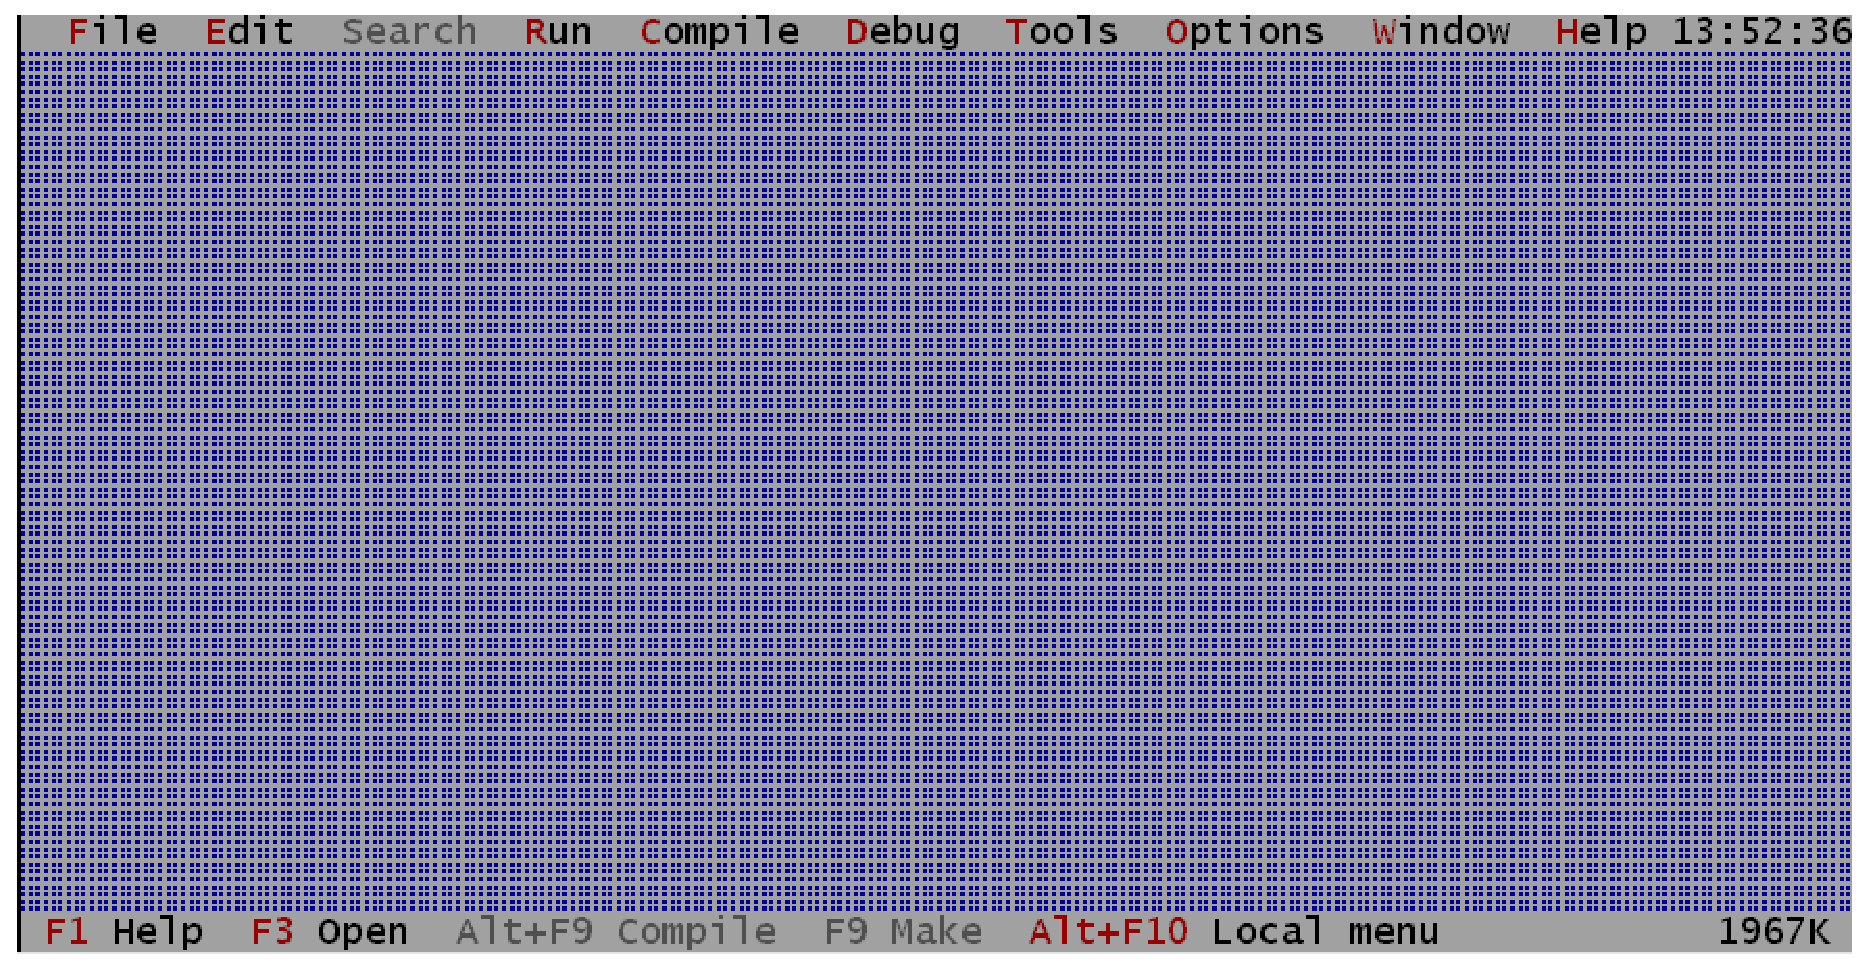
\epsfig{file=pics/idestart.png,width=\textwidth}
\else
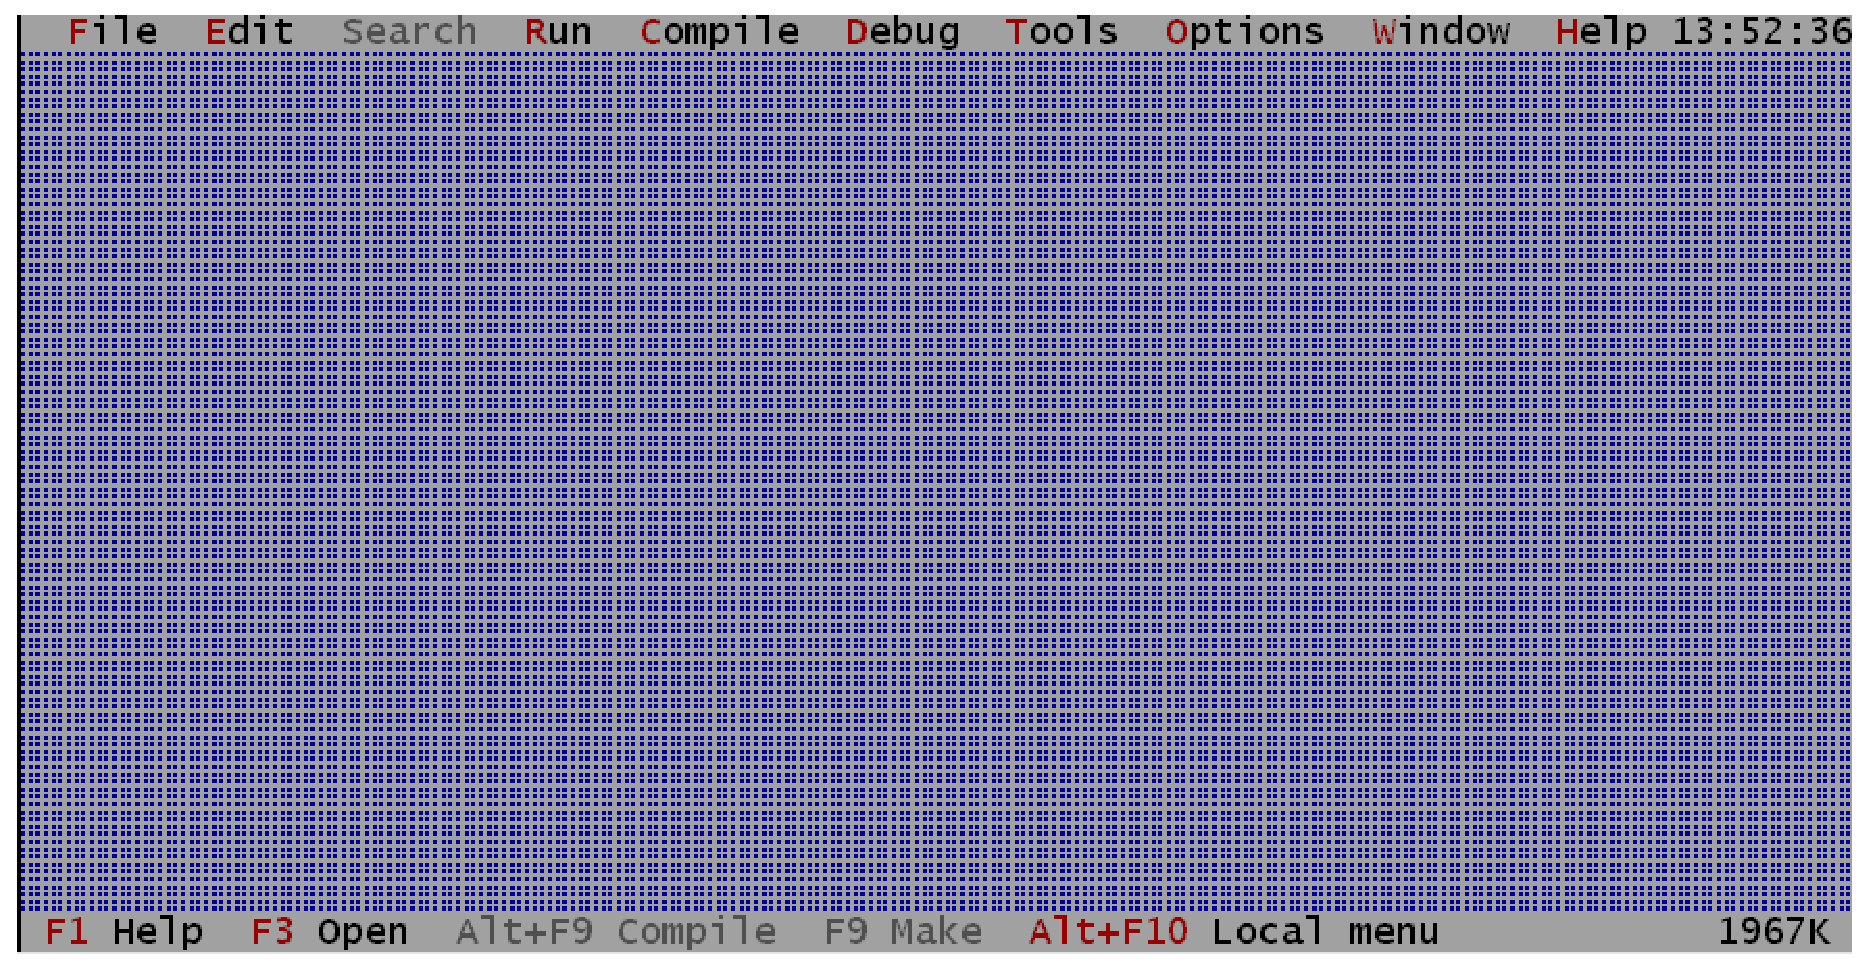
\epsfig{file=pics/idestart.eps,width=\textwidth}
\fi
\end{figure}
\end{latexonly}
At top of the screen the \emph{menu bar} is visible, at the bottom
the \emph{status bar}. The empty space between them is called the
\emph{desktop}.

The statusbar shows the keyboard shortcuts for frequently used 
commands, and allows quick access to these commands by clicking 
them with the mouse. 
At the right edge of the statusbar, the current amount of unused 
memory is displayed. This is only an indication, since the IDE 
tries to allocate more memory from the operating system if it 
runs out of memory.

The menu provides access to all of the IDE's functionality, and
at the right edge of the menu, a clock is displayed.

The IDE can be left by selecting \var{File|Exit} in the menu
\footnote{\var{File|Exit} means select the item Exit in the menu File}
or by pressing \key{Alt-X}.

%%%%%%%%%%%%%%%%%%%%%%%%%%%%%%%%%%%%%%%%%%%%%%%%%%%%%%%%%%%%%%%%%%%%%%%
% Navigating in the IDE
\section{Navigating in the IDE}
The IDE can be navigated both with the keyboard and with a mouse, if your
system has a mouse.

\subsection{Using the keyboard} 
All functionality of the IDE is available through use of the keyboard.
\begin{itemize}
\item It is used for typing and navigating through the sources.
\item Editing commands such as copying and pasting text.
\item Moving and resizing windows.
\item It can be used to access the menu, by pressing \key{ALT} and the
appropriate highlighted menu letter, or by pressing \key{F10} and
navigating through the menu with the arrow keys.

more information on the menu can be found in \sees{idemenu}
\item Many commands in the IDE are bound to shortcuts, i.e. typing a special
combination of keys will execute a command immediatly.
\end{itemize}
\begin{remark}
A complete reference of all keyboard shortcuts can be found in
\sees{keyshortcuts}.
\end{remark}

\subsection{Using the mouse}
\label{suse:mouseusage}
If the system is equipped with a mouse, it can be used to work with the
IDE. The left button is used to select menu items, press buttons, select
text blocks etc. 

The right mouse button is used to access the local menu, if
it is available. Holding down the \key{Ctrl} or \key{Alt} key and 
clicking the right button will execute user defined functions, 
see \sees{prefmouse}.

\begin{remark}
\begin{enumerate}
\item Occasionally, the manual uses the term "drag the mouse". This
means that the mouse is moved while the left mouse button is being 
pressed.
\item 
The action of mouse buttens may be reversed, i.e. the actions of the left
mouse button can be assigned to the right mouse button and vice versa  
\footnote{See \sees{prefmouse} for more information on how to reverse the
actions of the mouse buttons.}. Throughout the manual, it is assumed 
that the actions of the mouse buttons are not reversed.
\item
The mouse is not allways available, even if a mouse is installed:
\begin{itemize}
\item The IDE is running under \linux throught a telnet connection from 
a \windows machine.
\item The IDE is running under \linux in an X-term under X-windows.
\end{itemize}
\end{enumerate}
\end{remark}

%%%%%%%%%%%%%%%%%%%%%%%%%%%%%%%%%%%%%%%%%%%%%%%%%%%%%%%%%%%%%%%%%%%%%%%
% Windows
\section{Windows}
\label{se:windows}
Nowadays, working with windowed applications should be no problem for
most \windows and \linux users. Nevertheless, the following section 
describes how the windows work in the \fpc IDE, to allow efficient 
work with it.
%
% Window basics
%
\subsection{Window basics}
\label{se:windowbasics}
\begin{htmlonly}
A common IDE window is displayed  below:
\htmladdimg{../pics/idewin.gif}
\end{htmlonly}
\begin{latexonly}
A common IDE window is displayed in figure \ref{fig:idewin}.
\begin{figure}
\caption{A common IDE window}
\label{fig:idewin}
\ifpdf
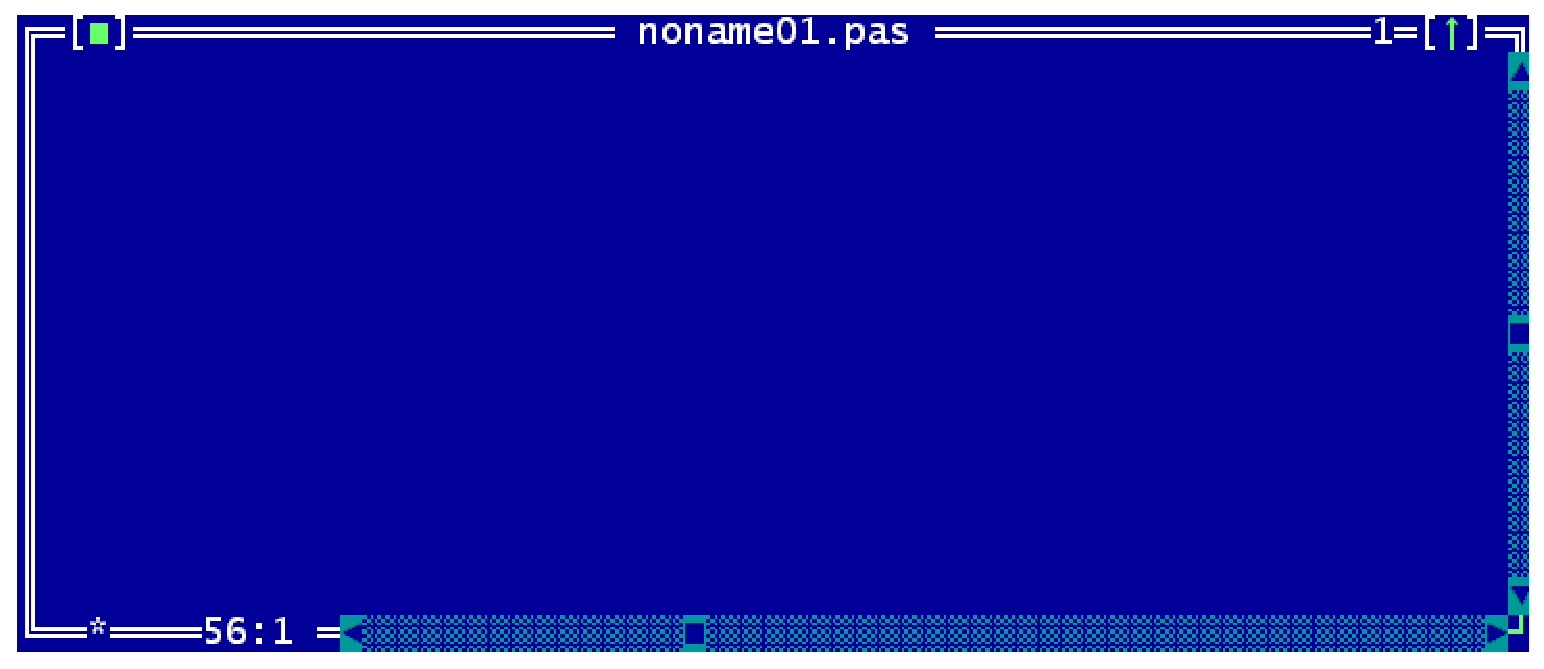
\epsfig{file=pics/idewin.png,width=\textwidth}
\else
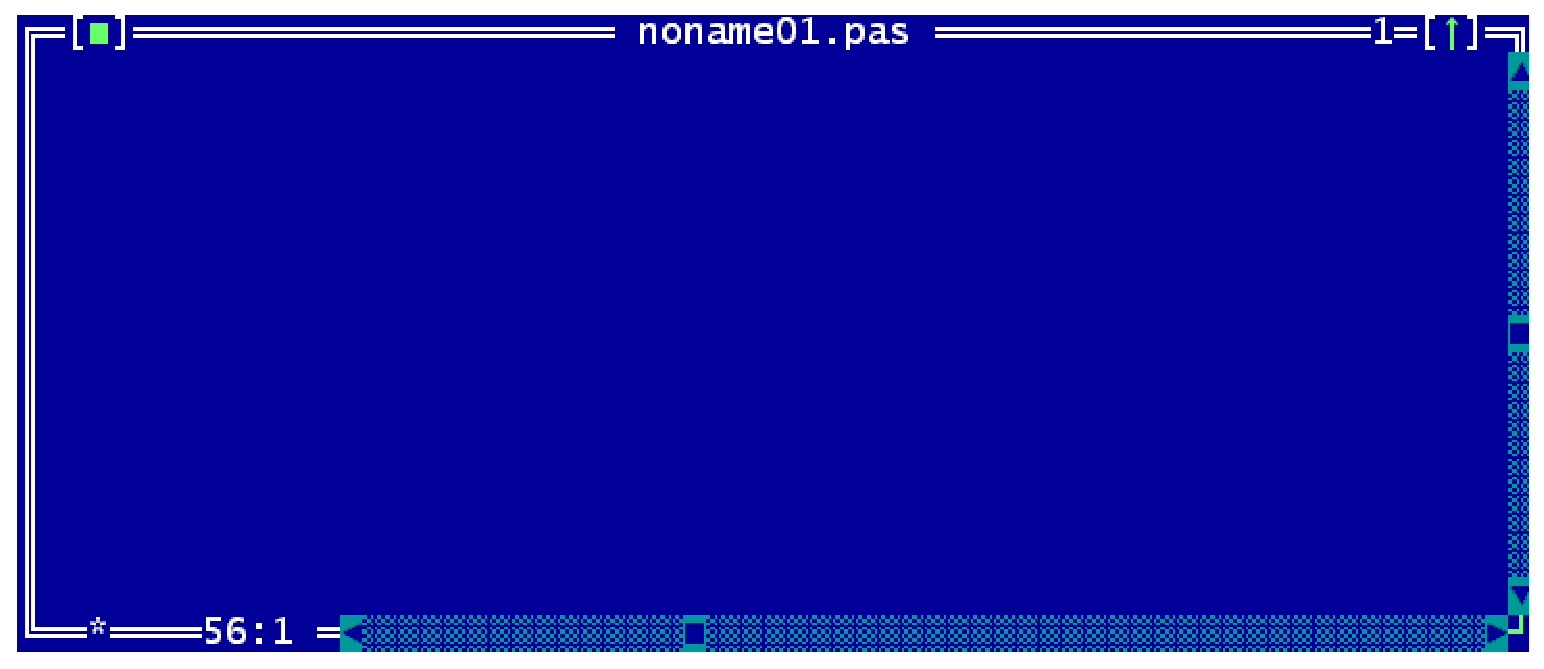
\epsfig{file=pics/idewin.eps,width=\textwidth}
\fi
\end{figure}
\end{latexonly}
The window is surrounded by a so-called \emph{frame}, the white double
line around the window. 

At the top of the window 3 things are displayed:
\begin{itemize}
\item 
At the upper left corner of the window, a \emph{close icon} is shown. 
When clicked, the window will be closed. It can be also closed by
 pressing \key{Alt-F3} or selecting the menu item \var{Window|Close}. 
All open windows can be closed by selecting the menu item 
\var{Window|Close all}.
\item In the middle, the title of the window is displayed.
\item At the upper right corner, a small green arrow is visible.
Clicking this arrow zooms the window so it covers the whole desktop. 
Clicking this arrow on a zoomed window will restore old size of the 
window. Pressing the key \key{F5} has the same effect as clicking 
that arrow. The same effect can be achieved with the menu item \var{Window|Zoom}.
Windows and dialogs which aren't resizeable can't be zoomed, either.
\end{itemize}

The right edge and bottom edges of a window contain scrollbars.
They can be used to scroll the window contents with the mouse. 
The arrows at the ends of the scrollbars can be clicked to scroll the 
contents line by line. Clicking on the dotted area between the arrows 
and the cyan-coloured rectangle will scroll the window's content 
page by page. By dragging the rectangle the content can be scrolled 
continuously.

The star and the numbers in the lower left corner of the window
display information about the contents of the window. They
are explained in the section about the editor, see \sees{editingtext}.

%
% Sizing+moving windows
%
\subsection{Sizing and moving windows}
\label{se:windowsizingmoving}
A window can be moved and sized using the mouse and the keyboard:
To move a window, either:
\begin{itemize}
\item using the mouse, click on the title bar and drag the window 
with the mouse.
\item using the keyboard, go into the size/move mode
by pressing \key{Ctrl-F5} or selecting the menu item
\var{Window|Size/Move}. . Using the cursor keys the window can be moved. 
The size/move mode can be left by pressing \key{Enter}. 
In this case, the window will keep its size and position. 
Alternativly, pressing \key{Esc} will restore the old position.
\end{itemize} 
To resize a window, either:
\begin{itemize}
\item using the mouse, click on the lower right corner of the window
and drag it.
\item using the keyboard, go into the size/move mode
by pressing \key{Ctrl-F5} or selecting the menu item
\var{Window|Size/Move}. The window frame will be green to indicate that
the IDE is in size/move mode. 
By pressing shift and the cursor keys simultaneously, the window can 
be resized.  The size/move mode can be left by pressing
\key{Enter}. In this case, the window will keep the new size.
Pressing \key{Esc} will restore the old size.
\end{itemize}
Not all windows can be resized. This applies, for example, to
\emph{dialog windows} (\sees{dialogwindow}).

A window can also be hidden. To hide a window, the \key{Ctrl-F6} key
combination can be used, or the \var{Window|Hide} menu may be selected.
To restore a Hidden window, it is necessary to select it from the window
list. More information about the window list can be found in the next
section.   
%
% Multiple windows
%
\subsection{Working with multiple windows}
\label{se:multiplewindows}
When working with larger projects, it is likely that multiple windows 
will appear on the desktop. However, only one of these windows will be 
the active window, all other windows will be inactive.

An inactive window is identified by a grey frame. An inactive window can
be made active in one of several ways:
\begin{itemize}
\item using the mouse, activate a window by clicking on it.
\item using the keyboard, pressing \key{F6} will step trough all open 
windows. To activate the previously activated window, \key{Shift-F6} can
be used.
\item the menu item \var{Window|Next} can be used to activate the next 
window in the list of windows, while \var{Window|Previous} will select
the previous window.
\item If the window has a number in the upper right corner, it can be
activated by pressing \key{Alt-<number>}.
\item Pressing \key{Alt-0} will pop up a dialog with a lis  with all 
available windows which allows a quick activation of windows which 
don't have a number.
\end{itemize}

The windows can be ordered and placed on the IDE desktop by zooming and
resizing them with the mouse or keyboard. This is a tyime-consuming task, 
and particularly difficult with the keyboard. Instead, the menu items
\var{Window|Tile} and \var{Window|Cascade} can be used:
\begin{description}
\item[Tile] will divide whole desktop space evenly between all resizable 
windows. 
\item[Cascade] puts all windows in a cascaded position. 
\end{description}

In very rare cases the screen of the IDE may be mixed up. In this
case the whole IDE screen can be refreshed by selecting the menu item 
\var{Window|Refresh display}.
%
% Dialog windows
%
\subsection{Dialog windows}
\label{se:dialogwindow}
In many cases the IDE displays a dialog window to get user input.
The main difference to normal windows is that other windows cannot be
activated while a dialog is active. Also the menu is not accessible while in
a dialog. This behavior is called \emph{modal}. To activate another window, 
the modal window or dialog must be closed first.

\begin{htmlonly}
A typical dialog window looks like:
\htmladdimg{../pics/idedlg.gif}
\end{htmlonly}
\begin{latexonly}
Figure \ref{fig:idedlg} shows a typical dialog window.
\begin{figure}
\caption{A typical dialog window}
\label{fig:idedlg}
\ifpdf
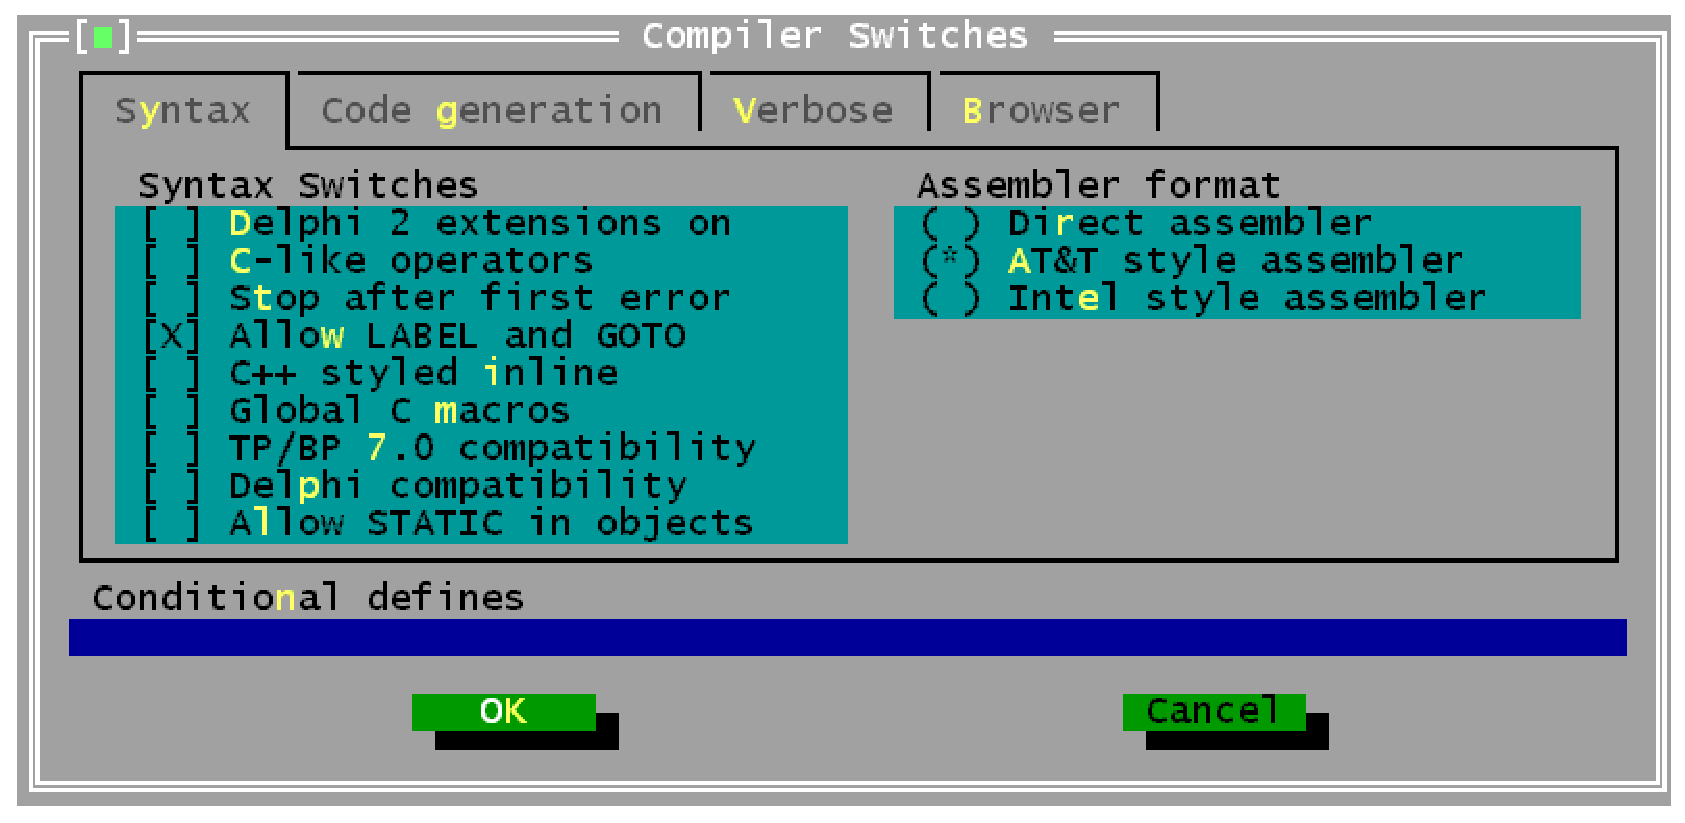
\epsfig{file=pics/idedlg.png,width=\textwidth}
\else
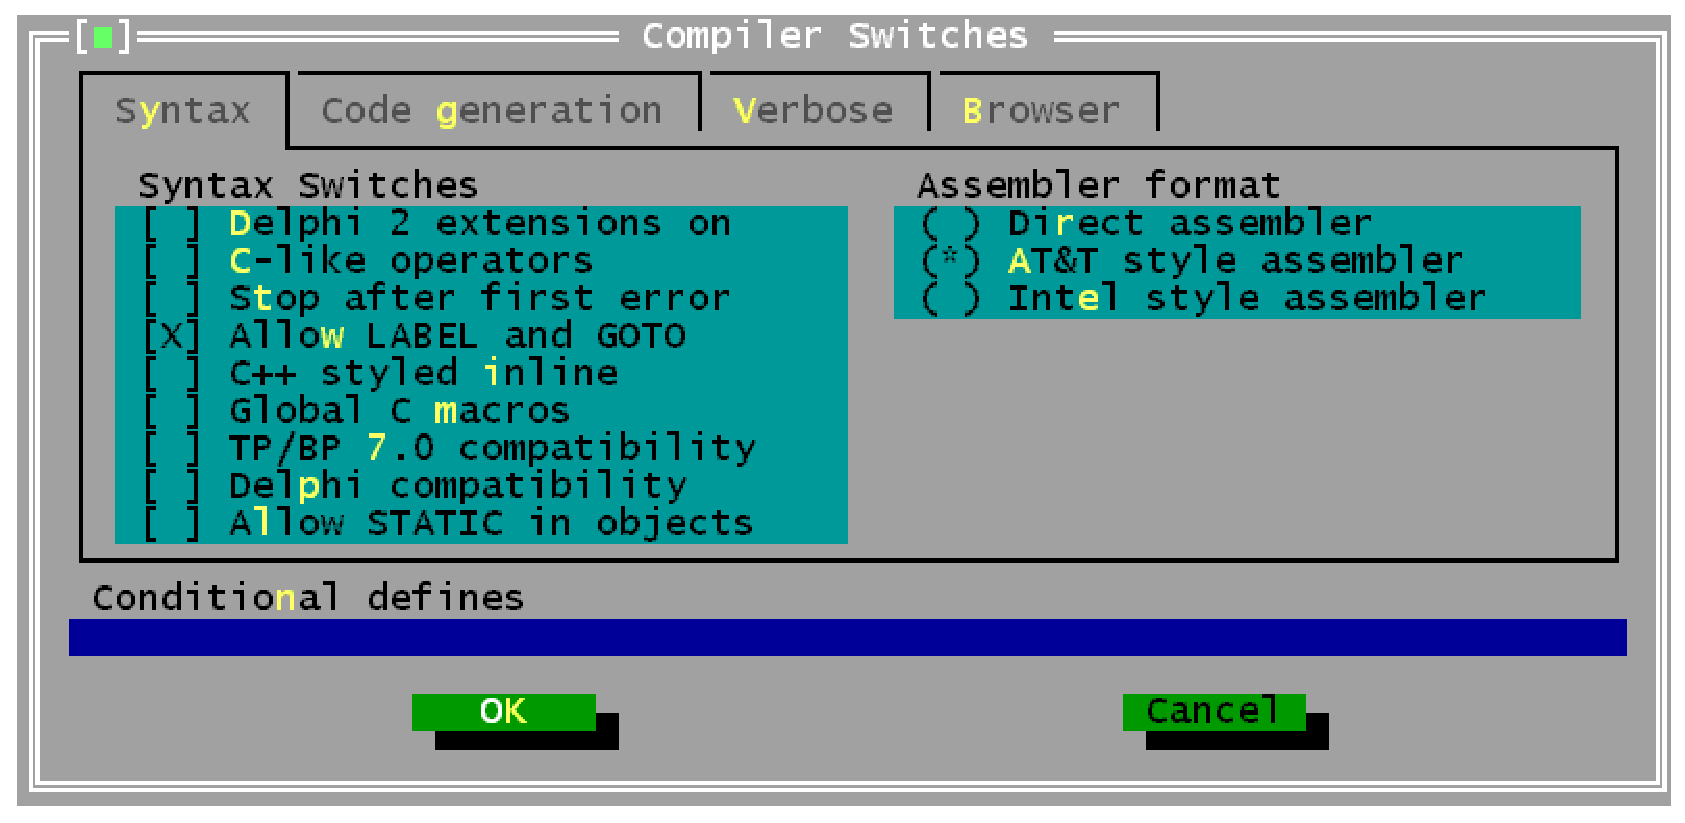
\epsfig{file=pics/idedlg.eps,width=\textwidth}
\fi
\end{figure}
\end{latexonly}

%%%%%%%%%%%%%%%%%%%%%%%%%%%%%%%%%%%%%%%%%%%%%%%%%%%%%%%%%%%%%%%%%%%%%%%
% The menu
\section{The Menu}
\label{se:idemenu}
The main menu (the gray bar at the top of the IDE) provides access to all the
functionality of the IDE. It also displays a clock, displaying the current
time. The menu is always available, except when a dialog is opened. If a
dialog is opened, it must be closed first in order to access the menu.

In certain windows, a local menu is also available. The local menu will
appear where the cursor is, and provides additional commands that are 
context-sensitive.
%
% Accessing the menu
%
\subsection{Accessing the menu}
The menu can be accessed in a number of ways:
\begin{enumerate}
\item By using the mouse to select items. The mouse cursor should be located
over the desired menu item, and a left mouse click will then select it.
\item By pressing \key{F10}. This will switch the IDE focus to the menu. 
Use the arrow keys can then be used to navigate in the menu, the 
\key{Enter} key should be used to select items.
\item To access menu items directly, \key{Alt-<highlighted menu letter>}
can be used to select a menu item. Afterwards submenu entries can be selected 
by pressing the highlighted letter, but without \key{Alt}. 
E.g. \key{Alt-S G} is a fast way to display the \emph{goto line} dialog.
\end{enumerate}
Every menu item is explained by a short text in the status bar.

When a local menu is available, it can be accessed by pressing
the right mouse button or \key{Alt-F10}. 

In the subsequent, all menu entries and their actions are described.
%
% The file menu
%
\subsection{The File menu}
\label{se:menufile}
\begin{description}
\item[New] Opens a new, empty editor window. 
\item[New from template] Prompts for a template to be used, asks to fill in
any parameters, and then starts a new editor window with the template.
\item[Open] (\key{F3}) Presents a file selection dialog, and opens 
the selected file in a new editor window. 
\item[Save] (\key{F2}) Saves the contents of the current edit window 
with the current filename. If the current edit window does not yet have
a filename, a dialog is presented to enter a filename.
\item[Save as] Presents a dialog in which a filename can be entered. The
current window's contents are then saved to this new filename, and the
filename is stored for further save actions.
\item[Change dir] Presents a dialog in which a directory can be selected.
The current working directory is then changed to the selected directory.
\item[Dos shell] executes a command shell. After the shell exited, the
IDE resumes.
\item[Exit] (\key{ALT-X}) Exits the IDE. If any unsaved files are 
in the editor, the IDE will ask if these files should be saved.
\end{description}
%
% The edit menu
%
\subsection{The Edit menu}
\label{se:menuedit}
\begin{description}
\item[Undo] (\key{ALT-BkSP})
Undo the last editing action. The editing actions are stored in a buffer,
selecting this mechanism will move backwards through this buffer, i.e.
multiple undo levels are possible.
\item[Redo] Redo the last action that was previously undone. Redo can redo
multiple undone actions. 
\item[Dump undo]
Clears the undo buffer. After this action, the undo and redo menu will be 
unavailable till new editing actions have taken place.
\item[Undo all]
Undo all actions in the undo buffer. If a new empty file was started, this
action should clear the window contents again.
\item[Redo all]
Redo all editing actions that were undone.
\item[Cut] (\key{Shift-DEL}) Copy the current selection to the clipboard
and delete the selection from the text. Any previous clipboard contents is
lost after this action. After this action, the clipboard contents can be 
pasted elsewhere in the text.
\item[Copy] (\key{Ctrl-INS}) Copy the current selection to the clipboard.
Any previous clipboard contents is lost after this action. 
After this action, the clipboard contents can be pasted elsewhere in the text.
\item[Paste] (\key{Shift-INS}) Insert the current clipboard contents in
the text at the cursor position. The clipboard contents remains as it was.
\item[Clear] (\key{Ctrl-DEL}) clears (i.e. deletes) the current
selection.
\item[Show clipboard] Opens a window in which the current clipboard contents
is shown.
\end{description}
%
% The Search menu
%
\subsection{The Search menu}
\label{se:menusearch}
\begin{description}
\item[Find] (\key{Ctrl-Q F}) presents the search dialog. A search text 
can be entered, and when the dialog is closed, the entered text is searched
in the active window. If the text is found, it will be selected. 
\item[Replace] (\key{Ctrl-Q A} presents the search and replace dialog.
After the dialog is closed, the search text will be replaced by the replace
text in the active window.
\item[Search again] (\key{CTRL-L}) repeats the last search or search and replace action,
 using  the same parameters.
\item[Go to line number] (\key{Alt-G}) prompts for a line number, and
then jumps to this line number.
\item[Find procedure]
Not yet implemented.
\item[Objects]
Not yet implemented.
\item[Modules]
Not yet implemented.
\item[Globals]
Not yet implemented.
\item[Symbol]
Not yet implemented.
\end{description}
%
% The Run menu
%
\subsection{The Run menu}
\label{se:menurun}
\begin{description}
\item[Run] (\key{Ctrl-F9})
If the sources were modified, compile the program. If the compile is
successful, the program is executed. If the primary file  was set, then 
that is used to determine which program to execute. See \sees{menucompile}
for more information on how to set the primary file.
\item[Step over] (\key{F8})
Run the program till the next source line is reached. If any calls to 
procedures are made, these will be executed completely as well.
\item[Trace into] (\key{F7})
Execute the current line. If the current line contains a call to another
procedure, the process will stop at the entry point of the called procedure.
\item[Goto cursor] (\key{F4})
Runs the program till the execution point matches the line where the cursor
is.
\item[until return]
Runs the current procedure till it exits.
\item[parameters]
This menu item allows to enter parameters that will be passed on to the
program when it is being executed.
\item[program reset] (\key{Ctrl-F2}) if the program is being run or 
debugged, the debug session is aborted, and the running program is killed.
\end{description}
%
% The compile menu
%
\subsection{The Compile menu}
\label{se:menucompile}
\begin{description}
\item[Compile] (\key{Alt-F9}) Compiles the contents of the active window.  
If the primary file was set, the primary file is compiled instead.
\item[Make] (\key{F9}) Compiles the contents of the active window, and
any files that the unit or program depends on and that were modified since
the last compile.
If the primary file was set, the primary file is compiled instead.
\item[Build]
Compiles the contents of the active window, and any files that the unit or 
program depends on, whether they were modified or not.
If the primary file was set, the primary file is compiled instead.
\item[Target] Sets the target operating system for which should be compiled. 
\item[Primary file] Sets the primary file. If set, any run or compile command 
will act on the primary file instead of on the active window. The primary
file need not be loaded in the IDE for this to have effect.
\item[Clear primary file]
Clears the primary file. After this command, any run or compile action will
act on the active window.
\item[Information] Displays some information about the current program.
\item[Compiler messages] (\key{F12}) displays the compiler messages
window. This window will display the messages generated by the compiler
during the last compile.
\end{description}
%
% The debug menu
%
\subsection{The Debug menu}
\label{se:menudebug}
\begin{description}
\item[Output]
\item[User screen] (\key{Alt-F5}) switches to the screen as it was last
left by the running program.
\item[Breakpoint] (\key{Ctrl-F8})
Sets a breakpoint at the current line. When debugging, program execution
will stop at this breakpoint.
\item[Call stack] (\key{Ctrl-F3})
Shows the call stack. The call stack is the list of addresses (and
filenames and line numbers, if this information was compiled in) of 
procedures that are currently being called in the running program.
\item[Registers]
Shows the current content of the CPU registers. 
\item[Add watch] (\key{Ctrl-F7}) Add a watch. A watch is an expression
that can be evaluated by the IDE and shown in a special window. usually this
is the contents of some variable. 
\item[Watches]
Shows the current list of watches in a separate window.
\item[Breakpoint list]
Shows the current list of breakpoints in a separate window.
\item[GDB window]
Shows the GDB debugger console. This can be used to interact with the debugger
directly.
\end{description}
%
% The tools menu
%
\subsection{The Tools menu}
\label{se:menutools}
\begin{description}
\item[Messages] (\key{F11}) Show the messages window. 
This window contains the output from one of the tools. For more information,
see \sees{toolsmessages}.
\item[Goto next] (\key{Alt-F8}) goto next message.
\item[Goto previous] (\key{Alt-F7}) goto previous message
\item[Grep] (\key{SHIFT-F2}) Prompts for a regular expression and options
to be given to grep, and then executes \file{grep} with the given expression and
options. For this to work, the \file{grep} program must be installed on your
system, and be in a directory that is in the \var{PATH}. For more
information, see \sees{grep}.
\item[Calculator] 
Displays the calculator. For more information, see \sees{calculator}
\item[Ascii table] Displays the \var{ASCII} table. For more information, see
\sees{asciitable}
\end{description}
%
% The Search menu
%
\subsection{The Options menu}
\label{se:menuoptions}
\begin{description}
\item[Mode] Presents a dialog to set the current mode of the compiler. The
current mode is shown at the right of the menu entry. For more information,
see \sees{compilermode}.
\item[Compiler] Presents a dialog that can be used to set common compiler
options. These options will be used when compiling a program or unit.
\item[Memory sizes]
Presents a dialog where the stack size and the heap size for the program can
be set. These options will be used when compiling a program.
\item[Linker]
Presents a dialog where some linker options can be set. These options will
be used when a program or library is compiled.
\item[Debugger]
Presents a dialog where the debugging options can be stored. These options
are used when compiling units or programs. Note that the debugger will not
work unless debugging information is generated in the program.
\item[Directories]
Presents a dialog where the various directories needed by the compiler can
be set. These directories will be used when a program or unit is compiled.
\item[Browser]
Presents a dialog where the browser options can be set. The browser options
affect the behaviour of the symbol browser of the IDE. 
\item[Tools]
Presents a dialog to configure the tools menu. For more information, see
\sees{addingtools}.
\item[Environment]
Presents a dialog to configure the behaviour of the IDE. A sub menu is
presented with the various aspects of the IDE:
\begin{description}
\item[Preferences]
General preferences, such as whether to save files or not, and which files
should be saved. The video mode can also be set here.
\item[Editor]
Controls various aspects of the edit windows.
\item[CodeComplete]
Used to set the words which can be automatically completed when typing in
the editor windows.
\item[Codetemplates]
Used to define code templates, which can be inserted in an edit window.
\item[Desktop]
Used to control the behaviour of the desktop, i.e. several features can be
switched on or off.
\item[Mouse]
Can be used to control the actions of the mouse, and to assign commands to
various mouse actions.
\item[Startup]
Not yet implemented.
\item[Colors]
Here the various colors used in the IDE and the editor windows can be set.
\end{description}
\item[Open]
Presents a dialog in which a file with editor preferences can be selected. 
after the dialog is closed, the preferences file will be read and the
preferences will be applied.
\item[Save]
Save the current options in the default file.
\item[Save as]
Saves the current options in an alternate file. A file selection dialog box
will be presented in which the alternate settings file can be entered.
\end{description}
%
% The window menu
%
\subsection{The Window menu}
\label{se:menuwindow}
The Window menu provides access to some window functions. More information
on all these functions can be found in \sees{windows}
\begin{description}
\item[Tile]
Tiles all opened windows on the desktop.
\item[Cascade]
Cascades all opened windows on the desktop.
\item[Close all]
Close all opened windows.
\item[Size/move] (\key{Ctrl-F5})
Put the IDE in Size/move modus; after this command the active window can be
moved and resized using the arrow keys.
\item[Zoom] (\key{F5})
Zooms or unzooms the current window. 
\item[Next] (\key{F6})
Activates the next window in the window list.
\item[Previous] (\key{SHIFT-F6})
Activates the previous window in the window list.
\item[Hide] (\key{Ctrl-F6})
Hides the active window. 
\item[Close] (\key{ALT-F3}) closes the active window.
\item[List] (\key{Alt-0}) shows the list of opened windows. From there a
window can be activated, closed, shown and hidden.
\item[Refresh display]
Redraws the screen.
\end{description}
%
% The Help menu
%
\subsection{The Help menu}
\label{se:menuhelp}
\begin{description}
\item[Contents]
Shows the help table of contents
\item[Index] (SHIFT-F1)
Jumps to the help Index.
\item[Topic search]  (CTRL-F1)
Jumps to the topic associated with the currently highlighted text.
\item[Previous topic] (ALT-F1)
Jumps to the previously visited topic.
\item[Using help]
Displays help on using the help system.
\item[Files]
Allows to configure the help menu. Here help files can be added to the help
system.
\item[About]
Displays information about the IDE. See \sees{about} for more information.
\end{description}

%%%%%%%%%%%%%%%%%%%%%%%%%%%%%%%%%%%%%%%%%%%%%%%%%%%%%%%%%%%%%%%%%%%%%%%
% The help system
\section{The help system}
More information on how to handle the IDE, or about the use of various
calls in the RTL, explanations regarding the syntax of a pascal statement,
can be found in the \emph{help system}. The help system is activated
 by pressing F1.

\subsection{Navigating in the help system}
The help system contains hyperlinks which can be accessed by clicking
them with the mouse. Alternativly, \key{Tab} and \key{Shift-Tab}
can be used to move between the different hyperlinks of a page
and the \key{Enter} key can be used to select them.

The contents of the help system is displayed, if \key{Shift-F1} is
pressed. To go back to the last help topic, \key{press Alt-F1}. 
This also works if the help window isn't displayed on the desktop.

\subsection{Working with help files}
The IDE contains a help system which can display HTML files
as well as the TPH format known from \tp. The HTML viewer of the 
help system is limited, it can only handle the most basic HTML files 
not including graphics, since it is only designed to display the \fpc help 
files \footnote{...but feel free to improve it and send patches to the 
\fpc development team...}.

The menu item \var{Help|Files} permits you to add and delete
help files.

A new file can be added with the \emph{new} button. The IDE will display
a prompt, in which the location of the help file should be entered.
If it is an HTML file, a dialog box will be displayed
which asks for a title. This title will then be included in the
contents of help.

A help file can be deleted from the help system (it is \emph{not} deleted 
from the hard disk) using the \emph{delete} button.

\subsection{The about dialog}
\label{se:about}
The \emph{about dialog} (\var{Help|About...}) shows some information
about the IDE, such as the version number, the date it was built, what
compiler and debugger it uses. When reporting bugs about the IDE, please 
It also contains copyright information.

%%%%%%%%%%%%%%%%%%%%%%%%%%%%%%%%%%%%%%%%%%%%%%%%%%%%%%%%%%%%%%%%%%%%%%%
% Editing text
\section{Editing text}
\label{se:editingtext}
In this section, the basics of editing (source) text are explained. The IDE
works like many other text editors in this respect, so mainly the
distinguishing points of the IDE will be explained.

\subsection{Insert modes}
Standard, the IDE is in insert mode. This means that any text that is typed
will be inserted before text that is present after the cursor. 

In overwrite mode, any text that is typed will replace existing text. 

When in insert mode, the cursor is a flat blinking line. If the IDE is in
overwrite, the cursor is a cube with the height of one line.
%
% blocks
%
\subsection{Blocks}
\label{se:blocks}
The IDE handles selected text just as the \tp IDE handles it. This is
slightly different from the way e.g. Windows applications handle selected
text. 

Text can be selected in 3 ways:
\begin{enumerate}
\item using the mouse, dragging the mouse over existing text selects it.
\item using the keyboard, press \key{Ctrl-K B} to mark the beginning of
the selected text, and \key{Ctrl-K K} to mark the end of the selected
text.
\item using the keyboard, hold the \key{Shift} key depressed while
navigating with the cursor keys.
\end{enumerate}

There are also some special select commands:
\begin{enumerate}
\item The current line can be selected using \key{Ctrl-K L}.
\item The current word can be selected using \key{Ctrl-K T}.
\end{enumerate}

In the \fpc IDE, selected text is persistent. After selecting a range of 
text, the cursor can be moved, and the selection will not be destroyed;
hence the term 'block' is more appropriate for the selection, and will be
used henceforth...

Several commands can be executed on a block:
\begin{itemize}
\item Move the block to a new location (\key{Ctrl-K V}).
\item Copy the block to another location (\key{Ctrl-K C}).
\item Delete the block (\key{Ctrl-K Y}).
\item Write the block to a file (\key{Ctrl-K W}).
\item Read the contents of a file into a block (\key{Ctrl-K R}).
\item Indent a block (\key{Ctrl-K I}).
\item Undent a block (\key{Ctrl-K U}).
\item Print the block contents (\key{Ctrl-K P}).
\item Restrict a search to the block contents.
\end{itemize}

%
% Bookmarks
%
\subsection{Setting bookmarks}
\label{se:bookmarks}
The IDE provides a feature which allows to set a bookmark at the current 
cursor position. Later, the cursor can be returned to this position 
by pressing a keyboard shortcut.

Up to 9 bookmarks per source file can be set up, they are set by
\key{Ctrl-K <Number>} (where number is the number of the mark).
To go to a previously set bookmark, press \key{Ctrl-Q <Number>}.

\begin{remark}
Currently, the bookmarks are not stored if the IDE is left. This may
change in future implementations of the IDE.
\end{remark}

%%%%%%%%%%%%%%%%%%%%%%%%%%%%%%%%%%%%%%%%%%%%%%%%%%%%%%%%%%%%%%%%%%%%%%%
% Searching in the text
\section{Searching and replacing}
\label{se:searching}
The IDE allows to search for text in the active editor window. 
To search for text, one  of the following can be done:
\begin{enumerate}
\item Select "Search|Find" in the menu.
\item Press \key{Ctrl-Q F}.
\end{enumerate}
After that, a dialog will pop up in which you can enter the following
options:
\begin{description}
\item[Text to find] the text to be searched for. If a block was active when
the dialog was started, this is proposed.
\item[Case sensitive] when checked, the search is case sensitive.
\item[Whole words only] when checked, the search text must appear in the
text as a complete word.
\item[Direction] the direction in which the search must be conducted,
starting from the specified origin.
\item[Scope] should the search be on the whole file, or just the selected
text.
\item[Origin] should the search start from the cursor position or the start
of the scope.
\end{description}
After the dialog is closed, the search is performed using the given options.

A search can be repeated (using the same options) in one of 2 ways:
\begin{enumerate}
\item Select "Search|Find again" from the menu.
\item Press \key{Ctrl-L}.
\end{enumerate}

It is also possible to replace occurences of a text with another text. 
This can be done in a similar manner to searching for a text:
\begin{enumerate}
\item Select "Search|Replace" from the menu.
\item Press \key{Ctrl-Q A}.
\end{enumerate}
A dialog, similar to the search dialog will pop up.
In this dialog, in addition to the things that can be filled in in the
search dialog, the following things can be entered:
\begin{description}
\item [New text] text by which found text will be replaced.
\item [Prompt on replace] before a replacement is made, the IDE will ask for
confirmation.
\end{description}
If the dialog is closed with the 'OK' button, only the next occurrence the
the search text will be replaced. 
If the dialog is closed with the 'Change All' button, all occurrences of 
the search text will be replaced.

\subsection{The symbol browser}
\label{se:browser}
The symbol browser allows to find all occurrences of a symbol. A symbol 
can be a variable, type, procedure or constant that occurs in your program.

To enable the symbol browser, the program or unit must be compiled with
browser information. This can be done by setting the browser information
option in the compiler options dialog.

The IDE allows to browse several types of symbol:
\begin{description}
\item[procedures] Allows to quickly jump to a procedure definition or
implementation.
\item[Objects] Allows to quickly browse an object.
\item[Modules] Allows to browse a module.
\item[Globals] Allows to browse any global symbol.
\item[Arbitrary symbol] Allows to browse an arbitrary symbol.
\end{description}
In all cases, first a symbol to be browsed must be selected. After that,
a browse window appears. In the browse window, all locations where the 
symbol was encountered are shown. Selecting a location and pressing the
space bar will cause the editor to jump to that location; the line
containing the symbol will be highlighted. 

If the location is in a source file that is not yet displayed, a new 
window will be opened with the source file loaded.

After the desired location was reached, the browse window can be closed 
with the usual commands. 

%%%%%%%%%%%%%%%%%%%%%%%%%%%%%%%%%%%%%%%%%%%%%%%%%%%%%%%%%%%%%%%%%%%%%%%
% Running programs
\section{Running programs}
\label{se:running}
A compiled program can be run straight from the IDE. This can be done
in one of several ways:
\begin{enumerate}
\item select the "Run|Run" menu, or
\item press \key{Ctrl-F9}.
\end{enumerate}
If command-line parameters should be passed to the program, then these
can be set through the "Run|Parameters" menu. 
\begin{htmlonly}
The Parameters dialog.
\htmladdimg{../pics/ide/params.png}
\end{htmlonly}
\begin{latexonly}
\begin{figure}[h]
\caption{The program parameters dialog.}
\label{fig:ides}
\ifpdf
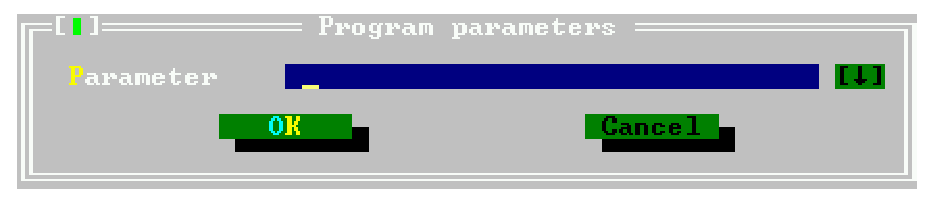
\epsfig{file=pics/ide/params.png,width=\textwidth}
\else
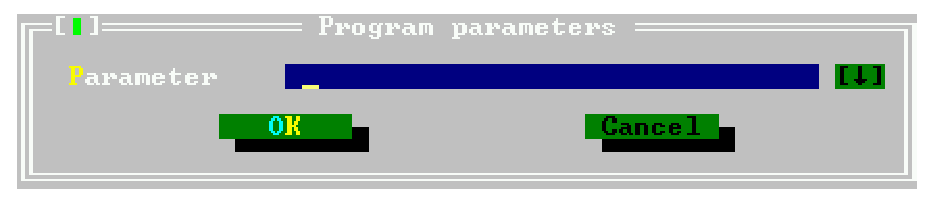
\epsfig{file=pics/ide/params.eps,width=\textwidth}
\fi
\end{figure}
\end{latexonly}

Once the program started, it will continue to run, until 
\begin{enumerate}
\item the program quits normally,
\item an error happens,
\item A breakpoint is encountered.
\end{enumerate}
The last alternative is only possible if the program is compiled
with debug information.

Alternatively, it is possible to position the cursor somewhere in a
source file, and run the program till the execution reaches the
source-line where the cursor is located. This can be done by
\begin{enumerate}
\item selecting "Run|Goto Cursor" in the menu,
\item pressing \key{F4}.
\end{enumerate}
Again, this is only possible if the program was compiled with debug
information.

The program can also executed line by line. Pressing \key{F8} will 
execute the next line of the program. If the program wasn't started
yet, it is started. Repeatedly pressing \key{F8} will execute line 
by line of the program, and the IDE will show the line to be executed 
in an editor window. If somewhere in the code a call occurs to a subroutine,
then pressing \key{F8} will cause the whole routine to be executed before
control returns to the IDE. If the code of the subroutine should be stepped
through as well, then \key{F7} should be used instead. Using \key{F7} will
cause the IDE to execute line by line of any subroutine that is encountered.

If a subroutine is being stepped through, then the "Run|Until return" menu
will execute the program till the current subroutine ends. 

If the program should be stopped before it quits by itself, then this can be
done by
\begin{enumerate}
\item selecting "Run|Program reset" from the menu, or
\item pressing \key{Ctrl-F2}.
\end{enumerate}
The running program will then be aborted.

%%%%%%%%%%%%%%%%%%%%%%%%%%%%%%%%%%%%%%%%%%%%%%%%%%%%%%%%%%%%%%%%%%%%%%%
% Debugging programs
\section{Debugging programs}
\label{se:debugging}
To debug a program, it must be compiled with debug information. Compiling a
program with debug information allows to:
\begin{enumerate}
\item Execute the program line by line.
\item Run the program till a certain point (a breakpoint)
\item Inspect the contents of variables or memory locations while the
program is running.
\end{enumerate}

\subsection{Using breakpoints}
Breakpoints will cause a running program to stop when the execution
reaches the line where the breakpoint was set. At that moment, control
is returned to the IDE, and it is possible to continue execution.

To set a breakpoint,


%%%%%%%%%%%%%%%%%%%%%%%%%%%%%%%%%%%%%%%%%%%%%%%%%%%%%%%%%%%%%%%%%%%%%%%
% The tools menu
\section{The tools menu}
\label{se:toolsmenu}
The tools menu allows you an easy access to external tools. Further,
it contains two other probaly helpful tools for programmers: an
ascii table and a calculator.

\subsection{The messages window}
\label{se:toolsmessages}
The output of the external utilies is redirected by the IDE and it
will be displayed in the message window. The message window is
displayed automatically, if an external tool was run. The
messages window can be also display manual by the selecting the
menu item \var{Tools|Messages} or by pressing the key \key{F11}.

If the output of the tools contains filenames and line numbers,
you can goto the source line by pressing \key{Enter} or
double clicking the output line. To trace the source, press
\key{Space}. The difference between goto and tracking is that
goto closes the message window while tracking keeps the message
window active and the source file is displayed only in the background.

The algorithm which extracts the file names and line numbers from
the tool output is quite sophisticated, but in some cases it may
fail. In this case, please refer the sources of the IDE.

\subsection{GREP}
\label{se:grep}
One external tool in the Tools menu is already predefined: an
menu item to call the \file{grep} utility (\var{Tools|Grep} or
\key{Shift-F2}). \file{grep} search for a given string in files and
returns the lines which contain the string. The search string can
be even a regular expression (see \sees{regexpr}).

\subsection{The ascii table}
\label{se:asciitable}
The tools menu provides also an ascii table (\var{Tools|Ascii table},
it allows you to lookup ascii codes as well as
inserting chars into the window which was active when calling the
ascii chart. To get the ascii code of a char move the blocking block
cursor on this char or click with the mouse on it. To insert a
char into an editor window, double click it with the mouse
or press \key{Enter} while the cursor is on it.

\subsection{The calculator}
\label{se:calculator}
The calculator allows you to do quickly some calculations. It doesn't
take care of operator precedence, so be careful. For more information
about the supported operations, see table \seet{calculatorcommands}.

\begin{FPCltable}{p{5cm}lll}{Calculator commands}{calculatorcommands}
Operation & Button & Key \\
\hline
Add two numbers & \var{+} & \key{+} \\
Subtract two numbers & \var{\-} & \key{\-} \\
Multiply two numbers & \var{*} & \key{*} \\
Divide two numbers & \var{/} & \key{/} \\
Calculate power & \var{x\^y} & \\
Add the displayed number to the memory & \var{M+} & \\
Subtract the displayed number from the memory & \var{M-} & \\
Move the memory contents to the display & \var{M->} & \\
Move the display contents to the memory & \var{M<-} & \\
Exchange display and memory contents & \var{M<->} & \\
Square the display contents & \var{x\^2} & \\
Calculate the reciproke value & \var{1/x} & \\
Calculate the square root & \var{sqr} & \\
Calulate the natural logarithm &  \var{log} & \\
Delete the last typed digit & \var{<-} & \key{Backspace} \\
Delete the display & \var{C} & \key{C} \\
Change the sign & \var{+\-} & \\
Get result of operation & \var{=} & \key{Enter} \\
Do per cent calculation & \var{\%} & \key{\%}
\end{FPCltable}

\subsection{Adding new tools}
\label{se:addingtools}
%%%!!!!!!!!!!!!!!

\subsection{Meta parameters}
When specifing the command line for the called tool, meta parameters can
be used. Meta parameters are variables and and they are replaced
by it's contents before passing the command line to the tool.

%%%!!!!!!!!!!!!!!
\begin{description}
\item[\$CAP]
\item[\$CAP\_MSG]
\item[\$CAP\_EDIT]
\item[\$COL] replaced by the coloumn of the cursor in the active window
\item[\$CONFIG]
\item[\$DIR]
\item[\$DRIVE]
\item[\$EDNAME]
\item[\$EXENAME]
\item[\$EXT]
\item[\$LINE] replaced by the line number of the cursor in the active window
\item[\$NAME]
\item[\$NAMEEXT]
\item[\$NOSWAP]
\item[\$DRIVE]
\item[\$PROMPT]
\item[\$SAVE]
\item[\$SAVE\_ALL]
\item[\$SAVE\_CUR]
\item[\$SAVE\_PROMPT]
\item[\$WRITEMSG]
\end{description}

\subsection{Building your own tool command line dialog box}
%%%!!!!!!!!!!!!!!

%%%%%%%%%%%%%%%%%%%%%%%%%%%%%%%%%%%%%%%%%%%%%%%%%%%%%%%%%%%%%%%%%%%%%%%
% Project management
\section{Project management}
\label{se:projectmanagement}
Luckily, project mangament in pascal is much easier than with C. The
compiler knows from the source which units, sources etc. it needs.
So the \fpc IDE does not need a full featured project manager like
some C development environments offer. But some things make life easier...

\subsection{The primary file}
\label{se:primaryfile}
Without a primary file the IDE compiles/runs the source of the actived
window when you start your program. If you have specified a primary
file, the IDE compiles/runs always this source, no matter if another
source window is active. Select the menu item \var{Compile|Primary file...}
to get a file dialog where you can enter the primary file. Only the command
\var{Compile|Compile} compiles still the active window, this is usefull
if you have a large project and you want only check the syntax of the
current source.

The menu item \var{Compiler|Clear primary file} restores the default behavior
i.e. the compile and run commands apply to the active window.

\subsection{The switches mode}
\label{se:compilermode}
The IDE allows you to work with three different sets of compiler
switches: Normal, Debug and Release. The different switch
sets can be selected in the \var{Switches Mode} dialog which
is executed by the menu item \var{Options|Mode...}.
Change the switches mode doesn't do any active switch change, i.e.
the debug mode doesn't include debug information automatically,
it just loads another set of switches which were adjusted before
by the user in the compiler or directory dialog.

\subsection{The directory dialog}
In the directory dialog, you've to specify the directories where
the compiler should look for units, library etc, where the
output files should be stored etc. You can specify multiple
directories (except for the output directory) seperated by
semicolon.

\begin{description}
\item Nothing yet !!!!!!!!!!!!!!
\end{description}

\subsection{The target operating system}
The menu item \var{Compile|Target} allows you to specify the target
operating system. Changing the target doesn't affect any compiler
switches or directories.

\subsection{The configuration files}
%%%!!!!!!!!!!!!!!

%%%%%%%%%%%%%%%%%%%%%%%%%%%%%%%%%%%%%%%%%%%%%%%%%%%%%%%%%%%%%%%%%%%%%%%
% Customize the IDE
\section{Customize the IDE}
The IDE is configurable in a wide range, you can change colors, screen
resolution etc. The configuration setting can reached via the
submenu \var{Environment} in the \var{Options} menu.

\subsection{Preferences}
The \emph{preferences dialog} is called by the menu item
\var{Options|Environment|Preferences}.

%%%!!!!!!!!!!!!!!

\subsubsection{Video modes}
The \emph{drop down list} at the top of the dialog allows you
to select a video mode.

\begin{remark}
You have to select the video mode by pressing space or clicking
on it. If the drop down list is opened while leaving the dialog,
the new video mode will not be applied.
\end{remark}

The available video modes depend on the system on which the IDE
is running. 

\begin{remark}
If you're using VESA modes under DOS, the display refresh rate may be
annoying low. On older graphics card (1998 and before),
you can try to use the \emph{UniVBE} driver of \emph{SciTech}. But
it is quite outdated (last update somewhere in 1998). For newer
graphics cards which support VESA 3.0, you can try to get one
of the TSR programs
\footnote{\textbf{T}erminate and \textbf{S}tay \textbf{R}esisdent}
available at the net to customize the refresh rate.
%%%%!!!!!!!! footnote with URL
\end{remark}

\subsection{Mouse}
\label{se:prefmouse}
The \emph{mouse options dialog} is called by the menu item
\var{Options|Environment|Mouse}. You can use the slider to adjust the
double clock speed. If you're left handed you can exchange the
behavior of the left and right mouse button by checking the checkbox
item \var{Reverse mouse buttons}.

The two lists with the radio buttons allows you
to configure the behavior of the
right mouse button, if it is clicked together while
pressing the \key{Ctrl} or
\key{Alt} key in an edit window.

The following actions can be assigned to \key{Ctrl}-right mouse button or
\key{Alt}-right mouse button:

\begin{description}
\item [Topic search] The keyword at the mouse cursor is searched in the
help index
\item [Go to cursor] The program is executed until the line where
the mouse cursor is located
\item [Breakpoint] Set a breakpoint at the mouse cursor position
\item [Evalute] Evaluate the value of the variable at the mouse
cursor
\item [Add watch] Add the variable at the mouse cursor to the
watch window
\item [Browse symbol] The symbol at the mouse cursor is displayed
by the browser
\end{description}


%%%%%%%%%%%%%%%%%%%%%%%%%%%%%%%%%%%%%%%%%%%%%%%%%%%%%%%%%%%%%%%%%%%%%%%
% Trouble shooting
\section{Trouble shooting}
%%%!!!!!!!!!!!!!!

%%%%%%%%%%%%%%%%%%%%%%%%%%%%%%%%%%%%%%%%%%%%%%%%%%%%%%%%%%%%%%%%%%%%%%%
% Regular expressions
\section{Regular expressions}
\label{se:regexpr}
A regular expression is a string with sepcial characters which describes 
a whole class of expressions. You may know this from the command line
where can enter a \file{ls *.pas} (or \file{dir *.pas}) to get a list
of all pascal files in a directory. \file{*.pas} is something 
similiar to regular expression. It uses a wildcard to describe a whole 
class of strings: these which end with "\file{.pas}". The possibilty 
of the wildcards in the command line are especially on DOS very limited. 
Regular expressions offer much more: for example \file{[A-Z][0-9]+} 
describes all strings which begin with a upper case letter followed by
one or more digits (you'll understand this regular expression later).

%%%!!!!!!!!!!

%%%%%%%%%%%%%%%%%%%%%%%%%%%%%%%%%%%%%%%%%%%%%%%%%%%%%%%%%%%%%%%%%%%%%%%
% Keyboard shortcuts
\section{Keyboard shortcuts}
\label{se:keyshortcuts}

A lot of keyboard shortcuts used by the IDE are compatible with 
WordStar and should be well known to Turbo Pascal users.

\begin{FPCltable}{p{5cm}ll}{General}{shortcutsgeneral}
Command & Key shortcut & Alternative \\
\hline
Help & \key{F1} & \\
Goto last help topic & \key{Alt-F1} & \\
Search word at cursor position in help & \key{Ctrl-F1} & \\
Help index & \key{Shift-F1} & \\
Close active window & \key{Alt-F3} & \\
Zomm/Unzoom window & \key{F5} & \\
Move/Zoom active window & \key{Ctrl-F5} & \\
Switch to next window & \key{F6} & \\
Switch to last window & \key{Shift-F6} & \\
Menu & \key{F10} & \\
Local menu & \key{Alt-F10} & \\
List of windows & \key{Alt-0} & \\
Active another window & \key{Alt-<digit>} & \\
Call \var{GREP} utility & \key{Shift-F2} & \\
Exit IDE & \key{Alt-X} & \\
\end{FPCltable}
%%%%%%%%%%%%%%%%%%%%%%%%%%%%%%%%%%%%%%%%%%%%%%%%%%%%%%%%%%%%%%%%%%%%%%%%%%%%
\begin{FPCltable}{p{5cm}ll}{Compiler}{shortcutscompiler}
Command & Key shortcut & Alternative \\
\hline
Reset debugger/program & \key{Ctrl-F2} & \\
Display call stack & \key{Ctrl-F3} & \\
Run til cursor & \key{F4} & \\
Switch to user screen & \key{Alt-F5} & \\
Trace into & \key{F7} & \\
Add watch & \key{Ctrl-F7} & \\
Step over & \key{F8} & \\
Set breakpoint at current line & \key{Ctrl-F8} & \\
Make & \key{F9} & \\
Run & \key{Ctrl-F9} & \\
Compile the active source file & \key{Alt-F9} & \\
Message & \key{F11} & \\
Compiler messages & \key{F12} & \\
\end{FPCltable}
%%%%%%%%%%%%%%%%%%%%%%%%%%%%%%%%%%%%%%%%%%%%%%%%%%%%%%%%%%%%%%%%%%%%%%%%%%%%
\begin{FPCltable}{p{5cm}ll}{Text navigation}{shortcutstextnavigation}
Command & Key shortcut & Alternative \\
\hline
Char left & \key{Arrow left} & \key{Ctrl-S} \\
Char right & \key{Arrow right} & \key{Ctrl-D} \\
Line up & \key{Arrow up} & \key{Ctrl-E} \\
Line down & \key{Arrow down} & \key{Ctrl-X} \\
Word left & \key{Ctrl-Arrow left} & \key{Ctrl-A} \\
Word right & \key{Ctrl-Arror right} & \key{Ctrl-F} \\
Scroll one line up & \key{Ctrl-W} & \\
Scroll one line down & \key{Ctrl-Z} & \\
Page up & \key{PageUp} & \key{Ctrl-R} \\
Page down & \key{PageDown} & \\
Beginning of Line & \key{Pos1} & \key{Ctrl-Q-S} \\
End of Line & \key{End} & \key{Ctrl-Q-D} \\
First line of window & \key{Ctrl-Pos1} & \key{Ctrl-Q-E} \\
Last line of window & \key{Ctrl-End} & \key{Ctrl-Q-X} \\
First line of file & \key{Ctrl-PageUp} & \key{Ctrl-Q-R} \\
Last line of file & \key{Ctrl-PageDown} & \key{Ctrl-Q-C} \\
Last cursor position & \key{Ctrl-Q-P} & \\
\end{FPCltable}
%%%%%%%%%%%%%%%%%%%%%%%%%%%%%%%%%%%%%%%%%%%%%%%%%%%%%%%%%%%%%%%%%%%%%%%%%%%%
\begin{FPCltable}{p{5cm}ll}{Edit}{shortcutsedit}
Command & Key shortcut & Alternative \\
\hline
Delete char & \key{Del} & \key{Ctrl-G} \\
Delete left char & \key{Backspace} & \key{Ctrl-H} \\
Delete line & \key{Ctrl-Y} & \\
Delete til end of line & \key{Ctrl-Q-Y} & \\
Delete word & \key{Ctrl-T} & \\
Insert line & \key{Ctrl-N} & \\
Toggle insert mode & \key{Insert} & \key{Ctrl-V} \\
\end{FPCltable}
%%%%%%%%%%%%%%%%%%%%%%%%%%%%%%%%%%%%%%%%%%%%%%%%%%%%%%%%%%%%%%%%%%%%%%%%%%%%
\begin{FPCltable}{p{5cm}ll}{Block commands}{shortcutsblockcommands}
Command & Key shortcut & Alternative \\
\hline
Goto Beginning of selected text & \key{Ctrl-Q-B} & \\
Goto end of selected text & \key{Ctrl-Q-K} & \\
Select current line & \key{Ctrl-K-L} & \\
Print selected text & \key{Ctrl-K-P} & \\
Select current word & \key{Ctrl-K-T} & \\
Delete selected text & \key{Ctrl-Del} & \key{Ctrl-K-Y} \\
Copy selected text to cursor position & \key{Ctrl-K-C} & \\
Move selected text to cursor position & \key{Ctrl-K-V} & \\
Copy selected text to clipboard & \key{Ctrl-Ins} & \\
Move selected text to the clipboard & \key{Shift-Del} & \\
Indent block one coloumn & \key{Ctrl-K-I} & \\
Unindent block one coloumn & \key{Ctrl-K-U} & \\
Insert text from clipboard & \key{Shift-Insert} & \\
Insert file & \key{Ctrl-K-R} & \\
Write selected text to file & \key{Ctrl-K-W} & \\
\end{FPCltable}
%%%%%%%%%%%%%%%%%%%%%%%%%%%%%%%%%%%%%%%%%%%%%%%%%%%%%%%%%%%%%%%%%%%%%%%%%%%%
\begin{FPCltable}{p{5cm}ll}{Change selection}{changeselection}
Command & Key shortcut & Alternative \\
\hline
Mark beginning of selected text & \key{Ctrl-K-B} & \\
Mark end of selected text& \key{Ctrl-K-K} & \\
Remove selection & \key{Ctrl-K-H} & \\
Extend selection one char to the left & \key{Shift-Arrow left} & \\
Extend selection one char to the right & \key{Shift-Arrow right} & \\
Extend selection to the beginning of the line & \key{Shift-Pos1} & \\
Extend selection to the end of the line & \key{Shift-End} & \\
Extend selection to the same coloumn in the last row & \key{Shift-Arrow up} & \\
Extend selection to the same coloumn in the next row & \key{Shift-Arrow down} & \\
Extend selection to the end of the line & \key{Shift-End} & \\
Extend selection one word to the left & \key{Ctrl-Shift-Arrow left} & \\
Extend selection one word to the right & \key{Ctrl-Shift-Arrow right} & \\
Extend selection one page up & \key{Shift-PageUp} & \\
Extend selection one page down & \key{Shift-PageDown} & \\
Extend selection to the beginning of the file & \key{Ctrl-Shift-Pos1} &
\key{Ctrl-Shift-PageUp} \\
Extend selection to the end of the file & \key{Ctrl-Shift-End} &
\key{Ctrl-Shift-PageUp} \\
\end{FPCltable}
%%%%%%%%%%%%%%%%%%%%%%%%%%%%%%%%%%%%%%%%%%%%%%%%%%%%%%%%%%%%%%%%%%%%%%%%%%%%
\begin{FPCltable}{p{5cm}ll}{Misc. commands}{shortcutsmisccommands}
Command & Key shortcut & Alternative \\
\hline
Save file & \key{F2} & \key{Ctrl-K-S} \\
Open file & \key{F3} & \\
Search & \key{Ctrl-Q-F} & \\
Search again & \key{Ctrl-L}\ & \\
Search and replace & \key{Ctrl-Q-A} & \\
Set mark & \key{Ctrl-K-n} (where n can be 0..9) & \\
Goto mark & \key{Ctrl-Q-n} (where n can be 0..9) & \\
Undo & \key{Alt-Backspace} & \\
\end{FPCltable}
%
%  $Log$
%  Revision 1.1.2.4  2000-11-15 18:58:35  michael
%  + Debug continued
%
%  Revision 1.1.2.3  2000/11/14 23:24:09  michael
%  + Documented run menu
%
%  Revision 1.1.2.2  2000/11/13 23:46:03  michael
%  + documented blocks, search, and the browser
%
%  Revision 1.1.2.1  2000/11/12 23:40:32  michael
%  + Changes for final version
%
%  Revision 1.1  2000/07/13 09:10:04  michael
%  + Initial import
%
%  Revision 1.5  2000/03/04 07:47:28  florian
%    * some corrections and some new stuff
%
%  Revision 1.4  2000/03/01 15:39:40  florian
%    * some new stuff
%
%  Revision 1.3  2000/02/28 17:45:40  florian
%    * a lot of new stuff
%
%%
%   $Id$
%   This file is part of the FPC documentation.
%   Copyright (C) 1997, by Michael Van Canneyt
%
%   The FPC documentation is free text; you can redistribute it and/or
%   modify it under the terms of the GNU Library General Public License as
%   published by the Free Software Foundation; either version 2 of the
%   License, or (at your option) any later version.
%
%   The FPC Documentation is distributed in the hope that it will be useful,
%   but WITHOUT ANY WARRANTY; without even the implied warranty of
%   MERCHANTABILITY or FITNESS FOR A PARTICULAR PURPOSE.  See the GNU
%   Library General Public License for more details.
%
%   You should have received a copy of the GNU Library General Public
%   License along with the FPC documentation; see the file COPYING.LIB.  If not,
%   write to the Free Software Foundation, Inc., 59 Temple Place - Suite 330,
%   Boston, MA 02111-1307, USA. 
%
\chapter{The LINUX unit.}
\label{ch:linux}

\FPCexampledir{linuxex}
This chapter describes the LINUX unit for Free Pascal. The unit was written
by Micha\"el van Canneyt. It works only on the Linux operating system.
This chapter is divided in 3 sections:
\begin{itemize}
\item The first section lists all constants, types and variables, as listed
in the interface section of the LINUX unit.
\item The second section gives and overview of all available functions,
grouped by category.
\item The third section describes all procedures and functions in the LINUX
unit.
\end{itemize}

% Type, Variable and Constant declarations
%%%%%%%%%%%%%%%%%%%%%%%%%%%%%%%%%%%%%%%%%%%%%%%%%%%%%%%%%%%%%%%%%%%%%%%
\section{Type, Variable and Constant declarations}

%
\subsection{Types}
\label{sec:types}
PGlob and TGlob are 2 types used in the \seef{Glob} function:
\begin{verbatim}
PGlob = ^TGlob;
TGlob = record
  Name : PChar;
  Next : PGlob;
  end;
\end{verbatim}
The following types are used in the signal-processing procedures.
\begin{verbatim}
tfpreg = record
  significand: array[0..3] of word;
  exponent: word;
end;

pfpstate = ^tfpstate;
tfpstate = record
  cw, sw, tag, ipoff, cssel, dataoff, datasel: cardinal;
  st: array[0..7] of tfpreg;                            
  status: cardinal;
end;

PSigContextRec = ^SigContextRec;
SigContextRec = record
  gs, __gsh: word;
  fs, __fsh: word;
  es, __esh: word;
  ds, __dsh: word;
  edi: cardinal;   
  esi: cardinal;   
  ebp: cardinal;   
  esp: cardinal;   
  ebx: cardinal;   
  edx: cardinal;   
  ecx: cardinal;   
  eax: cardinal;   
  trapno: cardinal;
  err: cardinal;   
  eip: cardinal;   
  cs, __csh: word; 
  eflags: cardinal;
  esp_at_signal: cardinal;
  ss, __ssh: word;
  fpstate: pfpstate;
  oldmask: cardinal;
  cr2: cardinal;
  end;
\end{verbatim}
The above records contain information about the processor state and process
state at the moment a signal is sent to your program.

The records below are used in catching signals.
\begin{verbatim}
TSigAction = procedure(Sig: Longint; SigContext: SigContextRec);cdecl;
SignalHandler   = Procedure ( Sig : Integer);cdecl;

PSignalHandler  = SignalHandler;
SignalRestorer  = Procedure;cdecl;
PSignalrestorer = SignalRestorer;
SigActionRec = packed record
  Handler  : record
    case byte of   
      0: (Sh: SignalHandler);
      1: (Sa: TSigAction);   
    end;
  Sa_Mask     : SigSet;
  Sa_Flags    : Longint;
  Sa_restorer : SignalRestorer; { Obsolete - Don't use }
end;
  PSigActionRec = ^SigActionRec;
\end{verbatim}
Stat is used to store information about a file. It is defined in the
syscalls unit.
\begin{verbatim}
  stat = record
     dev    : word;
     pad1   : word;
     ino    : longint;
     mode   : word;
     nlink  : word;
     uid    : word;
     gid    : word;
     rdev   : word;
     pad2   : word;
     size   : longint;
     blksze : Longint;
     blocks : Longint;
     atime  : Longint;
     unused1 : longint;
     mtime   : Longint;
     unused2 : longint;
     ctime   : Longint;
     unused3 : longint;
     unused4 : longint;
     unused5 : longint;
     end;
 \end{verbatim}
Statfs is used to store information about a filesystem. It is defined in
the syscalls unit.
\begin{verbatim}
   statfs = record
     fstype   : longint;
     bsize    : longint;
     blocks   : longint;
     bfree    : longint;
     bavail   : longint;
     files    : longint;
     ffree    : longint;
     fsid     : longint;
     namelen  : longint; 
     spare    : array [0..6] of longint;
     end
\end{verbatim}
\var{Dir and PDir} are used in the \seef{OpenDir} and \seef{ReadDir}
functions. 
\begin{verbatim}
  TDir =record
    fd     : integer;
    loc    : longint;
    size   : integer;
    buf    : pdirent;
    nextoff: longint;
    dd_max : integer; 
    lock   : pointer;
  end;
  PDir =^TDir;
\end{verbatim}
\var{Dirent, PDirent} are used in the \seef{ReadDir} function to return files in a directory.
\begin{verbatim}
 PDirent = ^Dirent;
 Dirent = Record  
   ino,
   off    : longint;
   reclen : word;
   name   : string[255]
 end; 
\end{verbatim}
Termio and Termios are used with iotcl() calls for terminal handling.
\begin{verbatim}
Const  NCCS = 19;
       NCC = 8;
         
Type termio = record
	c_iflag,		{ input mode flags }
	c_oflag,		{ output mode flags }
	c_cflag,		{ control mode flags }
	c_lflag : Word;		{ local mode flags }
	c_line : Word;		{ line discipline - careful, only High byte in use}
	c_cc : array [0..NCC-1] of char;	{ control characters }
end;
termios = record
  c_iflag,              { input mode flags }
  c_oflag,              { output mode flags }
  c_cflag,              { control mode flags }
  c_lflag : Cardinal;	{ local mode flags }
  c_line : char;          { line discipline }
  c_cc : array [0..NCCS-1] of char;      { control characters }
end;
\end{verbatim}
\var{Utimbuf} is used in the \seef{Utime} call to set access and modificaton time
of a file.
\begin{verbatim}
utimbuf = record
  actime,modtime : Longint;
  end;
\end{verbatim}
For the \seef{Select} call, the following 4 types are needed:
\begin{verbatim}
FDSet = Array [0..31] of longint;
PFDSet = ^FDSet;
TimeVal = Record
   sec,usec : Longint;
end;
PTimeVal = ^TimeVal;
\end{verbatim}
The \var{timespec} record is needed in the \seef{NanoSleep} function:
\begin{verbatim}
timespec = packed record
  tv_sec,tv_nsec:longint;
end;
\end{verbatim}

The \seep{Uname} function uses the \var{utsname} to return information about
the current kernel :
\begin{verbatim}
utsname =record
  sysname,nodename,release,
  version,machine,domainname : Array[0..64] of char;
end;
\end{verbatim}
Its elements are null-terminated C style strings, you cannot access them
directly !

%
\subsection{Variables}
\var{Linuxerror} is the variable in which the procedures in the linux unit
report errors.
\begin{verbatim}
LinuxError : Longint;
\end{verbatim}
\var{StdErr} Is a \var{Text} variable, corresponding to Standard Error or
diagnostic output. It is connected to file descriptor 2. It can be freely
used, and will be closed on exit.
\begin{verbatim}
StdErr : Text;
\end{verbatim}

%
\subsection{Constants}
Constants for setting/getting process priorities :
\begin{verbatim}
      Prio_Process = 0;
      Prio_PGrp    = 1;
      Prio_User    = 2;
\end{verbatim}
For testing  access rights:
\begin{verbatim}
      R_OK = 4; 
      W_OK = 2;
      X_OK = 1;
      F_OK = 0;
\end{verbatim}
For signal handling functions :
\begin{verbatim}
      SA_NOCLDSTOP = 1;
      SA_SHIRQ	   = $04000000;
      SA_STACK	   = $08000000;      
      SA_RESTART   = $10000000;
      SA_INTERRUPT = $20000000;
      SA_NOMASK	   = $40000000;
      SA_ONESHOT   = $80000000;
      
      SIG_BLOCK	  = 0;
      SIG_UNBLOCK = 1;
      SIG_SETMASK = 2;
      SIG_DFL = 0 ;
      SIG_IGN = 1 ;
      SIG_ERR = -1;
      
      SIGHUP		= 1;
      SIGINT		= 2;
      SIGQUIT		= 3;
      SIGILL		= 4;
      SIGTRAP		= 5;
      SIGABRT		= 6;
      SIGIOT		= 6;
      SIGBUS		= 7;
      SIGFPE		= 8;
      SIGKILL		= 9;
      SIGUSR1		= 10;
      SIGSEGV		= 11;
      SIGUSR2		= 12;
      SIGPIPE		= 13;
      SIGALRM		= 14;
      SIGTERM		= 15;
      SIGSTKFLT		= 16;
      SIGCHLD		= 17;
      SIGCONT		= 18;
      SIGSTOP		= 19;
      SIGTSTP		= 20;
      SIGTTIN		= 21;
      SIGTTOU		= 22;
      SIGURG		= 23;
      SIGXCPU		= 24;
      SIGXFSZ		= 25;
      SIGVTALRM		= 26;
      SIGPROF		= 27;
      SIGWINCH		= 28;
      SIGIO		= 29;
      SIGPOLL		= SIGIO;
      SIGPWR		= 30;
      SIGUNUSED		= 31;
\end{verbatim}
For file control mechanism :
\begin{verbatim}
      F_GetFd  = 1;
      F_SetFd  = 2;
      F_GetFl  = 3;
      F_SetFl  = 4;
      F_GetLk  = 5;
      F_SetLk  = 6;
      F_SetLkW = 7;
      F_GetOwn = 8;
      F_SetOwn = 9;
\end{verbatim}
For Terminal handling :
\begin{verbatim}
   TCGETS	= $5401 ;
   TCSETS	= $5402 ;
   TCSETSW	= $5403 ;
   TCSETSF	= $5404 ;
   TCGETA	= $5405 ;
   TCSETA	= $5406 ;
   TCSETAW	= $5407 ;
   TCSETAF	= $5408 ;
   TCSBRK	= $5409 ;
   TCXONC	= $540A ;
   TCFLSH	= $540B ;
   TIOCEXCL	= $540C ;
   TIOCNXCL	= $540D ;
   TIOCSCTTY	= $540E ;
   TIOCGPGRP	= $540F ;
   TIOCSPGRP	= $5410 ;
   TIOCOUTQ	= $5411 ;
   TIOCSTI	= $5412 ;
   TIOCGWINSZ	= $5413 ;
   TIOCSWINSZ	= $5414 ;
   TIOCMGET	= $5415 ;
   TIOCMBIS	= $5416 ;
   TIOCMBIC	= $5417 ;
   TIOCMSET	= $5418 ;
   TIOCGSOFTCAR	= $5419 ;
   TIOCSSOFTCAR	= $541A ;
   FIONREAD	= $541B ;
   TIOCINQ	= FIONREAD;
   TIOCLINUX	= $541C ;
   TIOCCONS	= $541D ;
   TIOCGSERIAL	= $541E ;
   TIOCSSERIAL	= $541F ;
   TIOCPKT	= $5420 ;
   FIONBIO	= $5421 ;
   TIOCNOTTY	= $5422 ;
   TIOCSETD	= $5423 ;
   TIOCGETD	= $5424 ;
   TCSBRKP		= $5425	 ;
   TIOCTTYGSTRUCT	= $5426  ;
   FIONCLEX	= $5450  ;
   FIOCLEX		= $5451 ;
   FIOASYNC	= $5452 ;
   TIOCSERCONFIG	= $5453 ;
   TIOCSERGWILD	= $5454 ;
   TIOCSERSWILD	= $5455 ;
   TIOCGLCKTRMIOS	= $5456 ;
   TIOCSLCKTRMIOS	= $5457 ;
   TIOCSERGSTRUCT	= $5458  ;
   TIOCSERGETLSR   = $5459  ;
   TIOCSERGETMULTI = $545A  ;
   TIOCSERSETMULTI = $545B  ;
   TIOCMIWAIT	= $545C	;
   TIOCGICOUNT	= $545D	;
   TIOCPKT_DATA		= 0;
   TIOCPKT_FLUSHREAD	= 1;
   TIOCPKT_FLUSHWRITE	= 2;
   TIOCPKT_STOP		= 4;
   TIOCPKT_START	= 8;
   TIOCPKT_NOSTOP	= 16;
   TIOCPKT_DOSTOP	= 32;
\end{verbatim}
Other than that, all constants for setting the speed and control flags of a
terminal line, as described in the \seem{termios}{2} man
page, are defined in the linux unit. It would take too much place to list
them here. 
To check the \var{mode} field of a \var{stat} record, you ca use the
following constants :
\begin{verbatim}
  { Constants to check stat.mode }
  STAT_IFMT   = $f000; {00170000}
  STAT_IFSOCK = $c000; {0140000}
  STAT_IFLNK  = $a000; {0120000}
  STAT_IFREG  = $8000; {0100000}
  STAT_IFBLK  = $6000; {0060000}
  STAT_IFDIR  = $4000; {0040000}
  STAT_IFCHR  = $2000; {0020000}
  STAT_IFIFO  = $1000; {0010000}
  STAT_ISUID  = $0800; {0004000}
  STAT_ISGID  = $0400; {0002000}
  STAT_ISVTX  = $0200; {0001000}
  { Constants to check permissions }
  STAT_IRWXO = $7;
  STAT_IROTH = $4;
  STAT_IWOTH = $2;
  STAT_IXOTH = $1;
  STAT_IRWXG = STAT_IRWXO shl 3;
  STAT_IRGRP = STAT_IROTH shl 3;
  STAT_IWGRP = STAT_IWOTH shl 3;
  STAT_IXGRP = STAT_IXOTH shl 3;
  STAT_IRWXU = STAT_IRWXO shl 6;
  STAT_IRUSR = STAT_IROTH shl 6;
  STAT_IWUSR = STAT_IWOTH shl 6;
  STAT_IXUSR = STAT_IXOTH shl 6;
\end{verbatim}
You can test the type of a filesystem returned by a \seef{FSStat} call with
the following constants:
\begin{verbatim}
  fs_old_ext2 = $ef51;
  fs_ext2     = $ef53;
  fs_ext      = $137d;
  fs_iso      = $9660;
  fs_minix    = $137f;
  fs_minix_30 = $138f;
  fs_minux_V2 = $2468;
  fs_msdos    = $4d44;
  fs_nfs      = $6969;
  fs_proc     = $9fa0;
  fs_xia      = $012FD16D;
\end{verbatim}
the \seef{FLock} call uses the following mode constants :
\begin{verbatim}
  LOCK_SH = 1;
  LOCK_EX = 2;
  LOCK_UN = 8;
  LOCK_NB = 4;
\end{verbatim}
The \seef{MMap} function uses the following constants to specify access to
mapped memory:
\begin{verbatim}
  PROT_READ  = $1;   { page can be read }
  PROT_WRITE = $2;   { page can be written } 
  PROT_EXEC  = $4;   { page can be executed }
  PROT_NONE  = $0;   { page can not be accessed }
\end{verbatim}
and the following constants to specify the type of mapping.
\begin{verbatim}
  MAP_SHARED    = $1;  { Share changes }
  MAP_PRIVATE   = $2;  { Changes are private }
  MAP_TYPE      = $f;  { Mask for type of mapping }
  MAP_FIXED     = $10; { Interpret addr exactly }
  MAP_ANONYMOUS = $20; { don't use a file }
\end{verbatim}

%%%%%%%%%%%%%%%%%%%%%%%%%%%%%%%%%%%%%%%%%%%%%%%%%%%%%%%%%%%%%%%%%%%%%%%
% Functions and procedures by category
\section{Function list by category}
What follows is a listing of the available functions, grouped by category.
For each function there is a reference to the page where you can find the
function.
\subsection{File Input/Output routines}
Functions for handling file input/output.
\begin{funclist}
\funcref{Dup}{Duplicate a file handle}
\funcref{Dup2}{Copy one file handle to another}
\procref{Fcntl}{General file control}
\funcref{fdClose}{Close file descriptor}
\funcref{fdFlush}{Flush file descriptor}
\funcref{fdOpen}{Open new file descriptor}
\funcref{fdRead}{Read from file descriptor}
\funcref{fdSeek}{Position in file}
\funcref{fdTruncate}{Truncate file}
\funcref{fdWrite}{Write to file descriptor}
\funcref{GetFS}{Get file descriptor of pascal file}
\funcref{Select}{Wait for input from file descriptor}
\funcref{SelectText}{Wait for input from pascal file}
\end{funclist}

\subsection{General File handling routines}
Functions for handling files on disk.
\begin{funclist}
\funcref{Access}{Check access rights on file}
\funcref{BaseName}{Return name part of file}
\funcref{Chown}{Change owner of file}
\funcref{Chmod}{Change access rights on file}
\funcref{DirName}{Return directory part of file}
\procrefl{FSplit}{LFsplit}{Split filename in parts}
\funcref{FExpand}{Return full-grown filename}
\funcref{FLock}{Set lock on a file}
\funcref{FNMatch}{Match filename to searchpattern}
\funcref{FSearch}{Search for a file in a path}
\funcref{FSStat}{Return filesystem information}
\funcref{FStat}{Return file information}
\funcref{FRename}{Rename file}
\funcref{LStat}{Return information on a link}
\funcref{Link}{Create a link}
\funcref{ReadLink}{Read contents of a symbolic link}
\funcref{SymLink}{Create a symbolic link}
\funcref{Umask}{Set the file creation mask}
\funcref{UnLink}{Remove a file}
\funcref{Utime}{Change file timestamps}
\end{funclist}

\subsection{Pipes, FIFOs and streams }
Functions for creating and managing pipes.
\begin{funclist}
\funcref{AssignPipe}{Create a pipe}
\funcref{AssignStream}{Create pipes to program's input and output}
\funcref{MkFifo}{Make a fifo}
\funcref{PClose}{Close a pipe}
\procref{POpen}{Open a pipe for to program's input or output}
\end{funclist}

\subsection{Directory handling routines}
Functions for reading and searching directories.
\begin{funclist}
\funcref{CloseDir}{Close directory handle}
\funcref{Glob}{Return files matching a search expression}
\procref{GlobFree}{Free result of Glob}
\funcref{OpenDir}{Open directory for reading}
\funcref{ReadDir}{Read directory entry}
\procref{SeekDir}{Seek directory}
\funcref{TellDir}{Seek directory}
\end{funclist}

\subsection{Process handling}
Functions for managing processes and programs.
\begin{funclist}
\funcref{Clone}{Create a thread}
\procref{Execl}{Execute process with command-line list}
\procref{Execle}{Execute process with command-line list and environment}
\procref{Execlp}{Search in path and execute process with command list}
\procref{Execv}{Execute process}
\procref{Execve}{Execute process with environment}
\procref{Execvp}{Search in path and execute process}
\funcref{Fork}{Spawn child process}
\funcref{GetEGid}{Get effective group id}
\funcref{GetEnv}{Get environment variable}
\funcref{GetEUid}{Get effective user id}
\funcref{GetGid}{Get group id}
\funcref{GetPid}{Get process id}
\funcref{GetPPid}{Get parent process id}
\funcref{GetPriority}{Get process priority}
\funcref{GetUid}{Get user id}
\procref{Nice}{Change priority of process}
\funcref{SetPriority}{Change priority of process}
\funcref{Shell}{Execute shell command}
\funcref{WaitPid}{Wait for child process to terminate}
\end{funclist}

\subsection{Signals}
Functions for managing and responding to signals.
\begin{funclist}
\funcref{Alarm}{Send alarm signal to self}
\funcref{Kill}{Send arbitrary signal to process}
\procref{pause}{Wait for signal to arrive}
\procref{SigAction}{Set signal action}
\funcref{Signal}{Set signal action}
\funcref{SigPending}{See if signals are waiting}
\procref{SigProcMask}{Set signal processing mask}
\procref{SigRaise}{Send signal to self}
\procref{SigSuspend}{Sets signal mask and waits for signal}
\funcref{NanoSleep}{Waits for a specific amount of time}
\end{funclist}

\subsection{System information}
Functions for retrieving system information such as date and time.
\begin{funclist}
\procref{GetDate}{Return system date}
\procref{GetDateTime}{Return system date and time}
\funcref{GetDomainName}{Return system domain name}
\funcref{GetEpochTime}{Return epoch time}
\funcref{GetHostName}{Return system host name}
\procref{GetLocalTimezone}{Return system timezone}
\procref{GetTime}{Return system time}
\funcref{GetTimeOfDay}{Return system time}
\funcref{GetTimezoneFile}{Return name of timezone file}
\procref{ReadTimezoneFile}{Read timezone file contents}
\funcref{SysInfo}{Return general system information}
\procref{Uname}{Return system information}
\end{funclist}

\subsection{Terminal functions}
Functions for controlling the terminal to which the process is connected.

\begin{funclist}
\procref{CFMakeRaw}{Set terminal to raw mode}
\procref{CFSetISpeed}{Set terminal reading speed}
\procref{CFSetOSpeed}{Set terminal writing speed}
\procref{IOCtl}{General IO control call}
\funcref{IsATTY}{See if filedescriptor is a terminal}
\funcref{TCDrain}{Wait till all output was written}
\funcref{TCFlow}{Suspend transmission or receipt of data}
\funcref{TCFlush}{Discard data written to terminal}
\funcref{TCGetAttr}{Get terminal attributes}
\funcref{TCGetPGrp}{Return PID of foreground process}
\funcref{TCSendBreak}{Send data for specific time}
\funcref{TCSetAttr}{Set terminal attributes}
\funcref{TCSetPGrp}{Set foreground process}
\funcref{TTYName}{Name of tty file}
\end{funclist}

\subsection{Port input/output}
Functions for reading and writing to the hardware ports.
\begin{funclist}
\funcref{IOperm}{Set permissions for port access}
\procref{ReadPort}{Read data from port}
\procref{ReadPortB}{Read 1 byte from port}
\procref{ReadPortL}{Read 4 bytes from port}
\procref{ReadPortW}{Read 2 bytes from port}
\procref{WritePort}{Write data to port}
\procref{WritePortB}{Write 1 byte to port}
\procref{WritePortL}{Write 4 bytes to port}
\procref{WritePortW}{Write 2 bytes to port}
\end{funclist}

\subsection{Utility routines}
Auxiliary functions that are useful in connection with the other functions.
\begin{funclist}
\funcref{CreateShellArgV}{Create an array of pchars from string}
\procref{EpochToLocal}{Convert epoch time to local time}
\procrefl{FD\_Clr}{FDClr}{Clear item of select filedescriptors}
\funcrefl{FD\_IsSet}{FDIsSet}{Check item of select filedescriptors}
\procrefl{FD\_Set}{FDSet}{Set item of select filedescriptors}
\procrefl{FD\_ZERO}{FDZero}{Clear all items in select filedecriptors}
\funcref{LocalToEpoch}{Convert local time to epoch time}
\funcref{MMap}{Map a file into memory}
\funcref{MUnMap}{Unmap previously mapped memory file}
\funcref{Octal}{Convert octal to digital}
\funcrefl{S\_ISBLK}{ISBLK}{Check file mode for block device}
\funcrefl{S\_ISCHR}{ISCHR}{Check file mode for character device}
\funcrefl{S\_ISDIR}{ISDIR}{Check file mode for directory}
\funcrefl{S\_ISFIFO}{ISFIFO}{Check file mode for FIFO}
\funcrefl{S\_ISLNK}{ISLNK}{Check file mode for symboloc link}
\funcrefl{S\_ISREG}{ISREG}{Check file mode for regular file}
\funcrefl{S\_ISSOCK}{ISSOCK}{Check file mode for socket}
\funcref{StringToPPchar}{Create an array of pchars from string}
\end{funclist}

%%%%%%%%%%%%%%%%%%%%%%%%%%%%%%%%%%%%%%%%%%%%%%%%%%%%%%%%%%%%%%%%%%%%%%%
% Functions and procedures
\section{Functions and procedures}

\begin{function}{Access}
\Declaration
Function Access (Path : Pathstr; Mode : integer) : Boolean;
\Description
Tests user's access rights on the specified file. Mode is a mask existing of
one or more of
\begin{description}
\item[R\_OK] User has read rights.
\item[W\_OK] User has write rights.
\item[X\_OK] User has execute rights.
\item[F\_OK] User has search rights in the directory where the file is.
\end{description}
The test is done with the real user ID, instead of the effective user ID.
If access is denied, or an error occurred, false is returned.
\Errors
 \var{LinuxError} is used to report errors:
\begin{description}
\item[sys\_eaccess] The requested access is denied, either to the file or one
of the directories in its path.
\item[sys\_einval] \var{Mode} was incorrect.
\item[sys\_enoent] A directory component in \var{Path} doesn't exist or is a
dangling symbolic link.
\item[sys\_enotdir] A directory component in \var{Path} is not a directory.
\item[sys\_enomem] Insufficient kernel memory.
\item[sys\_eloop] \var{Path} has a circular symbolic link.
\end{description}

\SeeAlso
\seef{Chown}, \seef{Chmod}, \seem{Access}{2} 
\end{function}


\FPCexample{ex26}


\begin{function}{Alarm}
\Declaration
Function Alarm(Sec : longint) : Longint;
\Description
Alarm schedules an alarm signal to be delivered to your process in \var{Sec}
seconds. When \var{Sec} seconds have elapsed, Linux will send a \var{SIGALRM}
signal to the current process.  If \var{Sec} is zero, then no new alarm will
be set. Whatever the value of \var{Sec}, any previous alarm is cancelled.

The function returns the number of seconds till the previously scheduled
alarm was due to be delivered, or zero if there was none.
\Errors{None}
\end{function}


\FPCexample{ex59}


\begin{function}{AssignPipe}
\Declaration
Function  AssignPipe(var pipe\_in,pipe\_out:longint):boolean;
Function  AssignPipe(var pipe\_in,pipe\_out:text):boolean;
Function  AssignPipe(var pipe\_in,pipe\_out:file):boolean;
\Description
\var{AssignePipe} creates a pipe, i.e. two file objects, one for input, 
one for output. What is written to \var{Pipe\_out}, can be read from 
\var{Pipe\_in}. 

This call is overloaded. The in and out pipe can take three forms:
an typed or untyped file, a text file or a file descriptor.

If a text file is passed then reading and writing from/to the pipe 
can be done through the usual \var{Readln(Pipe\_in,...)} and
\var{Writeln (Pipe\_out,...)} procedures.

The function returns \var{True} if everything went succesfully,
\var{False} otherwise.
\Errors
In case the function fails and returns \var{False}, \var{LinuxError} 
is used to report errors:
\begin{description}
\item[sys\_emfile] Too many file descriptors for this process.
\item[sys\_enfile] The system file table is full.
\end{description}
\SeeAlso
\seep{POpen}, \seef{MkFifo}, \seem{pipe}{2}
\end{function}


\FPCexample{ex36}


\begin{function}{AssignStream}
\Declaration
Function AssignStream(Var StreamIn,Streamout:text;
                      Const Prog:String) : longint;
Function AssignStream(var StreamIn, StreamOut, StreamErr: Text; 
                      const prog: String): LongInt;
\Description
\var{AssignStream} creates a 2 or 3 pipes, i.e. two (or three) file objects, one for 
input, one for output,(and one for standard error) the other ends of these 
pipes are connected to standard input and output (and standard error) of 
\var{Prog}. \var{Prog} is the name of a program (including path) with options,
 which will be executed.

What is written to \var{StreamOut}, will go to the standard input of
\var{Prog}. Whatever is written by \var{Prog} to it's standard output 
can be read from \var{StreamIn}. 
Whatever is written by \var{Prog} to it's standard error read from 
\var{StreamErr}, if present. 

Reading and writing happens through the usual \var{Readln(StreamIn,...)} and
\var{Writeln (StreamOut,...)} procedures.

{\em Remark:} You should {\em not} use \var{Reset} or \var{Rewrite} on a 
file opened with \var{POpen}. This will close the file before re-opening 
it again, thereby closing the connection with the program.

The function returns the process ID of the spawned process, or -1 in case of
error.

\Errors
In case of error (return value -1) \var{LinuxError} is used to report 
errors:
\begin{description}
\item[sys\_emfile] Too many file descriptors for this process.
\item[sys\_enfile] The system file table is full.
\end{description}
Other errors include the ones by the fork and exec programs
\SeeAlso
\seef{AssignPipe}, \seep{POpen},\seem{pipe}{2}
\end{function}


\FPCexample{ex38}


\begin{function}{BaseName}
\Declaration
Function BaseName (Const Path;Const Suf : Pathstr) : Pathstr;
\Description
Returns the filename part of \var{Path}, stripping off \var{Suf} if it
exists.
The filename part is the whole name if \var{Path} contains no slash,
or the part of \var{Path} after the last slash.
The last character of the result is not a slash, unless the directory is the
root directory.

\Errors
None.
\SeeAlso
\seef{DirName}, \seef{FExpand}, \seem{Basename}{1}
\end{function}

\FPCexample{ex48}

\begin{procedure}{CFMakeRaw}
\Declaration
Procedure CFMakeRaw (var Tios:TermIOS);
\Description
 \var{CFMakeRaw}
  Sets the flags in the \var{Termios} structure \var{Tios} to a state so that 
  the terminal will function in Raw Mode.

\Errors
None.
\SeeAlso
 \seep{CFSetOSpeed}, \seep{CFSetISpeed}, \seem{termios}{2}
\end{procedure}
For an example, see \seef{TCGetAttr}.

\begin{procedure}{CFSetISpeed}
\Declaration
Procedure CFSetISpeed (var Tios:TermIOS;Speed:Longint);
\Description
 \var{CFSetISpeed}
  Sets the input baudrate in the \var{TermIOS} structure \var{Tios} to 
  \var{Speed}.

\Errors
None.
\SeeAlso
\seep{CFSetOSpeed}, \seep{CFMakeRaw}, \seem{termios}{2}
\end{procedure}

\begin{procedure}{CFSetOSpeed}
\Declaration
Procedure CFSetOSpeed (var Tios:TermIOS;Speed:Longint);
\Description
 \var{CFSetOSpeed}
  Sets the output baudrate in the \var{Termios} structure \var{Tios} to
  \var{Speed}.

\Errors
None.
\SeeAlso
\seep{CFSetISpeed}, \seep{CFMakeRaw}, \seem{termios}{2}
\end{procedure}

\begin{function}{Chown}
\Declaration
Function Chown (Path : Pathstr;NewUid,NewGid : Longint) : Boolean;
\Description
 \var{Chown} sets the User ID and Group ID of the file in \var{Path} to \var{NewUid,
NewGid}.
The function returns \var{True} if the call was succesfull, \var{False} if the call
failed.
\Errors
Errors are returned in \var{LinuxError}.
\begin{description}
\item[sys\_eperm] The effective UID doesn't match the ownership of the file,
and is not zero. Owner or group were not specified correctly.
\item[sys\_eaccess] One of the directories in \var{Path} has no
search (=execute) permission.
\item[sys\_enoent] A directory entry in \var{Path} does
not exist or is a symbolic link pointing to a non-existent directory.
\item[sys\_enotdir] A directory entry in \var{OldPath} or \var{NewPath} is
nor a directory.
\item[sys\_enomem] Insufficient kernel memory.
\item[sys\_erofs] The file is on a read-only filesystem.
\item[sys\_eloop] \var{Path} has a reference to a circular
symbolic link, i.e. a symbolic link, whose expansion points to itself.
\end{description}
\SeeAlso
\seef{Chmod}, \seef{Access}, \seem{Chown}(2)
\end{function}

\FPCexample{ex24}

\begin{function}{Chmod}
\Declaration
Function Chmod (Path : Pathstr;NewMode : Longint) : Boolean;
\Description
 \var{Chmod}
Sets the Mode bits of the file in \var{Path} to \var{NewMode}. Newmode can be
specified by 'or'-ing the following:
\begin{description}
\item[S\_ISUID] Set user ID on execution.
\item[S\_ISGID] Set Group ID on execution.
\item[S\_ISVTX] Set sticky bit.
\item[S\_IRUSR] Read by owner.
\item[S\_IWUSR] Write by owner.
\item[S\_IXUSR] Execute by owner.
\item[S\_IRGRP] Read by group.
\item[S\_IWGRP] Write by group.
\item[S\_IXGRP] Execute by group.
\item[S\_IROTH] Read by others.
\item[S\_IWOTH] Write by others.
\item[S\_IXOTH] Execute by others.
\item[S\_IRWXO] Read, write, execute by others.
\item[S\_IRWXG] Read, write, execute by groups.
\item[S\_IRWXU] Read, write, execute by user.
\end{description}

\Errors
Errors are returned in \var{LinuxError}.
\begin{description}
\item[sys\_eperm] The effective UID doesn't match the ownership of the file,
and is not zero. Owner or group were not specified correctly.
\item[sys\_eaccess] One of the directories in \var{Path} has no
search (=execute) permission.
\item[sys\_enoent] A directory entry in \var{Path} does
not exist or is a symbolic link pointing to a non-existent directory.
\item[sys\_enotdir] A directory entry in \var{OldPath} or \var{NewPath} is
nor a directory.
\item[sys\_enomem] Insufficient kernel memory.
\item[sys\_erofs] The file is on a read-only filesystem.
\item[sys\_eloop] \var{Path} has a reference to a circular
symbolic link, i.e. a symbolic link, whose expansion points to itself.
\end{description}

\SeeAlso
\seef{Chown}, \seef{Access}, \seem{Chmod}(2), \seef{Octal}
\end{function}

\FPCexample{ex23}

\begin{function}{Clone}
\Declaration
TCloneFunc=function(args:pointer):longint;cdecl;
Clone(func:TCloneFunc;sp:pointer;flags:longint;args:pointer):longint;
\Description
Clone creates a child process which is a copy of the parent process, just
like \seef{Fork} does. In difference with \var{Fork}, however, the child
process shares some parts of it's execution context with its parent, so it
is suitable for the implementation of threads: many instances of a program
that share the same memory.

When the child process is created, it starts executing the function
\var{Func}, and passes it \var{Args}. The return value of \var{Func} is 
either the explicit return value of the function, or the exit code of
the child process.

The \var{sp} pointer points to the memory reserved as stack space for the
child process. This address should be the top of the memory block to be used
as stack.

The \var{Flags} determine the behaviour of the \var{Clone} call. The low
byte of the Flags contains the number of the signal that will be  sent to 
the parent when  the child dies. 
This may be bitwise OR'ed with the following constants:
\begin{description}
\item[CLONE\_VM] Parent and child share the same memory space, including
memory (un)mapped with subsequent \var{mmap} calls.
\item[CLONE\_FS] Parent and child have the same view of the filesystem;
the \var{chroot}, \var{chdir} and \var{umask} calls affect both processes.
\item[CLONE\_FILES] the file descriptor table of parent and child is shared. 
\item[CLONE\_SIGHAND] the parent and child share the same table of signal
handlers. The signal masks are different, though.
\item[CLONE\_PID] PArent and child have the same process ID.
\end{description}

Clone returns the process ID in the parent process, and -1 if an error
occurred.
\Errors
On error, -1 is returned to the parent, and no child is created.
\begin{description}
\item [sys\_eagain] Too many processes are running.
\item [sys\_enomem] Not enough memory to create child process.
\end{description}
\SeeAlso
\seef{Fork}, \seem{clone}{2}
\end{function}

\FPCexample{ex71}

\begin{function}{CloseDir}
\Declaration
Function CloseDir (p:pdir) : integer;
\Description
 \var{CloseDir} closes the directory pointed to by \var{p}.
It returns zero if the directory was closed succesfully, -1 otherwise.
\Errors
Errors are returned in LinuxError.
\SeeAlso
\seef{OpenDir}, \seef{ReadDir}, \seep{SeekDir}, \seef{TellDir},
\seem{closedir}{3}
\end{function}
For an example, see \seef{OpenDir}.

\begin{function}{CreateShellArgV}
\Declaration
function  CreateShellArgV(const prog:string):ppchar;
function  CreateShellArgV(const prog:Ansistring):ppchar;
\Description
\var{CreateShellArgV} creates an array of 3 \var{PChar} pointers that can
be used as arguments to \var{ExecVE} the first elements in the array 
will contain  \var{/bin/sh}, the second will contain \var{-c}, and the third
will contain \var{prog}.

The function returns a pointer to this array, of type \var{PPChar}.
\Errors
None.
\SeeAlso
\seef{Shell}
\end{function}

\FPCexample{ex61}

\begin{function}{DirName}
\Declaration
Function DirName (Const Path : Pathstr) : Pathstr;
\Description
Returns the directory part of \var{Path}.
The directory is the part of \var{Path} before the last slash,
or empty if there is no slash.
The last character of the result is not a slash, unless the directory is the
root directory.

\Errors
None.
\SeeAlso
\seef{BaseName}, \seef{FExpand}, \seem{Dirname}{1}
\end{function}

\FPCexample{ex47}


\begin{function}{Dup}
\Declaration
Function  Dup(oldfile:longint;var newfile:longint):Boolean;
Function  Dup(var oldfile,newfile:text):Boolean;
Function  Dup(var oldfile,newfile:file):Boolean;
\Description
Makes \var{NewFile} an exact copy of \var{OldFile}, after having flushed the
buffer of \var{OldFile} in case it is a Text file or untyped file. 
Due to the buffering mechanism of Pascal, this has not the same functionality
as the \seem{dup}{2} call in C. The internal Pascal buffers are not the same 
after this call, but when the buffers are flushed (e.g. after output), 
the output is sent to the same file.
Doing an lseek will, however, work as in C, i.e. doing a lseek will change 
the fileposition in both files.

The function returns \var{False} in case of an error, \var{True} if
successful.
\Errors
In case of errors, \var{Linuxerror} is used to report errors.
\begin{description}
\item[sys\_ebadf] \var{OldFile} hasn't been assigned.
\item[sys\_emfile] Maximum number of open files for the process is reached.
\end{description}
\SeeAlso
\seef{Dup2}, \seem{Dup}{2} 
\end{function}


\FPCexample{ex31}


\begin{function}{Dup2}
\Declaration
Function  Dup2(oldfile,newfile:longint):Boolean;
Function  Dup2(var oldfile,newfile:text):Boolean;
Function  Dup2(var oldfile,newfile:file):Boolean;
\Description
Makes \var{NewFile} an exact copy of \var{OldFile}, after having flushed the
buffer of \var{OldFile} in the case of text or untyped files. 

\var{NewFile} can be an assigned file. If \var{newfile} was open, it is 
closed first. Due to the buffering mechanism of Pascal, this has not
the same functionality as the \seem{dup2}{2} call in C. The internal Pascal
buffers are not the same after this call, but when the buffers are flushed
(e.g. after output), the output is sent to the same file.
Doing an lseek will, however, work as in C, i.e. doing a lseek will change the
fileposition in both files.

The function returns \var{True} if succesful, false otherwise.
\Errors
In case of error, \var{Linuxerror} is used to report errors.
\begin{description}
\item[sys\_ebadf] \var{OldFile} hasn't been assigned.
\item[sys\_emfile] Maximum number of open files for the process is reached.
\end{description}
\SeeAlso
 \seef{Dup}, \seem{Dup2}{2} 
\end{function}


\FPCexample{ex32}


\begin{procedure}{EpochToLocal}
\Declaration
Procedure EpochToLocal (Epoch : Longint; var Year,Month,Day,Hour,Minute,Second : Word);
\Description
Converts the epoch time (=Number of seconds since 00:00:00 , January 1,
1970, corrected for your time zone ) to local date and time.

This function takes into account the timzeone settings of your system.
\Errors
None
\SeeAlso
\seef{GetEpochTime}, \seef{LocalToEpoch}, \seep{GetTime},\seep{GetDate} 
\end{procedure}

\FPCexample{ex3}

\begin{procedure}{Execl}
\Declaration
Procedure Execl (Path : pathstr);
\Description
Replaces the currently running program with the program, specified in
\var{path}. Path is split into a command and it's options.
The executable in \var{path} is NOT searched in the path.
The current environment is passed to the program.
On success, \var{execl} does not return.

\Errors
Errors are reported in \var{LinuxError}:
\begin{description}
\item[sys\_eacces] File is not a regular file, or has no execute permission.
A compononent of the path has no search permission.
\item[sys\_eperm] The file system is mounted \textit{noexec}.
\item[sys\_e2big] Argument list too big.
\item[sys\_enoexec] The magic number in the file is incorrect.
\item[sys\_enoent] The file does not exist.
\item[sys\_enomem] Not enough memory for kernel, or to split command line.
\item[sys\_enotdir] A component of the path is not a directory.
\item[sys\_eloop] The path contains a circular reference (via symlinks).
\end{description}
\SeeAlso
\seep{Execve}, \seep{Execv}, \seep{Execvp}, \seep{Execle},
 \seep{Execlp}, \seef {Fork}, \seem{execvp}{3} 
\end{procedure}

\FPCexample{ex10}

\begin{procedure}{Execle}
\Declaration
Procedure Execle (Path : pathstr, Ep : ppchar);
\Description
Replaces the currently running program with the program, specified in
\var{path}. Path is split into a command and it's options.
The executable in \var{path} is searched in the path, if it isn't
an absolute filename.
The environment in \var{ep} is passed to the program.
On success, \var{execle} does not return.

\Errors
Errors are reported in \var{LinuxError}:
\begin{description}
\item[sys\_eacces] File is not a regular file, or has no execute permission.
A compononent of the path has no search permission.
\item[sys\_eperm] The file system is mounted \textit{noexec}.
\item[sys\_e2big] Argument list too big.
\item[sys\_enoexec] The magic number in the file is incorrect.
\item[sys\_enoent] The file does not exist.
\item[sys\_enomem] Not enough memory for kernel, or to split command line.
\item[sys\_enotdir] A component of the path is not a directory.
\item[sys\_eloop] The path contains a circular reference (via symlinks).
\end{description}
\SeeAlso
\seep{Execve}, \seep{Execv}, \seep{Execvp},
\seep{Execl}, \seep{Execlp}, \seef {Fork}, \seem{execvp}{3} 
\end{procedure}

\FPCexample{ex11}

\begin{procedure}{Execlp}
\Declaration
Procedure Execlp (Path : pathstr);
\Description
Replaces the currently running program with the program, specified in
\var{path}. Path is split into a command and it's options.
The executable in \var{path} is searched in the path, if it isn't
an absolute filename.
The current environment is passed to the program.
On success, \var{execlp} does not return.

\Errors
Errors are reported in \var{LinuxError}:
\begin{description}
\item[sys\_eacces] File is not a regular file, or has no execute permission.
A compononent of the path has no search permission.
\item[sys\_eperm] The file system is mounted \textit{noexec}.
\item[sys\_e2big] Argument list too big.
\item[sys\_enoexec] The magic number in the file is incorrect.
\item[sys\_enoent] The file does not exist.
\item[sys\_enomem] Not enough memory for kernel, or to split command line.
\item[sys\_enotdir] A component of the path is not a directory.
\item[sys\_eloop] The path contains a circular reference (via symlinks).
\end{description}
\SeeAlso
\seep{Execve}, \seep{Execv}, \seep{Execvp}, \seep{Execle},
\seep{Execl}, \seef {Fork}, \seem{execvp}{3} 
\end{procedure}

\FPCexample{ex12}

\begin{procedure}{Execv}
\Declaration
Procedure Execv (Path : pathstr; args : ppchar);
\Description
Replaces the currently running program with the program, specified in
\var{path}.
It gives the program the options in \var{args}.
This is a pointer to an array of pointers to null-terminated
strings. The last pointer in this array should be nil.
The current environment is passed to the program.
On success, \var{execv} does not return.

\Errors
Errors are reported in \var{LinuxError}:
\begin{description}
\item[sys\_eacces] File is not a regular file, or has no execute permission.
A compononent of the path has no search permission.
\item[sys\_eperm] The file system is mounted \textit{noexec}.
\item[sys\_e2big] Argument list too big.
\item[sys\_enoexec] The magic number in the file is incorrect.
\item[sys\_enoent] The file does not exist.
\item[sys\_enomem] Not enough memory for kernel.
\item[sys\_enotdir] A component of the path is not a directory.
\item[sys\_eloop] The path contains a circular reference (via symlinks).
\end{description}
\SeeAlso
\seep{Execve}, \seep{Execvp}, \seep{Execle},
\seep{Execl}, \seep{Execlp}, \seef {Fork}, \seem{execv}{3} 
\end{procedure}

\FPCexample{ex8}


\begin{procedure}{Execve}
\Declaration
Procedure Execve(Path:pchar;args:ppchar;ep:ppchar);
Procedure Execve (Path : pathstr; args,ep : ppchar);
\Description
Replaces the currently running program with the program, specified in
\var{path}.
It gives the program the options in \var{args}, and the environment in
\var{ep}. They are pointers to an array of pointers to null-terminated
strings. The last pointer in this array should be nil.
On success, \var{execve} does not return.
\Errors
Errors are reported in \var{LinuxError}:
\begin{description}
\item[eacces] File is not a regular file, or has no execute permission.
A compononent of the path has no search permission.
\item[sys\_ eperm] The file system is mounted \textit{noexec}.
\item[sys\_ e2big] Argument list too big.
\item[sys\_ enoexec] The magic number in the file is incorrect.
\item[sys\_ enoent] The file does not exist.
\item[sys\_ enomem] Not enough memory for kernel.
\item[sys\_ enotdir] A component of the path is not a directory.
\item[sys\_ eloop] The path contains a circular reference (via symlinks).
\end{description}
\SeeAlso
\seep{Execve}, \seep{Execv}, \seep{Execvp} \seep{Execle},
\seep{Execl}, \seep{Execlp}, \seef {Fork}, \seem{execve}{2} 
\end{procedure}

\FPCexample{ex7}

\begin{procedure}{Execvp}
\Declaration
Procedure Execvp (Path : pathstr; args : ppchar);
\Description
Replaces the currently running program with the program, specified in
\var{path}. The executable in \var{path} is searched in the path, if it isn't
an absolute filename.
It gives the program the options in \var{args}. This is a pointer to an array of pointers to null-terminated
strings. The last pointer in this array should be nil.
The current environment is passed to the program.
On success, \var{execvp} does not return.

\Errors
Errors are reported in \var{LinuxError}:
\begin{description}
\item[sys\_eacces] File is not a regular file, or has no execute permission.
A compononent of the path has no search permission.
\item[sys\_eperm] The file system is mounted \textit{noexec}.
\item[sys\_e2big] Argument list too big.
\item[sys\_enoexec] The magic number in the file is incorrect.
\item[sys\_enoent] The file does not exist.
\item[sys\_enomem] Not enough memory for kernel.
\item[sys\_enotdir] A component of the path is not a directory.
\item[sys\_eloop] The path contains a circular reference (via symlinks).
\end{description}
\SeeAlso
\seep{Execve}, \seep{Execv}, \seep{Execle},
\seep{Execl}, \seep{Execlp}, \seef {Fork}, \seem{execvp}{3} 
\end{procedure}

\FPCexample{ex9}


\begin{procedurel}{FD\_ZERO}{FDZero}
\Declaration
Procedure FD\_ZERO (var fds:fdSet);
\Description
\var{FD\_ZERO} clears all the filedescriptors in the file descriptor 
set \var{fds}.
\Errors
None.
\SeeAlso
\seef{Select}, 
\seef{SelectText}, 
\seef{GetFS}, 
\seepl{FD\_Clr}{FDClr},
\seepl{FD\_Set}{FDSet}, 
\seefl{FD\_IsSet}{FDIsSet}

\end{procedurel}
For an example, see \seef{Select}.

\begin{procedurel}{FD\_Clr}{FDClr}
\Declaration
Procedure FD\_Clr (fd:longint;var fds:fdSet);
\Description
 \var{FD\_Clr} clears file descriptor \var{fd} in filedescriptor s
  et \var{fds}.
\Errors
None.
\SeeAlso
\seef{Select}, 
\seef{SelectText}, 
\seef{GetFS},
\seepl{FD\_ZERO}{FDZero}, 
\seepl{FD\_Set}{FDSet}, 
\seefl{FD\_IsSet}{FDIsSet}
\end{procedurel}

For an example, see \seef{Select}.

\begin{functionl}{FD\_IsSet}{FDIsSet}
\Declaration
Function FD\_IsSet (fd:longint;var fds:fdSet) : boolean;
\Description
\var{FD\_Set} Checks whether file descriptor \var{fd} in filedescriptor set \var{fds}
is set.
\Errors
None.
\SeeAlso
\seef{Select}, \seef{SelectText}, \seef{GetFS},
\seepl{FD\_ZERO}{FDZero}, 
\seepl{FD\_Clr}{FDClr},
\seepl{FD\_Set}{FDSet}
\end{functionl}

For an example, see \seef{Select}.

\begin{procedurel}{FD\_Set}{FDSet}
\Declaration
Procedure FD\_Set (fd:longint;var fds:fdSet);
\Description
\var{FD\_Set} sets file descriptor \var{fd} in filedescriptor set \var{fds}.
\Errors
None.
\SeeAlso
\seef{Select}, \seef{SelectText}, \seef{GetFS},\seepl{FD\_ZERO}{FDZero}, 
\seepl{FD\_Clr}{FDClr}, \seefl{FD\_IsSet}{FDIsSet}
\end{procedurel}

For an example, see \seef{Select}.

\begin{function}{fdClose}
\Declaration
Function fdClose (fd:longint) : boolean;
\Description
\var{fdClose} closes a file with file descriptor \var{Fd}. The function
returns \var{True} if the file was closed successfully, \var{False}
otherwise. 

\Errors
Errors are returned in LinuxError
\SeeAlso
\seef{fdOpen}, \seef{fdRead}, \seef{fdWrite},\seef{fdTruncate},
\seef{fdFlush}, seef{FdSeek}
\end{function}
For an example, see \seef{fdOpen}.

\begin{function}{fdFlush}
\Declaration
Function fdFlush (fd:Longint) : boolean;
\Description
\var{fdflush} flushes the Linux kernel file buffer, so the file is actually
written to disk. This is NOT the same as the internal buffer, maintained by
Free Pascal. 
The function returns \var{True} if the call was successful, \var{false} if
an error occurred.
\Errors
Errors are returned in LinuxError.
\SeeAlso
\seef{fdOpen}, \seef{fdClose}, \seef{fdRead},\seef{fdWrite},
\seef{fdTruncate}, \seef{fdSeek}
\end{function}
For an example, see \seef{fdRead}.

\begin{function}{fdOpen}
\Declaration
Function fdOpen(PathName:String;flags:longint):longint;
Function fdOpen(PathName:Pchar ;flags:longint):longint;
Function fdOpen(PathName:String;flags,mode:longint):longint; 
Function fdOpen(PathName:Pchar ;flags,mode:longint):longint;
\Description
\var{fdOpen} opens a file in \var{PathName} with flags \var{flags} 
One of the following:
\begin{description}
\item [Open\_RdOnly] File is opened Read-only.
\item [Open\_WrOnly] File is opened Write-only.
\item [Open\_RdWr] File is opened Read-Write.
\end{description}
The flags may be\var{OR}-ed with one of the following constants:
\begin{description}
\item [Open\_Accmode] File is opened
\item [Open\_Creat] File is created if it doesn't exist.
\item [Open\_Excl] If the file is opened with \var{Open\_Creat} and it 
already exists, the call wil fail.
\item [Open\_NoCtty] If the file is a terminal device, it will NOT become
the process' controlling terminal.
\item [Open\_Trunc] If the file exists, it will be truncated.
\item [Open\_Append] the file is opened in append mode. {\em Before each
write}, the file pointer is positioned at the end of the file.
\item [Open\_NonBlock] The file is opened in non-blocking mode. No operation
on the file descriptor will cause the calling process to wait till.
\item [Open\_NDelay] Idem as \var{Open\_NonBlock}
\item [Open\_Sync] The file is opened for synchronous IO. Any write
operation on the file will not return untill the data is physically written
to disk.
\item [Open\_NoFollow] if the file is a symbolic link, the open fails.
(\linux 2.1.126 and higher only)
\item [Open\_Directory] if the file is not a directory, the open fails.
(\linux 2.1.126 and higher only)
\end{description}
\var{PathName} can be of type \var{PChar} or \var{String}.
The optional \var{mode} argument specifies the permissions to set when opening
the file. This is modified by the umask setting. The real permissions are
\var{Mode and not umask}.
The return value of the function is the filedescriptor, or a negative 
value if there was an error.

\Errors
Errors are returned in LinuxError
\SeeAlso
\seef{fdClose}, \seef{fdRead}, \seef{fdWrite},\seef{fdTruncate},
\seef{fdFlush}, \seef{fdSeek}
\end{function}

\FPCexample{ex19}

\begin{function}{fdRead}
\Declaration
Function fdRead (fd:longint;var buf;size:longint) : longint;
\Description
 \var{fdRead} reads at most \var{size} bytes from the file descriptor
\var{fd}, and stores them in \var{buf}. 
The function returns the number of bytes actually read, or -1 if
an error occurred.
No checking on the length of \var{buf} is done.

\Errors
Errors are returned in LinuxError.
\SeeAlso
\seef{fdOpen}, \seef{fdClose}, \seef{fdWrite},\seef{fdTruncate},
\seef{fdFlush}, \seef{fdSeek}
\end{function}

\FPCexample{ex20}

\begin{function}{fdSeek}
\Declaration
Function fdSeek (fd,Pos,SeekType:longint) : longint;
\Description
\var{fdSeek} sets the current fileposition of file \var{fd} to
\var{Pos}, starting from \var{SeekType}, which can be one of the following:
\begin{description}
\item [Seek\_Set] \ \var{Pos} is the absolute position in the file.
\item [Seek\_Cur] \ \var{Pos} is relative to the current position.
\item [Seek\_end] \ \var{Pos} is relative to the end of the file.
\end{description}
The function returns the new fileposition, or -1 of an error occurred.

\Errors
Errors are returned in LinuxError.
\SeeAlso
\seef{fdOpen}, \seef{fdWrite}, \seef{fdClose},
\seef{fdRead},\seef{fdTruncate},
 \seef{fdFlush}
\end{function}
For an example, see \seef{fdOpen}.

\begin{function}{fdTruncate}
\Declaration
Function fdTruncate (fd,size:longint) : boolean;
\Description
\var{fdTruncate} sets the length of a file in \var{fd} on \var{size}
bytes, where \var{size} must be less than or equal to the current length of
the file in \var{fd}.
The function returns \var{True} if the call was successful, \var{false} if
an error occurred.
\Errors
Errors are returned in LinuxError.
\SeeAlso
\seef{fdOpen}, \seef{fdClose}, \seef{fdRead},\seef{fdWrite},\seef{fdFlush},
\seef{fdSeek}
\end{function}

\begin{function}{fdWrite}
\Declaration
Function fdWrite (fd:longint;var buf;size:longint) : longint;
\Description
\var{fdWrite} writes at most \var{size} bytes from \var{buf} to
file descriptor \var{fd}.
The function returns the number of bytes actually written, or -1 if an error
occurred.

\Errors
Errors are returned in LinuxError.
\SeeAlso
\seef{fdOpen}, \seef{fdClose}, \seef{fdRead},\seef{fdTruncate},
\seef{fdSeek}, \seef{fdFlush}
\end{function}

\begin{function}{FExpand}
\Declaration
Function FExpand (Const Path: Pathstr) : pathstr;
\Description
 Expands \var {Path} to a full path, starting from root,
eliminating directory references such as . and .. from the result.

\Errors
None
\SeeAlso
\seef{BaseName},\seef{DirName} 
\end{function}

\FPCexample{ex45}

\begin{function}{FLock}
\Declaration
Function  Flock (fd,mode : longint) : boolean;
Function  Flock (var T : text;mode : longint) : boolean;
Function  Flock (var F : File;mode : longint) : boolean;
\Description
\var{FLock} implements file locking. it sets or removes a lock on the file
\var{F}. F can be of type \var{Text} or \var{File}, or it can be a \linux
filedescriptor (a longint)
\var{Mode} can be one of the following constants :
\begin{description}
\item [LOCK\_SH] \ sets a shared lock.
\item [LOCK\_EX] \ sets an exclusive lock.
\item [LOCK\_UN] \ unlocks the file.
\item [LOCK\_NB] \ This can be OR-ed together with the other. 
If this is done the application doesn't block when locking.
\end{description}

The function returns \var{True} if successful, \var{False} otherwise.
\Errors
If an error occurs, it is reported in \var{LinuxError}.
\SeeAlso
\seef{Fcntl}, \seem{flock}{2}
\end{function}

\begin{function}{FNMatch}
\Declaration
Function FNMatch(const Pattern,Name:string):Boolean;
\Description
\var{FNMatch} returns \var{True} if the filename in \var{Name}
matches the wildcard pattern in \var{Pattern}, \var{False} otherwise.

\var{Pattern} can contain the wildcards \var{*} (match zero or more 
arbitrary characters) or \var{?} (match a single character).
\Errors
None.
\SeeAlso
\seef{FSearch}, \seef{FExpand}
\end{function}

\FPCexample{ex69}

\begin{function}{FSearch}
\Declaration
Function FSearch (Path : pathstr;DirList : string) : Pathstr;
\Description
 Searches in \var{DirList}, a colon separated list of directories,
for a file named \var{Path}. It then returns a path to the found file.
\Errors
An empty string if no such file was found.
\SeeAlso
\seef{BaseName}, \seef{DirName}, \seef{FExpand}, \seef{FNMatch}
\end{function}

\FPCexample{ex46}

\begin{procedurel}{FSplit}{LFsplit}
\Declaration
Procedure FSplit(const Path:PathStr; \\
Var Dir:DirStr;Var Name:NameStr;Var Ext:ExtStr);
\Description
\var{FSplit} splits a full file name into 3 parts : A \var{Path}, a
\var{Name} and an extension  (in \var{ext}). 
The extension is taken to be all letters after the last dot (.).
\Errors
None.
\SeeAlso
\seef{FSearch}
\end{procedurel}

\FPCexample{ex67}

\begin{function}{FSStat}
\Declaration
Function FSStat (Path : Pathstr; Var Info : statfs) : Boolean;
Function FSStat (Fd:longint;Var Info:stat) : Boolean;
\Description
 Return in \var{Info} information about the filesystem on which the file
\var{Path} resides, or on which the file with file descriptor \var{fd}
resides. 
Info is of type \var{statfs}. The function returns \var{True} if the call 
was succesfull, \var{False} if the call failed.
\Errors
 \var{LinuxError} is used to report errors.
\begin{description}
\item[sys\_enotdir] A component of \var{Path} is not a directory.
\item[sys\_einval] Invalid character in \var{Path}.
\item[sys\_enoent] \var{Path} does not exist.
\item[sys\_eaccess] Search permission is denied for  component in
\var{Path}.
\item[sys\_eloop] A circular symbolic link was encountered in \var{Path}.
\item[sys\_eio] An error occurred while reading from the filesystem.
\end{description}

\SeeAlso
\seef{FStat}, \seef{LStat}, \seem{statfs}{2}
\end{function}

\FPCexample{ex30}


\begin{function}{FStat}
\Declaration
Function FStat(Path:Pathstr;Var Info:stat):Boolean;
Function FStat(Fd:longint;Var Info:stat):Boolean;  
Function FStat(var F:Text;Var Info:stat):Boolean;  
Function FStat(var F:File;Var Info:stat):Boolean;  
\Description
\var{FStat} gets information about the file specified in one of the
following:
\begin{description}
\item [Path] a file on the filesystem.
\item [Fd] a valid file descriptor.
\item [F] an opened text file or untyped file.
\end{description}
and stores it in  \var{Info}, which is of type \var{stat}.
The function returns \var{True} if the call was succesfull, 
\var{False} if the call failed.

\Errors
 \var{LinuxError} is used to report errors.
\begin{description}
\item[sys\_enoent] \var{Path} does not exist.
\end{description}
\SeeAlso
\seef{FSStat}, \seef{LStat}, \seem{stat}{2}
\end{function}

\FPCexample{ex28}

\begin{function}{Fcntl}
\Declaration
Function  Fcntl(Fd:longint;Cmd:Integer):integer;
Function  Fcntl(var Fd:Text;Cmd:Integer):integer;   
\Description
Read a file's attributes. \var{Fd} is an assigned file, or a valid file
descriptor.
\var{Cmd} speciefies what to do, and is one of the following:
\begin{description}
\item[F\_GetFd] Read the close\_on\_exec flag. If the low-order bit is 0, then
the file will remain open across execve calls.
\item[F\_GetFl] Read the descriptor's flags.
\item[F\_GetOwn] Get the Process ID of the owner of a socket.
\end{description}

\Errors
\var{LinuxError} is used to report errors.
\begin{description}
\item[sys\_ebadf] \var{Fd} has a bad file descriptor.
\end{description}

\SeeAlso
\seep{Fcntl}, \seem{Fcntl}{2} 
\end{function}

\begin{procedure}{Fcntl}
\Declaration
Procedure Fcntl (Fd :  text, Cmd : Integer; Arg : longint);
Procedure Fcntl (Fd:longint;Cmd:longint;Arg:Longint);
\Description
Read or Set a file's attributes. \var{Fd} is an assigned file or a
valid file descriptor.
\var{Cmd} speciefies what to do, and is one of the following:
\begin{description}
\item[F\_SetFd] Set the close\_on\_exec flag of \var{Fd}. (only the least
siginificant bit is used).
\item[F\_GetLk] Return the \var{flock} record that prevents this process from
obtaining the lock, or set the \var{l\_type} field of the lock of there is no
obstruction. Arg is a pointer to a flock record.
\item[F\_SetLk] Set the lock or clear it (depending on \var{l\_type} in the
\var{flock} structure). if the lock is held by another process, an error
occurs.
\item[F\_GetLkw] Same as for \textbf{F\_Setlk}, but wait until the lock is
released.
\item[F\_SetOwn] Set the Process or process group that owns a socket.
\end{description}

\Errors

\var{LinuxError} is used to report errors.
\begin{description}
\item[sys\_ebadf] \var{Fd} has a bad file descriptor.
\item[sys\_eagain or sys\_eaccess] For \textbf{F\_SetLk}, if the lock is
held by another process.
\end{description}

\SeeAlso
\seef{Fcntl}, \seem{Fcntl}{2}, seef{FLock}
\end{procedure}

\begin{function}{Fork}
\Declaration
Function Fork  : Longint;
\Description
Fork creates a child process which is a copy of the parent process.
Fork returns the process ID in the parent process, and zero in the child's
process. (you can get the parent's PID with \seef{GetPPid}).

\Errors
On error, -1 is returned to the parent, and no child is created.
\begin{description}
\item [sys\_eagain] Not enough memory to create child process.
\end{description}
\SeeAlso
\seep{Execve}, \seef{Clone}, \seem{fork}{2}
\end{function}

\begin{function}{FRename}
\Declaration
Function  FReName (OldName,NewName : Pchar) : Boolean;
Function  FReName (OldName,NewName : String) : Boolean;
\Description
\var{FRename} renames the file \var{OldName} to \var{NewName}. \var{NewName}
can be in a different directory than \var{OldName}, but it cannot be on
another partition (device). Any existing file on the new location will be replaced.

If the operation fails, then the \var{OldName} file will be preserved. 

The function returns \var{True} on succes, \var{False} on failure.
\Errors
On error, errors are reported in \var{LinuxError}. Possible errors include:
\begin{description}
\item[sys\_eisdir] \var{NewName} exists and is a directory, but \var{OldName}
is not a directory.
\item[sys\_exdev] \var{NewName} and \var{OldName} are on different devices.
\item[sys\_enotempty or sys\_eexist] \var{NewName} is an existing, non-empty
directory. 
\item[sys\_ebusy] \var{OldName} or \var{NewName} is a directory and is in
use by another process.
\item[sys\_einval] \var{NewName} is part of \var{OldName}.
\item[sys\_emlink] \var{OldPath} or \var{NewPath} already have tha maximum
amount of links pointing to them.
\item[sys\_enotdir] part of \var{OldName} or \var{NewName} is not
directory.
\item[sys\_efault] For the \var{pchar} case: One of the pointers points to
an invalid address.
\item[sys\_eaccess] access is denied when attempting to move the file.
\item[sys\_enametoolong] Either \var{OldName} or \var{NewName} is too long.
\item[sys\_enoent] a directory component in \var{OldName} or \var{NewName}
didn't exist.
\item[sys\_enomem] not enough kernel memory.
\item[sys\_erofs] \var{NewName} or \var{OldName} is on a read-only file
system.
\item[sys\_eloop] too many symbolic links were encountered trying to expand
\var{OldName} or \var{NewName}
\item[sys\_enospc] the filesystem has no room for the new directory entry.
\end{description}
\SeeAlso
\seef{UnLink}
\end{function}


\begin{procedure}{GetDate}
\Declaration
Procedure GetDate  (Var Year, Month, Day : Word) ;
\Description
Returns the current date.
\Errors
None
\SeeAlso
\seef{GetEpochTime}, \seep{GetTime},  \seep{GetDateTime}, \seep{EpochToLocal} 
\end{procedure}

\FPCexample{ex6}

\begin{procedure}{GetDateTime}
\Declaration
Procedure GetDateTime(Var Year,Month,Day,hour,minute,second:Word);
\Description
Returns the current date and time. The time is corrected for the local time
zone. This procedure is equivalent to the \seep{GetDate} and \var{GetTime}
calls.
\Errors
None
\SeeAlso
\seef{GetEpochTime}, \seep{GetTime}, \seep{EpochToLocal}, \seep{GetDate} 
\end{procedure}

\FPCexample{ex60}

\begin{function}{GetDomainName}
\Declaration
Function GetDomainName  : String;
\Description
Get the domain name of the machine on which the process is running.
An empty string is returned if the domain is not set.

\Errors
None.
\SeeAlso
 \seef{GetHostName},seem{Getdomainname}{2} 
\end{function}

\FPCexample{ex39}

\begin{function}{GetEGid}
\Declaration
Function GetEGid  : Longint;
\Description
 Get the effective group ID of the currently running process.
\Errors
None.
\SeeAlso
\seef{GetGid}, \seem{getegid}{2} 
\end{function}

\FPCexample{ex18}

\begin{function}{GetEUid}
\Declaration
Function GetEUid  : Longint;
\Description
 Get the effective user ID of the currently running process.
\Errors
None.
\SeeAlso
\seef{GetEUid}, \seem{geteuid}{2} 
\end{function}

\FPCexample{ex17}

\begin{function}{GetEnv}
\Declaration
Function GetEnv (P : String) : PChar;
\Description
Returns the value of the environment variable in \var{P}. If the variable is
not defined, nil is returned. The value of the environment variable may be
the empty string.
A PChar is returned to accomodate for strings longer than 255 bytes,
\var{TERMCAP} and \var{LS\_COLORS}, for instance.

\Errors
None.
\SeeAlso
\seem{sh}{1}, \seem{csh}{1} 
\end{function}

\FPCexample{ex41}

\begin{function}{GetEpochTime}
\Declaration
Function GetEpochTime  : longint;
\Description
returns the number of seconds since 00:00:00 gmt, january 1, 1970.
it is adjusted to the local time zone, but not to DST.

\Errors
no errors
\SeeAlso
\seep{EpochToLocal}, \seep{GetTime}, \seem{time}{2}
\end{function}

\FPCexample{ex1}

\begin{function}{GetFS}
\Declaration
Function GetFS (Var F : Any File Type) : Longint;
\Description
\var{GetFS} returns the file selector that the kernel provided for your
file. In principle you don' need this file selector. Only for some calls
it is needed, such as the \seef{Select} call or so.
\Errors
In case the file was not opened, then -1 is returned.
\SeeAlso
\seef{Select}
\end{function}

\FPCexample{ex34}

\begin{function}{GetGid}
\Declaration
Function GetGid  : Longint;
\Description
 Get the real group ID of the currently running process.
\Errors
None.
\SeeAlso
\seef{GetEGid}, \seem{getgid}{2} 
\end{function}

\FPCexample{ex18}

\begin{function}{GetHostName}
\Declaration
Function GetHostName  : String;
\Description
Get the hostname of the machine on which the process is running.
An empty string is returned if hostname is not set.

\Errors
None.
\SeeAlso
 \seef{GetDomainName},seem{Gethostname}{2} 
\end{function}

\FPCexample{ex40}

\begin{procedure}{GetLocalTimezone}
\Declaration
procedure GetLocalTimezone(timer:longint;var leap\_correct,leap\_hit:longint);
procedure GetLocalTimezone(timer:longint);
\Description
\var{GetLocalTimeZone} returns the local timezone information. It also
initializes the \var{TZSeconds} variable, which is used to correct the epoch time
to local time. 

There should never be any need to call this function directly. It is called by the
initialization routines of the Linux unit.
\SeeAlso
\seef{GetTimezoneFile}, \seep{ReadTimezoneFile}
\end{procedure}

\begin{function}{GetPid}
\Declaration
Function GetPid  : Longint;
\Description
 Get the Process ID of the currently running process.
\Errors
None.
\SeeAlso
\seef{GetPPid}, \seem{getpid}{2}
\end{function}

\FPCexample{ex16}

\begin{function}{GetPPid}
\Declaration
Function GetPPid  : Longint;
\Description
 Get the Process ID of the parent process.
\Errors
None.
\SeeAlso
\seef{GetPid}, \seem{getppid}{2}
\end{function}

\FPCexample{ex16}

\begin{function}{GetPriority}
\Declaration
Function GetPriority (Which,Who : Integer) : Integer;
\Description
GetPriority returns the priority with which a process is running.
Which process(es) is determined by the \var{Which} and \var{Who} variables.
\var{Which} can be one of the pre-defined \var{Prio\_Process, Prio\_PGrp,
Prio\_User}, in which case \var{Who} is the process ID, Process group ID or
User ID, respectively.

\Errors

 Error checking must be done on LinuxError, since a priority can be negative.
 \begin{description}
 \item[sys\_esrch] No process found using \var{which} and \var{who}.
 \item[sys\_einval] \var{Which} was not one of \var{Prio\_Process, Prio\_Grp
or Prio\_User}.
 \end{description}
 
\SeeAlso
\seef{SetPriority}, \seep{Nice}, \seem{Getpriority}{2}
\end{function}
For an example, see \seep{Nice}.

\begin{procedure}{GetTime}
\Declaration
procedure GetTime(var hour,min,sec,msec,usec:word);
procedure GetTime(var hour,min,sec,sec100:word);
procedure GetTime(var hour,min,sec:word);
\Description
Returns the current time of the day, adjusted to local time.
Upon return, the parameters are filled with
\begin{description}
\item[hour] Hours since 00:00 today.
\item[min] minutes in current hour.
\item[sec] seconds in current minute.
\item[sec100] hundreds of seconds in current second.
\item[msec] milliseconds in current second.
\item[usec] microseconds in current second.
\end{description}
\Errors
None
\SeeAlso
\seef{GetEpochTime}, \seep{GetDate}, \seep{GetDateTime}, \seep{EpochToLocal} 
\end{procedure}

\FPCexample{ex5}

\begin{procedure}{GetTimeOfDay}
\Declaration
Procedure GetTimeOfDay(var tv:timeval);
\Description
\var{GetTimeOfDay} returns the number of seconds since 00:00, January 1 
1970, GMT in a \var{timeval} record. This time NOT corrected any way, 
not taking into account timezones, daylight savings time and so on.

It is simply a wrapper to the kernel system call. To get the local time,
\seep{GetTime}.
\Errors
None.
\SeeAlso
\seep{GetTime}, \seef{GetTimeOfDay}
\end{procedure}

\begin{function}{GetTimeOfDay}
\Declaration
Function GetTimeOfDay:longint;
\Description
\var{GetTimeOfDay} returns the number of seconds since 00:00, January 1
1970, GMT. This time NOT corrected any way, not taking into account
timezones, daylight savings time and so on.

It is simply a wrapper to the kernel system call. To get the local time,
\seep{GetTime}.
\Errors
None.
\SeeAlso
\seep{GetTimeOfDay}, \seep{GetTime}
\end{function}

\begin{function}{GetTimezoneFile}
\Declaration
function GetTimezoneFile:string;
\Description
\var{GetTimezoneFile} returns the location of the current timezone file.
The location of file is determined as follows:
\begin{enumerate}
\item If \file{/etc/timezone} exists, it is read, and the contents of this
file is returned. This should work on Debian systems.
\item If \file{/usr/lib/zoneinfo/localtime} exists, then it is returned.
(this file is a symlink to the timezone file on SuSE systems)
\item If \file{/etc/localtime} exists, then it is returned. 
(this file is a symlink to the timezone file on RedHat systems)
\end{enumerate}
\Errors
If no file was found, an empty string is returned.
\SeeAlso
\seep{ReadTimezoneFile}
\end{function}

\begin{function}{GetUid}
\Declaration
Function GetUid  : Longint;
\Description
 Get the real user ID of the currently running process.
\Errors
None.
\SeeAlso
\seef{GetEUid}, \seem{getuid}{2} 
\end{function}

\FPCexample{ex17}

\begin{function}{Glob}
\Declaration
Function Glob (Const Path : Pathstr) : PGlob;
\Description
Glob returns a pointer to a glob structure which contains all filenames which
exist and match the pattern in \var{Path}.
The pattern can contain wildcard characters, which have their
usual meaning.

\Errors
 Returns nil on error, and \var{LinuxError} is set.
\begin{description}
\item[sys\_enomem] No memory on heap for glob structure.
\item[others] As returned by the opendir call, and sys\_readdir.
\end{description}

\SeeAlso
\seep{GlobFree}, \seem{Glob}{3} 
\end{function}

\FPCexample{ex49}

\begin{procedure}{GlobFree}
\Declaration
Procedure GlobFree (Var P : Pglob);
\Description
Releases the memory, occupied by a pglob structure. \var{P} is set to nil.
\Errors
None
\SeeAlso
 \seef{Glob} 
\end{procedure}
For an example, see \seef{Glob}.

\begin{procedure}{IOCtl}
\Declaration
Procedure IOCtl (Handle,Ndx: Longint; Data: Pointer);
\Description
This is a general interface to the Unix/ \linux ioctl call.
It performs various operations on the filedescriptor \var{Handle}.
\var{Ndx} describes the operation to perform.
\var{Data} points to data needed for the \var{Ndx} function. 
The structure of this data is function-dependent, so we don't elaborate on
this here. 
For more information on this, see various manual pages under linux.

\Errors

Errors are reported in LinuxError. They are very dependent on the used
function, that's why we don't list them here

\SeeAlso
\seem{ioctl}{2}
\end{procedure}

\FPCexample{ex54}

\begin{function}{IOperm}
\Declaration
Function IOperm (From,Num : Cadinal; Value : Longint) : boolean;
\Description
\var{IOperm}
  sets permissions on \var{Num} ports starting with port \var{From} to 
  \var{Value}. The function returns \var{True} if the call was successfull,
  \var{False} otherwise.
{\em Remark:}
\begin{itemize}
\item This works ONLY as root.
\item Only the first \var{0x03ff} ports can be set.
\item When doing a \seef{Fork}, the permissions are reset. When doing a
\seep{Execve} they are kept.
\end{itemize}

\Errors
Errors are returned in \var{LinuxError}
\SeeAlso
\seem{ioperm}{2}
\end{function}

\begin{function}{IsATTY}
\Declaration
Function IsATTY (var f) : Boolean;
\Description
Check if the filehandle described by \var{f} is a terminal.
f can be of type
\begin{enumerate}
\item \var{longint} for file handles;
\item \var{Text} for \var{text} variables such as \var{input} etc.
\end{enumerate}
Returns \var{True} if \var{f} is a terminal, \var{False} otherwise.

\Errors
No errors are reported
\SeeAlso
\seep{IOCtl},\seef{TTYName}
\end{function}
\begin{functionl}{S\_ISBLK}{ISBLK}
\Declaration
Function S\_ISBLK (m:integer) : boolean;
\Description
 \var{S\_ISBLK} checks the file mode \var{m} to see whether the file is a
block device file. If so it returns \var{True}.

\Errors
\seef{FStat},
 \seefl{S\_ISLNK}{ISLNK}, 
 \seefl{S\_ISREG}{ISREG},
 \seefl{S\_ISDIR}{ISDIR},
 \seefl{S\_ISCHR}{ISCHR},
 \seefl{S\_ISFIFO}{ISFIFO},
 \seefl{S\_ISSOCK}{ISSOCK}

\SeeAlso
ISLNK.
\end{functionl}
\begin{functionl}{S\_ISCHR}{ISCHR}
\Declaration
Function S\_ISCHR (m:integer) : boolean;
\Description
 \var{S\_ISCHR} checks the file mode \var{m} to see whether the file is a
character device file. If so it returns \var{True}.

\Errors
\seef{FStat},
 \seefl{S\_ISLNK}{ISLNK}, 
 \seefl{S\_ISREG}{ISREG},
 \seefl{S\_ISDIR}{ISDIR},
 \seefl{S\_ISBLK}{ISBLK},
 \seefl{S\_ISFIFO}{ISFIFO},
 \seefl{S\_ISSOCK}{ISSOCK}

\SeeAlso
ISLNK.
\end{functionl}
\begin{functionl}{S\_ISDIR}{ISDIR}
\Declaration
Function S\_ISDIR (m:integer) : boolean;
\Description
 \var{S\_ISDIR} checks the file mode \var{m} to see whether the file is a
directory. If so it returns \var{True}

\Errors
\seef{FStat},
 \seefl{S\_ISLNK}{ISLNK}, 
 \seefl{S\_ISREG}{ISREG},
 \seefl{S\_ISCHR}{ISCHR},
 \seefl{S\_ISBLK}{ISBLK},
 \seefl{S\_ISFIFO}{ISFIFO},
 \seefl{S\_ISSOCK}{ISSOCK}

\SeeAlso
ISLNK.
\end{functionl}
\begin{functionl}{S\_ISFIFO}{ISFIFO}
\Declaration
Function S\_ISFIFO (m:integer) : boolean;
\Description
 \var{S\_ISFIFO} checks the file mode \var{m} to see whether the file is a
fifo (a named pipe). If so it returns \var{True}.

\Errors
\seef{FStat},
 \seefl{S\_ISLNK}{ISLNK}, 
 \seefl{S\_ISREG}{ISREG},
 \seefl{S\_ISDIR}{ISDIR},
 \seefl{S\_ISCHR}{ISCHR},
 \seefl{S\_ISBLK}{ISBLK},
 \seefl{S\_ISSOCK}{ISSOCK}

\SeeAlso
ISLNK.
\end{functionl}

\begin{functionl}{S\_ISLNK}{ISLNK}
\Declaration
Function S\_ISLNK (m:integer) : boolean;
\Description
 \var{S\_ISLNK} checks the file mode \var{m} to see whether the file is a
symbolic link. If so it returns \var{True}

\Errors
\seef{FStat},
 \seefl{S\_ISREG}{ISREG},
 \seefl{S\_ISDIR}{ISDIR},
 \seefl{S\_ISCHR}{ISCHR},
 \seefl{S\_ISBLK}{ISBLK},
 \seefl{S\_ISFIFO}{ISFIFO},
 \seefl{S\_ISSOCK}{ISSOCK}

\SeeAlso
\end{functionl}


\FPCexample{ex53}

\begin{functionl}{S\_ISREG}{ISREG}
\Declaration
Function S\_ISREG (m:integer) : boolean;
\Description
 \var{S\_ISREG} checks the file mode \var{m} to see whether the file is a
regular file. If so it returns \var{True}

\Errors
\seef{FStat},
 \seefl{S\_ISLNK}{ISLNK}, 
 \seefl{S\_ISDIR}{ISDIR},
 \seefl{S\_ISCHR}{ISCHR},
 \seefl{S\_ISBLK}{ISBLK},
 \seefl{S\_ISFIFO}{ISFIFO},
 \seefl{S\_ISSOCK}{ISSOCK}

\SeeAlso
ISLNK.
\end{functionl}
\begin{functionl}{S\_ISSOCK}{ISSOCK}
\Declaration
Function S\_ISSOCK (m:integer) : boolean;
\Description
 \var{S\_ISSOCK} checks the file mode \var{m} to see whether the file is a
socket. If so it returns \var{True}.

\Errors
\seef{FStat},
 \seefl{S\_ISLNK}{ISLNK}, 
 \seefl{S\_ISREG}{ISREG},
 \seefl{S\_ISDIR}{ISDIR},
 \seefl{S\_ISCHR}{ISCHR},
 \seefl{S\_ISBLK}{ISBLK},
 \seefl{S\_ISFIFO}{ISFIFO}

\SeeAlso
ISLNK.
\end{functionl}

\begin{function}{Kill}
\Declaration
Function Kill (Pid : Longint; Sig : Integer) : Integer;
\Description
 Send a signal \var{Sig} to a process or process group. If \var{Pid}>0 then
the signal is sent to \var{Pid}, if it equals -1, then the signal is sent to
all processes except process 1. If \var{Pid}<-1 then the signal is sent to
process group -Pid.
The return value is zero, except in case three, where the return value is the
number of processes to which the signal was sent.

\Errors
\var{LinuxError} is used to report errors:
\begin{description}
\item[sys\_einval] An invalid signal is sent.
\item[sys\_esrch] The \var{Pid} or process group don't exist.
\item[sys\_eperm] The effective userid of the current process doesn't math
the one of process \var{Pid}.
\end{description}

\SeeAlso
\seep{SigAction}, \seef{Signal}, \seem{Kill}{2} 
\end{function}

\begin{function}{LStat}
\Declaration
Function LStat (Path : Pathstr; Var Info : stat) : Boolean;
\Description
\var{LStat} gets information about the link specified in \var{Path}, and stores it in 
\var{Info}, which is of type \var{stat}. Contrary to \var{FStat}, it stores
information about the link, not about the file the link points to.
The function returns \var{True} if the call was succesfull, \var{False} if the call
failed.

\Errors
 \var{LinuxError} is used to report errors.
\begin{description}
\item[sys\_enoent] \var{Path} does not exist.
\end{description}

\SeeAlso
\seef{FStat}, \seef{FSStat}, \seem{stat}{2}
\end{function}

\FPCexample{ex29}

\begin{function}{Link}
\Declaration
Function Link (OldPath,NewPath : pathstr) : Boolean;
\Description
\var{Link} makes \var{NewPath} point to the same file als \var{OldPath}. The two files
then have the same inode number. This is known as a 'hard' link.
The function returns \var{True} if the call was succesfull, \var{False} if the call
failed.

\Errors
 Errors are returned in \var{LinuxError}.
\begin{description}
\item[sys\_exdev] \var {OldPath} and \var {NewPath} are not on the same
filesystem.
\item[sys\_eperm] The filesystem containing oldpath and newpath doesn't
support linking files.
\item[sys\_eaccess] Write access for the directory containing \var{Newpath}
is disallowed, or one of the directories in \var{OldPath} or {NewPath} has no
search (=execute) permission.
\item[sys\_enoent] A directory entry in \var{OldPath} or \var{NewPath} does
not exist or is a symbolic link pointing to a non-existent directory.
\item[sys\_enotdir] A directory entry in \var{OldPath} or \var{NewPath} is
nor a directory.
\item[sys\_enomem] Insufficient kernel memory.
\item[sys\_erofs] The files are on a read-only filesystem.
\item[sys\_eexist] \var{NewPath} already exists.
\item[sys\_emlink] \var{OldPath} has reached maximal link count.
\item[sys\_eloop] \var{OldPath} or \var{NewPath} has a reference to a circular
symbolic link, i.e. a symbolic link, whose expansion points to itself.
\item[sys\_enospc] The device containing \var{NewPath} has no room for anothe
entry.
\item[sys\_eperm] \var{OldPath} points to . or .. of a directory.
\end{description}

\SeeAlso
\seef{SymLink}, \seef{UnLink}, \seem{Link}{2} 
\end{function}

\FPCexample{ex21}

\begin{function}{LocalToEpoch}
\Declaration
Function LocalToEpoch (Year,Month,Day,Hour,Minute,Second : Word) : longint;
\Description
Converts the Local time to epoch time (=Number of seconds since 00:00:00 , January 1,
1970 ).

\Errors
None
\SeeAlso
\seef{GetEpochTime}, \seep{EpochToLocal}, \seep{GetTime},\seep{GetDate} 
\end{function}

\FPCexample{ex4}

\begin{function}{MkFifo}
\Declaration
Function MkFifo (PathName: String; Mode : Longint) : Boolean;
\Description
\var{MkFifo} creates named a named pipe in the filesystem, with name
\var{PathName} and mode {Mode}. 

\Errors
 \var{LinuxError} is used to report errors:
\begin{description}
\item[sys\_emfile] Too many file descriptors for this process.
\item[sys\_enfile] The system file table is full.
\end{description}

\SeeAlso
\seep{POpen}, \seef{MkFifo}, \seem{mkfifo}{4}
\end{function}

\begin{function}{MMap}
\Declaration
Function MMap(const m:tmmapargs):longint;
\Description
\var{MMap} maps or unmaps files or devices into memory. The different fields
of the argument \var{m} determine what and how the \var{mmap} maps this:
\begin{description}
\item[address] Address where to mmap the device. This address is a hint, 
and may not be followed.
\item[size] Size (in bytes) of area to be mapped.
\item[prot] Protection of mapped memory. This is a OR-ed combination of the
following constants:
\begin{description}
\item[PROT\_EXEC] The memory can be executed.
\item[PROT\_READ] The memory can be read.
\item[PROT\_WRITE] The memory can be written.
\item[PROT\_NONE] The memory can not be accessed.
\end{description}
\item[flags] Contains some options for the mmap call. It is an OR-ed
combination of the following constants:
\begin{description}
\item[MAP\_FIXED] Do not map at another address than the given address. If the
address cannot be used, \var{MMap} will fail.
\item[MAP\_SHARED] Share this map with other processes that map this object.
\item[MAP\_PRIVATE] Create a private map with copy-on-write semantics.
\item[MAP\_ANONYMOUS] \var{fd} does not have to be a file descriptor.
\end{description}
One of the options \var{MAP\_SHARED} and \var{MAP\_PRIVATE} must be present,
but not both at the same time.
\item[fd] File descriptor from which to map.
\item[offset] Offset to be used in file descriptor fd.
\end{description}

The function returns a pointer to the mapped memory, or a -1 in case of en
error.
\Errors
On error, -1 is returned and LinuxError is set to the error code:
\begin{description}
\item[Sys\_EBADF] \var{fd} is not a valid file descriptor and 
\var{MAP\_ANONYMOUS} was not specified.
\item[Sys\_EACCES] \var{MAP\_PRIVATE} was specified, but fd is not open for 
reading. Or \var{MAP\_SHARED} was asked and \var{PROT\_WRITE} is  set, fd 
is not open for writing
\item[Sys\_EINVAL] One of the record fields \var{Start}, \var{length} or 
\var{offset} is invalid.
\item[Sys\_ETXTBUSY] \var{MAP\_DENYWRITE} was set but the object specified  
by fd is open for writing.
\item[Sys\_EAGAIN] \var{fd} is locked, or too much memory is locked.
\item[Sys\_ENOMEM] Not enough memory for this operation.
\end{description}
\SeeAlso
\seef{MUnMap}, \seem{mmap}{2}
\end{function}

\FPCexample{ex66}

\begin{function}{MUnMap}
\Declaration
function MUnMap (P : Pointer; Size : Longint) : Boolean;
\Description
\var{MUnMap} unmaps the memory block of size \var{Size}, pointed to by 
\var{P}, which was previously allocated with \seef{MMap}.

The function returns \var{True} if successful, \var{False} otherwise.
\Errors
In case of error the function returns \var{False} and \var{LinuxError}
is set to an error value. See \seef{MMap} for possible error values.
\SeeAlso
\seef{MMap}, \seem{munmap}{2}
\end{function}

For an example, see \seef{MMap}.

\begin{function}{NanoSleep}
\Declaration
Function NanoSleep(const req : timespec;var rem : timespec) : longint;
\Description
\var{NanoSleep} suspends the process till a time period as specified
in \var{req} has passed. Then the function returns. If the
call was interrupted (e.g. by some signal) then the function may
return earlier, and \var{rem} will contain the remaining time till the
end of the intended period. In this case the return value will be 
-1, and \var{LinuxError} will be set to \var{EINTR}

If the function returns without error, the return value is zero.
\Errors
If the call was interrupted, -1 is returned, and \var{LinuxError} is set
to \var{EINTR}. If invalid time values were specified, then -1 is returned
and \var{LinuxError} is set to \var{EINVAL}.
\SeeAlso
\seep{Pause}, \seef{Alarm}
\end{function}

\FPCexample{ex70}

\begin{procedure}{Nice}
\Declaration
Procedure Nice ( N : Integer);
\Description
\var{Nice} adds \var{-N} to the priority of the running process. The lower the
priority numerically, the less the process is favored.
Only the superuser can specify a negative \var{N}, i.e. increase the rate at
which the process is run.

\Errors
 Errors are returned in \var{LinuxError}
\begin{description}
\item [sys\_eperm] A non-superuser tried to specify a negative \var{N}, i.e.
do a priority increase.
\end{description}

\SeeAlso
\seef{GetPriority}, \seef{SetPriority}, \seem{Nice}{2}
\end{procedure}

\FPCexample{ex15}

\begin{function}{Octal}
\Declaration
Function Octal(l:longint):longint;
\Description
\var{Octal} will convert a number specified as an octal number to it's
decimal value.

This is useful for the \seef{Chmod} call, where permissions are specified
as octal numbers.
\Errors
No checking is performed whether the given number is a correct Octal number.
e.g. specifying \var{998} is possible; the result will be wrong in that
case.
\SeeAlso
\seef{Chmod}.
\end{function}

\FPCexample{ex68}

\begin{function}{OpenDir}
\Declaration
Function OpenDir (f:pchar) : pdir;
Function OpenDir (f:string) : pdir;
\Description
 \var{OpenDir} opens the directory  \var{f}, and returns a \var{pdir}
pointer to a \var{Dir} record, which can be used to read the directory 
structure. If the directory cannot be opened, \var{nil} is returned.
\Errors
Errors are returned in LinuxError.
\SeeAlso
\seef{CloseDir}, \seef{ReadDir}, \seep{SeekDir}, \seef{TellDir},
\seem{opendir}{3}
\end{function}


\FPCexample{ex35}


\begin{procedure}{pause}
\Declaration
Procedure Pause;
\Description
\var{Pause} puts the process to sleep and waits until the application 
receives  a signal. If a signal handler is installed for the received 
sigal, the handler will be called and after that pause will return 
control to the process.
\Errors
None.
\end{procedure}

For an example, see \seef{Alarm}.


\begin{function}{PClose}
\Declaration
Function PClose (Var F : FileType) : longint;
\Description
 \var{PClose} closes a file opened with \var{POpen}. It waits for the
command to complete, and then returns the exit status of the command. 

\Errors
\var{LinuxError} is used to report errors. If it is different from zero,
the exit status is not valid.
\SeeAlso
\seep{POpen}
\end{function}
For an example, see \seep{POpen}

\begin{procedure}{POpen}
\Declaration
Procedure POpen (Var F : FileType; Cmd : pathstr; rw : char);
\Description
 Popen runs the command specified in \var{Cmd},
 and redirects the standard in or output of the
command to the other end of the pipe \var{F}. The parameter \var{rw}
indicates the direction of the pipe. If it is set to \var{'W'}, then F can
be used to write data, which will then be read by the command from stdinput.
If it is set to \var{'R'}, then the standard output of the command can be 
read from \var{F}. \var{F} should be reset or rewritten prior to using it.
\var{F} can be of type \var{Text} or \var{File}.
A file opened with \var {POpen} can be closed with \var{Close}, but also
with \seef{PClose}. The result is the same, but \var{PClose} returns the
exit status of the command \var{Cmd}.
\Errors
Errors are reported in \var{LinuxError} and are essentially those of the
Execve, Dup and AssignPipe commands.

\SeeAlso
\seef{AssignPipe}, \seem{popen}{3}, \seef{PClose}
\end{procedure}

\FPCexample{ex37}

\begin{function}{ReadDir}
\Declaration
Function ReadDir (p:pdir) : pdirent;
\Description
\var{ReadDir} reads the next entry in the directory pointed to by \var{p}.
It returns a \var{pdirent} pointer to a structure describing the entry.
If the next entry can't be read, \var{Nil} is returned.

\Errors
Errors are returned in LinuxError.
\SeeAlso
\seef{CloseDir}, \seef{OpenDir}, \seep{SeekDir}, \seef{TellDir},
\seem{readdir}{3}
\end{function}

For an example, see \seef{OpenDir}.

\begin{function}{ReadLink}
\Declaration
Function  ReadLink(name,linkname:pchar;maxlen:longint):longint;
Function  ReadLink(name:pathstr):pathstr;
\Description
\var{ReadLink} returns the file the symbolic link \var{name} is pointing 
to. The first form of this function accepts a buffer \var{linkname} of
length \var{maxlen} where the filename will be stored. It returns the
actual number of characters stored in the buffer.

The second form of the function returns simply the name of the file.
\Errors
On error, the first form of the function returns -1; the second one returns
an empty string. \var{LinuxError} is set to report errors:
\begin{description}
\item[SYS\_ENOTDIR] A part of the path in \var{Name} is not a directory.
\item[SYS\_EINVAL] maxlen is not positive, or the  file is not a symbolic link.
\item[SYS\_ENAMETOOLONG] A pathname, or a component of a pathname,  was  too
long.
\item[SYS\_ENOENT] the link \var{name} does not exist.
\item[SYS\_EACCES] No permission to search a directory in the path
\item[SYS\_ELOOP]  Too many symbolic links were encountered in  trans�
             lating the pathname.
\item[SYS\_EIO] An  I/O  error occurred while reading from the file
              system.
\item[SYS\_EFAULT] The buffer is not part of the the process's memory space.
\item[SYS\_ENOMEM] Not enough kernel memory was available.
\end{description}
\SeeAlso
\seef{SymLink}
\end{function}

\FPCexample{ex62}

\begin{procedure}{ReadPort}
\Declaration
Procedure ReadPort (Port : Longint; Var Value : Byte);
Procedure ReadPort (Port : Longint; Var Value : Word);
Procedure ReadPort (Port : Longint; Var Value : Longint);
\Description
\var{ReadPort} reads one Byte, Word or Longint from port \var{Port} into
\var{Value}.

Note that you need permission to read a port. This permission can be set by 
the root user with the \seef{IOperm} call.
\Errors
In case of an error (not enough permissions read this port), runtime 216 
({\em Access Violation}) will occur.
\SeeAlso

\seef{IOperm}, \seep{ReadPortB}, \seep{ReadPortW}, \seep{ReadPortL},\seep{WritePort},
\seep{WritePortB}, \seep{WritePortL}, \seep{WritePortW}
\end{procedure}

\begin{procedure}{ReadPortB}
\Declaration
Procedure ReadPortB (Port : Longint; Var Buf; Count: longint);
Function  ReadPortB (Port : Longint): Byte;
\Description
The procedural form of \var{ReadPortB} reads \var{Count} bytes from port
\var{Port} and stores them in \var{Buf}. There must be enough memory
allocated at \var{Buf} to store \var{Count} bytes.

The functional form of \var{ReadPortB} reads 1 byte from port \var{B}
and returns the byte that was read.

Note that you need permission to read a port. This permission can be set by 
the root user with the \seef{IOperm} call.

\Errors
In case of an error (not enough permissions read this port), runtime 216 
({\em Access Violation}) will occur.

\SeeAlso
\seef{IOperm}, \seep{ReadPort}, \seep{ReadPortW}, \seep{ReadPortL},\seep{WritePort},
\seep{WritePortB}, \seep{WritePortL}, \seep{WritePortW}
\end{procedure}

\begin{procedure}{ReadPortL}
\Declaration
function  ReadPortL (Port : Longint): LongInt;
Procedure ReadPortL (Port : Longint; Var Buf; Count: longint);
\Description
The procedural form of \var{ReadPortL} reads \var{Count} longints from port
\var{Port} and stores them in \var{Buf}. There must be enough memory
allocated at \var{Buf} to store \var{Count} Longints.

The functional form of \var{ReadPortB} reads 1 longint from port \var{B}
and returns the longint that was read.

Note that you need permission to read a port. This permission can be set by 
the root user with the \seef{IOperm} call.
\Errors
In case of an error (not enough permissions read this port), runtime 216 
({\em Access Violation}) will occur.
\SeeAlso
\seef{IOperm}, \seep{ReadPort}, \seep{ReadPortW}, \seep{ReadPortB},\seep{WritePort},
\seep{WritePortB}, \seep{WritePortL}, \seep{WritePortW}
\end{procedure}

\begin{procedure}{ReadPortW}
\Declaration
Procedure ReadPortW (Port : Longint; Var Buf; Count: longint);
function  ReadPortW (Port : Longint): Word;
\Description
The procedural form of \var{ReadPortB} reads \var{Count} words from port
\var{Port} and stores them in \var{Buf}. There must be enough memory
allocated at \var{Buf} to store \var{Count} words.

The functional form of \var{ReadPortB} reads 1 word from port \var{B}
and returns the word that was read.

Note that you need permission to read a port. This permission can be set by 
the root user with the \seef{IOperm} call.
\Errors
In case of an error (not enough permissions read this port), runtime 216 
({\em Access Violation}) will occur.
\SeeAlso
\seef{IOperm}, \seep{ReadPort}, \seep{ReadPortB}, \seep{ReadPortL},\seep{WritePort},
\seep{WritePortB}, \seep{WritePortL}, \seep{WritePortW}
\end{procedure}


\begin{procedure}{ReadTimezoneFile}
\Declaration
procedure ReadTimezoneFile(fn:string);
\Description
\var{ReadTimeZoneFile} reads the timezone file \var{fn} and initializes
the local time routines based on the information found there.

There should be no need to call this function. The initialization routines
of the \file{linux} unit call this routine at unit startup.
\Errors 
None.
\SeeAlso
\seef{GetTimezoneFile}, \seep{GetLocalTimezone}
\end{procedure}


\begin{procedure}{SeekDir}
\Declaration
Procedure SeekDir (p:pdir;off:longint);
\Description
 \var{SeekDir} sets the directory pointer to the \var{off}-th entry in the
directory structure pointed to by \var{p}.
\Errors
Errors are returned in LinuxError.
\SeeAlso
\seef{CloseDir}, \seef{ReadDir}, \seef{OpenDir}, \seef{TellDir},
\seem{seekdir}{3}
\end{procedure}
For an example, see \seef{OpenDir}.

\begin{function}{Select}
\Declaration
Function Select (N : Longint; \\ var readfds,writefds,exceptfds : PFDset;
Var Timeout) : Longint;
\Description
\var{Select} checks one of the file descriptors in the \var{FDSets} to see if its
status changed.
\var{readfds, writefds} and \var{exceptfds} are pointers to arrays of 256
bits. If you want a file descriptor to be checked, you set the
corresponding element in the array to 1. The other elements in the array
must be set to zero. Three arrays are passed : The entries in \var{readfds}
are checked to see if characters become available for reading. The entries
in \var{writefds} are checked to see if it is OK to write to them, while
entries in \var{exceptfds} are cheked to see if an exception occorred on
them.
You can use the functions \seepl{FD\_ZERO}{FDZero}, \seepl{FD\_Clr}{FDClr}, 
\seepl{FD\_Set}{FDSet}, \seefl{FD\_IsSet}{FDIsSet} to manipulate the individual elements of a set.
The pointers can be nil.
\var{N} is the largest index of a nonzero entry plus 1. (= the largest
file-descriptor + 1).
\var{TimeOut} can be used to set a time limit. 
If \var{TimeOut} can be two types :
\begin{enumerate}
\item \var{TimeOut} is of type \var{PTime} and contains a
zero time, the call returns immediately. If \var{TimeOut} is \var{Nil}, the
kernel will wait forever, or until a status changed.    
\item \var{TimeOut} is of type \var{Longint}. If it is -1, this has the same
effect as a \var{Timeout} of type  \var{PTime} which is \var{Nil}.
Otherwise, \var{TimeOut} contains a time in milliseconds.
\end{enumerate}
 
When the TimeOut is reached, or one of the file descriptors has changed,
the \var{Select} call returns. On return, it will have modified the entries
in the array which have actually changed, and it returns the number of
entries that have been changed. If the timout was reached, and no decsriptor
changed, zero is returned; The arrays of indexes are undefined after that.
On error, -1 is returned.
\Errors
On error, the function returns -1, and Errors are reported in LinuxError :
\begin{description}
\item[SYS\_EBADF\ ] An invalid descriptot was specified in one of the sets.
\item[SYS\_EINTR\ ] A non blocked signal was caught.
\item[SYS\_EINVAL\ ]  \var{N} is negative or too big.
\item[SYS\_ENOMEM\ ] \var{Select} was unable to allocate memory for its 
 internal tables.
\end{description}
\SeeAlso
\seef{SelectText}, \seef{GetFS}, 
\seepl{FD\_ZERO}{FDZero},
\seepl{FD\_Clr}{FDClr},
\seepl{FD\_Set}{FDSet}, 
\seefl{FD\_IsSet}{FDIsSet}
\end{function}

\FPCexample{ex33}

\begin{function}{SelectText}
\Declaration
Function SelectText ( var T : Text; TimeOut :PTime) : Longint;
\Description
\var{SelectText} executes the \seef{Select} call on a file of type
\var{Text}. You can specify a timeout in \var{TimeOut}. The SelectText call
determines itself whether it should check for read or write, depending on
how the file was opened : With \var{Reset} it is checked for reading, with
\var{Rewrite} and \var{Append} it is checked for writing.
\Errors
See \seef{Select}. \var{SYS\_EBADF} can also mean that the file wasn't
opened.
\SeeAlso
\seef{Select}, \seef{GetFS}
\end{function}

\begin{function}{SetPriority}
\Declaration
Function SetPriority (Which,Who,Prio : Integer) : Integer;
\Description
SetPriority sets the priority with which a process is running.
Which process(es) is determined by the \var{Which} and \var{Who} variables.
\var{Which} can be one of the pre-defined \var{Prio\_Process, Prio\_PGrp,
Prio\_User}, in which case \var{Who} is the process ID, Process group ID or
User ID, respectively.
\var{Prio} is a value in the range -20 to 20.

\Errors

 Error checking must be done on LinuxError, since a priority can be negative.
 \begin{description}
 \item[sys\_esrch] No process found using \var{which} and \var{who}.
 \item[sys\_einval] \var{Which} was not one of \var{Prio\_Process, Prio\_Grp
or Prio\_User}.
 \item[sys\_eperm] A process was found, but neither its effective or real
 user ID match the effective user ID of the caller.
 \item [sys\_eacces] A non-superuser tried to a priority increase.
 \end{description}
 
\SeeAlso
\seef{GetPriority}, \seep{Nice}, \seem{Setpriority}{2}
\end{function}
For an example, see \seep{Nice}.

\begin{function}{Shell}
\Declaration
Function Shell (Command : String) : Longint;
\Description
\var{Shell} invokes the bash shell (\file{/bin/sh}), and feeds it the
command \var{Command} (using the \var{-c} option). The function then waits
for the command to complete, and then returns the exit
status of the command, or 127 if it could not complete the \seef{Fork} 
or \seep{Execve} calls.

\Errors
Errors are reported in LinuxError.
\SeeAlso
\seep{POpen}, \seef{Fork}, \seep{Execve}, \seem{system}{3}
\end{function}

\FPCexample{ex56}

\begin{procedure}{SigAction}
\Declaration
Procedure SigAction (Signum : Integer; Var Act,OldAct : PSigActionRec);
\Description
 Changes the action to take upon receipt of a signal. \var{Act} and
\var{Oldact} are pointers to a \var{SigActionRec} record.
\var{SigNum} specifies the signal, and can be any signal except
\textbf{SIGKILL} or \textbf{SIGSTOP}.
If \var{Act} is non-nil, then the new action for signal \var{SigNum} is taken
from it. If \var{OldAct} is non-nil, the old action is stored there.
\var{Sa\_Handler} may be \var{SIG\_DFL} for the default action or
\var{SIG\_IGN} to ignore the signal.
\var{Sa\_Mask} Specifies which signals should be ignord during the execution
of the signal handler.
\var{Sa\_Flags} Speciefies a series of flags which modify the behaviour of
the signal handler. You can 'or' none or more of the following :
\begin{description}
\item[SA\_NOCLDSTOP] If signum is \textbf{SIGCHLD} do not receive
notification when child processes stop.
\item[SA\_ONESHOT or SA\_RESETHAND] Restore the signal action to the default
state once the signal handler has been called.
\item[SA\_RESTART] For compatibility with BSD signals.
\item[SA\_NOMASK or SA\_NODEFER] Do not prevent the signal from being received
from within its own signal handler.
\end{description}

\Errors
\var{LinuxError} is used to report errors.
\begin{description}
\item[sys\_einval] an invalid signal was specified, or it was
\textbf{SIGKILL} or \textbf{SIGSTOP}.
\item[sys\_efault] \var{Act,OldAct} point outside this process address space
\item[sys\_eintr] System call was interrupted.
\end{description}

\SeeAlso

\seep{SigProcMask}, \seef{SigPending}, \seep{SigSuspend}, \seef{Kill},
\seem{Sigaction}{2}

\end{procedure}

\FPCexample{ex57}

\begin{function}{SigPending}
\Declaration
Function SigPending  : SigSet;
\Description
Sigpending allows the examination of pending signals (which have been raised
while blocked.) The signal mask of pending signals is returned.

\Errors
None
\SeeAlso
\seep{SigAction}, \seep{SigProcMask}, \seep{SigSuspend}, \seef{Signal},
\seef{Kill}, \seem{Sigpending}{2} 
\end{function}

\begin{procedure}{SigProcMask}
\Declaration
Procedure SigProcMask (How : Integer; SSet,OldSSet : PSigSet);
\Description
Changes the list of currently blocked signals. The behaviour of the call
depends on \var{How} :
\begin{description}
\item[SIG\_BLOCK] The set of blocked signals is the union of the current set
and the \var{SSet} argument.
\item[SIG\_UNBLOCK] The signals in \var{SSet} are removed from the set of
currently blocked signals.
\item[SIG\_SETMASK] The list of blocked signals is set so \var{SSet}.
\end{description}
If \var{OldSSet} is non-nil, then the old set is stored in it.

\Errors
\var{LinuxError} is used to report errors.
\begin{description}
\item[sys\_efault] \var{SSet} or \var{OldSSet} point to an adress outside
the range of the process.
\item[sys\_eintr] System call was interrupted.
\end{description}

\SeeAlso
\seep{SigAction}, \seef{SigPending}, \seep{SigSuspend}, \seef{Kill},
\seem{Sigprocmask}{2} 
\end{procedure}

\begin{procedure}{SigRaise}
\Declaration
Procedure SigRaise(Sig:integer);
\Description
\var{SigRaise} sends a \var{Sig} signal to the current process.
\Errors
None.
\SeeAlso
\seef{Kill}, \seef{GetPid}
\end{procedure}

\FPCexample{ex65}

\begin{procedure}{SigSuspend}
\Declaration
Procedure SigSuspend (Mask : SigSet);
\Description
SigSuspend temporarily replaces the signal mask for the process with the one
given in \var{Mask}, and then suspends the process until a signal is received.

\Errors
None
\SeeAlso
\seep{SigAction}, \seep{SigProcMask}, \seef{SigPending}, \seef{Signal},
\seef{Kill}, \seem{SigSuspend}{2} 
\end{procedure}

\begin{function}{Signal}
\Declaration
Function Signal (SigNum : Integer; Handler : SignalHandler) : SignalHandler;
\Description
Signal installs a new signal handler for signal \var{SigNum}. This call has
the same functionality as the \textbf{SigAction} call.
The return value for Signal is the old signal handler, or nil on error.

\Errors
\var {LinuxError} is used to report errors :
\begin{description}
\item[SIG\_ERR] An error occurred.
\end{description}

\SeeAlso
\seep{SigAction},\seef{Kill}, \seem{Signal}{2} 
\end{function}

\FPCexample{ex58}

\begin{function}{StringToPPchar}
\Declaration
Function StringToPPChar(Var S:STring):ppchar;
\Description
\var{StringToPPChar} splits the string \var{S} in words, replacing any
whitespace with zero characters. It returns a pointer to an array of pchars
that point to the first letters of the words in S. This array is terminated
by a \var{Nil} pointer.

The function does {\em not} add a zero character to the end of the string
unless it ends on whitespace.

The function reserves memory on the heap to store the array of \var{PChar};
The caller is responsible for freeing this memory. 

This function can be called to create arguments for the various \var{Exec}
calls.
\Errors
None.
\SeeAlso
\seef{CreateShellArgV}, \seep{Execve}, \seep{Execv}
\end{function}

\FPCexample{ex70}

\begin{function}{SymLink}
\Declaration
Function SymLink (OldPath,NewPath : pathstr) : Boolean;
\Description
\var{SymLink} makes \var{Newpath} point to the file in \var{OldPath}, which doesn't
necessarily exist. The two files DO NOT have the same inode number.
This is known as a 'soft' link.
The permissions of the link are irrelevant, as they are not used when
following the link. Ownership of the file is only checked in case of removal
or renaming of the link.
The function returns \var{True} if the call was succesfull, \var{False} if the call
failed.

\Errors
 Errors are returned in \var{LinuxError}.
\begin{description}
\item[sys\_eperm] The filesystem containing oldpath and newpath doesn't
support linking files.
\item[sys\_eaccess] Write access for the directory containing \var{Newpath}
is disallowed, or one of the directories in \var{OldPath} or {NewPath} has no
search (=execute) permission.
\item[sys\_enoent] A directory entry in \var{OldPath} or \var{NewPath} does
not exist or is a symbolic link pointing to a non-existent directory.
\item[sys\_enotdir] A directory entry in \var{OldPath} or \var{NewPath} is
nor a directory.
\item[sys\_enomem] Insufficient kernel memory.
\item[sys\_erofs] The files are on a read-only filesystem.
\item[sys\_eexist] \var{NewPath} already exists.
\item[sys\_eloop] \var{OldPath} or \var{NewPath} has a reference to a circular
symbolic link, i.e. a symbolic link, whose expansion points to itself.
\item[sys\_enospc] The device containing \var{NewPath} has no room for anothe
entry.
\end{description}
\SeeAlso
\seef{Link}, \seef{UnLink}, \seef{ReadLink}, \seem{Symlink}{2} 
\end{function}

\FPCexample{ex22}

\begin{function}{SysInfo}
\Declaration
Function  SysInfo(var Info:TSysinfo):Boolean;
\Description
\var{SysInfo} returns system information in \var{Info}. Returned information
in \var{Info} includes:
\begin{description}
\item[uptime] Number of seconds since boot.
\item[loads]  1, 5 and 15 minute load averages.
\item[totalram] total amount of main memory.
\item[freeram] amount of free memory.
\item[sharedram] amount of shared memory
\item[bufferram] amount of memory used by buffers.
\item[totalswap] total amount of swapspace.
\item[freeswap] amount of free swapspace.
\item[procs] number of current processes.
\end{description}
\Errors
None.
\SeeAlso
\seep{Uname}
\end{function}

\FPCexample{ex64}

\begin{function}{TCDrain}
\Declaration
Function TCDrain (Fd:longint) : Boolean;
\Description
 \var{TCDrain}
  waits until all data to file descriptor \var{Fd} is transmitted.
  
  The function returns \var{True} if the call was succesfull, \var{False}
  otherwise.

\Errors
Errors are reported in LinuxError
\SeeAlso
\seem{termios}{2}
\end{function}

\begin{function}{TCFlow}
\Declaration
Function TCFlow (Fd,Act:longint) : Boolean;
\Description
 \var{TCFlow}
  suspends/resumes transmission or reception of data to or from the file
descriptor \var{Fd}, depending
  on the action \var {Act}. This can be one of the following pre-defined
values: 
\begin{description}
\item [TCOOFF\ ] suspend reception/transmission,
\item [TCOON\ ] resume  reception/transmission,
\item [TCIOFF\ ] transmit a stop character to stop input from the terminal, 
\item [TCION\ ] transmit start to resume input from the terminal.
\end{description}
The function returns \var{True} if the call was succesfull, \var{False}
otherwise.

\Errors
Errors are reported in LinuxError.
\SeeAlso
\seem{termios}{2}
\end{function}

\begin{function}{TCFlush}
\Declaration
Function TCFlush (Fd,QSel:longint) : Boolean;
\Description
 \var{TCFlush}
  discards all data sent or received to/from file descriptor \var{fd}. 
 \var{QSel} indicates which queue
  should be discard. It can be one of the following pre-defined values :
\begin{description}
\item [TCIFLUSH\ ] input,
\item [TCOFLUSH\ ] output,
\item [TCIOFLUSH\ ] both input and output.
\end{description}
The function returns \var{True} if the call was succesfull, \var{False}
otherwise.

\Errors
Errors are reported in LinuxError.
\SeeAlso
\seem{termios}{2}
\end{function}

\begin{function}{TCGetAttr}
\Declaration
Function TCGetAttr (fd:longint;var tios:TermIOS) : Boolean;
\Description
 \var{TCGetAttr}
  gets the terminal parameters from the terminal referred to by the file
  descriptor \var{fd} and returns them in a \var{TermIOS} structure \var{tios}. 
The function returns \var{True} if the call was succesfull, \var{False}
otherwise.

\Errors
Errors are reported in LinuxError
\SeeAlso
\seef{TCSetAttr}, \seem{termios}{2} 
\end{function}

\FPCexample{ex55}

\begin{function}{TCGetPGrp}
\Declaration
Function TCGetPGrp (Fd:longint;var Id:longint) : boolean;
\Description
 \var{TCGetPGrp}
  returns the process group ID of a foreground process group in \var{Id} 
  The function returns \var{True} if the call was succesfull, \var{False}
  otherwise

\Errors
Errors are reported in LinuxError
\SeeAlso
\seem{termios}{2}
\end{function}

\begin{function}{TCSendBreak}
\Declaration
Function TCSendBreak (Fd,Duration:longint) : Boolean;
\Description
 \var{TCSendBreak} 
  Sends zero-valued bits on an asynchrone serial connection decsribed by
  file-descriptor \var{Fd}, for duration \var{Duration}.
  The function returns \var{True} if the action was performed successfully,
\var{False} otherwise.

\Errors
Errors are reported in LinuxError.
\SeeAlso
\seem{termios}{2}
\end{function}

\begin{function}{TCSetAttr}
\Declaration
Function TCSetAttr (Fd:longint;OptAct:longint;var Tios:TermIOS) : Boolean;
\Description
 \var{TCSetAttr}
  Sets the terminal parameters you specify in a \var{TermIOS} structure
\var{Tios} for the terminal
  referred to by the file descriptor \var{Fd}. \var{OptAct} specifies an 
  optional action when the set need to be done,
  this could be one of the following pre-defined values:
 \begin{description}
\item [TCSANOW\ ] set immediately.
\item [TCSADRAIN\ ] wait for output.
\item [TCSAFLUSH\ ] wait for output and discard all input not yet read. 
\end{description}
The function Returns \var{True} if the call was succesfull, \var{False} 
otherwise.

\Errors
Errors are reported in LinuxError.
\SeeAlso
\seef{TCGetAttr}, \seem{termios}{2}
\end{function}
For an example, see \seef{TCGetAttr}.

\begin{function}{TCSetPGrp}
\Declaration
Function TCSetPGrp (Fd,Id:longint) : boolean;
\Description
 \var{TCSetPGrp} Sets the Process Group Id to \var{Id}. 
The function returns \var{True} if the call was successful, \var{False}
otherwise.

\Errors
Errors are returned in LinuxError.
\SeeAlso
\seef{TCGetPGrp}, \seem{termios}{2}
\end{function}
For an example, see \seef{TCGetPGrp}.

\begin{function}{TTYName}
\Declaration
Function TTYName (var f) : String;
\Description
Returns the name of the terminal pointed to by \var{f}. \var{f}
must be a terminal. \var{f} can be of type:
\begin{enumerate}
\item \var{longint} for file handles;
\item \var{Text} for \var{text} variables such as \var{input} etc.
\end{enumerate}

\Errors
 Returns an empty string in case of an error. \var{Linuxerror} may be set
 to indicate what error occurred, but this is uncertain.
\SeeAlso
\seef{IsATTY},\seep{IOCtl}
\end{function}

\begin{function}{TellDir}
\Declaration
Function TellDir (p:pdir) : longint;
\Description
 \var{TellDir} returns the current location in the directory structure
pointed to by \var{p}. It returns -1 on failure.
\Errors
Errors are returned in LinuxError.
\SeeAlso
\seef{CloseDir}, \seef{ReadDir}, \seep{SeekDir}, \seef{OpenDir},
\seem{telldir}{3}
\end{function}
For an example, see \seef{OpenDir}.

\begin{function}{Umask}
\Declaration
Function Umask (Mask : Integer) : Integer;
\Description
Change the file creation mask for the current user to \var{Mask}. The
current mask is returned.

\Errors
None
\SeeAlso
\seef{Chmod}, \seem{Umask}{2}
\end{function}

\FPCexample{ex27}

\begin{procedure}{Uname}
\Declaration
Procedure Uname (var unamerec:utsname);
\Description
\var{Uname} gets the name and configuration of the current \linux kernel,
and returns it in \var{unamerec}.

\Errors
\var{LinuxError} is used to report errors.
\SeeAlso
\seef{GetHostName}, \seef{GetDomainName}, \seem{uname}{2}
\end{procedure}

\begin{function}{UnLink}
\Declaration
Function UnLink (Var Path) : Boolean;
\Description
\var{UnLink} decreases the link count on file \var{Path}. \var{Path} can be
of type \var{PathStr} or \var{PChar}. If the link count is zero, the
file is removed from the disk.
The function returns \var{True} if the call was succesfull, \var{False} if the call
failed.

\Errors
 Errors are returned in \var{LinuxError}.
\begin{description}
\item[sys\_eaccess] You have no write access right in the directory
containing \var{Path}, or you have no search permission in one of the
directory components of \var{Path}.
\item[sys\_eperm] The  directory containing pathname has the sticky-bit 
set and the process's effective  uid is neither the uid of the 
file to be deleted nor that of the directory containing it.
\item[sys\_enoent] A component of the path doesn't exist.
\item[sys\_enotdir] A directory component of the path is not a directory.
\item[sys\_eisdir] \var{Path} refers to a directory.
\item[sys\_enomem] Insufficient kernel memory.
\item[sys\_erofs] \var{Path} is on a read-only filesystem. 
\end{description}

\SeeAlso
\seef{Link}, \seef{SymLink}, \seem{Unlink}{2} 
\end{function}
For an example, see \seef{Link}.

\begin{function}{Utime}
\Declaration
Function Utime (path : pathstr; utim : utimbuf) : Boolean;
\Description
\var{Utime} sets the access and modification times of a file.
the \var{utimbuf} record contains 2 fields, \var{actime}, and \var{modtime},
both of type Longint. They should be filled with an epoch-like time,
specifying, respectively, the last access time, and the last modification
time. 
For some filesystem (most notably, FAT), these times are the same. 

\Errors
Errors are returned in \var{LinuxError}.
\begin{description}
\item[sys\_eaccess] One of the directories in \var{Path} has no
search (=execute) permission.
\item[sys\_enoent] A directory entry in \var{Path} does
not exist or is a symbolic link pointing to a non-existent directory.
\end{description}
Other errors may occur, but aren't documented.

\SeeAlso
\seef{GetEpochTime}, \seef{Chown}, \seef{Access}, \seem{utime}(2)
\end{function}

\FPCexample{ex25}

\begin{function}{WaitPid}
\Declaration
Function WaitPid (Pid : longint; Status : pointer; Options : Longint) : Longint;
\Description
 \var{WaitPid} waits for a child process with process ID \var{Pid} to exit. The
value of \var{Pid} can be one of the following:
\begin{description}
\item[Pid < -1] Causes \var{WaitPid} to wait for  any  child  process  whose
              process group ID equals the absolute value of \var{pid}.
\item[Pid = -1] Causes \var{WaitPid} to wait for any child process.
\item[Pid = 0] Causes \var{WaitPid} to wait for  any  child  process  whose
              process  group  ID  equals the one of the calling
              process.
\item[Pid > 0] Causes \var{WaitPid} to wait for the child whose process  ID
equals the value of \var{Pid}.
\end{description}
The \var{Options} parameter can be used to specify further how \var{WaitPid}
behaves:
\begin{description}
\item [WNOHANG] Causes \var{Waitpid} to return immediately if no child  has
exited.
\item [WUNTRACED] Causes \var{WaitPid} to return also for children which are
stopped, but whose status has not yet been reported.
\item[\_\_WCLONE] Causes \var{WaitPid} also to wait for threads created by
the \seef{Clone} call.
\end{description} 
Upon return, it returns the exit status of the process, or -1 in case of
failure. 

\Errors
Errors are returned in LinuxError.
\SeeAlso
\seef{Fork}, \seep{Execve}, \seem{waitpid}{2}
\end{function}

For an example, see \seef{Fork}.

\begin{procedure}{WritePort}
\Declaration
Procedure WritePort (Port : Longint; Value : Byte);
Procedure WritePort (Port : Longint; Value : Word);
Procedure WritePort (Port : Longint; Value : Longint);
\Description
\var{WritePort} writes \var{Value} -- 1 byte, Word or longint -- 
to port \var{Port}.

Note: You need permission to write to a port. This permission can be set with root
permission with the \var{IOperm} call.
\Errors
In case of an error (not enough permissions to write to this port), runtime 216 
({\em Access Violation}) will occur.
\SeeAlso
\seef{IOperm}, \seep{WritePortB}, \seep{WritePortL}, \seep{WritePortW},
\seep{ReadPortB}, \seep{ReadPortL}, \seep{ReadPortW}
\end{procedure}


\begin{procedure}{WritePortB}
\Declaration
Procedure WritePortB (Port : Longint; Value : Byte);
Procedure WritePortB (Port : Longint; Var Buf; Count: longint);
\Description
The first form of \var{WritePortB} writes 1 byte to port \var{Port}.
The second form writes \var{Count} bytes from \var{Buf} to port \var{Port}.

Note: You need permission to write to a port. This permission can be set with root
permission with the \var{IOperm} call.
\Errors
In case of an error (not enough permissions to write to this port), runtime 216 
({\em Access Violation}) will occur.
\SeeAlso
\seef{IOperm}, \seep{WritePort}, \seep{WritePortL}, \seep{WritePortW},
\seep{ReadPortB}, \seep{ReadPortL}, \seep{ReadPortW}
\end{procedure}


\begin{procedure}{WritePortL}
\Declaration
Procedure WritePortL (Port : Longint; Value : Longint);
Procedure WritePortL (Port : Longint; Var Buf; Count: longint);
\Description
The first form of \var{WritePortB} writes 1 byte to port \var{Port}.
The second form writes \var{Count} bytes from \var{Buf} to port \var{Port}.

Note: You need permission to write to a port. This permission can be set with root
permission with the \var{IOperm} call.
\Errors
In case of an error (not enough permissions to write to this port), runtime 216 
({\em Access Violation}) will occur.
\SeeAlso
\seef{IOperm}, \seep{WritePort}, \seep{WritePortB}, \seep{WritePortW},
\seep{ReadPortB}, \seep{ReadPortL}, \seep{ReadPortW}
\end{procedure}


\begin{procedure}{WritePortW}
\Declaration
Procedure WritePortW (Port : Longint; Var Buf; Count: longint);
Procedure WritePortW (Port : Longint; Value : Word);
\Description
The first form of \var{WritePortB} writes 1 byte to port \var{Port}.
The second form writes \var{Count} bytes from \var{Buf} to port \var{Port}.

Note: You need permission to write to a port. This permission can be set with root
permission with the \var{IOperm} call.
\Errors
In case of an error (not enough permissions to write to this port), runtime 216 
({\em Access Violation}) will occur.
\SeeAlso
\seef{IOperm}, \seep{WritePort}, \seep{WritePortL}, \seep{WritePortB},
\seep{ReadPortB}, \seep{ReadPortL}, \seep{ReadPortW}
\end{procedure}


%
%   $Id$
%   This file is part of the FPC documentation.
%   Copyright (C) 2000 by Florian Klaempfl
%
%   The FPC documentation is free text; you can redistribute it and/or
%   modify it under the terms of the GNU Library General Public License as
%   published by the Free Software Foundation; either version 2 of the
%   License, or (at your option) any later version.
%
%   The FPC Documentation is distributed in the hope that it will be useful,
%   but WITHOUT ANY WARRANTY; without even the implied warranty of
%   MERCHANTABILITY or FITNESS FOR A PARTICULAR PURPOSE.  See the GNU
%   Library General Public License for more details.
%
%   You should have received a copy of the GNU Library General Public
%   License along with the FPC documentation; see the file COPYING.LIB.  If not,
%   write to the Free Software Foundation, Inc., 59 Temple Place - Suite 330,
%   Boston, MA 02111-1307, USA.
%
\chapter{The MATH unit}
\FPCexampledir{mathex}

This chapter describes the \file{math} unit. The \var{math} unit
was initially written by Florian Klaempfl. It provides mathematical
functions which aren't covered by the system unit.

This chapter starts out with a definition of all types and constants
that are defined, followed by a complete explanation of each function.
{\em Remark} This unit is compiled in Object Pascal mode so all
\var{integers} are 32 bit.

\section{Constants and types}

The following types are defined in the \file{math} unit:
\begin{verbatim}
Type
   Float = Extended;
\end{verbatim}
All calculations are done with the Float type. This allows to
recompile the unit with a different float type to obtain a
desired precision.
\begin{verbatim}
Type
   TPaymentTime = (PTEndOfPeriod,PTStartOfPeriod);
\end{verbatim}
\var{TPaymentTime} is used in the financial calculations.
\begin{verbatim}
Type
   EInvalidArgument = Class(EMathError);
\end{verbatim}
The \var{EInvalidArgument} exception is used to report invalid arguments.
\section{Functions and Procedures}

\begin{function}{arccos}
\Declaration
Function arccos(x : float) : float;
\Description
\var{Arccos} returns the inverse cosine of its argument \var{x}. The
argument \var{x} should lie between -1 and 1 (borders included). 
\Errors
If the argument \var{x} is not in the allowed range, an
\var{EInvalidArgument} exception is raised.
\SeeAlso
\seef{arsin}, \seef{arcosh}, \seef{arsinh}, \seef{artanh}
\end{function}

\FPCexample{ex1}

\begin{function}{arcosh}
\Declaration
Function arcosh(x : float) : float;
Function arccosh(x : float) : float;
\Description
\var{Arcosh} returns the inverse hyperbolic cosine of its argument \var{x}. 
The argument \var{x} should be larger than 1. 

The \var{arccosh} variant of this function is supplied for \delphi 
compatibility.
\Errors
If the argument \var{x} is not in the allowed range, an \var{EInvalidArgument}
exception is raised.
\SeeAlso
\seef{cosh}, \seef{sinh}, \seef{arsin}, \seef{arsinh}, \seef{artanh},
\seef{tanh}
\end{function}

\FPCexample{ex3}

\begin{function}{arcsin}
\Declaration
Function arcsin(x : float) : float;
\Description
\var{Arcsin} returns the inverse sine of its argument \var{x}. The
argument \var{x} should lie between -1 and 1. 
\Errors
If the argument \var{x} is not in the allowed range, an \var{EInvalidArgument}
exception is raised.
\SeeAlso
\seef{arcos}, \seef{arcosh}, \seef{arsinh}, \seef{artanh}
\end{function}

\FPCexample{ex2}


\begin{function}{arctan2}
\Declaration
Function arctan2(x,y : float) : float;
\Description
\var{arctan2} calculates \var{arctan(y/x), and returns an angle in the
correct quadrant. The returned angle will be in the range $-\pi$ to
$\pi$ radians.
The values of \var{x} and \var{y} must be between -2\^{}64 and 2\^{}64,
moreover \var{x} should be different from zero.

On Intel systems this function is implemented with the native intel
\var{fpatan} instruction.
\Errors
If \var{x} is zero, an overflow error will occur.
\SeeAlso
\seef{arcos}, \seef{arcosh}, \seef{arsinh}, \seef{artanh}
\end{function}

\FPCexample{ex6}

\begin{function}{arsinh}
\Declaration
Function arsinh(x : float) : float;
Function arcsinh(x : float) : float;
\Description
\var{arsinh} returns the inverse hyperbolic sine of its argument \var{x}. 

The \var{arscsinh} variant of this function is supplied for \delphi 
compatibility.
\Errors
None.
\SeeAlso
\seef{arcosh}, \seef{arcos}, \seef{arsin}, \seef{artanh}
\end{function}

\FPCexample{ex4}


\begin{function}{artanh}
\Declaration
Function artanh(x : float) : float;
Function arctanh(x : float) : float;
\Description
\var{artanh} returns the inverse hyperbolic tangent of its argument \var{x},
where \var{x} should lie in the interval [-1,1], borders included.

The \var{arctanh} variant of this function is supplied for \delphi compatibility.
\Errors
In case \var{x} is not in the interval [-1,1], an \var{EInvalidArgument}
exception is raised.
\SeeAlso
\seef{arcosh}, \seef{arcos}, \seef{arsin}, \seef{artanh}
\Errors
\SeeAlso
\end{function}

\FPCexample{ex5}


\begin{function}{ceil}
\Declaration
Function ceil(x : float) : longint;
\Description
\var{Ceil} returns the lowest integer number greater than or equal to \var{x}.
The absolute value of \var{x} should be less than \var{maxint}.
\Errors
If the asolute value of \var{x} is larger than maxint, an overflow error will
occur.
\SeeAlso
\seef{floor}
\end{function}

\FPCexample{ex7}

\begin{function}{cosh}
\Declaration
Function cosh(x : float) : float;
\Description
\var{Cosh} returns the hyperbolic cosine of it's argument {x}.
\Errors
None.
\SeeAlso
\seef{arcosh}, \seef{sinh}, \seef{arsinh}
\end{function}

\FPCexample{ex8}


\begin{function}{cotan}
\Declaration
Function cotan(x : float) : float;
\Description
\var{Cotan} returns the cotangent of it's argument \var{x}. \var{x} should
be different from zero.
\Errors
If \var{x} is zero then a overflow error will occur.
\SeeAlso
\seef{tanh}
\end{function}

\FPCexample{ex9}


\begin{function}{cycletorad}
\Declaration
Function cycletorad(cycle : float) : float;
\Description
\var{Cycletorad} transforms it's argument \var{cycle}
(an angle expressed in cycles) to radians.
(1 cycle is $2 \pi$ radians).
\Errors
None.
\SeeAlso
\seef{degtograd}, \seef{degtorad}, \seef{radtodeg},
\seef{radtograd}, \seef{radtocycle}
\end{function}

\FPCexample{ex10}


\begin{function}{degtograd}
\Declaration
Function degtograd(deg : float) : float;
\Description
\var{Degtograd} transforms it's argument \var{deg} (an angle in degrees)
to grads.

(90 degrees is 100 grad.)
\Errors
None.
\SeeAlso
\seef{cycletorad}, \seef{degtorad}, \seef{radtodeg},
\seef{radtograd}, \seef{radtocycle}
\end{function}

\FPCexample{ex11}


\begin{function}{degtorad}
\Declaration
Function degtorad(deg : float) : float;
\Description
\var{Degtorad} converts it's argument \var{deg} (an angle in degrees) to
radians.

(pi radians is 180 degrees)
\Errors
None.
\SeeAlso
\seef{cycletorad}, \seef{degtograd}, \seef{radtodeg},
\seef{radtograd}, \seef{radtocycle}
\end{function}

\FPCexample{ex12}


\begin{function}{floor}
\Declaration
Function floor(x : float) : longint;
\Description
\var{Floor} returns the largest integer smaller than or equal to \var{x}.
The absolute value of \var{x} should be less than \var{maxint}.
\Errors
If \var{x} is larger than \var{maxint}, an overflow will occur.
\SeeAlso
\seef{ceil}
\end{function}

\FPCexample{ex13}


\begin{procedure}{frexp}
\Declaration
Procedure frexp(x : float;var mantissa,exponent : float);
\Description
\var{Frexp} returns the mantissa and exponent of it's argument
\var{x} in \var{mantissa} and \var{exponent}.
\Errors
None
\SeeAlso
\end{procedure}

\FPCexample{ex14}


\begin{function}{gradtodeg}
\Declaration
Function gradtodeg(grad : float) : float;
\Description
\var{Gradtodeg} converts its argument \var{grad} (an angle in grads)
to degrees.

(100 grad is 90 degrees)
\Errors
None.
\SeeAlso
\seef{cycletorad}, \seef{degtograd}, \seef{radtodeg},
\seef{radtograd}, \seef{radtocycle}, \seef{gradtorad}
\end{function}

\FPCexample{ex15}


\begin{function}{gradtorad}
\Declaration
Function gradtorad(grad : float) : float;
\Description
\var{Gradtorad} converts its argument \var{grad} (an angle in grads)
to radians.

(200 grad is pi degrees).
\Errors
None.
\SeeAlso
\seef{cycletorad}, \seef{degtograd}, \seef{radtodeg},
\seef{radtograd}, \seef{radtocycle}, \seef{gradtodeg}
\end{function}

\FPCexample{ex16}


\begin{function}{hypot}
\Declaration
Function hypot(x,y : float) : float;
\Description
\var{Hypot} returns the hypotenuse of the triangle where the sides
adjacent to the square angle have lengths \var{x} and \var{y}.

The function uses Pythagoras' rule for this.
\Errors
None.
\SeeAlso
\end{function}

\FPCexample{ex17}


\begin{function}{intpower}
\Declaration
Function intpower(base : float;exponent : longint) : float;
\Description
\var{Intpower} returns \var{base} to the power \var{exponent},
where exponent is an integer value.
\Errors
If \var{base} is zero and the exponent is negative, then an
overflow error will occur.
\SeeAlso
\seef{power}
\end{function}

\FPCexample{ex18}


\begin{function}{ldexp}
\Declaration
Function ldexp(x : float;p : longint) : float;
\Description
\var{Ldexp} returns $2^p x$.
\Errors
None.
\SeeAlso
\seef{lnxp1}, \seef{log10},\seef{log2},\seef{logn}
\end{function}

\FPCexample{ex19}


\begin{function}{lnxp1}
\Declaration
Function lnxp1(x : float) : float;
\Description
\var{Lnxp1} returns the natural logarithm of \var{1+X}. The result
is more precise for small values of \var{x}. \var{x} should be larger
than -1.
\Errors
If $x\leq -1$ then an \var{EInvalidArgument} exception will be raised.
\SeeAlso
\seef{ldexp}, \seef{log10},\seef{log2},\seef{logn}
\end{function}

\FPCexample{ex20}

\begin{function}{log10}
\Declaration
Function log10(x : float) : float;
\Description
\var{Log10} returns the 10-base logarithm of \var{X}.
\Errors
If \var{x} is less than or equal to 0 an 'invalid fpu operation' error
will occur.
\SeeAlso
\seef{ldexp}, \seef{lnxp1},\seef{log2},\seef{logn}
\end{function}

\FPCexample{ex21}


\begin{function}{log2}
\Declaration
Function log2(x : float) : float;
\Description
\var{Log2} returns the 2-base logarithm of \var{X}.
\Errors
If \var{x} is less than or equal to 0 an 'invalid fpu operation' error
will occur.
\SeeAlso
\seef{ldexp}, \seef{lnxp1},\seef{log10},\seef{logn}
\end{function}

\FPCexample{ex22}


\begin{function}{logn}
\Declaration
Function logn(n,x : float) : float;
\Description
\var{Logn} returns the n-base logarithm of \var{X}.
\Errors
If \var{x} is less than or equal to 0 an 'invalid fpu operation' error
will occur.
\SeeAlso
\seef{ldexp}, \seef{lnxp1},\seef{log10},\seef{log2}
\end{function}

\FPCexample{ex23}

\begin{function}{max}
\Declaration
Function max(Int1,Int2:Cardinal):Cardinal;
Function max(Int1,Int2:Integer):Integer;
\Description
\var{Max} returns the the maximum of \var{Int1} and \var{Int2}.
\Errors
None.
\SeeAlso
\seef{min}, \seef{maxIntValue}, \seef{\maxvalue}
\end{function}

\FPCexample{ex24}

\begin{function}{maxIntValue}
\Declaration
function MaxIntValue(const Data: array of Integer): Integer;
\Description
\var{MaxIntValue} returns the biggest integer out of the \var{Data}
array.
\Errors
None.
\SeeAlso
\seef{maxvalue}, \seef{minvalue}, \seef{minIntValue}
\end{function}

\FPCexample{}


\begin{function}{maxvalue}
\Declaration
Function maxvalue(const data : array of float) : float;
\Description

\Errors
\SeeAlso
\end{function}

\FPCexample{}


\begin{function}{mean}
\Declaration
Function mean(const data : array of float) : float;
\Description

\Errors
\SeeAlso
\end{function}

\FPCexample{}


  var mean,stddev : float);
\begin{procedure}{meanandstddev}
\Declaration
Procedure meanandstddev(const data : array of float;
\Description

\Errors
\SeeAlso
\end{procedure}

\FPCexample{}


\begin{function}{min}
\Declaration
Function min(Int1,Int2:Cardinal):Cardinal;
\Description

\Errors
\SeeAlso
\end{function}

\FPCexample{}


\begin{function}{min}
\Declaration
Function min(Int1,Int2:Integer):Integer;
\Description

\Errors
\SeeAlso
\end{function}

\FPCexample{}


\begin{function}{minIntValue}
\Declaration
Function minIntValue(const Data: array of Integer): Integer;
\Description

\Errors
\SeeAlso
\end{function}

\FPCexample{}


\begin{function}{minvalue}
\Declaration
Function minvalue(const data : array of float) : float;
\Description

\Errors
\SeeAlso
\end{function}

\FPCexample{}


\begin{procedure}{momentskewkurtosis}
\Declaration
Procedure momentskewkurtosis(const data : array of float;
\Description

\Errors
\SeeAlso
\end{procedure}

\FPCexample{}


\begin{function}{norm}
\Declaration
Function norm(const data : array of float) : float;
\Description

\Errors
\SeeAlso
\end{function}

\FPCexample{}


\begin{function}{popnstddev}
\Declaration
Function popnstddev(const data : array of float) : float;
\Description

\Errors
\SeeAlso
\end{function}

\FPCexample{}


\begin{function}{popnvariance}
\Declaration
Function popnvariance(const data : array of float) : float;
\Description

\Errors
\SeeAlso
\end{function}

\FPCexample{}


\begin{function}{power}
\Declaration
Function power(base,exponent : float) : float;
\Description

\Errors
\SeeAlso
\end{function}

\FPCexample{}


\begin{function}{radtocycle}
\Declaration
Function radtocycle(rad : float) : float;
\Description

\Errors
\SeeAlso
\end{function}

\FPCexample{}


\begin{function}{radtodeg}
\Declaration
Function radtodeg(rad : float) : float;
\Description

\Errors
\SeeAlso
\end{function}

\FPCexample{}


\begin{function}{radtograd}
\Declaration
Function radtograd(rad : float) : float;
\Description

\Errors
\SeeAlso
\end{function}

\FPCexample{}


\begin{function}{randg}
\Declaration
Function randg(mean,stddev : float) : float;
\Description

\Errors
\SeeAlso
\end{function}

\FPCexample{}


\begin{procedure}{sincos}
\Declaration
Procedure sincos(theta : float;var sinus,cosinus : float);
\Description

\Errors
\SeeAlso
\end{procedure}

\FPCexample{}


\begin{function}{sinh}
\Declaration
Function sinh(x : float) : float;
\Description

\Errors
\SeeAlso
\end{function}

\FPCexample{}


\begin{function}{stddev}
\Declaration
Function stddev(const data : array of float) : float;
\Description

\Errors
\SeeAlso
\end{function}

\FPCexample{}


\begin{function}{sum}
\Declaration
Function sum(const data : array of float) : float;
\Description

\Errors
\SeeAlso
\end{function}

\FPCexample{}


  var sum,sumofsquares : float);
\begin{function}{sumofsquares}
\Declaration
Function sumofsquares(const data : array of float) : float;
\Description

\Errors
\SeeAlso
\end{function}

\FPCexample{}


\begin{procedure}{sumsandsquares}
\Declaration
Procedure sumsandsquares(const data : array of float;
\Description

\Errors
\SeeAlso
\end{procedure}

\FPCexample{}


\begin{function}{tan}
\Declaration
Function tan(x : float) : float;
\Description

\Errors
\SeeAlso
\end{function}

\FPCexample{}


\begin{function}{tanh}
\Declaration
Function tanh(x : float) : float;
\Description

\Errors
\SeeAlso
\end{function}

\FPCexample{}


\begin{function}{totalvariance}
\Declaration
Function totalvariance(const data : array of float) : float;
\Description

\Errors
\SeeAlso
\end{function}

\FPCexample{}


\begin{function}{variance}
\Declaration
Function variance(const data : array of float) : float;
\Description

\Errors
\SeeAlso
\end{function}

\FPCexample{}
%%
%   $Id$
%   This file is part of the FPC documentation.
%   Copyright (C) 1997, by Michael Van Canneyt
%
%   The FPC documentation is free text; you can redistribute it and/or
%   modify it under the terms of the GNU Library General Public License as
%   published by the Free Software Foundation; either version 2 of the
%   License, or (at your option) any later version.
%
%   The FPC Documentation is distributed in the hope that it will be useful,
%   but WITHOUT ANY WARRANTY; without even the implied warranty of
%   MERCHANTABILITY or FITNESS FOR A PARTICULAR PURPOSE.  See the GNU
%   Library General Public License for more details.
%
%   You should have received a copy of the GNU Library General Public
%   License along with the FPC documentation; see the file COPYING.LIB.  If not,
%   write to the Free Software Foundation, Inc., 59 Temple Place - Suite 330,
%   Boston, MA 02111-1307, USA. 
%
\chapter{The MMX unit}
This chapter describes the \file{MMX} unit. This unit allows you to use the
\var{MMX} capabilities of the \fpc compiler. It was written by Florian
Kl\"ampfl for the \var{I386} processor. It should work on all platforms that
use the Intel processor.
\section{Variables, Types and constants}
The following types are defined in the \var{MMX} unit:
\begin{verbatim}
tmmxshortint = array[0..7] of shortint;
tmmxbyte = array[0..7] of byte;
tmmxword = array[0..3] of word;
tmmxinteger = array[0..3] of integer;
tmmxfixed = array[0..3] of fixed16;
tmmxlongint = array[0..1] of longint;
tmmxcardinal = array[0..1] of cardinal;
{ for the AMD 3D }
tmmxsingle = array[0..1] of single;
\end{verbatim}
And the following pointers to the above types:
\begin{verbatim}
pmmxshortint = ^tmmxshortint;
pmmxbyte = ^tmmxbyte;
pmmxword = ^tmmxword;
pmmxinteger = ^tmmxinteger;
pmmxfixed = ^tmmxfixed;
pmmxlongint = ^tmmxlongint;
pmmxcardinal = ^tmmxcardinal;
{ for the AMD 3D }
pmmxsingle = ^tmmxsingle;
\end{verbatim}
The following initialized constants allow you to determine if the computer
has \var{MMX} extensions. They are set correctly in the unit's
initialization code.
\begin{verbatim}
is_mmx_cpu : boolean = false;
is_amd_3d_cpu : boolean = false;
\end{verbatim}
\section{Functions and Procedures}
\begin{procedure}{Emms}
\Declaration
Procedure Emms ;

\Description
\var{Emms} sets all floating point registers to empty. This procedure must
be called after you have used any \var{MMX} instructions, if you want to use
floating point arithmetic. If you just want to move floating point data
around, it isn't necessary to call this function, the compiler doesn't use
the FPU registers when moving data. Only when doing calculations, you should
use this function.

\Errors
None.
\SeeAlso
 \progref 
\end{procedure}
\begin{FPCList}
\item[Example:]
\begin{verbatim}
Program MMXDemo;
uses mmx;
var
   d1 : double;
   a : array[0..10000] of double;
   i : longint;
begin
   d1:=1.0;
{$mmx+}
   { floating point data is used, but we do _no_ arithmetic }
   for i:=0 to 10000 do
     a[i]:=d2;  { this is done with 64 bit moves }
{$mmx-}
   emms;   { clear fpu }
   { now we can do floating point arithmetic again }
end. 
\end{verbatim}
\end{FPCList}

%%
%   $Id$
%   This file is part of the FPC documentation.
%   Copyright (C) 1998, by Michael Van Canneyt
%
%   The FPC documentation is free text; you can redistribute it and/or
%   modify it under the terms of the GNU Library General Public License as
%   published by the Free Software Foundation; either version 2 of the
%   License, or (at your option) any later version.
%
%   The FPC Documentation is distributed in the hope that it will be useful,
%   but WITHOUT ANY WARRANTY; without even the implied warranty of
%   MERCHANTABILITY or FITNESS FOR A PARTICULAR PURPOSE.  See the GNU
%   Library General Public License for more details.
%
%   You should have received a copy of the GNU Library General Public
%   License along with the FPC documentation; see the file COPYING.LIB.  If not,
%   write to the Free Software Foundation, Inc., 59 Temple Place - Suite 330,
%   Boston, MA 02111-1307, USA. 
%
\chapter{The MOUSE unit}
\label{ch:mouse}
This chapter describes the \var{mouse} unit. It is implemented for \dos only.

By default, the \var{Mouse} unit is compiled with the \var{MOUSECHECK} 
symbol defined.
This ensures that all functions check if the mouse is installed or not, and
to exit gracefully if the mouse isn't installed.

You may wish to undefine the symbol in the source code, and recompile the
unit, to disable this behaviour.

The first section lists constants, types and variables introduced in the mouse unit
and the second section lists all functions and procedures in alphabetical
order.

\section{Constants, Types and variables}
The \var{MouseFound} variable is set by the \seef{CheckMouse} function.
\begin{verbatim}
Var
  MouseFound:Boolean;
\end{verbatim}

\section{Functionas and Procedures}

\Functionl{Check\_Mouse}{CheckMouse}{Boolean}
{\var{Check\_Mouse} checks if the mousedriver is present and sets the
\var{MouseFound} variable to \var{True} if so.}
{None.}{}


\Procedurel{Hide\_Mouse}{HideMouse}
{\var{Hide\_Mouse} hides the mouse pointer.}{None.}{\seep{ShowMouse}}


\Function{IsRPressed}{Boolean}
{ \var{IsRPressed} returns \var{True} if the right mouse button is pressed,
\var{False} otherwise}{\seef{IsLPressed}}

\Function{IsLPressed}{Boolean}
{ \var{IsRPressed} returns \var{True} if the left mouse button is pressed,
\var{False} otherwise}{\seef{IsRPressed}}

\procedure{Micky}{(Horizontal,Vertical: Longint)}
{\var{Micky} sets the mouse speed in horizontal and vertical
directions}
{None}
{}

\procedurel{Mouse\_Ascii}{MouseAscii}{(Ascii:LongInt)}
{\var{Mouse\_Ascii} sets the mouse ascii in text
mode.}
{None.}
{\seep{MouseShape}}

\Function{MouseButtons}{longint}
{ \var{MouseButtons} returns which mouse buttons are pressed. The pressed
buttones are bit encoded in bits 0-2}{None.}{\seef{MouseX}, \seef{MouseY}}

\procedurel{Mouse\_Cur}{MouseCur}{(X,Y:Longint)}
{\var{Mouse\_Cur} sets mouse pointer on \var{X,Y} where \var{X} is the
horizontal coordinate, \var{Y} is the vertical coordinate. You The
coordinates are those you would set in text mode, multiplied by 8.}
{None}{\seep{ReadMouse}}

\functionl{Mouse\_Press}{MousePress}{(var x,y: Longint; button: Longint)}{Longint}
{\var{Mouse\_Press} returns which buttons were pressed after the last call to
this function. It returns the same data as the \seep{ReadMouse}
procedure}
{None.}
{\seep{ReadMouse}, \seef{MouseRelease}}

\functionl{Mouse\_Release}{MouseRelease}{(var Row,Col : Longint;Button : Longint)}{integer}
{\var{Mouse\_Release} returns which button was released after last the call to
this function. It returns the position in \var{Row,Col} (text coordinates) and
the button number in \var{Button} }
{None.}
{\seef{MousePress}, \seep{ReadMouse}}

\procedurel{Mouse\_Shape}{MouseShape}{(BackColor,ForColor,Ascii:LongInt)}
{\var{Mouse\_Shape} changes the shape and color of the text mouse cursor.
The colors are specified in \var{BackColor}, \var{ForColor}, and
\var{Ascii} is (Guys ??)}
{None.}
{\seep{MouseAscii}}

\Function{MouseX}{Longint}
{\var{MouseX} returns the mouses X coordinate in textmode units.}{None.}
{\seef{MouseY}, \seef{MouseButtons}}

\procedurel{Mouse\_XRange}{MouseXRange}{(Min,Max: Longint)}
{\var{Mouse\_XRange} sets the mouses x range, i.e. the minimal (in
\var{Min}) and maximal (in \var{Max}) values that the x-coordinate of the
mouse pointer can take.}
{None.}
{\seep{MouseYRange}, \seep{MWindow}}

\Function{MouseY}{Longint}
{\var{MouseY} returns the mouses X coordinate in textmode units.}{None.}
{\seef{MouseY}, \seef{MouseButtons}}

\procedurel{Mouse\_YRange}{MouseYRange}{(Min,Max: Longint)}
{\var{Mouse\_YRange} sets the mouses y range, i.e. the minimal (in
\var{Min}) and maximal (in \var{Max}) values that the y-coordinate of the
mouse pointer can take.}
{None.}
{\seep{MouseXRange}, \seep{MWindow}}

\procedure{MWindow}{(x1,y1,x2,y2: Longint)}
{\var{MWindow} defines a rectangle (with corners at \var{(x1,y1)} and
\var{(x2,y2)}) on the screen, outside which the mouse cannot be moved.}
{None.}{\seep{MouseXRange}, \seep{MouseYRange}}


\procedurel{Read\_Mouse}{ReadMouse}{(var X,Y:Longint;var Buttons:Longint)}
{\var{Read\_Mouse} reads the mouse position in pixels and returns the
horizontal position in \var{X} and the vertical position in \var{Y}. 
(you should divide by 8 to get the text position), and reads the
  button states. It is a bitwise combination of 
\begin{description}
\item [1] \  for the left button
\item [2] \  for the right button
\item [7] \  for the middle button
\end{description}
}{None.}{\seep{MouseCur}}

\Procedurel{Show\_Mouse}{ShowMouse}
{\var{Show\_Mouse} shows the mouse pointer both on text or graphics screens.}
{None.}{\seep{HideMouse}}

\procedurel{Unseen\_Mouse}{(x1,y1,x2,y2: Longint)}
{ \var{Unseen\_Mouse} defines a rectangle (with corner points \var{(X1,Y1)}
and \var{(X2,Y2)} on the screen in which the mouse will disappear if comes
over it.}{None.}{}



%%
%   $Id$
%   This file is part of the FPC documentation.
%   Copyright (C) 1998, by Michael Van Canneyt
%
%   The FPC documentation is free text; you can redistribute it and/or
%   modify it under the terms of the GNU Library General Public License as
%   published by the Free Software Foundation; either version 2 of the
%   License, or (at your option) any later version.
%
%   The FPC Documentation is distributed in the hope that it will be useful,
%   but WITHOUT ANY WARRANTY; without even the implied warranty of
%   MERCHANTABILITY or FITNESS FOR A PARTICULAR PURPOSE.  See the GNU
%   Library General Public License for more details.
%
%   You should have received a copy of the GNU Library General Public
%   License along with the FPC documentation; see the file COPYING.LIB.  If not,
%   write to the Free Software Foundation, Inc., 59 Temple Place - Suite 330,
%   Boston, MA 02111-1307, USA. 
%
\chapter{The Objects unit.}
This chapte documents te \file{objects} unit. The unit was implemented by
many people, and was mainly taken from the FreeVision sources.

The methods and fields that are in a \var{Private} part of an object
declaration have been left out of this documentation.

\section{Constants}
The following constants are error codes, returned by the various stream
objects.

\begin{verbatim}
CONST
   stOk         =  0; { No stream error }
   stError      = -1; { Access error }
   stInitError  = -2; { Initialize error }
   stReadError  = -3; { Stream read error }
   stWriteError = -4; { Stream write error }
   stGetError   = -5; { Get object error }
   stPutError   = -6; { Put object error }
   stSeekError  = -7; { Seek error in stream }
   stOpenError  = -8; { Error opening stream }
\end{verbatim}
These constants can be passed to constructors of file streams:
\begin{verbatim}
CONST
   stCreate    = $3C00; { Create new file }
   stOpenRead  = $3D00; { Read access only }
   stOpenWrite = $3D01; { Write access only }
   stOpen      = $3D02; { Read/write access }
\end{verbatim}

The following constants are error codes, returned by the collection list
objects:
\begin{verbatim}
CONST
   coIndexError = -1; { Index out of range }
   coOverflow   = -2; { Overflow }
\end{verbatim}

Maximum data sizes (used in determining how many data can be used.

\begin{verbatim}
CONST
   MaxBytes = 128*1024*1024;                          { Maximum data size }
   MaxWords = MaxBytes DIV SizeOf(Word);              { Max word data size }
   MaxPtrs = MaxBytes DIV SizeOf(Pointer);            { Max ptr data size }
   MaxCollectionSize = MaxBytes DIV SizeOf(Pointer);  { Max collection size }
\end{verbatim}

\section{Types}
The follwing auxiliary types are defined:
\begin{verbatim}
TYPE
   { Character set }
   TCharSet = SET Of Char;                            
   PCharSet = ^TCharSet;

   { Byte array }
   TByteArray = ARRAY [0..MaxBytes-1] Of Byte;        
   PByteArray = ^TByteArray;

   { Word array }
   TWordArray = ARRAY [0..MaxWords-1] Of Word;        
   PWordArray = ^TWordArray;

   { Pointer array }
   TPointerArray = Array [0..MaxPtrs-1] Of Pointer;   
   PPointerArray = ^TPointerArray; 

   { String pointer }
   PString = ^String;

   { Filename array }
   AsciiZ = Array [0..255] Of Char;

   Sw_Word    = Cardinal;
   Sw_Integer = LongInt;
\end{verbatim}
The following records are used internaly for easy type conversion:
\begin{verbatim}
TYPE
   { Word to bytes}
   WordRec = packed RECORD
     Lo, Hi: Byte;     
   END;

   { LongInt to words }
   LongRec = packed RECORD
     Lo, Hi: Word;
   END;

  { Pointer to words }
   PtrRec = packed RECORD
     Ofs, Seg: Word;
   END;
\end{verbatim}
The following record is used when streaming objects:

\begin{verbatim}
TYPE
   PStreamRec = ^TStreamRec;
   TStreamRec = Packed RECORD
      ObjType: Sw_Word;
      VmtLink: pointer;
      Load : Pointer;
      Store: Pointer;
      Next : PStreamRec;
   END;
\end{verbatim}

The \var{TPoint} basic object is used in the \var{TRect} object (see
\sees{TRect}):
\begin{verbatim}
TYPE
   PPoint = ^TPoint;
   TPoint = OBJECT
      X, Y: Sw_Integer;
   END;
\end{verbatim}

\section{TRect}
\label{se:TRect}

The \var{TRect} object is declared as follows:
\begin{verbatim}
   TRect = OBJECT
      A, B: TPoint;
      FUNCTION Empty: Boolean;
      FUNCTION Equals (R: TRect): Boolean;
      FUNCTION Contains (P: TPoint): Boolean;
      PROCEDURE Copy (R: TRect);
      PROCEDURE Union (R: TRect);
      PROCEDURE Intersect (R: TRect);
      PROCEDURE Move (ADX, ADY: Sw_Integer);
      PROCEDURE Grow (ADX, ADY: Sw_Integer);
      PROCEDURE Assign (XA, YA, XB, YB: Sw_Integer);
   END;
\end{verbatim}

\begin{function}{TRect.Empty}
\Declaration
Function TRect.Empty: Boolean;
\Description
\var{Empty} returns \var{True} if the rectangle defined by the corner points 
\var{A}, \var{B} has zero or negative surface.
\Errors
None.
\SeeAlso
\seef{TRect.Equals}, \seef{TRect.Contains}
\end{function}

\latex{\inputlisting{objectex/ex1.pp}}
\html{\input{objectex/ex1.tex}}

\begin{function}{TRect.Equals}      
\Declaration
Function TRect.Equals (R: TRect): Boolean;
\Description
\var{Equals} returns \var{True} if the rectangle has the 
same corner points \var{A,B} as the rectangle R, and \var{False}
otherwise.
\Errors
None.
\SeeAlso
\seef{TRect.Empty}, \seef{TRect.Contains}
\end{function}

For an example, see \seef{TRect.Empty}

\begin{function}{TRect.Contains}
\Declaration
Function TRect.Contains (P: TPoint): Boolean;
\Description
\var{Contains} returns \var{True} if the point \var{P} is contained
in the rectangle (including borders), \var{False} otherwise.
\Errors
None.
\SeeAlso
\seep{TRect.Intersect}, \seef{TRect.Equals}
\end{function}

\begin{procedure}{TRect.Copy}
\Declaration     
Procedure TRect.Copy (R: TRect);
\Description
Assigns the rectangle R to the object. After the call to \var{Copy}, the
rectangle R has been copied to the object that invoked \var{Copy}.
\Errors
None.
\SeeAlso
\seep{TRect.Assign}
\end{procedure}

\latex{\inputlisting{objectex/ex2.pp}}
\html{\input{objectex/ex2.tex}}

\begin{procedure}{TRect.Union}
\Declaration
Procedure TRect.Union (R: TRect);
\Description
\var{Union} enlarges the current rectangle so that it becomes the union
of the current rectangle with the rectangle \var{R}.
\Errors
None.
\SeeAlso
\seep{TRect.Intersect}
\end{procedure}

\latex{\inputlisting{objectex/ex3.pp}}
\html{\input{objectex/ex3.tex}}

\begin{procedure}{TRect.Intersect}
\Declaration
Procedure TRect.Intersect (R: TRect);
\Description
\var{Intersect} makes the intersection of the current rectangle with
\var{R}. If the intersection is empty, then the rectangle is set to the empty
rectangle at coordinate (0,0).
\Errors
None.
\SeeAlso
\var{TRect.Union}
\end{procedure}

\latex{\inputlisting{objectex/ex4.pp}}
\html{\input{objectex/ex4.tex}}

\begin{procedure}{TRect.Move}
\Declaration
Procedure TRect.Move (ADX, ADY: Sw\_Integer);
\Description
\var{Move} moves the current rectangle along a vector with components
\var{(ADX,ADY)}. It adds \var{ADX} to the X-coordinate of both corner
points, and \var{ADY} to both end points.
\Errors
None.
\SeeAlso
\seep{TRect.Grow}
\end{procedure}

\latex{\inputlisting{objectex/ex5.pp}}
\html{\input{objectex/ex5.tex}}

\begin{procedure}{TRect.Grow}
\Declaration
Procedure TRect.Grow (ADX, ADY: Sw\_Integer);
\Description
\var{Grow} expands the rectangle with an amount \var{ADX} in the \var{X}
direction (both on the left and right side of the rectangle, thus adding a 
length 2*ADX to the width of the rectangle), and an amount \var{ADY} in 
the \var{Y} direction (both on the top and the bottom side of the rectangle,
adding a length 2*ADY to the height of the rectangle. 

X and Y can be negative. If the resulting rectangle is empty, it is set 
to the empty rectangle at \var{(0,0)}.
\Errors
None.
\SeeAlso
\seep{TRect.Move}.
\end{procedure}


\latex{\inputlisting{objectex/ex6.pp}}
\html{\input{objectex/ex7.tex}}

\begin{procedure}{TRect.Assign}
\Declaration
Procedure Trect.Assign (XA, YA, XB, YB: Sw\_Integer);
\Description
\var{Assign} sets the corner points of the rectangle to \var{(XA,YA)} and 
\var{(Xb,Yb)}.
\Errors
None.
\end{procedure}

For an example, see \seep{TRect.Copy}.

\section{TObject}
\label{se:TObject}

The full declaration of the \var{TObject} type is:
\begin{verbatim}
TYPE
   TObject = OBJECT
      CONSTRUCTOR Init;
      PROCEDURE Free;
      DESTRUCTOR Done;Virtual;
   END;
   PObject = ^TObject;
\end{verbatim}
\begin{procedure}{TObject.Init}
\Declaration
Constructor TObject.Init;
\Description
Instantiates a new object of type \var{TObject}. It fills the instance up
with Zero bytes.
\Errors
None.
\SeeAlso
\seep{TObject.Free}, \seep{TObject.Done}
\end{procedure}

For an example, see \seep{TObject.Free}

\begin{procedure}{TObject.Free}
\Declaration
Procedure TObject.Free;
\Description
\var{Free} calls the destructor of the object, and releases the memory
occupied by the instance of the object.
\Errors
No checking is performed to see whether \var{self} is \var{nil} and whether
the object is indeed allocated on the heap.
\SeeAlso
\seep{TObject.Init}, \seep{TObject.Done}
\end{procedure}

\latex{\inputlisting{objectex/ex7.pp}}
\html{\input{objectex/ex7.tex}}

\begin{procedure}{TObject.Done}
\Declaration
Destructor TObject.Done;Virtual;
\Description
\var{Done}, the destructor of \var{TObject} does nothing. It is mainly
intended to be used in the \seep{TObject.Free} method.
\Errors
None.
\SeeAlso
\seep{TObject.Free}, \seep{TObject.Init}
\end{procedure}

\section{TStream}
\label{se:TStream}

The \var{TStream} object is the ancestor for all streaming objects, i.e.
objects that have the capability to store and retrieve data.

It defines a number of methods that are common to all objects that implement
streaming, many of them are virtual, and are only implemented in the
descendant types.

Programs should not instantiate objects of type TStream directly, but
instead instantiate a descendant type.

This is the full declaration of the \var{TStream} object:
\begin{verbatim}
TYPE
   TStream = OBJECT (TObject)
         Status    : Integer; { Stream status }
         ErrorInfo : Integer; { Stream error info }
         StreamSize: LongInt; { Stream current size }
         Position  : LongInt; { Current position }
      FUNCTION Get: PObject;
      FUNCTION StrRead: PChar;
      FUNCTION GetPos: Longint; Virtual;
      FUNCTION GetSize: Longint; Virtual;
      FUNCTION ReadStr: PString;
      PROCEDURE Open (OpenMode: Word); Virtual;
      PROCEDURE Close; Virtual;
      PROCEDURE Reset;
      PROCEDURE Flush; Virtual;
      PROCEDURE Truncate; Virtual;
      PROCEDURE Put (P: PObject);
      PROCEDURE StrWrite (P: PChar);
      PROCEDURE WriteStr (P: PString);
      PROCEDURE Seek (Pos: LongInt); Virtual;
      PROCEDURE Error (Code, Info: Integer); Virtual;
      PROCEDURE Read (Var Buf; Count: Sw_Word); Virtual;
      PROCEDURE Write (Var Buf; Count: Sw_Word); Virtual;
      PROCEDURE CopyFrom (Var S: TStream; Count: Longint);
   END;
   PStream = ^TStream;
\end{verbatim}

\section{TDosStream}
\label{se:TDosStream}

\begin{verbatim}
TYPE
   TDosStream = OBJECT (TStream)
         Handle: THandle; { DOS file handle }
         FName : AsciiZ;  { AsciiZ filename }
      CONSTRUCTOR Init (FileName: FNameStr; Mode: Word);
      DESTRUCTOR Done; Virtual;
      PROCEDURE Close; Virtual;
      PROCEDURE Truncate; Virtual;
      PROCEDURE Seek (Pos: LongInt); Virtual;
      PROCEDURE Open (OpenMode: Word); Virtual;
      PROCEDURE Read (Var Buf; Count: Sw_Word); Virtual;
      PROCEDURE Write (Var Buf; Count: Sw_Word); Virtual;
   END;
   PDosStream = ^TDosStream;
\end{verbatim}

\section{TBufStream}
\label{se:TBufStream}

\begin{verbatim}
TYPE
   TBufStream = OBJECT (TDosStream)
         LastMode: Byte;       { Last buffer mode }
         BufSize : Sw_Word;    { Buffer size }
         BufPtr  : Sw_Word;    { Buffer start }
         BufEnd  : Sw_Word;    { Buffer end }
         Buffer  : PByteArray; { Buffer allocated }
      CONSTRUCTOR Init (FileName: FNameStr; Mode, Size: Word);
      DESTRUCTOR Done; Virtual;
      PROCEDURE Close; Virtual;
      PROCEDURE Flush; Virtual;
      PROCEDURE Truncate; Virtual;
      PROCEDURE Seek (Pos: LongInt); Virtual;
      PROCEDURE Open (OpenMode: Word); Virtual;
      PROCEDURE Read (Var Buf; Count: Sw_Word); Virtual;
      PROCEDURE Write (Var Buf; Count: Sw_Word); Virtual;
   END;
   PBufStream = ^TBufStream;
\end{verbatim}

\section{TMemoryStream}
\section{se:TMemoryStream}

\begin{verbatim}
TYPE
   TMemoryStream = OBJECT (TStream)
         BlkCount: Sw_Word;                           { Number of segments }
         BlkSize : Word;                              { Memory block size }
         MemSize : LongInt;                           { Memory alloc size }
         BlkList : PPointerArray;                     { Memory block list }
      CONSTRUCTOR Init (ALimit: Longint; ABlockSize: Word);
      DESTRUCTOR Done;                                               Virtual;
      PROCEDURE Truncate;                                            Virtual;
      PROCEDURE Read (Var Buf; Count: Sw_Word);                      Virtual;
      PROCEDURE Write (Var Buf; Count: Sw_Word);                     Virtual;
      PRIVATE
      FUNCTION ChangeListSize (ALimit: Sw_Word): Boolean;
   END;
   PMemoryStream = ^TMemoryStream;
\end{verbatim}

\section{TCollection}
\label{se:TCollection}

\begin{verbatim}
TYPE
   TItemList = Array [0..MaxCollectionSize - 1] Of Pointer;
   PItemList = ^TItemList;

   TCollection = OBJECT (TObject)
         Items: PItemList;  { Item list pointer }
         Count: Sw_Integer; { Item count }
         Limit: Sw_Integer; { Item limit count }
         Delta: Sw_Integer; { Inc delta size }
      CONSTRUCTOR Init (ALimit, ADelta: Sw_Integer);
      CONSTRUCTOR Load (Var S: TStream);
      DESTRUCTOR Done; Virtual;
      FUNCTION At (Index: Sw_Integer): Pointer;
      FUNCTION IndexOf (Item: Pointer): Sw_Integer; Virtual;
      FUNCTION GetItem (Var S: TStream): Pointer; Virtual;
      FUNCTION LastThat (Test: Pointer): Pointer;
      FUNCTION FirstThat (Test: Pointer): Pointer;
      PROCEDURE Pack;
      PROCEDURE FreeAll;
      PROCEDURE DeleteAll;
      PROCEDURE Free (Item: Pointer);
      PROCEDURE Insert (Item: Pointer); Virtual;
      PROCEDURE Delete (Item: Pointer);
      PROCEDURE AtFree (Index: Sw_Integer);
      PROCEDURE FreeItem (Item: Pointer); Virtual;
      PROCEDURE AtDelete (Index: Sw_Integer);
      PROCEDURE ForEach (Action: Pointer);
      PROCEDURE SetLimit (ALimit: Sw_Integer); Virtual;
      PROCEDURE Error (Code, Info: Integer); Virtual;
      PROCEDURE AtPut (Index: Sw_Integer; Item: Pointer);
      PROCEDURE AtInsert (Index: Sw_Integer; Item: Pointer);
      PROCEDURE Store (Var S: TStream);
      PROCEDURE PutItem (Var S: TStream; Item: Pointer); Virtual;
   END;
   PCollection = ^TCollection;
\end{verbatim}

\section{TSortedCollection}
\label{se:TSortedCollection}

\begin{verbatim}
TYPE
   TSortedCollection = OBJECT (TCollection)
         Duplicates: Boolean; { Duplicates flag }
      CONSTRUCTOR Init (ALimit, ADelta: Sw_Integer);
      CONSTRUCTOR Load (Var S: TStream);
      FUNCTION KeyOf (Item: Pointer): Pointer; Virtual;
      FUNCTION IndexOf (Item: Pointer): Sw_Integer; Virtual;
      FUNCTION Compare (Key1, Key2: Pointer): Sw_Integer; Virtual;
      FUNCTION Search (Key: Pointer; Var Index: Sw_Integer): Boolean;Virtual;
      PROCEDURE Insert (Item: Pointer); Virtual;
      PROCEDURE Store (Var S: TStream);
   END;
   PSortedCollection = ^TSortedCollection;
\end{verbatim}

\section{TStringCollection}
\label{se:TStringCollection}

\begin{verbatim}
TYPE
   TStringCollection = OBJECT (TSortedCollection)
      FUNCTION GetItem (Var S: TStream): Pointer; Virtual;
      FUNCTION Compare (Key1, Key2: Pointer): Sw_Integer; Virtual;
      PROCEDURE FreeItem (Item: Pointer); Virtual;
      PROCEDURE PutItem (Var S: TStream; Item: Pointer); Virtual;
   END;
   PStringCollection = ^TStringCollection;
\end{verbatim}

\section{TStrCollection}
\label{se:TStrCollection}

\begin{verbatim}
TYPE
   TStrCollection = OBJECT (TSortedCollection)
      FUNCTION Compare (Key1, Key2: Pointer): Sw_Integer; Virtual;
      FUNCTION GetItem (Var S: TStream): Pointer; Virtual;
      PROCEDURE FreeItem (Item: Pointer); Virtual;
      PROCEDURE PutItem (Var S: TStream; Item: Pointer); Virtual;
   END;
   PStrCollection = ^TStrCollection;
\end{verbatim}


\section{TUnSortedStrCollection}
\label{se:TUnSortedStrCollection}

\begin{verbatim}
TYPE
   TUnSortedStrCollection = OBJECT (TStringCollection)
      PROCEDURE Insert (Item: Pointer); Virtual;
   END;
   PUnSortedStrCollection = ^TUnSortedStrCollection;
\end{verbatim}

\section{TResourceCollection}
\label{se:TResourceCollection}

\begin{verbatim}
TYPE
   TResourceCollection = OBJECT (TStringCollection)
      FUNCTION KeyOf (Item: Pointer): Pointer; Virtual;
      FUNCTION GetItem (Var S: TStream): Pointer; Virtual;
      PROCEDURE FreeItem (Item: Pointer); Virtual;
      PROCEDURE PutItem (Var S: TStream; Item: Pointer); Virtual;
   END;
   PResourceCollection = ^TResourceCollection;
\end{verbatim}

\section{TResourceFile}
\label{se:TResourceFile}

\begin{verbatim}
TYPE
   TResourceFile = OBJECT (TObject)
         Stream  : PStream; { File as a stream }
         Modified: Boolean; { Modified flag }
      CONSTRUCTOR Init (AStream: PStream);
      DESTRUCTOR Done; Virtual;
      FUNCTION Count: Sw_Integer;
      FUNCTION KeyAt (I: Sw_Integer): String;
      FUNCTION Get (Key: String): PObject;
      FUNCTION SwitchTo (AStream: PStream; Pack: Boolean): PStream;
      PROCEDURE Flush;
      PROCEDURE Delete (Key: String);
      PROCEDURE Put (Item: PObject; Key: String);
   END;
   PResourceFile = ^TResourceFile;
\end{verbatim}

\section{TStringList}
\label{se:TStringList}

\begin{verbatim}
TYPE
   TStrIndexRec = Packed RECORD
      Key, Count, Offset: Word;
   END;

   TStrIndex = Array [0..9999] Of TStrIndexRec;
   PStrIndex = ^TStrIndex;

   TStringList = OBJECT (TObject)
      CONSTRUCTOR Load (Var S: TStream);
      DESTRUCTOR Done; Virtual;
      FUNCTION Get (Key: Sw_Word): String;
   END;
   PStringList = ^TStringList;
\end{verbatim}

\section{TStrListMaker}
\label{se:TStrListMaker}

\begin{verbatim}
TYPE
   TStrListMaker = OBJECT (TObject)
      CONSTRUCTOR Init (AStrSize, AIndexSize: Sw_Word);
      DESTRUCTOR Done; Virtual;
      PROCEDURE Put (Key: Sw_Word; S: String);
      PROCEDURE Store (Var S: TStream);
   END;
   PStrListMaker = ^TStrListMaker;
\end{verbatim}

\begin{verbatim}
FUNCTION NewStr (Const S: String): PString;
PROCEDURE DisposeStr (P: PString);
PROCEDURE Abstract;
PROCEDURE RegisterObjects;
PROCEDURE RegisterType (Var S: TStreamRec);
FUNCTION LongMul (X, Y: Integer): LongInt;
FUNCTION LongDiv (X: Longint; Y: Integer): Integer;

CONST
   StreamError: Pointer = Nil;                        { Stream error ptr }
   DosStreamError: Word = $0;                      { Dos stream error }

CONST
   RCollection: TStreamRec = (
     ObjType: 50;
     VmtLink: Ofs(TypeOf(TCollection)^);
     Load: @TCollection.Load;
     Store: @TCollection.Store);

   RStringCollection: TStreamRec = (
     ObjType: 51;
     VmtLink: Ofs(TypeOf(TStringCollection)^);
     Load: @TStringCollection.Load;
     Store: @TStringCollection.Store);

   RStrCollection: TStreamRec = (
     ObjType: 69;
     VmtLink: Ofs(TypeOf(TStrCollection)^);
     Load:    @TStrCollection.Load;
     Store:   @TStrCollection.Store);

   RStringList: TStreamRec = (
     ObjType: 52;
     VmtLink: Ofs(TypeOf(TStringList)^);
     Load: @TStringList.Load;
     Store: Nil);

   RStrListMaker: TStreamRec = (
     ObjType: 52;
     VmtLink: Ofs(TypeOf(TStrListMaker)^);
     Load: Nil;
     Store: @TStrListMaker.Store);
\end{verbatim}
%%
%   $Id$
%   This file is part of the FPC documentation.
%   Copyright (C) 1997, by Michael Van Canneyt
%
%   The FPC documentation is free text; you can redistribute it and/or
%   modify it under the terms of the GNU Library General Public License as
%   published by the Free Software Foundation; either version 2 of the
%   License, or (at your option) any later version.
%
%   The FPC Documentation is distributed in the hope that it will be useful,
%   but WITHOUT ANY WARRANTY; without even the implied warranty of
%   MERCHANTABILITY or FITNESS FOR A PARTICULAR PURPOSE.  See the GNU
%   Library General Public License for more details.
%
%   You should have received a copy of the GNU Library General Public
%   License along with the FPC documentation; see the file COPYING.LIB.  If not,
%   write to the Free Software Foundation, Inc., 59 Temple Place - Suite 330,
%   Boston, MA 02111-1307, USA. 
%
\chapter{The PRINTER unit.}
This chapter describes the PRINTER unit for Free Pascal. It was written for
\dos by Florian Kl\"ampfl, and it was written for \linux by Micha\"el Van 
Canneyt, and has been ported to \windows and \ostwo as well. 
Its basic functionality is the same for al supported systems, although there 
are minor differences on \linux.

The chapter is divided in 2 sections:
\begin{itemize}
\item The first section lists types, constants and variables from the
interface part of the unit.
\item The second section describes the functions defined in the unit.
\end{itemize}
\section {Types, Constants and variables : }
\begin{verbatim}
var 
  lst : text;
\end{verbatim}
\var{Lst} is the standard printing device. \\ On \linux, 
\var{Lst} is set up using \var{AssignLst('/tmp/PID.lst')}. 
You can change this behaviour at compile time, setting the DefFile constant.
\section {Procedures and functions}
\begin{procedure}{AssignLst}
\Declaration
Procedure AssignLst  ( Var F : text; ToFile : string[255]);

\Description
 \linux only. \\
 Assigns to F a printing device. ToFile is a string with the following form:
\begin{itemize}
\item \var{ '|filename options'}  : This sets up a pipe with the program filename,
             with the given options, such as in the popen() call.
\item \var{ 'filename'} : Prints to file filename. Filename can contain the string 'PID'
              (No Quotes), which will be replaced by the PID of your program.
              When closing lst, the file will be sent to lpr and deleted.
              (lpr should be in PATH)
                
\item \var {'filename|'} Idem as previous, only the file is NOT sent to lpr, nor is it
             deleted.
             (useful for opening /dev/printer or for later printing)
\end{itemize}

\Errors
 Errors are reported in Linuxerror.
\SeeAlso
\seem{lpr}{1}
\end{procedure}
\latex{\lstinputlisting{printex/printex.pp}}
\html{\input{printex/printex.tex}}

%%
%   $Id$
%   This file is part of the FPC documentation.
%   Copyright (C) 1997, by Michael Van Canneyt
%
%   The FPC documentation is free text; you can redistribute it and/or
%   modify it under the terms of the GNU Library General Public License as
%   published by the Free Software Foundation; either version 2 of the
%   License, or (at your option) any later version.
%
%   The FPC Documentation is distributed in the hope that it will be useful,
%   but WITHOUT ANY WARRANTY; without even the implied warranty of
%   MERCHANTABILITY or FITNESS FOR A PARTICULAR PURPOSE.  See the GNU
%   Library General Public License for more details.
%
%   You should have received a copy of the GNU Library General Public
%   License along with the FPC documentation; see the file COPYING.LIB.  If not,
%   write to the Free Software Foundation, Inc., 59 Temple Place - Suite 330,
%   Boston, MA 02111-1307, USA. 
%
\chapter{The SOCKETS unit.}
This chapter describes the SOCKETS unit for Free Pascal. 
it was written for \linux by Micha\"el Van Canneyt. 

The chapter is divided in 2 sections:
\begin{itemize}
\item The first section lists types, constants and variables from the
interface part of the unit.
\item The second section describes the functions defined in the unit.
\end{itemize}

\section {Types, Constants and variables : }
The following constants identify the different socket types, as needed in
the \seef{Socket} call.
\begin{verbatim}
SOCK_STREAM     = 1; { stream (connection) socket   }
SOCK_DGRAM      = 2; { datagram (conn.less) socket  }
SOCK_RAW        = 3; { raw socket                   }
SOCK_RDM        = 4; { reliably-delivered message   }
SOCK_SEQPACKET  = 5; { sequential packet socket     }
SOCK_PACKET     =10;
\end{verbatim}
The following constants determine the socket domain, they are used in the
\seef{Socket} call.
\begin{verbatim}
AF_UNSPEC       = 0;
AF_UNIX         = 1; { Unix domain sockets          }
AF_INET         = 2; { Internet IP Protocol         }
AF_AX25         = 3; { Amateur Radio AX.25          }
AF_IPX          = 4; { Novell IPX                   }
AF_APPLETALK    = 5; { Appletalk DDP                }
AF_NETROM       = 6; { Amateur radio NetROM         }
AF_BRIDGE       = 7; { Multiprotocol bridge         }
AF_AAL5         = 8; { Reserved for Werner's ATM    }
AF_X25          = 9; { Reserved for X.25 project    }
AF_INET6        = 10; { IP version 6                 }
AF_MAX          = 12;
\end{verbatim}
The following constants determine the protocol family, they are used in the
\seef{Socket} call.
\begin{verbatim} 
PF_UNSPEC       = AF_UNSPEC;
PF_UNIX         = AF_UNIX;
PF_INET         = AF_INET;
PF_AX25         = AF_AX25;
PF_IPX          = AF_IPX;
PF_APPLETALK    = AF_APPLETALK;
PF_NETROM       = AF_NETROM;
PF_BRIDGE       = AF_BRIDGE;
PF_AAL5         = AF_AAL5;
PF_X25          = AF_X25;
PF_INET6        = AF_INET6;
PF_MAX          = AF_MAX;   
\end{verbatim}
The following types are used to store different kinds of eddresses for the
\seef{Bind}, \seef{Recv} and \seef{Send} calls.
\begin{verbatim}  
TSockAddr = packed Record
  family:word;
  data  :array [0..13] of char;
  end;

TUnixSockAddr = packed Record
  family:word;
  path:array[0..108] of char;
  end;

TInetSockAddr = packed Record
  family:Word;
  port  :Word;
  addr  :Cardinal;
  pad   :array [1..8] of byte; 
  end;
\end{verbatim}
The following type is returned by the \seef{SocketPair} call.
\begin{verbatim}
TSockArray = Array[1..2] of Longint;
\end{verbatim}

\section {Functions and Procedures}

\function{Socket}{(Domain,SocketType,Protocol:Longint)}{Longint}
{\var{Socket} creates a new socket in domain \var{Domain}, from type
\var{SocketType} using protocol \var{Protocol}.

The Domain, Socket type and Protocol can be specified using predefined
constants (see the section on constants for available constants)

If succesfull, the function returns a socket descriptor, which can be passed
to a subsequent \seef{Bind} call. If unsuccesfull, the function returns -1.
}
{Errors are returned in \var{SocketError}, and include the follwing:
\begin{description}
\item[SYS\_EPROTONOSUPPORT]
The protocol type or the specified protocol is not
supported within this domain.
\item[SYS\_EMFILE]
The per-process descriptor table is full.
\item[SYS\_ENFILE]
The system file table is full.
\item[SYS\_EACCESS]
 Permission  to  create  a  socket of the specified
 type and/or protocol is denied.
\item[SYS\_ENOBUFS]
 Insufficient  buffer  space  is  available.    The
 socket   cannot   be   created   until  sufficient
 resources are freed.
\end{description}}
{\seef{SocketPair}, \seem{socket}{2}}
for an example, see \seef{Accept}.
\function{Send}{(Sock:Longint;Var Addr;AddrLen,Flags:Longint)}{Longint}
{\var{Send} sends \var{AddrLen} bytes starting from address \var{Addr}
to socket \var{Sock}. \var{Sock} must be in a connected state.

The function returns the number of bytes sent, or -1 if a detectable 
error occurred.

\var{Flags} can be one of the following:
\begin{description}
\item [1] : Process out-of band data.
\item [4] : Bypass routing, use a direct interface.
\end{description}
}
{Errors are reported in \var{SocketError}, and include the following:
\begin{description}
\item[SYS\_EBADF] The socket descriptor is invalid.
\item[SYS\_ENOTSOCK] The descriptor is not a socket.
\item[SYS\_EFAULT] The address is outside your address space.
\item[SYS\_EMSGSIZE] The message cannot be sent atomically.
\item[SYS\_EWOULDBLOCK] The requested operation would block the process.
\item[SYS\_ENOBUFS] The system doesn't have enough free buffers available.
\end{description}
}{\seef{Recv}, \seem{send}{2}}

\function{Recv}{(Sock:Longint;Var Addr;AddrLen,Flags:Longint)}{Longint}
{\var{Recv} reads at most \var{Addrlen} bytes from socket \var{Sock} into
address \var{Addr}. The socket must be in a connected state.

\var{Flags} can be one of the following:
\begin{description}
\item [1] : Process out-of band data.
\item [4] : Bypass routing, use a direct interface.
\item [??] : Wait for full request or report an error.
\end{description}

The functions returns the number of bytes actually read from the socket, or
-1 if a detectable error occurred.}
{Errors are reported in \var{SocketError}, and include the following:
\begin{description}
\item[SYS\_EBADF] The socket descriptor is invalid.
\item[SYS\_ENOTCONN] The socket isn't connected.
\item[SYS\_ENOTSOCK] The descriptor is not a socket.
\item[SYS\_EFAULT] The address is outside your address space.
\item[SYS\_EMSGSIZE] The message cannot be sent atomically.
\item[SYS\_EWOULDBLOCK] The requested operation would block the process.
\item[SYS\_ENOBUFS] The system doesn't have enough free buffers available.
\end{description}
}{\seef{Send}}

\function{Bind}{(Sock:Longint;Var Addr;AddrLen:Longint)}{Boolean}
{\var{Bind} binds the socket \var{Sock} to address \var{Addr}. \var{Addr}
has length \var{Addrlen}.

The function returns \var{True} if the call was succesful, \var{False} if
not.
}
{Errors are returned in \var{SocketError} and include the following:
\begin{description}
\item[SYS\_EBADF] The socket descriptor is invalid.
\item[SYS\_EINVAL] The socket is already bound to an address,
\item[SYS\_EACCESS] Address is protected and you don't have permission to
open it.
\end{description}
More arrors can be found in the Unix man pages.
}{\seef{Socket}}

\functionl{Bind}{AltBind}{(Sock:longint;const addr:string)}{boolean}
{This is an alternate form of the \var{Bind} command.
This form of the \var{Bind} command is equivalent to subsequently 
calling \seep{Str2UnixSockAddr} and the regular \seef{Bind} function.

The function returns \var{True} if successfull, \var{False} otherwise.
}
{Errors are those of the regular \seef{Bind} command.}
{\seef{Bind}}


\function{Listen}{(Sock,MaxConnect:Longint)}{Boolean}
{\var{Listen} listens for up to \var{MaxConnect} connections from socket
\var{Sock}. The socket \var{Sock} must be of type \var{SOCK\_STREAM} or
\var{Sock\_SEQPACKET}.

The function returns \var{True} if a connection was accepted, \var{False} 
if an error occurred.
}
{Errors are reported in \var{SocketError}, and include the following:
\begin{description}
\item[SYS\_EBADF] The socket descriptor is invalid.
\item[SYS\_ENOTSOCK] The descriptor is not a socket.
\item[SYS\_EOPNOTSUPP] The socket type doesn't support the \var{Listen}
operation.
\end{description}
}{\seef{Socket}, \seef{Bind}, \seef{Connect}}

\function{Accept}{(Sock:Longint;Var Addr;Var Addrlen:Longint)}{Longint}
{\var{Accept} accepts a connection from a socket \var{Sock}, which was
listening for a connection. The accepted socket may NOT be used to accept
more connections. The original socket remains open.

The \var{Accept} call fills the address of the connecting entity in \var{Addr},
and sets its length in \var{Addrlen}. \var{Addr} should be pointing to
enough space, and \var{Addrlen} should be set to the amount of space
available, prior to the call.
}
{Errors are reported in \var{SocketError}, and include the following:
\begin{description}
\item[SYS\_EBADF] The socket descriptor is invalid.
\item[SYS\_ENOTSOCK] The descriptor is not a socket.
\item[SYS\_EOPNOTSUPP] The socket type doesn't support the \var{Listen}
operation.
\item[SYS\_EFAULT] \var{Addr} points outside your address space.
\item[SYS\_EWOULDBLOCK] The requested operation would block the process.
\end{description}
}
{\seef{Listen}, \seef{Connect}}

\input{sockex/sock_svr.tex}

\functionl{Accept}{AltAAccept}{(Sock:longint;var addr:string;var SockIn,SockOut:text)}{Boolean}
{ This is an alternate form of the \seef{Accept} command. It is equivalent
to subsequently calling the regular \seef{Accept}
function and the \seep{Sock2Text} function.

The function returns \var{True} if successfull, \var{False} otherwise.
}
{The errors are those of \seef{Accept}.}
{\seef{Accept}}

\functionl{Accept}{AltBAccept}{(Sock:longint;var addr:string;var SockIn,SockOut:File)}{Boolean}
{ This is an alternate form of the \seef{Accept} command. 
It is equivalent
to subsequently calling the regular \seef{Accept} function and the 
\seep{Sock2File} function.

The function returns \var{True} if successfull, \var{False} otherwise.
}
{The errors are those of \seef{Accept}.}
{\seef{Accept}}


\function{Connect}{(Sock:Longint;Var Addr;Addrlen:Longint)}{Boolean}
{\var{Connect} opens a connection to a peer, whose address is described by
var{Addr}. \var{AddrLen} contains the length of the address.

The type of \var{Addr} depends on the kind of connection you're trying to
make, but is generally one of \var{TSockAddr} or \var{TUnixSockAddr}.
}
{Errors are reported in \var{SocketError}.}
{\seef{Listen}, \seef{Bind},\seef{Accept}}

\input{sockex/sock_cli.tex}

\functionl{Connect}{AltAConnect}{(Sock:longint;const addr:string;var SockIn,SockOut:text)}{Boolean}
{ This is an alternate form of the \seef{Connect} command. 
It is equivalent
to subsequently calling the regular \seef{Connect} function and the 
\seep{Sock2Text} function.

The function returns \var{True} if successfull, \var{False} otherwise.
}{The errors are those of \seef{Connect}.}
{\seef{Connect}}

\functionl{Connect}{AltBConnect}{(Sock:longint;const addr:string;var SockIn,SockOut:file)}{Boolean}
{ This is an alternate form of the \seef{Connect} command. 
It is equivalent
to subsequently calling the regular \seef{Connect} function and the 
\seep{Sock2File} function.

The function returns \var{True} if successfull, \var{False} otherwise.
}{The errors are those of \seef{Connect}.}
{\seef{Connect}}


\function{Shutdown}{(Sock:Longint;How:Longint)}{Longint}
{\var{ShutDown} closes one end of a full duplex socket connection, described
by \var{Sock}. \var{How} determines how the connection will be shut down,
and can be one of the following:
\begin{description}
\item[0] : Further receives are disallowed.
\item[1] : Further sends are disallowed.
\item[2] : Sending nor receiving are allowed.
\end{description}

On succes, the function returns 0, on error -1 is returned.
}
{\var{SocketError} is used to report errors, and includes the following:
\begin{description}
\item[SYS\_EBADF] The socket descriptor is invalid.
\item[SYS\_ENOTCONN] The socket isn't connected.
\item[SYS\_ENOTSOCK] The descriptor is not a socket.
\end{description}
}{\seef{Socket}, \seef{Connect}}

\function{GetSocketName}{(Sock:Longint;Var Addr;Var Addrlen:Longint)}{Longint}
{\var{GetSockName} returns the current name of the specified socket
\var{Sock}. \var{Addr} should point to enough space to store the name, the
amount of space pointed to should be set in \var{Addrlen}. 
When the function returns succesfully, \var{Addr} will be filled with the 
name, and \var{Addrlen} will be set to the length of \var{Addr}.}
{Errors are reported in \var{SocketError}, and include the following:
\begin{description}
\item[SYS\_EBADF] The socket descriptor is invalid.
\item[SYS\_ENOBUFS] The system doesn't have enough buffers to perform the
operation.
\item[SYS\_ENOTSOCK] The descriptor is not a socket.
\item[SYS\_EFAULT] \var{Addr} points outside your address space.
\end{description}
}{\seef{Bind}}

\function{GetPeerName}{(Sock:Longint;Var Addr;Var Addrlen:Longint)}{Longint}
{\var{GetPeerName} returns the name of the entity connected to the 
specified socket \var{Sock}. The Socket must be connected for this call to
work. 
\var{Addr} should point to enough space to store the name, the
amount of space pointed to should be set in \var{Addrlen}. 
When the function returns succesfully, \var{Addr} will be filled with the 
name, and \var{Addrlen} will be set to the length of \var{Addr}.
}
{Errors are reported in \var{SocketError}, and include the following:
\begin{description}
\item[SYS\_EBADF] The socket descriptor is invalid.
\item[SYS\_ENOBUFS] The system doesn't have enough buffers to perform the
operation.
\item[SYS\_ENOTSOCK] The descriptor is not a socket.
\item[SYS\_EFAULT] \var{Addr} points outside your address space.
\item[SYS\_ENOTCONN] The socket isn't connected.
\end{description}
}{\seef{Connect}, \seef{Socket}, \seem{connect}{2}}

\function{SetSocketOptions}{(Sock,Level,OptName:Longint;Var OptVal;optlen:longint)}{Longint}
{\var{SetSocketOptions} sets the connection options for socket \var{Sock}.
The socket may be manipulated at different levels, indicated by \var{Level},
which can be one of the following:
\begin{description}
\item[SOL\_SOCKET] To manipulate the socket itself. 
\item[XXX] set \var{Level} to \var{XXX}, the protocol number of the protocol
which should interprete the option.
 \end{description}
For more information on this call, refer to the unix manual page \seem{setsockopt}{2}.
}
{Errors are reported in \var{SocketError}, and include the following:
\begin{description}
\item[SYS\_EBADF] The socket descriptor is invalid.
\item[SYS\_ENOTSOCK] The descriptor is not a socket.
\item[SYS\_EFAULT] \var{OptVal} points outside your address space.
\end{description}
}
{\seef{GetSocketOptions}}

\function{GetSocketOptions}{(Sock,Level,OptName:Longint;Var OptVal;optlen:longint)}{Longint}
{\var{GetSocketOptions} gets the connection options for socket \var{Sock}.
The socket may be obtained from different levels, indicated by \var{Level},
which can be one of the following:
\begin{description}
\item[SOL\_SOCKET] From the socket itself. 
\item[XXX] set \var{Level} to \var{XXX}, the protocol number of the protocol
which should interprete the option.
 \end{description}
For more information on this call, refer to the unix manual page \seem{getsockopt}{2}.
}
{Errors are reported in \var{SocketError}, and include the following:
\begin{description}
\item[SYS\_EBADF] The socket descriptor is invalid.
\item[SYS\_ENOTSOCK] The descriptor is not a socket.
\item[SYS\_EFAULT] \var{OptVal} points outside your address space.
\end{description}
}
{\seef{GetSocketOptions}}

\function{SocketPair}{(Domain,SocketType,Protocol:Longint;var Pair:TSockArray)}{Longint}
{\var{SocketPair} creates 2 sockets in domain \var{Domain}, from type
\var{SocketType} and using protocol \var{Protocol}.

The pair is returned in \var{Pair}, and they are indistinguishable.

The function returns -1 upon error and 0 upon success.
}
{Errors are reported in \var{SocketError}, and are the same as in \seef{Socket}}

\procedure{Sock2Text}{(Sock:Longint;Var SockIn,SockOut: Text)}
{\var{Sock2Text} transforms a socket \var{Sock} into 2 Pascal file
descriptors of type \var{Text}, one for reading from the socket
(\var{SockIn}), one for writing to the socket (\var{SockOut}).}
{None.}
{\seef{Socket}, \seep{Sock2File}}

\procedure{Sock2File}{(Sock:Longint;Var SockIn,SockOut:File)}
{\var{Sock2File} transforms a socket \var{Sock} into 2 Pascal file
descriptors of type \var{File}, one for reading from the socket
(\var{SockIn}), one for writing to the socket (\var{SockOut}).}
{None.}
{\seef{Socket}, \seep{Sock2Text}}

\procedure{Str2UnixSockAddr}{(const addr:string;var t:TUnixSockAddr;var len:longint)}
{\var{Str2UnixSockAddr} transforms a Unix socket address in a string to a
\var{TUnixSockAddr} sturcture which can be passed to the \seef{Bind} call.
}
{None.}
{\seef{Socket}, \seef{Bind}}

%%
%   $Id$
%   This file is part of the FPC documentation.
%   Copyright (C) 1997, by Michael Van Canneyt
%
%   The FPC documentation is free text; you can redistribute it and/or
%   modify it under the terms of the GNU Library General Public License as
%   published by the Free Software Foundation; either version 2 of the
%   License, or (at your option) any later version.
%
%   The FPC Documentation is distributed in the hope that it will be useful,
%   but WITHOUT ANY WARRANTY; without even the implied warranty of
%   MERCHANTABILITY or FITNESS FOR A PARTICULAR PURPOSE.  See the GNU
%   Library General Public License for more details.
%
%   You should have received a copy of the GNU Library General Public
%   License along with the FPC documentation; see the file COPYING.LIB.  If not,
%   write to the Free Software Foundation, Inc., 59 Temple Place - Suite 330,
%   Boston, MA 02111-1307, USA. 
%
\chapter{The STRINGS unit.}
This chapter describes the \var{STRINGS} unit for 
\fpc. 

Since the unit only provides some procedures and functions, there is
only one section, which gives the declarations of these functions, together
with an explanation. 

\section{Functions and procedures.}

\procedure{StrAlloc}{(Len : Longint)}{PChar}
{
\var{StrAlloc} reserves memory on the heap for a string with length \var{Len},
terminating \var{\#0} included, and returns a pointer to it.
}

For an example, see \seef{StrPCopy}.

\function{StrCat}{(Dest,Source : PChar)}{PChar}
{
Attaches \var{Source} to \var{Dest} and returns \var{Dest}.
}
{No length checking is performed.}
{\seem{Concat}{}}

\latex{\inputlisting{stringex/ex11.pp}}
\html{\input{stringex/ex11.tex}}

\function{StrComp}{(S1,S2 : PChar)}{Longint}
{
Compares the null-terminated strings \var{S1} and \var{S2}.

The result is 
\begin{itemize}
\item A negative \var{Longint} when \var{S1<S2}.
\item 0 when \var{S1=S2}.
\item A positive \var{Longint} when \var{S1>S2}.
\end{itemize}
}
{None.}{\seef{StrLComp}, \seef{StrIComp}, \seef{StrLIComp}}

For an example, see \seef{StrLComp}.

\function {StrCopy}{(Dest,Source : PChar)}{PChar}
{ 
Copy the null terminated string in \var{Source} to \var{Dest}, and
returns a pointer to \var{Dest}. \var{Dest} needs enough room to contain
\var{Source}, i.e. \var{StrLen(Source)+1} bytes.
}
{No length checking is performed.}{ \seef{StrPCopy}, \seef{StrLCopy}, \seef{StrECopy}}

\latex{\inputlisting{stringex/ex4.pp}}
\html{\input{stringex/ex4.tex}}

\procedure{StrDispose}{(P : PChar)}
{
Removes the string in \var{P} from the heap and releases the memory.
}
{None.}{\seem{Dispose}{}, \seef{StrNew}}

\latex{\inputlisting{stringex/ex17.pp}}
\html{\input{stringex/ex17.tex}}

\function{StrECopy}{(Dest,Source : PChar)}{PChar}
{
Copies the Null-terminated string in \var{Source} to \var{Dest}, and
returns a pointer to the end (i.e. the terminating Null-character) of the
copied string.
}
{No length checking is performed.}
{\seef{StrLCopy}, \seef{StrCopy}}

\latex{\inputlisting{stringex/ex6.pp}}
\html{\input{stringex/ex6.tex}}

\function{StrEnd}{(P : PChar)}{PChar}
{
Returns a pointer to the end of \var{P}. (i.e. to the terminating
null-character.
}
{None.}{\seef{StrLen}}

\latex{\inputlisting{stringex/ex7.pp}}
\html{\input{stringex/ex7.tex}}

\function{StrIComp}{(S1,S2 : PChar)}{Longint}
{
Compares the null-terminated strings \var{S1} and \var{S2}, ignoring case.

The result is 
\begin{itemize}
\item A negative \var{Longint} when \var{S1<S2}.
\item 0 when \var{S1=S2}.
\item A positive \var{Longint} when \var{S1>S2}.
\end{itemize}
}
{None.}{\seef{StrLComp}, \seef{StrComp}, \seef{StrLIComp}}

\latex{\inputlisting{stringex/ex8.pp}}
\html{\input{stringex/ex8.tex}}

\function{StrLCat}{(Dest,Source : PChar; MaxLen : Longint)}{PChar}
{
Adds \var{MaxLen} characters from \var{Source} to \var{Dest}, and adds a
terminating null-character. Returns \var{Dest}.
}
{None.}{\seef{StrCat}}

\latex{\inputlisting{stringex/ex12.pp}}
\html{\input{stringex/ex12.tex}}

\function{StrLComp}{(S1,S2 : PChar; L : Longint)}{Longint}
{
Compares maximum \var{L} characters of the null-terminated strings 
\var{S1} and \var{S2}. 

The result is 
\begin{itemize}
\item A negative \var{Longint} when \var{S1<S2}.
\item 0 when \var{S1=S2}.
\item A positive \var{Longint} when \var{S1>S2}.
\end{itemize}
}
{None.}{\seef{StrComp}, \seef{StrIComp}, \seef{StrLIComp}}

\latex{\inputlisting{stringex/ex8.pp}}
\html{\input{stringex/ex8.tex}}

\function{StrLCopy}{(Dest,Source : PChar; MaxLen : Longint)}{PChar}
{
Copies \var{MaxLen} characters from \var{Source} to \var{Dest}, and makes
\var{Dest} a null terminated string. 
}
{No length checking is performed.}
{\seef{StrCopy}, \seef{StrECopy}}
 
\latex{\inputlisting{stringex/ex5.pp}}
\html{\input{stringex/ex5.tex}}

\function{StrLen}{(p : PChar)}{Longint}
{
Returns the length of the null-terminated string \var{P}.
}
{None.}{\seem{Length}{}}

\latex{\inputlisting{stringex/ex1.pp}}
\html{\input{stringex/ex1.tex}}

\function{StrLIComp}{(S1,S2 : PChar; L : Longint)}{Longint}
{
Compares maximum \var{L} characters of the null-terminated strings \var{S1} 
and \var{S2}, ignoring case.

The result is 
\begin{itemize}
\item A negative \var{Longint} when \var{S1<S2}.
\item 0 when \var{S1=S2}.
\item A positive \var{Longint} when \var{S1>S2}.
\end{itemize}
}
{None.}{\seef{StrLComp}, \seef{StrComp}, \seef{StrIComp}}

For an example, see \seef{StrIComp}

\function{StrLower}{(P : PChar)}{PChar}
{
Converts \var{P} to an all-lowercase string. Returns \var{P}.
}
{None.}{\seem{Upcase}{}, \seef{StrUpper}}

\latex{\inputlisting{stringex/ex14.pp}}
\html{\input{stringex/ex14.tex}}

\function{StrMove}{(Dest,Source : PChar; MaxLen : Longint)}{PChar}
{
Copies \var{MaxLen} characters from \var{Source} to \var{Dest}. No
terminating null-character is copied.
Returns \var {Dest}.
}
{None.}{\seef{StrLCopy}, \seef{StrCopy}}

\latex{\inputlisting{stringex/ex10.pp}}
\html{\input{stringex/ex10.tex}}

\function{StrNew}{(P : PChar)}{PChar}
{
Copies \var{P} to the Heap, and returns a pointer to the copy.
}
{Returns \var{Nil} if no memory was available for the copy.}
{\seem{New}{}, \seef{StrCopy}, \seep{StrDispose}}

\latex{\inputlisting{stringex/ex16.pp}}
\html{\input{stringex/ex16.tex}}

\function {StrPas}{(P : PChar)}{String}
{
Converts a null terminated string in \var{P} to a Pascal string, and returns
this string. The string is truncated at 255 characters.
}
{None.}{ \seef{StrPCopy}}

\latex{\inputlisting{stringex/ex3.pp}}
\html{\input{stringex/ex3.tex}}

\function{StrPCopy}{(Dest : PChar; Const Source : String)}{PChar}
{
Converts the Pascal string in \var{Source} to a Null-terminated 
string, and copies it to \var{Dest}. \var{Dest} needs enough room to contain
the string \var{Source}, i.e. \var{Length(Source)+1} bytes.
}
{No length checking is performed.}{ \seef{StrPas}}

\latex{\inputlisting{stringex/ex2.pp}}
\html{\input{stringex/ex2.tex}}

\function{StrPos}{(S1,S2 : PChar)}{PChar}
{
Returns a pointer to the first occurrence of \var{S2} in \var{S1}.
If \var{S2} does not occur in \var{S1}, returns \var{Nil}.
}
{None.}{\seem{Pos}{}, \seef{StrScan}, \seef{StrRScan}}

\latex{\inputlisting{stringex/ex15.pp}}
\html{\input{stringex/ex15.tex}}

\function{StrRScan}{(P : PChar; C : Char)}{PChar}
{
Returns a pointer to the last occurrence of the character \var{C} in the
null-terminated string \var{P}. If \var{C} does not occur, returns
\var{Nil}.
}
{None.}{\seem{Pos}{}, \seef{StrScan}, \seef{StrPos}}

For an example, see \seef{StrScan}.

\function{StrScan}{(P : PChar; C : Char)}{PChar}
{
Returns a pointer to the first occurrence of the character \var{C} in the
null-terminated string \var{P}. If \var{C} does not occur, returns
\var{Nil}.
}
{None.}{\seem{Pos}{}, \seef{StrRScan}, \seef{StrPos}}

\latex{\inputlisting{stringex/ex13.pp}}
\html{\input{stringex/ex13.tex}}

\function{StrUpper}{(P : PChar)}{PChar}
{
Converts \var{P} to an all-uppercase string. Returns \var{P}.
}
{None.}{\seem{Upcase}{}, \seef{StrLower}}

For an example, see \seef{StrLower}

%%
%   $Id$
%   This file is part of the FPC documentation.
%   Copyright (C) 1999, by Michael Van Canneyt
%
%   The FPC documentation is free text; you can redistribute it and/or
%   modify it under the terms of the GNU Library General Public License as
%   published by the Free Software Foundation; either version 2 of the
%   License, or (at your option) any later version.
%
%   The FPC Documentation is distributed in the hope that it will be useful,
%   but WITHOUT ANY WARRANTY; without even the implied warranty of
%   MERCHANTABILITY or FITNESS FOR A PARTICULAR PURPOSE.  See the GNU
%   Library General Public License for more details.
%
%   You should have received a copy of the GNU Library General Public
%   License along with the FPC documentation; see the file COPYING.LIB.  If not,
%   write to the Free Software Foundation, Inc., 59 Temple Place - Suite 330,
%   Boston, MA 02111-1307, USA. 
%
\chapter{The SYSUTILS unit.}

This chapter describes the \file{sysutils} unit. The \var{sysutils} unit 
was largely written by Gertjan Schouten, and completed by michael Van Canneyt. 
It aims to be compatible to the Delphi sysutils unit, but in contrast with 
the latter, it is designed to work on multiple platforms.

This chapter starts out with a definition of all types and constants 
that are defined, followed by a complete explanation of each function.

\section{Constants and types}

The following general-purpose constants are defined:
\begin{verbatim}
const
   SecsPerDay = 24 * 60 * 60; // Seconds and milliseconds per day
   MSecsPerDay = SecsPerDay * 1000;
   DateDelta = 693594;        // Days between 1/1/0001 and 12/31/1899
   Eoln = #10;
\end{verbatim}
The following types are used frequently in date and time functions.
They are the same on all platforms.
\begin{verbatim}
type
   TSystemTime = record
      Year, Month, Day: word;
      Hour, Minute, Second, MilliSecond: word;
   end ;

   TDateTime = double;

   TTimeStamp = record
      Time: integer;   { Number of milliseconds since midnight }
      Date: integer;   { One plus number of days since 1/1/0001 }
   end ;
\end{verbatim}
The following type is used in the \seef{FindFirst},\seef{FindNext} 
and \seep{FindClose} functions. The \var{win32} version differs from 
the other versions. If code is to be portable, that part  shouldn't 
be used.
\begin{verbatim}
Type 
  THandle = Longint; 
  TSearchRec = Record
    Time,Size, Attr : Longint;
    Name : TFileName;
    ExcludeAttr : Longint;
    FindHandle : THandle;
    {$ifdef Win32}
    FindData : TWin32FindData;        
    {$endif}
    end;
\end{verbatim}
The following constants are file-attributes that need to be matched in the 
findfirst call.
\begin{verbatim}
Const 
  faReadOnly  = $00000001; 
  faHidden    = $00000002;
  faSysFile   = $00000004;
  faVolumeId  = $00000008;
  faDirectory = $00000010;
  faArchive   = $00000020;
  faAnyFile   = $0000003f;
\end{verbatim}
The following constants can be used in the \seef{FileOpen} call.
\begin{verbatim}
Const
  fmOpenRead       = $0000;
  fmOpenWrite      = $0001;
  fmOpenReadWrite  = $0002;
\end{verbatim}
The following variables are used in the case translation routines.
\begin{verbatim}
type
   TCaseTranslationTable = array[0..255] of char;
var
   UpperCaseTable: TCaseTranslationTable;
   LowerCaseTable: TCaseTranslationTable;
\end{verbatim}
The initialization code of the \file{sysutils} unit fills these 
tables with the appropriate values. For the win32 and go32v2
versions, this information is obtained from the operating system.

The following constants control the formatting of dates.
For the Win32 version of the \file{sysutils} unit, these 
constants are set according to the internationalization 
settings of Windows by the initialization code of the unit.
\begin{verbatim}
Const 
   DateSeparator: char = '-';
   ShortDateFormat: string = 'd/m/y';
   LongDateFormat: string = 'dd" "mmmm" "yyyy';
   ShortMonthNames: array[1..12] of string[128] =
     ('Jan','Feb','Mar','Apr','May','Jun',
      'Jul','Aug','Sep','Oct','Nov','Dec');
   LongMonthNames: array[1..12] of string[128] =
     ('January','February','March','April',
      'May','June','July','August',
      'September','October','November','December');
   ShortDayNames: array[1..7] of string[128] =
     ('Sun','Mon','Tue','Wed','Thu','Fri','Sat');
   LongDayNames: array[1..7] of string[128] =
     ('Sunday','Monday','Tuesday','Wednesday',
       'Thursday','Friday','Saturday');
\end{verbatim}  

The following constants control the formatting of times.
For the Win32 version of the \file{sysutils} unit, these 
constants are set according to the internationalization 
settings of Windows by the initialization code of the unit.
\begin{verbatim}
Const
   ShortTimeFormat: string = 'hh:nn';
   LongTimeFormat: string = 'hh:nn:ss';
   TimeSeparator: char = ':';
   TimeAMString: string[7] = 'AM';
   TimePMString: string[7] = 'PM';
\end{verbatim}

The following constants control the formatting of currencies 
and numbers. For the Win32 version of the \file{sysutils} unit, 
these  constants are set according to the internationalization 
settings of Windows by the initialization code of the unit.
\begin{verbatim}
Const
  DecimalSeparator : Char = '.';
  ThousandSeparator : Char = ',';
  CurrencyDecimals : Byte = 2;
  CurrencyString : String[7] = '$';
  { Format to use when formatting currency :
    0 = $1        1 = 1$         2 = $ 1      3 = 1 $
    4 = Currency string replaces decimal indicator. 
        e.g. 1$50 
   }
  CurrencyFormat : Byte = 1;
  { Same as above, only for negative currencies:
    0 = ($1)
    1 = -$1
    2 = $-1
    3 = $1-
    4 = (1$)
    5 = -1$
    6 = 1-$
    7 = 1$-
    8 = -1 $
    9 = -$ 1
    10 = $ 1-
   }
  NegCurrFormat : Byte = 5;
\end{verbatim}
The following types are used in various string functions.
\begin{verbatim}
type
   PString = ^String;
   TFloatFormat = (ffGeneral, ffExponent, ffFixed, ffNumber, ffCurrency);
\end{verbatim}
The following constants are used in the file name handling routines. Do not
use a slash of backslash character directly as a path separator; instead 
use the \var{OsDirSeparator} character.
\begin{verbatim}
Const
  DirSeparators : set of char = ['/','\'];  
{$ifdef Linux}
  OSDirSeparator = '/';
{$else}
  OsDirSeparator = '\';
{$endif}
\end{verbatim}

\section{Date and time functions}

\subsection{Date and time formatting characters}
\label{se:formatchars}

Various date and time formatting routines accept a format string.
to format the date and or time. The following characters can be used
to control the date and time formatting:
\begin{description}
\item[c] : shortdateformat + ' ' + shorttimeformat
\item[d] : day of month
\item[dd] : day of month (leading zero)
\item[ddd] : day of week (abbreviation)
\item[dddd] : day of week (full)
\item[ddddd] : shortdateformat
\item[dddddd] : longdateformat
\item[m] : month
\item[mm] : month (leading zero)
\item[mmm] : month (abbreviation)
\item[mmmm] : month (full)
\item[y] : year (four digits)
\item[yy] : year (two digits)
\item[yyyy] : year (with century)
\item[h] : hour
\item[hh] : hour (leading zero)
\item[n] : minute
\item[nn] : minute (leading zero)
\item[s] : second
\item[ss] : second (leading zero)
\item[t] : shorttimeformat
\item[tt] : longtimeformat
\item[am/pm] : use 12 hour clock and display am and pm accordingly
\item[a/p] : use 12 hour clock and display a and p accordingly
\item[/] : insert date seperator
\item[:] : insert time seperator
\item["xx"] : literal text
\item['xx'] : literal text
\end{description}

\begin{type}{TDateTime}
\Declaration
  TDateTime = Double;
\Description
Many functions return or require a \var{TDateTime} type, which contains
a date and time in encoded form. The date and time are converted to a double
as follows:
\end{type}

\begin{function}{Date}
\Declaration
Function Date: TDateTime;
\Description
\var{Date} returns the current date in \var{TDateTime} format. 
For more information about the \var{TDateTime} type, see \seety{TDateTime}.
\Errors
None.
\SeeAlso
\seef{Time},\seef{Now}, \seety{TDateTime}.
\end{function}

\latex{\inputlisting{sysutex/ex1.pp}}
\html{\input{sysutex/ex1.tex}}

\begin{function}{DateTimeToFileDate}
\Declaration
Function DateTimeToFileDate(DateTime : TDateTime) : Longint;
\Description
\var{DateTimeToFileDate} function converts a date/time indication in
\var{TDateTime} format to a filedate function, such as returned for 
instance by the \seef{FileAge} function.
\Errors
None.
\SeeAlso
\seef{Time}, \seef{Date}, \seef{FileDateToDateTime},
\seep{DateTimeToSystemTime}, \seef{DateTimeToTimeStamp}
\end{function}

\latex{\inputlisting{sysutex/ex2.pp}}
\html{\input{sysutex/ex2.tex}}
 
\begin{function}{DateTimeToStr}
\Declaration
Function DateTimeToStr(DateTime: TDateTime): string;
\Description
\var{DateTimeToStr} returns a string representation of 
\var{DateTime} using the formatting specified in
\var{ShortDateTimeFormat}. It corresponds to a call to 
\var{FormatDateTime('c',DateTime)} (see \sees{formatchars}).
\Errors
None.
\SeeAlso
\seef{FormatDateTime}, \seety{TDateTime}.
\end{function}

\latex{\inputlisting{sysutex/ex3.pp}}
\html{\input{sysutex/ex3.tex}}
 
\begin{procedure}{DateTimeToString}
\Declaration
Procedure DateTimeToString(var Result: string; const FormatStr: string; const DateTime: TDateTime);
\Description
\var{DateTimeToString} returns in \var{Result} a string representation of 
\var{DateTime} using the formatting specified in \var{FormatStr}. 

for a list of characters that can be used in the \var{FormatStr} formatting
string, see \sees{formatchars}.
\Errors
In case a wrong formatting character is found, an \var{EConvertError} is
raised.
\SeeAlso
\seef{FormatDateTime}, \sees{formatchars}.
\end{procedure}

\latex{\inputlisting{sysutex/ex4.pp}}
\html{\input{sysutex/ex4.tex}}
 
\begin{procedure}{DateTimeToSystemTime}
\Declaration
Procedure DateTimeToSystemTime(DateTime: TDateTime; var SystemTime: TSystemTime);
\Description
\var{DateTimeToSystemTime} converts a date/time pair in \var{DateTime}, with
\var{TDateTime} format to a system time \var{SystemTime}.
\Errors
None.
\SeeAlso
\seef{DateTimeToFileDate}, \seef{SystemTimeToDateTime},
\seef{DateTimeToTimeStamp}
\end{procedure}

\latex{\inputlisting{sysutex/ex5.pp}}
\html{\input{sysutex/ex5.tex}}

\begin{function}{DateTimeToTimeStamp}
\Declaration
Function DateTimeToTimeStamp(DateTime: TDateTime): TTimeStamp;
\Description
\var{DateTimeToSystemTime} converts a date/time pair in \var{DateTime}, with
\var{TDateTime} format to a \var{TTimeStamp} format.
\Errors
None.
\SeeAlso
\seef{DateTimeToFileDate}, \seef{SystemTimeToDateTime},
\seef{DateTimeToSystemTime}
\end{function}

\latex{\inputlisting{sysutex/ex6.pp}}
\html{\input{sysutex/ex6.tex}}

\begin{function}{DateToStr}
\Declaration
Function DateToStr(Date: TDateTime): string;
\Description
\var{DateToStr} converts \var{Date} to a string representation. It uses
\var{ShortDateFormat} as it's formatting string. It is hence completely
equivalent to a \var{FormatDateTime('ddddd', Date)}.
\Errors
None.
\SeeAlso
\seef{TimeToStr}, \seef{DateTimeToStr}, \seef{FormatDateTime},
\seef{StrToDate}
\end{function}


\latex{\inputlisting{sysutex/ex7.pp}}
\html{\input{sysutex/ex7.tex}}
 
\begin{function}{DayOfWeek}
\Declaration
Function DayOfWeek(DateTime: TDateTime): integer;
\Description
\var{DayOfWeek} returns the day of the week from \var{DateTime}.
\var{Sunday} is counted as day 1, \var{Saturday} is counted as 
day 7. The result of \var{DayOfWeek} can serve as an index to 
the \var{LongDayNames} constant array, to retrieve the name of 
the day.
\Errors
None.
\SeeAlso
\seef{Date}, \seef{DateToStr}
\end{function}


\latex{\inputlisting{sysutex/ex8.pp}}
\html{\input{sysutex/ex8.tex}}

\begin{procedure}{DecodeDate}
\Declaration
Procedure DecodeDate(Date: TDateTime; var Year, Month, Day: word);
\Description
\var{DecodeDate} decodes the Year, Month and Day stored in \var{Date},
and returns them in the \var{Year}, \var{Month} and \var{Day} variables.
\Errors
None.
\SeeAlso
\seef{EncodeDate}, \seep{DecodeTime}.
\end{procedure}

\latex{\inputlisting{sysutex/ex9.pp}}
\html{\input{sysutex/ex9.tex}}

 
\begin{procedure}{DecodeTime}
\Declaration
Procedure DecodeTime(Time: TDateTime; var Hour, Minute, Second, MilliSecond: word);
\Description
\var{DecodeDate} decodes the hours, minutes, second and milliseconds stored 
in \var{Time}, and returns them in the \var{Hour}, \var{Minute} and
\var{Second} and \var{MilliSecond} variables.
\Errors
None.
\SeeAlso
\seef{EncodeTime}, \seep{DecodeDate}.
\end{procedure}

\latex{\inputlisting{sysutex/ex10.pp}}
\html{\input{sysutex/ex10.tex}}
 
\begin{function}{EncodeDate}
\Declaration
Function EncodeDate(Year, Month, Day :word): TDateTime;
\Description
\var{EncodeDate} encodes the \var{Year}, \var{Month} and \var{Day} variables to 
a date in \var{TDateTime} format. It does the opposite of the
\seep{DecodeDate} procedure.

The parameters must lie withing valid ranges (boundaries included):
\begin{description}
\item[Year] must be between 1 and 9999.
\item[Month] must be within the range 1-12.
\item[Day] msut be between 1 and 31.
\end{description}
\Errors
In case one of the parameters is out of it's valid range, 0 is returned.
\SeeAlso
\seef{EncodeTime}, \seep{DecodeDate}.
\end{function}

\latex{\inputlisting{sysutex/ex11.pp}}
\html{\input{sysutex/ex11.tex}}

\begin{function}{EncodeTime}
\Declaration
Function EncodeTime(Hour, Minute, Second, MilliSecond:word): TDateTime;
\Description
\var{EncodeTime} encodes the \var{Hour}, \var{Minute}, \var{Second},
\var{MilliSecond} variables to a \var{TDateTime} format result.
It does the opposite of the \seep{DecodeTime} procedure.

The parameters must have a valid range (boundaries included):
\begin{description}
\item[Hour] must be between 0 and 23.
\item[Minute,second] must both be between 0 and 59.
\item[Millisecond] must be between 0 and 999.
\end{description}
\Errors
In case one of the parameters is outside of it's valid range, 0 is returned.
\SeeAlso
\seef{EncodeDate}, \seep{DecodeTime}.
\end{function}

\latex{\inputlisting{sysutex/ex12.pp}}
\html{\input{sysutex/ex12.tex}}

 
\begin{function}{FileDateToDateTime}
\Declaration
Function FileDateToDateTime(Filedate : Longint) : TDateTime;
\Description
\var{FileDateToDateTime} converts the date/time encoded in \var{filedate}
to a \var{TDateTime} encoded form. It can be used to convert date/time values 
returned by the \seef{FileAge} or \seef{FindFirst}/\seef{FindNext} 
functions to \var{TDateTime} form.
\Errors
None.
\SeeAlso
\seef{DateTimeToFileDate}
\end{function}

\latex{\inputlisting{sysutex/ex13.pp}}
\html{\input{sysutex/ex13.tex}}
 
\begin{function}{FormatDateTime}
\Declaration
Function FormatDateTime(FormatStr: string; DateTime: TDateTime):string;
\Description
\var{FormatDateTime} formats the date and time encoded in \var{DateTime}
according to the formatting given in \var{FormatStr}. The complete list 
of formatting characters can be found in \sees{formatchars}.
\Errors
On error (such as an invalid character in the formatting string), and
\var{EConvertError} exception is raised.
\SeeAlso
\seef{DateTimeToStr}, \seef{DateToStr}, \seef{TimeToStr},
\seef{StrToDateTime}
\end{function}

\latex{\inputlisting{sysutex/ex14.pp}}
\html{\input{sysutex/ex14.tex}}

 
\begin{function}{IncMonth}
\Declaration
Function IncMonth(const DateTime: TDateTime; NumberOfMonths: integer): TDateTime;
\Description
\var{IncMonth} increases the month number in \var{DateTime} with
\var{NumberOfMonths}. It wraps the result as to get a month between 1 and
12, and updates the year accordingly. \var{NumberOfMonths} can be negative,
and can be larger than 12 (in absolute value).
\Errors
None.
\SeeAlso
\seef{Date}, \seef{Time}, \seef{Now}
\end{function}


\latex{\inputlisting{sysutex/ex15.pp}}
\html{\input{sysutex/ex15.tex}}
 
\begin{function}{IsLeapYear}
\Declaration
Function IsLeapYear(Year: Word): boolean;
\Description
\var{IsLeapYear} returns \var{True} if \var{Year} is a leap year,
\var{False} otherwise
\Errors
None.
\SeeAlso
\seef{IncMonth}, \seef{Date}
\end{function}

\latex{\inputlisting{sysutex/ex16.pp}}
\html{\input{sysutex/ex16.tex}}
 
\begin{function}{MSecsToTimeStamp}
\Declaration
Function MSecsToTimeStamp(MSecs: Comp): TTimeStamp;
\Description
\var{MSecsTiTimeStamp} converts the given number of milliseconds to
a \var{TTimeStamp} date/time notation.
\Errors
None.
\SeeAlso
\seef{TimeStampToMSecs}, \seef{DateTimeToTimeStamp}, 
\end{function}

\latex{\inputlisting{sysutex/ex17.pp}}
\html{\input{sysutex/ex17.tex}}
 
\begin{function}{Now}
\Declaration
Function Now: TDateTime;
\Description
\var{Now} returns the current date and time. It is equivalent to 
\var{Date+Time}.
\Errors
None.
\SeeAlso
\seef{Date}, \seef{Time}
\end{function}

\latex{\inputlisting{sysutex/ex18.pp}}
\html{\input{sysutex/ex18.tex}}
 
\begin{function}{StrToDate}
\Declaration
Function StrToDate(const S: string): TDateTime;
\Description
\var{StrToDate} converts the string \var{S} to a \var{TDateTime} date 
value. The Date must consist of 1 to three digits, separated by the 
\var{DateSeparator} character. If two numbers are given, they
are supposed to form the day and month of the current year. If only 
one number is given, it is supposed to represent the day of the 
current month. (This is \em{not} supported in Delphi)

The order of the digits (y/m/d, m/d/y, d/m/y) is determined from the 
\var{ShortDateFormat} variable.
\Errors
On error (e.g. an invalid date or invalid character), 
a \var{EConvertError} exception is raised.
\SeeAlso
\seef{StrToTime}, \seef{DateToStr}n \seef{TimeToStr}.
\end{function}

 \latex{\inputlisting{sysutex/ex19.pp}}
\html{\input{sysutex/ex19.tex}}

\begin{function}{StrToDateTime}
\Declaration
Function StrToDateTime(const S: string): TDateTime;
\Description

\Errors
\SeeAlso
\end{function}

 
\begin{function}{StrToTime}
\Declaration
Function StrToTime(const S: string): TDateTime;
\Description
\Errors
\SeeAlso
\end{function}

 
\begin{function}{SystemTimeToDateTime}
\Declaration
Function SystemTimeToDateTime(const SystemTime: TSystemTime): TDateTime;
\Description
\Errors
\SeeAlso
\end{function}

 
\begin{function}{Time}
\Declaration
Function Time: TDateTime;
\Description
\Errors
\SeeAlso
\end{function}

 
\begin{function}{TimeStampToDateTime}
\Declaration
Function TimeStampToDateTime(const TimeStamp: TTimeStamp): TDateTime;
\Description
\Errors
\SeeAlso
\end{function}

 
\begin{function}{TimeStampToMSecs}
\Declaration
Function TimeStampToMSecs(const TimeStamp: TTimeStamp): comp;
\Description
\Errors
\SeeAlso
\end{function}

 
\begin{function}{TimeToStr}
\Declaration
Function TimeToStr(Time: TDateTime): string;
\Description
\Errors
\SeeAlso
\end{function}

 

\section{Disk functions}

\begin{function}{CreateDir}
\Declaration
Function CreateDir(Const NewDir : String) : Boolean;
\Description
\Errors
\SeeAlso
\end{function}

 
\begin{function}{DiskFree}
\Declaration
Function DiskFree(Drive : Byte) : Longint;
\Description
\Errors
\SeeAlso
\end{function}

 
\begin{function}{DiskSize}
\Declaration
Function DiskSize(Drive : Byte) : Longint;
\Description
\Errors
\SeeAlso
\end{function}

 
\begin{function}{GetCurrentDir}
\Declaration
Function GetCurrentDir : String;
\Description
\Errors
\SeeAlso
\end{function}

 
\begin{function}{RemoveDir}
\Declaration
Function RemoveDir(Const Dir : String) : Boolean;
\Description
\Errors
\SeeAlso
\end{function}

 
\begin{function}{SetCurrentDir}
\Declaration
Function SetCurrentDir(Const NewDir : String) : Boolean;
\Description
\Errors
\SeeAlso
\end{function}

 


\section{File handling functions}

      
  
\begin{function}{ChangeFileExt}
\Declaration
Function ChangeFileExt(const FileName, Extension: string): string;
\Description
\Errors
\SeeAlso
\end{function}

 
\begin{function}{DeleteFile}
\Declaration
Function DeleteFile(Const FileName : String) : Boolean;
\Description
\Errors
\SeeAlso
\end{function}

 
\begin{procedure}{DoDirSeparators}
\Declaration
Procedure DoDirSeparators(Var FileName : String);
\Description
\Errors
\SeeAlso
\end{procedure}

 
\begin{function}{ExpandFileName}
\Declaration
Function ExpandFileName(Const FileName : string): String;
\Description
\Errors
\SeeAlso
\end{function}

 
\begin{function}{ExpandUNCFileName}
\Declaration
Function ExpandUNCFileName(Const FileName : string): String;
\Description
\Errors
\SeeAlso
\end{function}

 
\begin{function}{ExtractFileDir}
\Declaration
Function ExtractFileDir(Const FileName : string): string;
\Description
\Errors
\SeeAlso
\end{function}

 
\begin{function}{ExtractFileDrive}
\Declaration
Function ExtractFileDrive(const FileName: string): string;
\Description
\Errors
\SeeAlso
\end{function}

 
\begin{function}{ExtractFileExt}
\Declaration
Function ExtractFileExt(const FileName: string): string; 
\Description
\Errors
\SeeAlso
\end{function}

 
\begin{function}{ExtractFileName}
\Declaration
Function ExtractFileName(const FileName: string): string;
\Description
\Errors
\SeeAlso
\end{function}

 
\begin{function}{ExtractFilePath}
\Declaration
Function ExtractFilePath(const FileName: string): string;
\Description
\Errors
\SeeAlso
\end{function}

 
\begin{function}{ExtractRelativepath}
\Declaration
Function ExtractRelativepath(Const BaseName,DestNAme : String): String;
\Description
\Errors
\SeeAlso
\end{function}

 
\begin{function}{FileAge}
\Declaration
Function FileAge(Const FileName : String): Longint;
\Description
\Errors
\SeeAlso
\end{function}

 
\begin{procedure}{FileClose}
\Declaration
Procedure FileClose(Handle : Longint);
\Description
\Errors
\SeeAlso
\end{procedure}

 
\begin{function}{FileCreate}
\Declaration
Function FileCreate(Const FileName : String) : Longint;
\Description
\Errors
\SeeAlso
\end{function}

 
\begin{function}{FileExists}
\Declaration
Function FileExists(Const FileName : String) : Boolean;
\Description
\Errors
\SeeAlso
\end{function}

 
\begin{function}{FileGetAttr}
\Declaration
Function FileGetAttr(Const FileName : String) : Longint;
\Description
\Errors
\SeeAlso
\end{function}

 
\begin{function}{FileGetDate}
\Declaration
Function FileGetDate(Handle : Longint) : Longint;
\Description
\Errors
\SeeAlso
\end{function}

 
\begin{function}{FileOpen}
\Declaration
Function FileOpen(Const FileName : string; Mode : Integer) : Longint;
\Description
\Errors
\SeeAlso
\end{function}

 
\begin{function}{FileRead}
\Declaration
Function FileRead(Handle : Longint; Var Buffer; Count : longint) : Longint;
\Description
\Errors
\SeeAlso
\end{function}

 
\begin{function}{FileSearch}
\Declaration
Function FileSearch(Const Name, DirList : String) : String;
\Description
\Errors
\SeeAlso
\end{function}

 
\begin{function}{FileSeek}
\Declaration
Function FileSeek(Handle,Offset,Origin : Longint) : Longint;
\Description
\Errors
\SeeAlso
\end{function}

 
\begin{function}{FileSetAttr}
\Declaration
Function FileSetAttr(Const Filename : String; Attr: longint) : Longint;
\Description
\Errors
\SeeAlso
\end{function}

 
\begin{function}{FileSetDate}
\Declaration
Function FileSetDate(Handle,Age : Longint) : Longint;
\Description
\Errors
\SeeAlso
\end{function}

 
\begin{function}{FileTruncate}
\Declaration
Function FileTruncate(Handle,Size: Longint) : boolean;
\Description
\Errors
\SeeAlso
\end{function}

 
\begin{function}{FileWrite}
\Declaration
Function FileWrite(Handle : Longint; Var Buffer; Count : Longint) : Longint;
\Description
\Errors
\SeeAlso
\end{function}

 
\begin{procedure}{FindClose}
\Declaration
Procedure FindClose(Var F : TSearchrec);
\Description
\Errors
\SeeAlso
\end{procedure}

 
\begin{function}{FindFirst}
\Declaration
Function FindFirst(Const Path : String; Attr : Longint; Var Rslt : TSearchRec) : Longint;
\Description
\Errors
\SeeAlso
\end{function}

 
\begin{function}{FindNext}
\Declaration
Function FindNext(Var Rslt : TSearchRec) : Longint;
\Description
\Errors
\SeeAlso
\end{function}

 
\begin{function}{GetDirs}
\Declaration
Function GetDirs(Var DirName : String; Var Dirs : Array of pchar) : Longint; 
\Description
\Errors
\SeeAlso
\end{function}

 
\begin{function}{RenameFile}
\Declaration
Function RenameFile(Const OldName, NewName : String) : Boolean;
\Description
\Errors
\SeeAlso
\end{function}

 
\begin{function}{SetDirSeparators}
\Declaration
Function SetDirSeparators(Const FileName : String) : String;
\Description
\Errors
\SeeAlso
\end{function}

 

\section{PChar functions}

\begin{function}{StrAlloc}
\Declaration
Function StrAlloc(Size: cardinal): PChar;
\Description
\Errors
\SeeAlso
\end{function}

 
\begin{function}{StrBufSize}
\Declaration
Function StrBufSize(var Str: PChar): cardinal;
\Description
\Errors
\SeeAlso
\end{function}

 
\begin{procedure}{StrDispose}
\Declaration
Procedure StrDispose(var Str: PChar);
\Description
\Errors
\SeeAlso
\end{procedure}

 
\begin{function}{StrPCopy}
\Declaration
Function StrPCopy(Dest: PChar; Source: string): PChar;
\Description
\Errors
\SeeAlso
\end{function}

 
\begin{function}{StrPLCopy}
\Declaration
Function StrPLCopy(Dest: PChar; Source: string; MaxLen: cardinal): PChar;
\Description
\Errors
\SeeAlso
\end{function}

 
\begin{function}{StrPas}
\Declaration
Function StrPas(Str: PChar): string;
\Description
\Errors
\SeeAlso
\end{function}

 
\begin{function}{StrCat}
\Declaration
Function StrCat(dest,source : pchar) : pchar;
\Description
\Errors
\SeeAlso
\end{function}

 
\begin{function}{StrComp}
\Declaration
Function StrComp(str1,str2 : pchar) : longint;
\Description
\Errors
\SeeAlso
\end{function}

 
\begin{function}{StrCopy}
\Declaration
Function StrCopy(dest,source : pchar) : pchar;
\Description
\Errors
\SeeAlso
\end{function}

 
\begin{function}{StrECopy}
\Declaration
Function StrECopy(dest,source : pchar) : pchar;
\Description
\Errors
\SeeAlso
\end{function}

 
\begin{function}{StrEnd}
\Declaration
Function StrEnd(p : pchar) : pchar;
\Description
\Errors
\SeeAlso
\end{function}

 
\begin{function}{StrIComp}
\Declaration
Function StrIComp(str1,str2 : pchar) : longint;
\Description
\Errors
\SeeAlso
\end{function}

 
\begin{function}{StrLCat}
\Declaration
Function StrLCat(dest,source : pchar;l : longint) : pchar;
\Description
\Errors
\SeeAlso
\end{function}

 
\begin{function}{StrLComp}
\Declaration
Function StrLComp(str1,str2 : pchar;l : longint) : longint;
\Description
\Errors
\SeeAlso
\end{function}

 
\begin{function}{StrLCopy}
\Declaration
Function StrLCopy(dest,source : pchar;maxlen : longint) : pchar;
\Description
\Errors
\SeeAlso
\end{function}

 
\begin{function}{StrLen}
\Declaration
Function StrLen(p : pchar) : longint;
\Description
\Errors
\SeeAlso
\end{function}

 
\begin{function}{StrLIComp}
\Declaration
Function StrLIComp(str1,str2 : pchar;l : longint) : longint;
\Description
\Errors
\SeeAlso
\end{function}

 
\begin{function}{StrLower}
\Declaration
Function strlower(p : pchar) : pchar;
\Description
\Errors
\SeeAlso
\end{function}

 
\begin{function}{StrMove}
\Declaration
Function StrMove(dest,source : pchar;l : longint) : pchar;
\Description
\Errors
\SeeAlso
\end{function}

 
\begin{function}{StrNew}
\Declaration
Function StrNew(p : pchar) : pchar;
\Description
\Errors
\SeeAlso
\end{function}

 
\begin{function}{StrPos}
\Declaration
Function StrPos(str1,str2 : pchar) : pchar;
\Description
\Errors
\SeeAlso
\end{function}

 
\begin{function}{StrRScan}
\Declaration
Function StrRScan(p : pchar;c : char) : pchar;
\Description
\Errors
\SeeAlso
\end{function}

 
\begin{function}{StrScan}
\Declaration
Function StrScan(p : pchar;c : char) : pchar;
\Description
\Errors
\SeeAlso
\end{function}

 
\begin{function}{StrUpper}
\Declaration
Function StrUpper(p : pchar) : pchar;
\Description
\Errors
\SeeAlso
\end{function}

\section{String functions}

\begin{function}{AdjustLineBreaks}
\Declaration
Function AdjustLineBreaks(const S: string): string;
\Description
\Errors
\SeeAlso
\end{function}

 
\begin{function}{AnsiCompareStr}
\Declaration
Function AnsiCompareStr(const S1, S2: string): integer;
\Description
\Errors
\SeeAlso
\end{function}

 
\begin{function}{AnsiCompareText}
\Declaration
Function AnsiCompareText(const S1, S2: string): integer;
\Description
\Errors
\SeeAlso
\end{function}

 
\begin{function}{AnsiExtractQuotedStr}
\Declaration
Function AnsiExtractQuotedStr(var Src: PChar; Quote: Char): string;
\Description
\Errors
\SeeAlso
\end{function}

 
\begin{function}{AnsiLastChar}
\Declaration
Function AnsiLastChar(const S: string): PChar;
\Description
\Errors
\SeeAlso
\end{function}

 
\begin{function}{AnsiLowerCase}
\Declaration
Function AnsiLowerCase(const s: string): string;
\Description
\Errors
\SeeAlso
\end{function}

 
\begin{function}{AnsiQuotedStr}
\Declaration
Function AnsiQuotedStr(const S: string; Quote: char): string;
\Description
\Errors
\SeeAlso
\end{function}

 
\begin{function}{AnsiStrComp}
\Declaration
Function AnsiStrComp(S1, S2: PChar): integer;
\Description
\Errors
\SeeAlso
\end{function}

 
\begin{function}{AnsiStrIComp}
\Declaration
Function AnsiStrIComp(S1, S2: PChar): integer;
\Description
\Errors
\SeeAlso
\end{function}

 
\begin{function}{AnsiStrLComp}
\Declaration
Function AnsiStrLComp(S1, S2: PChar; MaxLen: cardinal): integer;
\Description
\Errors
\SeeAlso
\end{function}

 
\begin{function}{AnsiStrLIComp}
\Declaration
Function AnsiStrLIComp(S1, S2: PChar; MaxLen: cardinal): integer;
\Description
\Errors
\SeeAlso
\end{function}

 
\begin{function}{AnsiStrLast}
\Declaration
Function AnsiStrLast(Str: PChar): PChar;
\Description
\Errors
\SeeAlso
\end{function}

 
\begin{function}{CharAnsiStrLower}
\Declaration
Function AnsiStrLower(Str: PChar): PChar;
\Description
\Errors
\SeeAlso
\end{function}

 
\begin{function}{AnsiStrUpper}
\Declaration
Function AnsiStrUpper(Str: PChar): PChar;
\Description
\Errors
\SeeAlso
\end{function}

 
\begin{function}{AnsiUpperCase}
\Declaration
Function AnsiUpperCase(const s: string): string;
\Description
\Errors
\SeeAlso
\end{function}

 
\begin{procedure}{AppendStr}
\Declaration
Procedure AppendStr(var Dest: PString; const S: string);
\Description
\Errors
\SeeAlso
\end{procedure}

 
\begin{procedure}{AssignStr}
\Declaration
Procedure AssignStr(var P: PString; const S: string);
\Description
\Errors
\SeeAlso
\end{procedure}

 
\begin{function}{BCDToInt}
\Declaration
Function BCDToInt(Value: integer): integer;
\Description
\Errors
\SeeAlso
\end{function}

 
\begin{function}{CompareMem}
\Declaration
Function CompareMem(P1, P2: Pointer; Length: cardinal): integer;
\Description
\Errors
\SeeAlso
\end{function}

 
\begin{function}{CompareStr}
\Declaration
Function CompareStr(const S1, S2: string): Integer;
\Description
\Errors
\SeeAlso
\end{function}

 
\begin{function}{CompareText}
\Declaration
Function CompareText(const S1, S2: string): integer;
\Description
\Errors
\SeeAlso
\end{function}

 
\begin{procedure}{DisposeStr}
\Declaration
Procedure DisposeStr(S: PString);
\Description
\Errors
\SeeAlso
\end{procedure}

 
\begin{function}{FloatToStr}
\Declaration
Function FloatToStr(Value: Extended): String;
\Description
\Errors
\SeeAlso
\end{function}

 
\begin{function}{FloatToStrF}
\Declaration
Function FloatToStrF(Value: Extended; format: TFloatFormat; Precision, Digits: Integer): String;
\Description
\Errors
\SeeAlso
\end{function}

 
\begin{procedure}{FmtStr}
\Declaration
Procedure (Var Res: String; Const Fmt : String; Const args: Array of const);
\Description
\Errors
\SeeAlso
\end{procedure}

 
\begin{function}{Format}
\Declaration
Function Format(Const Fmt : String; const Args : Array of const) : String;
\Description
\Errors
\SeeAlso
\end{function}

 
\begin{function}{FormatBuf}
\Declaration
Function FormatBuf(Var Buffer; BufLen : Cardinal; Const Fmt; fmtLen : Cardinal; Const Args : Array of const) : Cardinal;
\Description
\Errors
\SeeAlso
\end{function}

 
\begin{function}{IntToHex}
\Declaration
Function IntToHex(Value: integer; Digits: integer): string;
\Description
\Errors
\SeeAlso
\end{function}

 
\begin{function}{IntToStr}
\Declaration
Function IntToStr(Value: integer): string;
\Description
\Errors
\SeeAlso
\end{function}

 
\begin{function}{IsValidIdent}
\Declaration
Function IsValidIdent(const Ident: string): boolean;
\Description
\Errors
\SeeAlso
\end{function}

 
\begin{function}{LeftStr}
\Declaration
Function LeftStr(const S: string; Count: integer): string;
\Description
\Errors
\SeeAlso
\end{function}

 
\begin{function}{LoadStr}
\Declaration
Function LoadStr(Ident: integer): string;
\Description
\Errors
\SeeAlso
\end{function}

 
\begin{function}{LowerCase}
\Declaration
Function LowerCase(const s: string): string;
\Description
\Errors
\SeeAlso
\end{function}

 
\begin{function}{NewStr}
\Declaration
Function NewStr(const S: string): PString;
\Description
\Errors
\SeeAlso
\end{function}

 
\begin{function}{QuotedStr}
\Declaration
Function QuotedStr(const S: string): string;
\Description
\Errors
\SeeAlso
\end{function}

 
\begin{function}{RightStr}
\Declaration
Function RightStr(const S: string; Count: integer): string;
\Description
\Errors
\SeeAlso
\end{function}

 
\begin{function}{StrFmt}
\Declaration
Function StrFmt(Buffer,Fmt : PChar; Const args: Array of const) : Pchar;
\Description
\Errors
\SeeAlso
\end{function}

 
\begin{function}{StrLFmt}
\Declaration
Function StrLFmt(Buffer : PCHar; Maxlen : Cardinal;Fmt : PChar; Const args: Array of const) : Pchar;
\Description
\Errors
\SeeAlso
\end{function}

 
\begin{function}{StrToInt}
\Declaration
Function StrToInt(const s: string): integer;
\Description
\Errors
\SeeAlso
\end{function}

 
\begin{function}{StrToIntDef}
\Declaration
Function StrToIntDef(const S: string; Default: integer): integer;
\Description
\Errors
\SeeAlso
\end{function}

 
\begin{function}{Trim}
\Declaration
Function Trim(const S: string): string;
\Description
\Errors
\SeeAlso
\end{function}

 
\begin{function}{TrimLeft}
\Declaration
Function TrimLeft(const S: string): string;
\Description
\Errors
\SeeAlso
\end{function}

 
\begin{function}{TrimRight}
\Declaration
Function TrimRight(const S: string): string;
\Description
\Errors
\SeeAlso
\end{function}

 
\begin{function}{UpperCase}
\Declaration
Function UpperCase(const s: string): string;
\Description
\Errors
\SeeAlso
\end{function}

 

%\input{makefile.tex}
\end{document}
